% !TeX program = xelatex
% !TeX encoding = UTF-8
\documentclass[10pt,twoside,openright]{book}

\usepackage{fontspec}
\setmainfont{LibertinusSerif-Regular.otf}[
  BoldFont=LibertinusSerif-Bold.otf,
  ItalicFont=LibertinusSerif-Italic.otf,
  BoldItalicFont=LibertinusSerif-BoldItalic.otf,
  Ligatures=TeX]
\setsansfont{LibertinusSans-Regular.otf}[
  BoldFont=LibertinusSans-Bold.otf,
  ItalicFont=LibertinusSans-Italic.otf,
  BoldItalicFont=LibertinusSans-Bold.otf,
  BoldItalicFeatures={FakeSlant=0.18},
  Scale=MatchLowercase,
  Ligatures=TeX]
\setmonofont{LibertinusMono-Regular.otf}[Scale=MatchLowercase]
\usepackage{polyglossia}
\setmainlanguage{turkish}
\usepackage[protrusion=true,expansion=false]{microtype}

\usepackage[
  paperwidth=6in,
  paperheight=9in,
  inner=0.70in,
  outer=0.63in,
  bindingoffset=0.08in,
  top=0.70in,
  bottom=0.80in,
  headheight=14pt,
  headsep=6mm,
  footskip=10mm,
  heightrounded
]{geometry}

\usepackage{xcolor,colortbl,array,booktabs,longtable,tabularx,multirow}
\usepackage{amsmath,mathtools}
\usepackage{enumitem}
\usepackage{multicol}
% Bağımsız bölüm dosyalarının önsözünü ve \end{document} komutunu yok sayar.
\usepackage{docmute}
\newcolumntype{Y}{>{\raggedright\arraybackslash}X}
\definecolor{cAcc}{HTML}{7A1F2B}
\definecolor{cGrey}{HTML}{F3F3F3}
\definecolor{cDef}{HTML}{EEF3F7}
\definecolor{cDep}{HTML}{FBEEF0}
\definecolor{cEx}{HTML}{F0F4EC}
\definecolor{cMis}{HTML}{FBF0E6}
\definecolor{pCream}{HTML}{FFF8ED}
\definecolor{pCoral}{HTML}{FF9E9E}
\definecolor{pPeach}{HTML}{FFC98B}
\definecolor{pMint}{HTML}{9EDBC5}
\definecolor{pSky}{HTML}{9CCEEB}
\definecolor{pLilac}{HTML}{C7B5EA}
\definecolor{pNavy}{HTML}{25324A}
% Bölüm 5'in genişletilmiş öğretim şemaları için yardımcı renkler
\definecolor{ink}{HTML}{2B2B2B}
\definecolor{boxbg}{HTML}{F1F1F1}
\definecolor{bar}{HTML}{3A3A3A}
\definecolor{acc}{HTML}{1F5E8C}
\definecolor{accl}{HTML}{E4EEF6}
\definecolor{warm}{HTML}{A4502A}
\definecolor{warml}{HTML}{F8EDE6}
\definecolor{grn}{HTML}{2E6B45}
\definecolor{grnl}{HTML}{E6F1EA}
\definecolor{mid}{HTML}{8A8A8A}
\definecolor{bordo}{HTML}{812637}
\definecolor{petrol}{HTML}{176B78}
\definecolor{altin}{HTML}{976B18}

\usepackage{graphicx}
\usepackage{tikz}
\usetikzlibrary{positioning,arrows.meta,shapes.geometric,shapes.misc,calc,fit,
  decorations.pathreplacing,backgrounds,shadows}
\usepackage{pgfplots}
\pgfplotsset{compat=1.18}
\tikzset{
  schemenode/.style={draw=pNavy!55,fill=cDef,rounded corners=5pt,
    align=center,font=\sffamily\small,inner sep=7pt},
  schemeaccent/.style={draw=cAcc!70,fill=cDep,rounded corners=5pt,
    align=center,font=\sffamily\small,inner sep=7pt},
  schemearrow/.style={-{Latex[length=2.2mm]},draw=cAcc,line width=.8pt},
  schemeline/.style={draw=pNavy!65,line width=.8pt}
}
\usepackage[most]{tcolorbox}
\tcbset{bookbox/.style={enhanced jigsaw,breakable,boxrule=0pt,colframe=white,
  borderline west={2pt}{0pt}{cAcc},arc=0pt,outer arc=0pt,
  left=8pt,right=8pt,top=5pt,bottom=5pt,before skip=8pt,after skip=8pt}}

% Genişletilmiş Bölüm 5'te kullanılan pedagojik kutular
\newtcolorbox{ornek}[1][]{enhanced jigsaw,breakable,colback=cEx,colframe=white,
  boxrule=0pt,arc=0pt,borderline west={2pt}{0pt}{cAcc},
  left=8pt,right=8pt,top=6pt,bottom=6pt,before skip=8pt,after skip=8pt,
  before upper={\textsf{\bfseries\color{cAcc}Örnek.}\hspace{0.6em}#1\hspace{0.4em}}}
\newtcolorbox{tbox}[1]{enhanced jigsaw,breakable,colback=cGrey,colframe=white,
  boxrule=0pt,arc=0pt,borderline west={2pt}{0pt}{cAcc},
  left=8pt,right=8pt,top=6pt,bottom=6pt,before skip=8pt,after skip=8pt,
  before upper={\textsf{\bfseries\color{cAcc}#1}\hspace{0.6em}}}
\newtcolorbox{tanim}[1]{enhanced jigsaw,breakable,colback=cDef,colframe=white,
  boxrule=0pt,arc=0pt,borderline west={2pt}{0pt}{cAcc},
  left=8pt,right=8pt,top=6pt,bottom=6pt,before skip=8pt,after skip=8pt,
  before upper={\textsf{\bfseries\color{cAcc}Tanım · #1}\par\smallskip}}
\newtcolorbox{yanilgi}[1][Kavram Yanılgısı]{enhanced jigsaw,breakable,
  colback=cMis,colframe=white,boxrule=0pt,arc=0pt,
  borderline west={2pt}{0pt}{warm},left=8pt,right=8pt,top=6pt,bottom=6pt,
  before skip=8pt,after skip=8pt,
  before upper={\textsf{\bfseries\color{warm}#1}\par\smallskip}}
\newtcolorbox{sinif}[1][Sınıfta]{enhanced jigsaw,breakable,colback=cEx,
  colframe=white,boxrule=0pt,arc=0pt,borderline west={2pt}{0pt}{grn},
  left=8pt,right=8pt,top=6pt,bottom=6pt,before skip=8pt,after skip=8pt,
  before upper={\textsf{\bfseries\color{grn}#1}\par\smallskip}}
\newtcolorbox{coz}{enhanced jigsaw,breakable,colback=white,colframe=mid!55,
  boxrule=.4pt,arc=0pt,left=8pt,right=8pt,top=5pt,bottom=5pt,
  before skip=6pt,after skip=8pt,
  before upper={\textsf{\bfseries\color{mid}Çözüm.}\hspace{0.5em}}}
\newtcolorbox{ileri}[1]{enhanced jigsaw,breakable,colback=bordo!4,
  colframe=white,boxrule=0pt,arc=0pt,borderline west={2pt}{0pt}{bordo},
  left=8pt,right=8pt,top=6pt,bottom=6pt,before skip=8pt,after skip=8pt,
  before upper={\textsf{\bfseries\color{bordo}Lisansüstü derinleşme: #1}\par\smallskip}}
\newtcolorbox{dikkat}[1]{enhanced jigsaw,breakable,colback=altin!6,
  colframe=white,boxrule=0pt,arc=0pt,borderline west={2pt}{0pt}{altin},
  left=8pt,right=8pt,top=6pt,bottom=6pt,before skip=8pt,after skip=8pt,
  before upper={\textsf{\bfseries\color{altin}Düşün ve denetle: #1}\par\smallskip}}
\newcommand{\usection}[1]{\section*{#1}\addcontentsline{toc}{section}{#1}}
\newcommand{\sen}[1]{\textsf{\bfseries\small #1}}
\newcommand{\ing}[1]{\textit{(#1)}}
\newcommand{\key}[1]{\textbf{#1}}
\newcommand{\ogr}[1]{\textsf{\bfseries\color{acc}#1:}}
\newcommand{\ders}[2]{\clearpage\noindent{\small\sffamily\bfseries\color{petrol}#1}\par\section{#2}}
\newcommand{\etkinlik}[1]{\par\textbf{Öğretime aktarım.} #1}
\newcommand{\sekil}[1]{\par{\small\sffamily\color{petrol}#1}\par}
\providecommand{\R}{\mathbb{R}}
\providecommand{\Q}{\mathbb{Q}}
\providecommand{\Z}{\mathbb{Z}}
\providecommand{\N}{\mathbb{N}}
\newcommand{\kaynak}[1]{{\small\textit{İleri okuma: #1.}}}
\newcommand{\mc}[6]{\item #1\par {\small A) #2\quad B) #3\par C) #4\quad D) #5}\label{mc:#6}}

\tikzset{
  node box/.style={draw=bar,line width=.8pt,rounded corners=3pt,fill=boxbg,
    font=\sffamily\bfseries\small,inner sep=5pt,align=center},
  node acc/.style={draw=acc,line width=.8pt,rounded corners=3pt,fill=accl,
    font=\sffamily\small,inner sep=5pt,align=center},
  node warm/.style={draw=warm,line width=.8pt,rounded corners=3pt,fill=warml,
    font=\sffamily\small,inner sep=5pt,align=center},
  node grn/.style={draw=grn,line width=.8pt,rounded corners=3pt,fill=grnl,
    font=\sffamily\small,inner sep=5pt,align=center},
  arr/.style={-{Stealth[length=6pt]},line width=.9pt,color=bar},
  small lbl/.style={font=\sffamily\scriptsize,align=center,text=ink}
}

\usepackage{amssymb}
\usepackage{newunicodechar}
\newunicodechar{∎}{\ensuremath{\blacksquare}}
\newunicodechar{ℵ}{\ensuremath{\aleph}}
\newunicodechar{𝑥}{\emph{x}}\newunicodechar{𝑦}{\emph{y}}\newunicodechar{𝑧}{\emph{z}}
\newunicodechar{𝑝}{\emph{p}}\newunicodechar{𝑞}{\emph{q}}\newunicodechar{𝑟}{\emph{r}}
\newunicodechar{𝑛}{\emph{n}}\newunicodechar{𝑚}{\emph{m}}\newunicodechar{𝑘}{\emph{k}}
\newunicodechar{𝑎}{\emph{a}}\newunicodechar{𝑏}{\emph{b}}\newunicodechar{𝑐}{\emph{c}}
\newunicodechar{𝑑}{\emph{d}}\newunicodechar{𝑓}{\emph{f}}
\newunicodechar{𝑒}{\emph{e}}\newunicodechar{𝑖}{\emph{i}}\newunicodechar{𝑡}{\emph{t}}
\newunicodechar{𝑣}{\emph{v}}\newunicodechar{𝑤}{\emph{w}}
\newunicodechar{𝐴}{\ensuremath{A}}\newunicodechar{𝐵}{\ensuremath{B}}
\newunicodechar{𝐶}{\ensuremath{C}}\newunicodechar{𝐷}{\ensuremath{D}}
\newunicodechar{𝐹}{\ensuremath{F}}\newunicodechar{𝐺}{\ensuremath{G}}
\newunicodechar{𝐼}{\ensuremath{I}}\newunicodechar{𝐾}{\ensuremath{K}}
\newunicodechar{𝐿}{\ensuremath{L}}\newunicodechar{𝑀}{\ensuremath{M}}
\newunicodechar{𝑁}{\ensuremath{N}}\newunicodechar{𝑃}{\ensuremath{P}}
\newunicodechar{𝑄}{\ensuremath{Q}}\newunicodechar{𝑅}{\ensuremath{R}}
\newunicodechar{𝑆}{\ensuremath{S}}\newunicodechar{𝑇}{\ensuremath{T}}
\newunicodechar{𝑉}{\ensuremath{V}}
\newunicodechar{𝜀}{ε}\newunicodechar{𝛿}{δ}
\newunicodechar{∅}{\ensuremath{\varnothing}}
\newunicodechar{ℝ}{\ensuremath{\mathbb{R}}}\newunicodechar{ℤ}{\ensuremath{\mathbb{Z}}}
\newunicodechar{ℕ}{\ensuremath{\mathbb{N}}}\newunicodechar{ℚ}{\ensuremath{\mathbb{Q}}}
\newunicodechar{✓}{\ensuremath{\checkmark}}\newunicodechar{∶}{\ensuremath{{:}}}
\newunicodechar{✗}{\ensuremath{\times}}
\newunicodechar{∴}{\ensuremath{\therefore}}
\newunicodechar{≺}{\ensuremath{\prec}}\newunicodechar{⋯}{\ensuremath{\cdots}}
\newunicodechar{⊊}{\ensuremath{\subsetneq}}\newunicodechar{≢}{\ensuremath{\not\equiv}}
\newunicodechar{∖}{\ensuremath{\setminus}}
\newunicodechar{⊥}{\ensuremath{\perp}}\newunicodechar{⊢}{\ensuremath{\vdash}}
\newunicodechar{⊧}{\ensuremath{\models}}\newunicodechar{⊬}{\ensuremath{\nvdash}}
\newunicodechar{⊆}{\ensuremath{\subseteq}}\newunicodechar{⊇}{\ensuremath{\supseteq}}
\newunicodechar{↦}{\ensuremath{\mapsto}}\newunicodechar{⟼}{\ensuremath{\longmapsto}}
\newunicodechar{⟶}{\ensuremath{\longrightarrow}}\newunicodechar{⟹}{\ensuremath{\Longrightarrow}}
\newunicodechar{ᵢ}{\ensuremath{{}_{i}}}\newunicodechar{ₙ}{\ensuremath{{}_{n}}}
\newunicodechar{ᴬ}{\ensuremath{{}^{A}}}
\newunicodechar{𝜑}{\ensuremath{\varphi}}\newunicodechar{𝜆}{\ensuremath{\lambda}}
\newunicodechar{𝜋}{\ensuremath{\pi}}\newunicodechar{𝜓}{\ensuremath{\psi}}
\newunicodechar{𝜇}{\ensuremath{\mu}}\newunicodechar{𝛼}{\ensuremath{\alpha}}
\newunicodechar{𝜌}{\ensuremath{\rho}}\newunicodechar{𝜏}{\ensuremath{\tau}}
\newunicodechar{𝛾}{\ensuremath{\gamma}}\newunicodechar{𝛽}{\ensuremath{\beta}}
\newunicodechar{𝜔}{\ensuremath{\omega}}\newunicodechar{𝜃}{\ensuremath{\theta}}
\newunicodechar{𝜎}{\ensuremath{\sigma}}

\usepackage{fancyhdr}
\usepackage{emptypage}
\pagestyle{fancy}
\fancyhf{}
\renewcommand{\chaptermark}[1]{\markboth{#1}{}}
\fancyhead[LE]{\sffamily\scriptsize\color{gray}MATEMATİKSEL DÜŞÜNME VE MUHAKEME}
\fancyhead[RO]{\sffamily\scriptsize\color{gray}\nouppercase{\leftmark}}
\fancyfoot[LE,RO]{\sffamily\small\color{black!70}\thepage}
\renewcommand{\headrulewidth}{0.3pt}
\renewcommand{\footrulewidth}{0pt}
\fancypagestyle{plain}{\fancyhf{}\fancyfoot[C]{\sffamily\small\color{black!70}\thepage}\renewcommand{\headrulewidth}{0pt}}

\usepackage{titlesec}
\titleformat{\chapter}[display]{\sffamily\bfseries}
  {\raggedright{\color{cAcc}\Large\chaptertitlename\ \thechapter}}
  {4pt}{\color{cAcc}\Huge\raggedright}
  [\vspace{5pt}{\color{cAcc}\titlerule[1.4pt]}]
\titlespacing*{\chapter}{0pt}{10pt}{20pt}
\titleformat{name=\chapter,numberless}[display]{\sffamily\bfseries}{}{0pt}
  {\color{cAcc}\Huge\raggedright}
  [\vspace{5pt}{\color{cAcc}\titlerule[1.4pt]}]
\titleformat{\part}[display]
  {\centering\sffamily\bfseries\color{pNavy}}
  {\Large\partname\ \thepart}{1.2em}{\Huge}
\titlespacing*{\part}{0pt}{0.22\textheight}{0pt}

\setcounter{tocdepth}{1}
\setcounter{secnumdepth}{1}
\newcommand{\reviewitem}[2]{\par\smallskip\noindent\hangindent=1.6em\hangafter=1 \textbf{#1.}\hspace{0.5em}#2\par}
\newcommand{\mcqq}[2]{\par\smallskip\noindent\hangindent=1.4em\hangafter=1 \textbf{#1.}\hspace{0.4em}#2\par}
\newcommand{\mcqo}[2]{\par\noindent\hspace*{1.6em}#1)\hspace{0.4em}#2}
% Çoktan seçmeli soruların yanıtları kitabın sonundaki Ek B'de verilir.
\newcommand{\mcqa}[2]{}
\setlength{\parindent}{1.45em}
\setlength{\parskip}{0pt plus 0.3pt}
\linespread{1.08}
\frenchspacing
\raggedbottom
\setlength{\emergencystretch}{2em}
\tolerance=1800
\clubpenalty=10000
\widowpenalty=10000
\displaywidowpenalty=10000
\brokenpenalty=7000

\usepackage{tocloft}
\renewcommand{\cftchapnumwidth}{2.4em}
\renewcommand{\cftchapfont}{\bfseries}
\renewcommand{\cftchappagefont}{\bfseries}
\setlength{\cftsecnumwidth}{3.2em}
\setlength{\cftbeforechapskip}{4pt}
\usepackage[hidelinks]{hyperref}
\hypersetup{
  pdftitle={Matematiksel Düşünme ve Muhakeme},
  pdfauthor={İbrahim Güney},
  pdfsubject={MAT 507: Muhakeme, Mantık, İspat ve Matematiksel Yapılar}
}
\Urlmuskip=0mu plus 1mu

\begin{document}
\hypersetup{pageanchor=false}

\begin{titlepage}
\thispagestyle{empty}
\begin{tikzpicture}[remember picture,overlay]
  \fill[pCream] (current page.south west) rectangle (current page.north east);
  \fill[pCoral,opacity=.78] ([xshift=-1.3cm,yshift=-1.1cm]current page.north east) circle (3.2cm);
  \fill[pPeach,opacity=.72] ([xshift=1.0cm,yshift=-5.0cm]current page.north west) circle (2.4cm);
  \fill[pMint,opacity=.72] ([xshift=-.6cm,yshift=2.0cm]current page.south east) circle (3.5cm);
  \fill[pSky,opacity=.65] ([xshift=1.0cm,yshift=1.0cm]current page.south west) circle (2.8cm);
  \fill[pLilac,opacity=.68,rounded corners=18pt]
    ([xshift=2.0cm,yshift=-8.1cm]current page.north west)
    rectangle ++(3.7cm,1.15cm);
  \draw[pNavy,opacity=.18,line width=18pt,rounded corners=20pt]
    ([xshift=-4.8cm,yshift=5.6cm]current page.south east)
    -- ++(4.0cm,-1.8cm);
  \draw[cAcc,opacity=.22,line width=2.4pt]
    ([xshift=1.1cm,yshift=-3.0cm]current page.north west)
    .. controls +(2.6cm,-1.2cm) and +(-2.4cm,1.3cm) ..
    ([xshift=-.9cm,yshift=4.2cm]current page.south east);
  \node[rotate=12,scale=4,transform shape,text=pNavy,opacity=.10,font=\Large]
    at ([xshift=-2.2cm,yshift=-3.7cm]current page.north east) {$\forall$};
  \node[rotate=-10,scale=4.4,transform shape,text=cAcc,opacity=.09,font=\Large]
    at ([xshift=2.2cm,yshift=3.5cm]current page.south west) {$\infty$};
\end{tikzpicture}

\centering
\vspace*{1.0cm}
\begin{tikzpicture}
  \node[fill=white,rounded corners=8pt,inner xsep=12pt,inner ysep=8pt,
        draw=white,line width=1pt,opacity=.96,text opacity=1]
    {
\includegraphics[width=.68\linewidth]{figs/izu_logo.png}};
\end{tikzpicture}\par
\vspace{8mm}

{\sffamily\bfseries\color{cAcc}\large
MAT 507 \textperiodcentered{} LİSANSÜSTÜ DERS KİTABI}\par
\vspace{8mm}

\begin{tikzpicture}
  \node[fill=white,fill opacity=.86,text opacity=1,rounded corners=16pt,
        inner xsep=15pt,inner ysep=15pt,text width=.82\textwidth,align=center]
  {\sffamily\bfseries\color{pNavy}\fontsize{29}{34}\selectfont
   MATEMATİKSEL\\[2mm]
   DÜŞÜNME\hspace{.35em}VE\\[2mm]
   MUHAKEME};
\end{tikzpicture}\par
\vspace{8mm}

{\sffamily\color{pNavy}\large
Muhakeme, Mantık, İspat ve Matematiksel Yapılar}\par

\vfill
\begin{tikzpicture}
  \node[fill=white,fill opacity=.82,text opacity=1,rounded corners=12pt,
        inner xsep=18pt,inner ysep=9pt,align=center]
  {\sffamily\color{pNavy}\bfseries\Large İbrahim GÜNEY\\[2mm]
   \mdseries\normalsize İstanbul Sabahattin Zaim Üniversitesi\\[1mm]
   \color{cAcc}İstanbul \textperiodcentered{} 2026};
\end{tikzpicture}
\vspace*{8mm}
\end{titlepage}

\begingroup
\thispagestyle{empty}
\begin{tikzpicture}[remember picture,overlay]
  \fill[pCream] (current page.south west) rectangle (current page.north east);
  \fill[pLilac,opacity=.45] ([xshift=-1.2cm,yshift=-1.0cm]current page.north east) circle (2.8cm);
  \fill[pMint,opacity=.48] ([xshift=1.0cm,yshift=1.0cm]current page.south west) circle (2.5cm);
  \draw[cAcc,opacity=.18,line width=2pt]
    ([xshift=1.2cm,yshift=-2.5cm]current page.north west)
    .. controls +(3cm,-1cm) and +(-3cm,1cm) ..
    ([xshift=-1.2cm,yshift=3cm]current page.south east);
\end{tikzpicture}
\centering
\vspace*{1.8cm}

\includegraphics[width=.64\linewidth]{figs/izu_logo.png}\par
\vspace{1.5cm}
{\sffamily\bfseries\color{cAcc}\large MAT 507}\par\vspace{5mm}
{\sffamily\bfseries\color{pNavy}\fontsize{29}{34}\selectfont
MATEMATİKSEL\\[2mm]
DÜŞÜNME\hspace{.35em}VE\\[2mm]
MUHAKEME}\par
\vspace{7mm}
{\sffamily\color{pNavy}\Large Muhakeme, Mantık, İspat\\[2mm]
ve Matematiksel Yapılar}\par
\vspace{1cm}
{\color{cAcc}\rule{.62\linewidth}{1.2pt}}\par
\vfill
{\sffamily\bfseries\color{pNavy}\Large Prof.\ Dr.\ İbrahim GÜNEY}\par\vspace{4mm}
{\sffamily\color{pNavy}İstanbul Sabahattin Zaim Üniversitesi}\par
\vspace{1.2cm}
{\sffamily\color{cAcc}Birinci Baskı \textperiodcentered{} İstanbul 2026}\par
\vspace*{1cm}
\clearpage
\endgroup

\begingroup
\thispagestyle{empty}
\begin{tikzpicture}[remember picture,overlay]
  \fill[pCream] (current page.south west) rectangle (current page.north east);
  \fill[pPeach,opacity=.38] ([xshift=-.7cm,yshift=-.6cm]current page.north east) circle (2.5cm);
  \fill[pSky,opacity=.34] ([xshift=.5cm,yshift=.5cm]current page.south west) circle (2.2cm);
  \node[anchor=north west,text=cAcc,font=\sffamily\bfseries\LARGE]
    at ([xshift=1.25cm,yshift=-1.1cm]current page.north west) {Yayın Bilgileri};
  \draw[cAcc,line width=1.2pt]
    ([xshift=1.25cm,yshift=-2.0cm]current page.north west) --
    ([xshift=-1.25cm,yshift=-2.0cm]current page.north east);

  \node[anchor=north,fill=white,rounded corners=12pt,inner sep=13pt,
        text width=12.2cm,align=left]
    at ([yshift=-2.6cm]current page.north)
  {\sffamily\small
   \newcommand{\pubrow}[2]{%
     \noindent\begin{minipage}[t]{3.0cm}\bfseries\color{pNavy}#1\end{minipage}%
     \hfill\begin{minipage}[t]{8.55cm}\color{black}#2\end{minipage}\par\vspace{1.8mm}}
   \pubrow{Eser adı}{Matematiksel Düşünme ve Muhakeme}
   \pubrow{Alt başlık}{Muhakeme, Mantık, İspat ve Matematiksel Yapılar}
   \pubrow{Yazar}{Prof.\ Dr.\ İbrahim Güney}
   \pubrow{Kurum}{İstanbul Sabahattin Zaim Üniversitesi}
   \pubrow{Ders}{MAT 507 “Matematiksel Düşünme ve Muhakeme” (lisansüstü)}
   \pubrow{Yayın türü}{Lisansüstü ders kitabı}
   \pubrow{Baskı bilgisi}{Birinci baskı, Ekim 2026}
   \pubrow{Kaynak eser}{\emph{Matematiği Düşünmek} (v6, 2026)}
   \pubrow{Yayın yeri}{İstanbul}
   \pubrow{Sayfa ölçüsü}{6 $\times$ 9 inç (15,24 $\times$ 22,86 cm)}
   \pubrow{Dizgi sistemi}{XeLaTeX}};

  \node[anchor=north,fill=cDef,rounded corners=10pt,inner sep=10pt,
        text width=12.2cm,align=left,font=\small]
    at ([yshift=-13.2cm]current page.north)
  {\textbf{Önerilen kaynak gösterimi:} Güney, İ. (2026). \emph{Matematiksel Düşünme ve Muhakeme: Muhakeme, Mantık, İspat ve Matematiksel Yapılar}. İstanbul.};

  \node[anchor=south,fill=white,fill opacity=.88,text opacity=1,rounded corners=10pt,
        inner sep=10pt,text width=12.2cm,align=left,font=\footnotesize]
    at ([yshift=1.0cm]current page.south)
  {© 2026 Prof.\ Dr.\ İbrahim Güney. Tüm hakları saklıdır. Bu eserin tamamı veya bir bölümü, hak sahibinin yazılı izni olmaksızın çoğaltılamaz ve yayımlanamaz. Eğitim amacıyla yapılacak kısa alıntılarda kaynak gösterilmelidir.\par\medskip
   Bu kitap, yazarın \emph{Matematiği Düşünmek} adlı birleşik ders kitabının MAT 507 izlencesine karşılık gelen bölümlerinden derlenmiştir. Bölümler arası göndermeler, alıştırma çözümleri, cevap anahtarları ve kaynakça bu sürüme göre yeniden düzenlenmiştir.\par\medskip
   Kapak, iç kapak, yayın bilgileri ve dizgi düzeni bu sürüm için hazırlanmıştır.};
\end{tikzpicture}
\null
\endgroup
\clearpage

\frontmatter
\hypersetup{pageanchor=true}
\pdfbookmark[0]{İçindekiler}{toc}
\tableofcontents
\clearpage

\chapter*{Bu Kitap Nasıl Kullanılır?}
\addcontentsline{toc}{chapter}{Bu Kitap Nasıl Kullanılır?}

Bu kitap, MAT 507 \emph{Matematiksel Düşünme ve Muhakeme} dersi için hazırlanmıştır. İçeriği, yazarın \emph{Matematiği Düşünmek} (2026) adlı birleşik ders kitabının bu dersin izlencesine karşılık gelen bölümlerinden derlenmiştir. Matematik tarihindeki bunalımlar, felsefi ekoller, matematiksel soru tipleri ve aksiyomatik yöntem bölümleri bu sürümde yer almaz; bu konulara ilişkin gerekli arka plan, ilgili bölümlerin içinde kısaca verilmiştir.

Kitap; matematiğin doğası ve muhakeme türleriyle açılır, mantıksal dilin kurulmasıyla sürer, ispat yöntemleriyle derinleşir ve kümelerden kardinaliteye uzanan matematiksel yapılar üzerinde muhakemeyle tamamlanır. Son bölüm, bütün bu araçları matematik eğitimine ve ders tasarımına bağlayan bir sentez sunar.

\begin{tcolorbox}[bookbox,colback=cGrey]
\textbf{Bölüm yapısı ve süre.} Her bölüm, iki ile üç ders saatlik tek bir oturumda işlenebilecek biçimde 11--18 sayfa uzunluğunda düzenlenmiştir. Bölümler öğrenme hedefleriyle açılır; tanım kutuları, çözümlü örnekler, şekiller ve sınıf etkinlikleriyle ilerler; bölüm özeti, gözden geçirme soruları, alıştırmalar ve çoktan seçmeli sorularla kapanır. Alıştırmaların kısa çözümleri Ek~A'da, çoktan seçmeli soruların cevap anahtarları Ek~B'dedir.
\end{tcolorbox}

\begin{tcolorbox}[bookbox,colback=cEx]
\textbf{Lisansüstü okuma.} Her bölümün temel açıklamaları ortak kavramsal çekirdeği oluşturur. ``Yüksek Lisans Derinleştirmesi'' ve ``Lisansüstü derinleşme'' başlıklı kısımlar, ileri düzey kutular ve birincil kaynak tartışmaları MAT 507'nin lisansüstü hedefleri için programın parçasıdır. Bölüm~\ref{chap:muhakeme-ogretimi}'teki muhakeme öğretimi çerçeveleri (van Hiele, Harel--Sowder, Balacheff, Toulmin) ve Bölüm~\ref{chap:sentez}'teki ders tasarımı vakaları, öğretmenlik bakış açısının merkezindedir.
\end{tcolorbox}

\section*{14 Haftalık Ders Planı}

Dönem, 13 ders haftası ve 8. haftadaki ara sınavdan oluşur; final sınavı 14. haftadan sonra yapılır. İzlencedeki 15. hafta (genel tekrar) 14. haftadaki dönem sentezine katılmıştır.

\begin{center}
\small
\renewcommand{\arraystretch}{1.18}
\begin{tabularx}{\textwidth}{>{\bfseries}c >{\raggedright\arraybackslash}X >{\raggedright\arraybackslash}p{2.35cm}}
\toprule
Hafta & Konu & Kitapta \\
\midrule
1 & Tanıtım; matematiğin doğası & Bölüm~\ref{chap:matematigin-dogasi} \\
2 & Muhakeme türleri ve düşünme düzeyleri & Bölüm~\ref{chap:muhakeme-turleri}--\ref{chap:muhakeme-ogretimi} \\
3 & Önermeler, bağlaçlar ve doğruluk tabloları & Bölüm~\ref{chap:onermeler-mantigi} \\
4 & Argüman geçerliliği; değişkenler & §\ref{sec:gecerlilik}; Bölüm~\ref{chap:sembolik-mantik} \\
5 & Sembolik mantık ve niceleyiciler & Bölüm~\ref{chap:niceleyiciler} \\
6 & İspat kavramı; doğrudan ve kontrapozitif ispat & Bölüm~\ref{chap:dogrudan-ispat} \\
7 & Çelişki ile ispat ve niceleyicili ispatlar & Bölüm~\ref{chap:celiski-ispat} \\
\rowcolor{cGrey} 8 & \textbf{ARA SINAV} & Bölüm~\ref{chap:matematigin-dogasi}--\ref{chap:celiski-ispat} \\
9 & Kümeler & Bölüm~\ref{chap:kumeler} \\
10 & Matematiksel tümevarım & Bölüm~\ref{chap:tumevarim} \\
11 & Bağıntılar & Bölüm~\ref{chap:bagintilar} \\
12 & Kongrüanslar & Bölüm~\ref{chap:kongruanslar} \\
13 & Fonksiyonlar & Bölüm~\ref{chap:fonksiyonlar} \\
14 & Kardinalite; dönem sentezi & Bölüm~\ref{chap:kardinalite}, \ref{chap:sentez} \\
\rowcolor{cGrey} -- & \textbf{FİNAL SINAVI} & Bölüm~\ref{chap:tumevarim}--\ref{chap:kardinalite} \\
\bottomrule
\end{tabularx}
\end{center}

\noindent İzlencedeki sıra gereği kümeler (Bölüm~\ref{chap:kumeler}), kitapta kendisinden önce gelen tümevarım bölümünden (Bölüm~\ref{chap:tumevarim}) bir hafta önce işlenir. Kitap tümevarımı ispat yöntemleriyle birlikte sunar; iki bölüm birbirine dayanmadan okunabilir.

\mainmatter
\part{Matematiksel Düşünmenin Temelleri}
\chapter{Matematiğin Doğası ve Matematiksel Düşünme}
\label{chap:matematigin-dogasi}


\subsection*{Öğrenme Hedefleri}

Bu bölümü tamamladığınızda:

\begin{itemize}\setlength{\itemsep}{2pt}\setlength{\parskip}{0pt}
\item Matematik felsefesinin ne olduğunu ve hangi soruları sorduğunu açıklayabileceksiniz.
\item Matematiksel ontoloji ile matematiksel epistemoloji arasındaki farkı ayırt edebileceksiniz.
\item Matematiğin “gerçek dünyaya şaşırtıcı biçimde iyi uygulanabilirliği” probleminin neden felsefi bir problem olduğunu tartışabileceksiniz.
\item Muhakeme, mantıksal dil, ispat ve matematiksel yapılar arasındaki ilişkiyi kitabın genel planı içinde açıklayabileceksiniz.
\end{itemize}

\section{Matematik Neden Felsefi Bir Soru Doğurur?}

Çoğu insan için matematik, kesin, tartışmasız ve şüpheye yer bırakmayan bir bilgi alanı olarak görülür. “2 + 2 = 4” önermesinin doğruluğundan kimse şüphe etmez; bir üçgenin iç açıları toplamının belirli koşullar altında 180 derece olduğunu ispatlayabiliriz ve bu ispat, bir kere yapıldıktan sonra, kabul edilen aksiyomlar ve çıkarım kuralları içinde kalındığı sürece geçerliliğini korur. Matematiğin bu kesinliği, onu diğer bilgi alanlarından ayıran en çarpıcı özelliklerinden biridir. Ancak bu, matematiksel tanımların, aksiyomların ve uygulamaların felsefi bakımdan tartışmasız olduğu anlamına gelmez (Shapiro 2000; Colyvan 2012). Ancak bu kesinlik, daha derin bir soruşturmaya girildiğinde, aslında hiç de basit olmayan sorular doğurur. Sayılar nerede bulunur? “3” sayısı fiziksel evrende bir yerde mi vardır, yoksa yalnızca insan zihninin bir kurgusu mudur? Bir matematikçi yeni bir teoremi keşfeder mi (sanki önceden var olan bir şeyi bulmuş gibi), yoksa onu icat mı eder (sanki daha önce var olmayan bir şeyi yaratmış gibi)? Sonsuz

kümeler gerçekten var mıdır, yoksa sonsuzluk yalnızca zihnimizin bir kurgusu, bir “as if” (sanki-varmış-gibi) düşünme biçimi midir? İşte matematik felsefesi, tam olarak bu tür soruları sistematik biçimde ele alan bir disiplindir. Matematik felsefesi, matematiği yapmakla değil, matematiğin ne olduğunu anlamakla ilgilenir. Bir matematikçi bir teoremi ispatlamakla uğraşırken, matematik filozofu “ispat nedir, bir şeyin ispatlanmış olması ne anlama gelir, matematiksel nesneler var mıdır, matematik neden fiziksel dünyaya bu kadar başarılı uygulanır” gibi sorularla uğraşır (Benacerraf ve Putnam 1983; Shapiro 2000). Bu iki uğraşın birbirinden bağımsız olmadığını da baştan belirtmek gerekir. Matematik tarihine bakıldığında, en derin felsefi tartışmaların çoğu zaman matematiğin içinden, yani bizzat matematikçilerin karşılaştığı somut güçlüklerden doğduğu görülür. Bir matematikçi yeni bir sayı türüyle (örneğin irrasyonel ya da sanal sayılarla) karşılaştığında, önce bu yeni nesnenin nasıl işlem göreceğini bulmaya çalışır; ama er ya da geç “bu nesne gerçekten var mı, yoksa yalnızca hesaplamayı kolaylaştıran kâğıt üzerinde bir kurgu mu?” sorusu da gündeme gelir. Bu ders boyunca göreceğimiz gibi, matematik felsefesi soyut bir “dışarıdan bakış” değil, matematiğin kendi tarihsel gelişiminin doğal bir uzantısıdır.

\begin{tcolorbox}[bookbox,colback=cEx]\textbf{\textsf{\textcolor{cAcc}{Örnek.}}}\quad \textbf{Pisagorcu anlatı ve ortak ölçülemezlik.} Geleneksel anlatıda Pisagorcuların kozmik düzeni sayılar ve basit oranlarla açıkladıkları, karenin kenarı ile köşegeninin ortak ölçülemezliğinin ise bu görüşle kuramsal bir gerilim yarattığı söylenir. Bugünkü dille kenarı 1 olan karenin köşegeni $\sqrt2$’dir ve hiçbir tam sayı oranıyla ifade edilemez. Ancak bu sonucu ilk kimin, hangi ispatla elde ettiği ve erken Pisagorcu çevrede belgelenmiş ani bir “felsefi şok” yaşanıp yaşanmadığı bilinmemektedir. Bu nedenle örnek, tek bir tarihsel olayın kaydı olarak değil, matematiksel bir sonucun daha geniş bir kavramsal çerçeveyle nasıl gerilim kurabileceğini gösteren geleneksel bir anlatı olarak okunmalıdır (Fowler 1999; Huffman 2019).\end{tcolorbox}

\section{Matematiksel Ontoloji ve Epistemoloji}

\begin{tcolorbox}[bookbox,colback=cDef]
\textbf{\textsf{\textcolor{cAcc}{Tanım.}}}\quad
\emph{Matematiksel ontoloji}, matematiksel nesnelerin ne olduğu ve nasıl var olduğu sorusunu; \emph{matematiksel epistemoloji} ise bu nesne ve doğrular hakkında nasıl bilgi edindiğimiz sorusunu inceler.
\end{tcolorbox}

Matematik felsefesindeki sorular genellikle iki büyük başlık altında toplanır. Ontoloji (varlık bilgisi), var olan şeylerin ne olduğunu ve nasıl var olduğunu inceleyen felsefe dalıdır. Matematiksel ontoloji ise şu soruyu sorar: Matematiksel nesneler (sayılar, kümeler, fonksiyonlar, geometrik şekiller) var mıdır ve varsalar nasıl bir varlığa sahiptirler? Bu soruya verilen cevaplar büyük ölçüde farklılaşır. Platonist bir görüşe göre sayılar, zaman ve mekândan bağımsız, insan zihninden önce var

olan soyut nesnelerdir — tıpkı bir gezegenin varlığını keşfetmemiz gibi, matematikçiler de sayıların özelliklerini keşfeder. Çağdaş matematiksel platonizm genellikle varlık, soyutluk ve insan düşüncesinden bağımsızlık tezleriyle tanımlanır; tarihsel Platon’un görüşüyle birebir özdeş değildir. Buna karşılık nominalist yaklaşımlar, soyut matematiksel nesnelere ontolojik bağlılığı reddeder veya matematiksel söylemin böyle bir bağlılık gerektirmediğini göstermeye çalışır. Nominalizmi “sembollerle oynanan kurallı oyun” görüşüyle özdeşleştirmek doğru değildir; bu ifade belirli biçimcilik yorumlarına daha yakındır (Bueno 2020; Field 1980). Bu iki uç arasında pek çok ara pozisyon da mevcuttur. Epistemoloji (bilgi bilgisi) ise bilginin doğasını, kaynağını ve sınırlarını inceler. Matematiksel epistemoloji şu soruyu sorar: Matematiksel bilgiye nasıl ulaşırız ve bu bilgiye neden bu kadar güvenebiliriz? Deneysel bilimlerde bilgi, gözlem ve deneyle test edilir; yanlışlanabilir ve geçicidir. Matematiksel bilgi ise akıl yürütme ve ispat yoluyla elde edilir ve bir kere ispatlandıktan sonra —eğer ispat doğruysa— bir daha geçersiz kılınamaz gibi görünür. Bu, matematiksel bilginin neden bu denli “kesin” göründüğünü açıklamaya çalışan felsefi bir problemdir. Bu iki soru kümesi (ontoloji ve epistemoloji) aslında birbirine sıkı sıkıya bağlıdır: matematiksel nesnelerin ne tür bir varlığa sahip olduğuna dair görüşümüz, bu nesneler hakkında nasıl bilgi edinebileceğimize dair görüşümüzü de şekillendirir. Örneğin, sayıların soyut ve zihin-bağımsız nesneler olduğunu savunan bir platonist, bu nesnelere nasıl “erişebildiğimizi” açıklamakta zorlanır — çünkü bu nesneler fiziksel dünyada değildir, onlarla duyularımız aracılığıyla etkileşime giremeyiz. Bu zorluk, felsefede epistemolojik erişim problemi olarak anılır ve Paul Benacerraf’ın 1973 tarihli “Mathematical Truth” makalesinde, matematik için standart bir doğruluk semantiği ile dönemin nedensel bilgi anlayışını birlikte karşılamanın güçlüğü olarak keskinleştirilmiştir (Benacerraf 1973, ss. 661–668). Soyut ve nedensel bakımdan etkisiz nesneler hakkındaki inançlarımızın doğruluğunu nasıl açıkladığımız, platonist yaklaşımlar için önemli fakat farklı cevaplara açık bir sorundur (Linnebo 2023). Benacerraf’ın 1965 tarihli “What Numbers Could Not Be” makalesi ise başka bir problemi ele alır: doğal sayılar farklı fakat eşit ölçüde uygun küme kuramsal nesnelerle temsil edilebiliyorsa, örneğin “3”ü bu temsillerden yalnızca biriyle özdeşleştirmek için matematiksel bir neden bulmak güçleşir. Bu özdeşleştirme problemi, 1973’teki epistemolojik problemle karıştırılmamalıdır (Benacerraf 1965, ss. 47–62). Bu iki tartışma, çağdaş matematik felsefesinin gündeminin merkezinde yer alır. Ontoloji ve epistemoloji arasındaki ilişkiyi somutlaştırmanın bir yolu,

iki farklı sorunun aynı olguyu farklı açılardan sorduğunu görmektir: “Asal sayılar sonsuzdur” önermesi ne hakkında ve neye dayanarak doğrudur (bu, ontolojik ve semantik boyutları olan bir sorudur) ve biz bu önermenin doğru olduğunu nereden biliyoruz (bu bir epistemolojik sorudur — bilgiye ulaşma yöntemimiz). İlginç olan, matematikte bu iki sorunun ispat pratiğinde yakından ilişkili olmasıdır: Öklid’in asal sayıların sonsuzluğuna dair ispatı, kabul edilen mantık ve başlangıç ilkeleri altında önermeyi gerekçelendirir ve bu doğruluğu bilme yöntemimizin merkezinde yer alır. Bu yakınlık, matematiği diğer bilgi alanlarından ayıran bir başka özelliktir; örneğin tarihte “Sezar Rubicon’u geçti” önermesinin doğruluğu ile bu önermeyi bilme yöntemimiz (tarihsel kayıtlar, arkeolojik bulgular) birbirinden çok daha ayrıktır.

\begin{figure}[htbp]
\centering
\begin{tikzpicture}[node distance=6mm]
  \node[schemeaccent,text width=8.9cm] (claim) {\textbf{Matematiksel önerme:} “Asal sayılar sonsuzdur.”};
  \node[schemenode,text width=4.05cm,below=of claim,xshift=-2.2cm] (ontology) {\textbf{Ontoloji}\\Ne vardır? Önerme ne hakkındadır ve doğruluğu neye dayanır?};
  \node[schemenode,text width=4.05cm,below=of claim,xshift=2.2cm] (epistemology) {\textbf{Epistemoloji}\\Bu sonuca nasıl ulaşır ve bilgimize neden güveniriz?};
  \node[schemeaccent,text width=8.9cm,below=7mm of $(ontology.south)!0.5!(epistemology.south)$] (proof) {\textbf{İspat: iki soru arasındaki köprü}\\Öklid’in ispatı, önermeyi gerekçelendirirken onu bilme yöntemimizi de oluşturur.};
  \draw[schemearrow] (claim) -- (ontology);
  \draw[schemearrow] (claim) -- (epistemology);
  \draw[schemearrow] (ontology) -- (proof);
  \draw[schemearrow] (epistemology) -- (proof);
\end{tikzpicture}
\caption{Aynı matematiksel önermeye ontolojik ve epistemolojik açılardan yaklaşmak.}
\end{figure}

\begin{tcolorbox}[bookbox,colback=cEx]\textbf{\textsf{\textcolor{cAcc}{Örnek.}}}\quad \textbf{Sayı “3” nerede?} Masanın üzerinde üç elma olduğunu söylediğimizde, elmaları görebilir, dokunabiliriz. Ama “3” sayısının kendisini nerede görebiliriz? Üç elmayı alıp yesek bile “3” sayısı yok olmaz; başka üç nesneye de uygulanabilir. Bu basit gözlem, sayıların fiziksel nesnelerden farklı bir varlık türüne sahip olabileceğini düşündürür ve matematiksel ontolojinin çıkış noktalarından biridir.\end{tcolorbox}

\begin{tcolorbox}[bookbox,colback=cEx]\textbf{\textsf{\textcolor{cAcc}{Bilgi Kutusu.}}}\quad Gerçekçilik (Realizm) ile Karşıt Görüşler (Anti-Realizm) Matematik felsefesindeki görüşleri tek bir gerçekçilik–anti-gerçekçilik çizgisine yerleştirmek yararlı fakat kaba bir başlangıçtır. Nesnelerin varlığına ilişkin nesne gerçekçiliği, matematiksel cümlelerin nesnel doğruluk değerlerine ilişkin doğruluk-değeri gerçekçiliği ve matematiksel bilginin zihinden bağımsızlığı birbirinden ayrılmalıdır. Platonizm, nominalizm, kurgusalcılık ve sezgicilik de kendi içlerinde farklı biçimlere sahiptir; örneğin sezgicilik matematiksel nesneleri tümüyle reddetmekten çok onları zihinsel inşaya bağlayabilir. Bu nedenle felsefi ekollere ilişkin sınıflandırmalar kesin kutular değil, karşılaştırma araçları olarak okunmalıdır (Linnebo 2023; Bueno 2020; Shapiro 2000).\end{tcolorbox}

\section{Matematiğin “Mantıksız Derecede” Etkili Olması Problemi}

Matematik felsefesinin bir diğer temel sorusu, fizikçi Eugene Wigner’in 1960 yılında yazdığı ünlü bir makalede “matematiğin doğa bilimlerindeki mantıksız derecede etkinliği” (the unreasonable effectiveness of mathematics) olarak adlandırdığı olgudur. Soyut ve saf akıl yürütmeyle, çoğu zaman herhangi bir pratik uygulama düşünülmeden geliştirilen matematiksel yapılar (örneğin karmaşık sayılar, Öklid dışı geometriler, grup teorisi), yıllar hatta yüzyıllar sonra fizikte, mühendislikte veya başka bilimlerde önemli araçlar hâline gelmiştir. Örneğin 19. yüzyılda genel görelilik amacıyla geliştirilmemiş olan Öklid dışı geometri ve diferansiyel geometri çalışmaları, 20. yüzyılın başında Einstein’ın genel görelilik kuramının matematiksel dilinin parçası hâline gelmiştir (Einstein 1916). Bu tür örnekler yalnızca fizikle sınırlı değildir. 19. yüzyılda tamamen soyut bir sayı teorisi konusu olan asal sayıların dağılımı ve büyük sayıların çarpanlara ayrılmasının zorluğu, 20. yüzyılda açık anahtarlı kriptografinin önemli örneklerinden RSA sisteminde doğrudan kullanılmıştır (Rivest ve diğ. 1978). Benzer biçimde, 19. yüzyılda gelişen grup teorisi de 20. yüzyıl fiziğinde simetrileri betimleyen önemli araçlardan biri hâline gelmiştir. Bu örneklerin ortak noktası, ilgili matematiksel yapıların en azından önemli bölümlerinin sonraki uygulamalarından bağımsız araştırma amaçlarıyla geliştirilmiş olmasıdır; bütün tarihsel aktörlerin hiçbir uygulama düşünmediği gibi daha güçlü bir iddia savunulmamalıdır (Wigner 1960). Bu durum şu soruyu doğurur: Eğer matematik yalnızca insan zihninin keyfi bir icadıysa, fiziksel evrenin yapısını tahmin etmede neden bu kadar başarılı olsun? Bu soru, matematiğin “keşif mi icat mı” olduğu tartışmasını doğrudan besler ve kitabın ilerleyen bölümlerinde

defalarca karşımıza çıkacaktır. Wigner’in sorusuna verilen yanıtlar tek tip değildir. Seçilim etkisi, matematiğin fiziksel sorunlara göre geliştirilmesi, bilim insanlarının uygun matematiksel yapıları etkin biçimde seçmesi ve matematiksel modellerin yalnızca sınırlı yönlerden dünyaya uyması gibi açıklamalar, “etkinliğin” ne kadar şaşırtıcı olduğu konusunda daha ihtiyatlı olmayı gerektirir. Buna karşılık, önceden geliştirilmiş yapıların yeni bilimlerde ayrıntılı ve beklenmedik biçimde işe yaraması sorunun tamamen ortadan kalkmadığını düşündürür. Dolayısıyla Wigner’in makalesi çözülmüş bir teorem değil, farklı felsefi açıklamalara açık bir problem gündemi olarak okunmalıdır (Wigner 1960; Colyvan 2012).

\section{Felsefede Matematiğin Yeri: Kısa Bir Tarihçe}

Matematik ile felsefe arasındaki ilişki, felsefenin kendisi kadar eskidir. Geç dönem kaynaklarında Platon’un Akademi’sinin girişine “Geometri bilmeyen giremesin” yazdırdığı anlatılır; ancak Platon’un yaşadığı dönemden bu yazıtı doğrulayan bir kanıt bulunmadığından, söz tarihsel bir olgu değil, Platoncu eğitimin ruhunu özetleyen sonraki bir gelenek olarak değerlendirilmelidir (Franklin 2023, ss. 365–366). Platon’un matematiğe verdiği felsefi önem, değişmeyen ve akılla kavranan nesneler ile duyusal dünya arasındaki ayrımla bağlantılıdır. Bununla birlikte çağdaş “matematiksel platonizm”, tarihsel Platon’un metinlerinden esinlense de onlarla özdeş bir öğreti değildir (Linnebo 2023). Aristoteles ise matematikçinin duyulur nesneleri hareket ve maddeden “düşüncede ayırarak” nicelik ve şekil bakımından incelediğini savunur. Bu görüş, matematiksel nesneleri basitçe öznel kurgulara indirgemeden, matematiksel soyutlamayı fiziksel nesnelerin özellikleri üzerinden açıklamaya çalışır (Lear 1982, ss. 161–176). Dolayısıyla Aristotelesçi yaklaşım, Platonculuğun yalnızca “zihinsel kurgu” karşıtı olarak özetlenemeyecek daha incelikli bir alternatiftir. 17. yüzyılda Descartes ve Leibniz gibi filozoflar, matematiksel yöntemi kesin bilgi tartışmalarının başlıca modellerinden biri olarak ele aldılar. 18. yüzyılın sonunda Immanuel Kant, Arı Aklın Eleştirisi adlı eserinde matematiksel bilgiyi, ne salt deneyimden (a posteriori) ne de salt tanımlardan (analitik) türeyen, kendine özgü bir bilgi türü —“sentetik a priori”— olarak sınıflandırdı. Kant’a göre “7 + 5 = 12” önermesi, “12” kavramının “7” ve “5” kavramlarının basit bir çözümlemesinden çıkmaz (bu anlamda sentetiktir, yani bilgi verici ve bilgimizi genişleticidir), ama yine de deneyimden bağımsız olarak, kesin ve zorunlu biçimde bilinir (bu anlamda a prioridir) (Kant 1998, B14–B17). Öklid dışı geometrilerin geliştirilmesi, Kant’ın geometri anlayışının

özellikle fiziksel uzay ve zorunluluk bakımından nasıl yorumlanması gerektiği konusunda ciddi bir tartışma doğurmuştur. Bunun Kant’ın bütün sentetik a priori tezini tek başına çürüttüğünü söylemek fazla güçlü olur; saf geometri, insan sezgisinin yapısı ve fiziksel uzayın geometrisi arasındaki ayrımlar dikkate alınmalıdır (Greenberg 2008). 19. yüzyılın sonu ile 20. yüzyılın başı, matematik felsefesi için belki de en verimli dönem olmuştur. Bu dönemde Frege, Russell, Hilbert, Brouwer ve Gödel gibi düşünürler, matematiğin temellerine ilişkin tartışmaları dönüştürmüştür. Bu dönemde ortaya çıkan temel programlar (mantıkçılık, biçimcilik, sezgicilik) farklı tarihlerde, farklı sorunlara yanıt olarak gelişmiş ve kendi içlerinde de çeşitlenmiştir (Benacerraf ve Putnam 1983; Shapiro 2000). Bu kitap ise bu tartışmaların arka planını akılda tutarak matematiksel düşünmenin araçlarına —muhakemeye, mantıksal dile, ispata ve matematiksel yapılara— odaklanacaktır.

\section{Bu Dersin Amacı: Matematik Olmayan Bölümler İçin Neden Önemli?}

Bu noktada haklı bir soru sorulabilir: Matematiksel düşünme ve muhakeme üzerine lisansüstü düzeyde bir ders, bir matematik öğretmeni ya da matematik eğitimi araştırmacısı için ne ifade eder? Bu sorunun üç yanıtı vardır. Birincisi, bu ders bir hesaplama dersi değil, bir düşünme dersidir. Amaç yeni matematiksel teknikler öğretmekten çok, matematiğin arkasındaki mantıksal ve kavramsal yapıyı görünür kılmaktır: bir önermenin ne zaman “ispatlanmış” sayıldığını, bir çıkarımın ne zaman geçerli olduğunu, bir varsayımın ne zaman gizlice devreye girdiğini fark edebilmek. İkincisi, öğretmenin kendi muhakemesi ile öğrencinin muhakemesini çözümleyebilme becerisi birbirinden ayrılamaz. Bir öğrencinin “beş örnekte doğru, öyleyse her zaman doğru” gerekçesini, bir niceleyici sırası hatasını ya da sonucu onaylama yanılgısını teşhis edebilmek, bu yapıları önce kendi düşüncemizde açıkça görebilmeyi gerektirir. Bununla birlikte mantık ve ispat bilgisinin sınıf uygulamasına kendiliğinden aktarılacağını varsaymamak gerekir. Eleştirel düşünme araştırmaları, açık öğretim, tartışma, gerçekçi problemler ve rehberli uygulamanın aktarım için önemli olduğunu göstermektedir (Abrami ve diğ. 2015). Üçüncüsü, kümeler, bağıntılar, kongrüanslar, fonksiyonlar ve kardinalite gibi yapılar, okul matematiğindeki pek çok konunun arkasındaki ortak dili oluşturur. Bu yapılar üzerinde muhakeme etmek, okul konularını birbirine bağlayan kavramsal ağı görünür kılar; kesirlerin denkliği bir denklik bağıntısı, saat aritmetiği bir kongrüans, “her girdiye tek çıktı” kuralı ise fonksiyon kavramıdır.

\begin{tcolorbox}[bookbox,colback=cEx]\textbf{\textsf{\textcolor{cAcc}{Bilgi Kutusu.}}}\quad “Matematik Kaygısı” ve Öğretmenin Rolü Pek çok öğrenci, matematik derslerine geçmiş deneyimlerinden kaynaklanan bir kaygıyla yaklaşabilir. Matematik kaygısı ile başarı arasındaki negatif ilişki iyi belgelenmiştir; fakat ilişki tek nedenli değildir ve her öğrenci için aynı biçimde işlemez (Barroso ve diğ. 2021, ss. 134–168). Bu kitap, öğretmenlere ve öğretmen adaylarına bilinçli olarak farklı bir model sunmayı amaçlar: hızlı işlem ve ezber yerine yavaş, dikkatli ve gerekçeye dayalı düşünme. Kendi ispat denemelerindeki belirsizlik ve takılma anlarını fark eden bir öğretmen, öğrencisinin benzer anlarını da daha iyi tanıyabilir ve onlara daha sabırlı bir yanıt verebilir.\end{tcolorbox}

\section{Dersin Yol Haritası}

Bu kitap, matematiksel düşünmeyi beş aşamada ele alır. İlk aşamada (Bölüm~\ref{chap:matematigin-dogasi}--\ref{chap:muhakeme-ogretimi}) matematiğin doğasını, muhakeme türlerini (tümdengelim, tümevarım, abdüksiyon ve analoji) ve düşünme düzeylerini inceleyecek; muhakemenin nasıl öğretilebileceğini tartışacağız. İkinci aşamada (Bölüm~\ref{chap:onermeler-mantigi}--\ref{chap:niceleyiciler}) önermeler mantığını, argüman geçerliliğini, değişkenleri ve niceleyicileri ortak bir dil içinde kuracağız.

Üçüncü aşamada (Bölüm~\ref{chap:dogrudan-ispat}--\ref{chap:tumevarim}) doğrudan, kontrapozitif, çelişki ve tümevarım yöntemlerini ele alacağız. Dördüncü aşamada (Bölüm~\ref{chap:kumeler}--\ref{chap:kardinalite}) kümelerden kardinaliteye uzanan temel matematiksel yapıları bu yöntemlerle inceleyeceğiz. Son bölümde (Bölüm~\ref{chap:sentez}) kitabın sentezini yapacak ve bu araçların matematik eğitimine yansımalarını değerlendireceğiz. Bu aşamalar arasında sıkı bir mantıksal bağ vardır: muhakeme türleri gerekçelendirmenin biçimlerini ayırt eder; mantık bu biçimleri kesin olarak ifade etmenin dilini verir; ispat yöntemleri iddiaları gerekçelendirir; matematiksel yapılar ise bu yöntemlerin çalışma alanını oluşturur.

\begin{figure}[htbp]
\centering
\begin{tikzpicture}[node distance=4mm]
  \node[schemeaccent,text width=9.4cm] (a) {\textbf{1. Matematiğin doğası ve muhakeme}\\Muhakeme türleri, düşünme düzeyleri ve muhakeme öğretimi};
  \node[schemenode,text width=9.4cm,below=of a] (b) {\textbf{2. Mantıksal dil}\\Önermeler, geçerlilik, değişkenler ve niceleyiciler};
  \node[schemenode,text width=9.4cm,below=of b] (c) {\textbf{3. İspat yöntemleri}\\Doğrudan, kontrapozitif, çelişki ve tümevarım};
  \node[schemenode,text width=9.4cm,below=of c] (d) {\textbf{4. Matematiksel yapılar}\\Kümeler, bağıntılar, kongrüanslar, fonksiyonlar, kardinalite};
  \node[schemeaccent,text width=9.4cm,below=of d] (e) {\textbf{5. Sentez}\\Matematik eğitimine yansımalar ve ders tasarımı};
  \draw[schemearrow] (a)--(b); \draw[schemearrow] (b)--(c);
  \draw[schemearrow] (c)--(d); \draw[schemearrow] (d)--(e);
\end{tikzpicture}
\caption{Kitabın izlediği beş aşamalı kavramsal yol haritası.}
\end{figure}

\section{Yüksek Lisans Derinleştirmesi: Benacerraf Sorunları ve Kuram Seçimi}

Matematik felsefesindeki görüşleri yalnızca “sayılar var mı?” sorusuna verdikleri cevapla sınıflandırmak yetersizdir. Bir konumun, matematiksel nesnelerin kimliği, matematiksel cümlelerin doğruluk koşulları ve bu doğrulara erişimimiz hakkında birlikte işleyen bir açıklama sunması gerekir.

\textbf{Bu kısmın hedefleri.} Bu kısmı tamamladığınızda Benacerraf’ın kimlik ve bilgi sorunlarını ayırabilecek, vazgeçilmezlik argümanını öncül–sonuç biçiminde yeniden kurabilecek, rakip matematik ontolojilerini ortak ölçütlerle karşılaştırabilecek ve bir felsefi konumun maliyetlerini açıkça değerlendirebileceksiniz.

\subsection{İki Benacerraf Sorunu}
Benacerraf’ın 1965 tarihli tartışması, doğal sayıların belirli kümelerle özdeşleştirilmesindeki çoğulluğa dayanır. Von Neumann temsilinde

0 = ∅,     1 = \{∅\},      2 = \{∅, \{∅\}\} iken başka bir kümesel temsil aynı aritmetik yapıyı farklı kümelerle kurabilir. Her iki temsil Peano yapısına izomorf olduğu hâlde “2 gerçekte hangi kümedir?” sorusuna farklı cevap verir. Sorun, aritmetiğin yapısal içeriğiyle belirli bir küme kuramı kodlamasını özdeşleştirmemiz için aritmetiğin kendisinin yeterli gerekçe sağlamamasıdır (Benacerraf 1965, ss. 47–73). 1973 tarihli sorun farklıdır. Standart semantik, matematiksel cümlelerin nesnelere gönderimde bulunarak doğru veya yanlış olduğunu söyler; standart nedensel bilgi anlayışı ise bilginin bilen özne ile bilinen nesne arasında uygun bir nedensel bağlantı gerektirdiğini varsayar. Soyut nesneler nedensel ilişkilere girmiyorsa matematiksel doğruluk ile matematiksel bilgi arasında bir gerilim doğar. Bu, sayıların hangi kümeler olduğu sorunu değil, soyut nesneler hakkındaki bilgimizin nasıl mümkün olduğu sorunudur (Benacerraf 1973, ss. 661–680).

\textbf{Yaygın yanılgı — ‘Benacerraf tek bir itiraz geliştirmiştir.’} Oysa 1965’teki kimlik sorunu, sayıların belirli nesnelerle özdeşleştirilmesini; 1973’teki semantik–epistemolojik gerilim ise nesnel matematiksel doğruların nasıl bilinebildiğini hedef alır. Bir görüş ilkini yapısal konumlarla karşılayıp ikincisi karşısında hâlâ açıklama borçlu kalabilir.

\subsection{Vazgeçilmezlik Argümanının Mantıksal İskeleti}
Quine–Putnam çizgisindeki vazgeçilmezlik argümanı şu biçimde yeniden kurulabilir:

1. En iyi doğrulanmış bilimsel kuramlarımızın vazgeçilmez biçimde nicelediği varlıklara ontolojik bağlılık göstermeliyiz.

2. En iyi bilimsel kuramlarımız matematiksel varlıklar ve yapılar üzerinde vazgeçilmez biçimde niceler.

3. Öyleyse matematiksel varlıklara ontolojik bağlılık göstermeliyiz.

Birinci öncül doğrulama bütüncülüğüne ve ontolojik tutumluluğa, ikinci öncül ise matematiğin bilimden gerçekten elenip elenemeyeceğine bağlıdır (Quine 1948, ss. 32–33; Putnam 1971; Colyvan 2001). Field’ın fiziksel kuramları nominalist bir dilde yeniden kurma programı özellikle ikinci öncüle meydan okur: matematik yararlı ve hatta çıkarım bakımından koruyucu olabilir, fakat bu durum matematiksel nesnelerin varlığını zorunlu kılmayabilir (Field 1980). Argümanın sonucu doğrudan klasik Platonizm değildir. Sonuç kabul edilse bile nesnelerin bağımsız tözler mi, yapılardaki konumlar mı veya bilimsel kuramların başka türden ontolojik gereklilikleri mi olduğu ayrıca tartışılmalıdır.

\subsection{Karşılaştırmalı Kuram Matrisi}

\par\smallskip\begin{center}{\renewcommand{\arraystretch}{1.25}\footnotesize\begin{tabularx}{\linewidth}{|>{\raggedright\arraybackslash}p{2.10cm}|Y|Y|Y|}\hline
\rowcolor{cAcc}\textcolor{white}{\bfseries Konum} & \textcolor{white}{\bfseries Nesne anlayışı} & \textcolor{white}{\bfseries Bilgi kaynağı} & \textcolor{white}{\bfseries Başlıca açıklama yükü} \\ \hline
\textbf{Platonizm} & Zihin ve dilden bağımsız soyut nesneler & Akıl yürütme, sezgi veya kuramsal erişim & Nedensel olmayan epistemik erişim \\ \hline
\textbf{Yapısalcılık} & Bir yapıdaki konumlar veya ilişkisel örüntüler & Yapısal betimlemeler ve izomorfizme değişmez çıkarımlar & Yapıların ontolojik statüsü \\ \hline
\textbf{Nominalizm} & Soyut matematiksel nesneler reddedilir & Somut sistemler, dil veya nominalist kuramlar & Bilimsel uygulamalardaki matematiğin elenmesi \\ \hline
\textbf{Kurgusalcılık} & Matematiksel söylem yararlı bir kurgu gibi işler & Kurgunun içindeki çıkarımlar ve uygulama köprüleri & Yanlış varsayılan bir kuramın güvenilir uygulaması \\ \hline
\end{tabularx}}\end{center}\par\smallskip

Bu tablo kesin sınıflar değil, araştırma soruları üretmek için bir karşılaştırma aracıdır. Aynı başlık altında farklı epistemoloji ve semantik önerileri bulunabilir (Shapiro 1997; Colyvan 2012).

\subsection{Seminer ve Araştırma Çalışmaları}
1. Benacerraf’ın 1965 ve 1973 sorunlarını, aynı görüşün birine cevap verip diğerinde neden zorlanabileceğini gösteren bir örnekle ayırın.

2. Von Neumann ve alternatif bir doğal sayı temsilinin ilk dört terimini yazın; aritmetik bakımdan değişmeyen ve değişen özellikleri belirleyin.

3. Vazgeçilmezlik argümanının iki öncülünden hangisinin daha tartışmalı olduğunu savunan 1.000 sözcüklük bir değerlendirme yazın.

4. Genel görelilik veya açık anahtarlı kriptografi örneğinde “uygulamada vazgeçilmezlik” ile “ontolojik bağlılık” arasındaki geçişi çözümleyin.

5. Platonizm, yapısalcılık ve nominalizmden ikisini seçerek doğruluk, bilgi ve uygulama ölçütleri bakımından karşılaştırmalı bir araştırma önerisi hazırlayın.

\section*{Bölüm Özeti}

Matematik felsefesi, matematiğin ne olduğunu, matematiksel nesnelerin nasıl var olduğunu (ontoloji) ve matematiksel bilginin nasıl mümkün olduğunu (epistemoloji) inceleyen bir disiplindir. Matematiğin fiziksel dünyaya şaşırtıcı derecede iyi uygulanabilmesi, “keşif mi icat mı” tartışmasını doğuran temel bir problemdir. Bu kitap, matematiğin doğasına ilişkin bu soruların üzerine muhakeme türlerini, mantıksal dili, ispat yöntemlerini ve temel matematiksel yapıları sırasıyla kuracaktır.

\section*{Gözden Geçirme Soruları}

\par\noindent 1. Matematiksel ontoloji ile matematiksel epistemoloji arasındaki farkı kendi cümlelerinizle açıklayınız.

\par\noindent 2. “Matematikçiler teoremleri keşfeder mi, icat mı ederler?” sorusuna kendi görüşünüzü gerekçelendirerek tartışınız.

\par\noindent 3. Wigner’in “matematiğin mantıksız derecede etkinliği” tezini bir örnekle açıklayınız.

\par\noindent 4. Günlük hayattan, matematiğin beklenmedik biçimde işe yaradığı bir örnek düşününüz ve bunun neden şaşırtıcı olduğunu tartışınız.

\section*{Çoktan Seçmeli Sorular}

\par\smallskip\noindent 1. Matematik felsefesinin temel uğraşı aşağıdakilerden hangisidir?

\par\noindent\hspace*{1.6em}A) Yeni matematiksel teoremler ispatlamak

\par\noindent\hspace*{1.6em}B) Matematiğin ne olduğunu, doğasını ve temellerini sorgulamak

\par\noindent\hspace*{1.6em}C) Öğrencilere hızlı hesaplama teknikleri öğretmek

\par\noindent\hspace*{1.6em}D) Matematik tarihindeki tüm formülleri kronolojik olarak listelemek

\par\smallskip\noindent 2. Aşağıdakilerden hangisi matematiksel ontoloji sorusuna bir örnektir?

\par\noindent\hspace*{1.6em}A) “Bu ispat yöntemi ne kadar sürede tamamlanır?”

\par\noindent\hspace*{1.6em}B) “Sayılar insan zihninden bağımsız olarak var mıdır?”

\par\noindent\hspace*{1.6em}C) “Bu teoremi kim ilk kez ispatlamıştır?”

\par\noindent\hspace*{1.6em}D) “Bu formül hangi mühendislik alanında kullanılır?”

\par\smallskip\noindent 3. Aşağıdakilerden hangisi matematiksel epistemoloji sorusuna bir örnektir?

\par\noindent\hspace*{1.6em}A) “Küme kavramı ne zaman ortaya çıkmıştır?”

\par\noindent\hspace*{1.6em}B) “Matematiksel bilgiye nasıl ulaşırız ve bu bilgiye neden güvenebiliriz?”

\par\noindent\hspace*{1.6em}C) “Bu geometrik şeklin alanı nasıl hesaplanır?”

\par\noindent\hspace*{1.6em}D) “Bu teorem hangi dilde ilk kez yayımlanmıştır?”

\par\smallskip\noindent 4. Platonist görüşe göre matematiksel nesnelerle ilgili aşağıdaki ifadelerden hangisi doğrudur?

\par\noindent\hspace*{1.6em}A) Matematiksel nesneler yalnızca sembollerle oynanan bir oyunun parçalarıdır.

\par\noindent\hspace*{1.6em}B) Matematiksel nesneler insan zihninin keyfi icatlarıdır.

\par\noindent\hspace*{1.6em}C) Matematiksel nesneler zaman ve mekândan bağımsız, insan zihninden önce var olan soyut varlıklardır.

\par\noindent\hspace*{1.6em}D) Matematiksel nesneler yalnızca fiziksel nesnelerin isimlendirilmesinden ibarettir.

\par\smallskip\noindent 5. Nominalist görüşe göre matematiksel nesnelerle ilgili aşağıdakilerden hangisi doğrudur?

\par\noindent\hspace*{1.6em}A) Matematiksel nesneler bağımsız bir varlık alanında gerçekten vardır.

\par\noindent\hspace*{1.6em}B) Soyut matematiksel nesneler yoktur ya da matematiksel söylem bu tür nesnelere ontolojik bağlılık gerektirmeden yorumlanmalıdır.

\par\noindent\hspace*{1.6em}C) Matematiksel nesneler yalnızca fizik biliminin nesneleriyle özdeştir.

\par\noindent\hspace*{1.6em}D) Matematiksel nesneler yalnızca geometrik şekillerden ibarettir.

\par\smallskip\noindent 6. “Sayı 3’ün kendisini nerede görebiliriz?” örneği hangi felsefi tartışmayı somutlaştırmak için kullanılmıştır?

\par\noindent\hspace*{1.6em}A) İspat yöntemlerinin sınıflandırılması

\par\noindent\hspace*{1.6em}B) Matematiksel nesnelerin varlık türünün fiziksel nesnelerden farklı olabileceği

\par\noindent\hspace*{1.6em}C) Aksiyom sistemlerinin tutarlılığı

\par\noindent\hspace*{1.6em}D) Niceleyicilerin doğru kullanımı

\par\smallskip\noindent 7. Paul Benacerraf’ın öne sürdüğü “epistemolojik erişilebilirlik problemi” temelde neyi sorgular?

\par\noindent\hspace*{1.6em}A) Matematikçilerin ne kadar hızlı hesap yapabildiğini

\par\noindent\hspace*{1.6em}B) Fiziksel bir varlık olan insanın, soyut ve zaman-mekân dışı matematiksel nesneler hakkında nasıl bilgi edinebildiğini

\par\noindent\hspace*{1.6em}C) Matematik derslerinin müfredatta hangi sırayla okutulması gerektiğini

\par\noindent\hspace*{1.6em}D) Öklid dışı geometrilerin fizikte nasıl kullanıldığını

\par\smallskip\noindent 8. Eugene Wigner’in 1960 tarihli makalesinde ortaya attığı tez, aşağıdakilerden hangisidir?

\par\noindent\hspace*{1.6em}A) Matematik, doğa bilimlerine uygulanamayacak kadar soyuttur.

\par\noindent\hspace*{1.6em}B) Matematiğin doğa bilimlerindeki etkinliği “mantıksız derecede” yani beklenenin çok ötesinde başarılıdır.

\par\noindent\hspace*{1.6em}C) Fizik, matematikten bağımsız olarak gelişebilir.

\par\noindent\hspace*{1.6em}D) Matematiksel formüller yalnızca mühendislikte kullanılabilir.

\par\smallskip\noindent 9. Aşağıdaki örneklerden hangisi, Wigner’in tezini destekleyen tarihsel bir örnek olarak metinde verilmiştir?

\par\noindent\hspace*{1.6em}A) Öklid dışı geometrinin ve diferansiyel geometrinin, genel görelilik amacıyla geliştirilmemişken daha sonra Einstein’ın kuramında kullanılması

\par\noindent\hspace*{1.6em}B) Pisagor teoreminin ilkokullarda öğretilmesi

\par\noindent\hspace*{1.6em}C) Kalkülüsün mühendislik fakültelerinde zorunlu ders olması

\par\noindent\hspace*{1.6em}D) İstatistiğin anket çalışmalarında kullanılması

\par\smallskip\noindent 10. Metne göre, sayı teorisinin daha sonra hangi pratik alanda önemli bir araç hâline geldiği belirtilmiştir?

\par\noindent\hspace*{1.6em}A) Tarım mühendisliği

\par\noindent\hspace*{1.6em}B) Modern kriptografi (örneğin RSA şifreleme sistemi)

\par\noindent\hspace*{1.6em}C) Mimari tasarım

\par\noindent\hspace*{1.6em}D) Tıbbi görüntüleme

\par\smallskip\noindent 11. “Matematiğin etkililiği bir mucize değil, bir seçilim etkisidir” biçimindeki itiraz neyi savunur?

\par\noindent\hspace*{1.6em}A) Matematiğin fiziğe uygulanabilirliği yalnızca işe yarayan yapıların hatırlanıp diğerlerinin unutulmasından kaynaklanır.

\par\noindent\hspace*{1.6em}B) Matematik hiçbir zaman fiziğe uygulanamaz.

\par\noindent\hspace*{1.6em}C) Fizikçiler matematiği kullanmayı bırakmalıdır.

\par\noindent\hspace*{1.6em}D) Matematiksel yapılar rastgele seçilerek fiziğe uygulanır.

\par\smallskip\noindent 12. Antik Yunan filozofu Platon’a göre matematiksel nesnelerin konumu nasıldır?

\par\noindent\hspace*{1.6em}A) Fiziksel nesnelerden soyutlama yoluyla zihinde oluşurlar.

\par\noindent\hspace*{1.6em}B) Duyusal dünyanın ötesindeki, mükemmel ve değişmez “İdealar” alanında bulunurlar.

\par\noindent\hspace*{1.6em}C) Yalnızca dilsel semboller olarak vardırlar.

\par\noindent\hspace*{1.6em}D) İnsan deneyiminin bir ürünüdürler ve zamanla değişirler.

\par\smallskip\noindent 13. Aristoteles’in matematiksel nesnelere yaklaşımı, Platon’unkinden temelde hangi noktada ayrılır?

\par\noindent\hspace*{1.6em}A) Aristoteles matematiksel nesnelerin fiziksel nesnelerden soyutlama yoluyla zihinde oluştuğunu, ayrı bir “İdealar dünyasına” gerek olmadığını savunmuştur.

\par\noindent\hspace*{1.6em}B) Aristoteles matematiğin tamamen anlamsız olduğunu savunmuştur.

\par\noindent\hspace*{1.6em}C) Aristoteles matematiksel nesnelerin yalnızca Tanrı’nın zihninde var olduğunu savunmuştur.

\par\noindent\hspace*{1.6em}D) Aristoteles ile Platon’un görüşleri arasında hiçbir fark yoktur.

\par\smallskip\noindent 14. Immanuel Kant’a göre “7 + 5 = 12” gibi matematiksel önermeler hangi bilgi türüne örnektir?

\par\noindent\hspace*{1.6em}A) Analitik a posteriori

\par\noindent\hspace*{1.6em}B) Sentetik a priori

\par\noindent\hspace*{1.6em}C) Analitik a priori

\par\noindent\hspace*{1.6em}D) Sentetik a posteriori

\par\smallskip\noindent 15. Kant’ın geometri anlayışının nasıl yorumlanması gerektiği konusunda hangi gelişme önemli bir tartışma doğurmuştur?

\par\noindent\hspace*{1.6em}A) Kalkülüsün icadıyla

\par\noindent\hspace*{1.6em}B) Öklid dışı geometrilerin keşfiyle

\par\noindent\hspace*{1.6em}C) Bilgisayarların icadıyla

\par\noindent\hspace*{1.6em}D) İstatistik biliminin gelişmesiyle

\par\smallskip\noindent 16. Metne göre matematiksel düşünme ve muhakeme üzerine bir ders, öğrenciye öncelikle ne kazandırmayı amaçlar?

\par\noindent\hspace*{1.6em}A) Öğrencilere ileri düzey hesaplama teknikleri öğretmek için

\par\noindent\hspace*{1.6em}B) Titiz akıl yürütme, kanıt değerlendirme ve varsayımları sorgulama becerilerini geliştirmek için

\par\noindent\hspace*{1.6em}C) Okul matematiğindeki formülleri ezberletmek için

\par\noindent\hspace*{1.6em}D) Sınavlarda hızlı işlem yapmayı öğretmek için

\par\smallskip\noindent 17. Metinde “korelasyon nedensellik değildir” örneği hangi amaçla verilmiştir?

\par\noindent\hspace*{1.6em}A) İstatistik formüllerinin nasıl hesaplandığını göstermek için

\par\noindent\hspace*{1.6em}B) Matematiksel/mantıksal düşünmenin günlük hayattaki akıl yürütme hatalarını fark etmeye nasıl yardımcı olduğunu göstermek için

\par\noindent\hspace*{1.6em}C) Korelasyon katsayısının hesaplanma yöntemini açıklamak için

\par\noindent\hspace*{1.6em}D) Gazetecilik mesleğinin tarihini anlatmak için

\par\smallskip\noindent 18. Kitabın dördüncü aşamasında hangi konular ele alınacaktır?

\par\noindent\hspace*{1.6em}A) Değişken ve niceleyici kavramları

\par\noindent\hspace*{1.6em}B) Muhakeme türleri ve düşünme düzeyleri

\par\noindent\hspace*{1.6em}C) Kümeler, bağıntılar, kongrüanslar, fonksiyonlar ve kardinalite

\par\noindent\hspace*{1.6em}D) Matematik felsefesindeki ekoller

\par\smallskip\noindent 19. Metne göre kitabın bölümleri arasındaki mantıksal bağ nasıl özetlenmiştir?

\par\noindent\hspace*{1.6em}A) Bölümler birbirinden tamamen bağımsız, ayrı konulardır.

\par\noindent\hspace*{1.6em}B) Muhakeme türleri gerekçelendirme biçimlerini ayırt eder, mantık bunları kesin biçimde ifade etmenin dilini verir, ispat yöntemleri iddiaları gerekçelendirir, matematiksel yapılar bu yöntemlerin çalışma alanını oluşturur.

\par\noindent\hspace*{1.6em}C) Bölümler yalnızca tarihsel kronolojiye göre sıralanmıştır ve aralarında kavramsal bir bağ yoktur.

\par\noindent\hspace*{1.6em}D) Her bölüm, bir önceki bölümü tamamen çürütmektedir.

\par\smallskip\noindent 20. Metinde “matematik kaygısı” ile ilgili bilgi kutusunda kitabın önerdiği yaklaşım nasıl tanımlanmıştır?

\par\noindent\hspace*{1.6em}A) Hızlı işlem yapmayı ve formül ezberlemeyi ön planda tutan bir yaklaşım

\par\noindent\hspace*{1.6em}B) Hızlı işlem ve ezber yerine yavaş, dikkatli ve gerekçeye dayalı düşünmeyi ön planda tutan bir yaklaşım

\par\noindent\hspace*{1.6em}C) Yalnızca matematik bölümü öğrencilerine uygun, ileri düzey bir yaklaşım

\par\noindent\hspace*{1.6em}D) Sınav odaklı, ezbere dayalı bir yaklaşım

\clearpage

\clearpage
\chapter{Muhakeme Türleri: Tümdengelim, Tümevarım, Abdüksiyon ve Analoji}
\label{chap:muhakeme-turleri}
\thispagestyle{plain}

\subsection*{Öğrenme Hedefleri}
Bu bölümü tamamlayan öğretmen adayı:
\begin{itemize}[leftmargin=1.4em]
\item Tümdengelim, tümevarım, abdüksiyon ve analoji muhakemelerini tanımlayıp örneklerle ayırt edebilir; aynı problem çözümünde bunların nasıl iç içe geçtiğini gösterebilir.
\item Bir muhakemenin \emph{geçerliliği} ile öncüllerinin \emph{doğruluğu} arasındaki farkı açıklayabilir; geçerli/geçersiz çıkarım kalıplarını (modus ponens, modus tollens, sonucu onaylama, öncülü inkâr) tanıyabilir.
\item Sayısal (empirik) tümevarım ile matematiksel tümevarım arasındaki terim karışıklığını açıklayabilir.
\item Yanıltıcı örüntülere (Euler polinomu, Moser çemberi, Pólya sanısı) dayanarak ‘örnek’ ile ‘ispat’ arasındaki eşiği gerekçelendirebilir.
\item Peirce’ın şeması üzerinden üç muhakeme türünü aynı önermelerin farklı düzenlemeleri olarak gösterebilir.
\end{itemize}

\subsection*{Anahtar Kavramlar}
{\small öncül · sonuç · argüman · geçerlilik · sağlamlık · modus ponens · modus tollens · tümdengelim · tümevarım · abdüksiyon · analoji · karşı örnek · sanı · tasım}

\usection{Bölüme Genel Bakış: Muhakemenin Üç Kökeni}
Matematiksel muhakemenin türlerini birbirinden ayırma çabası yeni değildir; felsefe tarihinin en eski konularından biridir. Aristoteles, MÖ 4. yüzyılda tasım (syllogism) kuramıyla tümdengelimi sistemleştirdi: doğru öncüllerden zorunlu sonuçlar türeten biçimsel kalıpları inceledi. Yüzyıllar sonra Francis Bacon ve John Stuart Mill, doğa bilimlerinin gözlemden genellemeye giden tümevarımsal muhakemesini çözümlediler. On dokuzuncu yüzyılın sonunda ise Charles Sanders Peirce, üçüncü bir türü — abdüksiyonu, yani ‘en iyi açıklamaya çıkarım’ı — adlandırarak keşif mantığını felsefeye kazandırdı.

Bu üç kökten her biri matematikte farklı bir role sahiptir: tümdengelim ispatın, tümevarım ve abdüksiyon ise keşfin dilidir. Bir öğretmen adayı için bu ayrımı bilmek yalnızca kuramsal bir zenginlik değil, sınıfta öğrencinin ‘bir örnek gördüm’ ile ‘kanıtladım’ arasındaki eşiği aşmasına yardımcı olabilmenin ön koşuludur. Bu bölüm üç muhakeme türünü (ve onlara eşlik eden analojiyi), aralarındaki geçişleri ve bunların matematik eğitimindeki düşünme düzeyi kuramlarıyla — özellikle van Hiele modeliyle — ilişkisini bir arada ele alır.

Bölümü okurken bir soruyu aklınızda tutun: \emph{Bir matematikçi yeni bir teoremi ilk kez nasıl ‘görür’, sonra onu nasıl ‘bilir’?} Görmek ile bilmek arasındaki bu mesafe, bölümün bütününü birbirine bağlayan iplik olacaktır.

\begin{figure}[h]
\centering
\begin{tikzpicture}[node distance=1.2cm]
\node[node box,minimum width=3cm] (d) {Tümdengelim};
\node[node box,minimum width=3cm,right=0.9cm of d] (i) {Tümevarım};
\node[node box,minimum width=3cm,right=0.9cm of i] (a) {Abdüksiyon};
\node[small lbl,below=0.25cm of d] (d1) {genel → özel\\öncül → zorunlu sonuç\\\textbf{işlev: ispat}};
\node[small lbl,below=0.25cm of i] (i1) {özel → genel\\örnekler → genelleme\\\textbf{işlev: keşif, destek}};
\node[small lbl,below=0.25cm of a] (a1) {sonuç → açıklama\\gözlem → en iyi hipotez\\\textbf{işlev: hipotez kurma}};
\node[small lbl,below=0.2cm of d1,text=grn] {kesinlik: zorunlu};
\node[small lbl,below=0.2cm of i1,text=warm] {kesinlik: olası};
\node[small lbl,below=0.2cm of a1,text=warm] {kesinlik: makul};
\end{tikzpicture}
\caption{Üç temel muhakeme türü: yön, işlev ve sağladığı kesinlik derecesi.}
\end{figure}

\section{Muhakeme Nedir?}

Muhakeme (akıl yürütme), verili önermelerden (öncüller) yeni bir önermeye (sonuç) gerekçeli biçimde geçiş etkinliğidir. Matematiksel muhakemeyi diğer alanlardan ayıran, sonuca ulaşırken izlenen adımların herkesçe denetlenebilir kurallara dayanmasıdır.

Bu kısa tanımın içinde birkaç ayrı kavram gizlidir. Onları tek tek açalım; çünkü bölümün geri kalanındaki tüm ayrımlar bu temel sözcük dağarcığına dayanır.

\begin{tanim}{Önerme}
Doğru ya da yanlış olduğu (ama ikisi birden olmadığı) söylenebilen bildirme cümlesidir. ‘7 asal sayıdır’ bir önermedir; ‘$x+2=5$’ ise $x$ belirlenmeden önerme değildir (açık önerme). ‘Kapıyı kapat!’ önerme değildir.
\end{tanim}

\begin{tanim}{Argüman, öncül, sonuç}
Bir \key{argüman}, bir önermeler kümesinden (\key{öncüller}) başka bir önermenin (\key{sonuç}) desteklendiği iddiasıdır. Öncüllerden sonuca geçiş adımına \key{çıkarım} denir. Günlük dilde ‘çünkü’, ‘madem’, ‘verildiğine göre’ öncülü; ‘öyleyse’, ‘demek ki’, ‘bu yüzden’ sonucu işaret eder.
\end{tanim}

\begin{figure}[h]
\centering
\begin{tikzpicture}
\node[node acc,minimum width=6.3cm,anchor=west] (p1) at (0,0) {Öncül 1: Tüm kareler dikdörtgendir.};
\node[node acc,minimum width=6.3cm,anchor=west] (p2) at (0,-0.75) {Öncül 2: ABCD bir karedir.};
\draw[line width=1.2pt] (0,-1.3) -- (6.3,-1.3);
\node[small lbl,anchor=west] at (6.45,-1.3) {çıkarım çizgisi\\(‘öyleyse’)};
\node[node grn,minimum width=6.3cm,anchor=west] (c) at (0,-1.85) {Sonuç: ABCD bir dikdörtgendir.};
\draw[decorate,decoration={brace,amplitude=6pt,mirror},line width=0.7pt] (-0.25,0.3) -- (-0.25,-1.05) node[midway,left=8pt,small lbl]{verilenler};
\draw[decorate,decoration={brace,amplitude=6pt,mirror},line width=0.7pt] (-0.25,-1.6) -- (-0.25,-2.1) node[midway,left=8pt,small lbl]{iddia};
\end{tikzpicture}
\caption{Bir argümanın anatomisi. Mantıkta çıkarım çizgisi ‘öncüllerin altı, sonucun üstü’ olarak yazılır.}
\end{figure}

\subsection{Geçerlilik ve Sağlamlık}

Bir argümanı değerlendirirken iki bağımsız soru sorulur. Birincisi \emph{biçimle} ilgilidir: öncüller doğru olsaydı sonuç da zorunlu olarak doğru olur muydu? İkincisi \emph{içerikle} ilgilidir: öncüller gerçekten doğru mu? Öğrencilerin (ve pek çok yetişkinin) en sık karıştırdığı nokta, bu iki sorunun birbirinden bağımsız olmasıdır.

\begin{tanim}{Geçerlilik (validity)}
Bir argüman, öncüllerinin hepsinin doğru, sonucunun yanlış olduğu \emph{hiçbir durum düşünülemiyorsa} geçerlidir. Geçerlilik, argümanın \emph{biçiminin} özelliğidir; öncüllerin fiilen doğru olup olmamasıyla ilgilenmez.
\end{tanim}

\begin{tanim}{Sağlamlık (soundness)}
Bir argüman hem geçerli hem de tüm öncülleri gerçekten doğruysa sağlamdır. Sağlam bir argümanın sonucu kesinlikle doğrudur. Matematiksel ispat, sağlam bir tümdengelimsel argüman zinciridir.
\end{tanim}

\begin{table}[h]
\centering\small
\renewcommand{\arraystretch}{1.35}
\begin{tabularx}{\linewidth}{>{\raggedright\arraybackslash}p{2.6cm}>{\raggedright\arraybackslash}X>{\raggedright\arraybackslash}X}
\toprule
 & \textbf{Öncüller doğru} & \textbf{En az bir öncül yanlış}\\
\midrule
\textbf{Biçim geçerli} & \cellcolor{grnl}\emph{Sağlam.} Tüm asal sayılar 1’den büyüktür; 7 asaldır; öyleyse 7 > 1. & \emph{Geçerli ama sağlam değil.} Tüm asal sayılar tektir; 2 asaldır; öyleyse 2 tektir. \\[2pt]
\textbf{Biçim geçersiz} & \emph{Sonuç doğru olsa bile geçersiz.} Tüm kareler dörtgendir; ABCD dörtgendir; öyleyse ABCD karedir. & \emph{Geçersiz ve sağlam değil.} Tüm tek sayılar asaldır; 9 asaldır; öyleyse 9 tektir.\\
\bottomrule
\end{tabularx}
\caption{Geçerlilik–doğruluk matrisi. Yalnızca sol üst hücre ‘kesin bilgi’ üretir.}
\end{table}

Tablonun sağ alt hücresi özellikle öğreticidir: sonuç (‘9 tektir’) doğrudur, ama ona ulaşan argüman hem geçersiz hem de yanlış bir öncüle dayanır. Doğru bir sonuca kötü bir yoldan varılabilir. Matematikte bir öğrencinin cevabının doğru olması, muhakemesinin doğru olduğunu göstermez; öğretmenin ‘Nasıl buldun?’ sorusu bu yüzden vazgeçilmezdir.

\begin{sinif}[Sınıfta · 2 dakikalık kontrol]
Tahtaya şu argümanı yazın: ‘Bütün eşkenar üçgenler ikizkenardır. Bu üçgen ikizkenardır. Öyleyse bu üçgen eşkenardır.’ Öğrencilere iki soru sorun: (1) Sonuç doğru olabilir mi? (2) Sonuç öncüllerden \emph{zorunlu olarak} çıkar mı? Birinci soruya ‘evet’, ikinciye ‘hayır’ diyebilen öğrenci, geçerlilik ile doğruluk ayrımını yakalamıştır. Bir karşı model (tabanı 4, kenarları 5 olan ikizkenar üçgen) çizdirmek ayrımı somutlaştırır.
\end{sinif}

\section{Tümdengelimsel Muhakeme}\label{sec:tumdengelim}

Tümdengelimde, öncüller doğruysa sonucun da zorunlu olarak doğru olduğu çıkarımlar yapılır; bu çıkarımlar doğruluğu korur (truth-preserving). Matematiksel ispat, özünde tümdengelimseldir.

\begin{ornek}
Tüm kareler dikdörtgendir; ABCD bir karedir; öyleyse ABCD bir dikdörtgendir. Öncüller doğruysa sonuç kaçınılmazdır.
\end{ornek}

\begin{tanim}{Tümdengelimsel muhakeme}
Sonucun, öncüllerde örtük olarak zaten bulunan bilgiyi açığa çıkardığı muhakeme türüdür. Doğru öncüllerden geçerli kurallarla türetilen sonuç \emph{zorunlu olarak} doğrudur. Tümdengelim bilgiyi \emph{genişletmez} ama \emph{kesinleştirir}: yeni bir şey ‘bulmaz’, zaten verilmiş olanın ne anlama geldiğini gösterir.
\end{tanim}

Bu son nokta ilk bakışta şaşırtıcıdır: madem tümdengelim yeni bilgi üretmiyor, neden matematikçiler ispatlardan bu kadar çok şey öğrenir? Yanıt, ‘örtük olarak içerilme’nin insan zihni için çoğu zaman hiç de açık olmamasıdır. Öklid’in beş postulatı, yüzlerce teoremi ‘içerir’; ama bu teoremlerin çoğunu görmek için yüzyıllar gerekmiştir.

\subsection{Temel Çıkarım Kalıpları}

Tümdengelimin gücü, içeriğe bakmaksızın her zaman geçerli olan birkaç kalıba dayanır. $p$ ve $q$ herhangi iki önermeyi göstersin.

\begin{table}[h]
\centering\small
\renewcommand{\arraystretch}{1.35}
\begin{tabularx}{\linewidth}{>{\raggedright\arraybackslash}p{3.1cm}>{\raggedright\arraybackslash}p{3.3cm}>{\raggedright\arraybackslash}X}
\toprule
\textbf{Kalıp} & \textbf{Biçim} & \textbf{Matematiksel örnek}\\
\midrule
Modus ponens\newline(öncülü onaylama) & $p\Rightarrow q$;\; $p$ \;$\therefore\; q$ & $n$ 4’e bölünüyorsa çifttir; 12 4’e bölünür; öyleyse 12 çifttir.\\
Modus tollens\newline(sonucu inkâr) & $p\Rightarrow q$;\; $\neg q$ \;$\therefore\; \neg p$ & $n$ 4’e bölünüyorsa çifttir; 15 çift değildir; öyleyse 15 4’e bölünmez.\\
Hipotetik tasım\newline(zincir kuralı) & $p\Rightarrow q$;\; $q\Rightarrow r$ \;$\therefore\; p\Rightarrow r$ & Kare ise eşkenar dörtgendir; eşkenar dörtgen ise köşegenleri diktir; öyleyse kare ise köşegenleri diktir.\\
Ayrık tasım\newline(eleme) & $p\vee q$;\; $\neg p$ \;$\therefore\; q$ & $n$ çift ya da tektir; $n$ çift değildir; öyleyse $n$ tektir.\\
\bottomrule
\end{tabularx}
\caption{Her zaman geçerli olan dört temel çıkarım kalıbı.}
\end{table}

Modus tollens, \emph{olmayana ergi} (çelişki yoluyla ispat) yönteminin mantıksal çekirdeğidir: ‘$\sqrt2$ rasyonel olsaydı, bir kesir hem sadeleşmiş hem sadeleşmemiş olurdu; bu olamaz; öyleyse $\sqrt2$ rasyonel değildir.’

\subsection{Geçersiz Kalıplar: Tümdengelimin Tuzakları}

Aşağıdaki iki kalıp geçerliymiş gibi görünür ve günlük dilde sürekli kullanılır; ama biçimleri geçersizdir.

\begin{table}[h]
\centering\small
\renewcommand{\arraystretch}{1.35}
\begin{tabularx}{\linewidth}{>{\raggedright\arraybackslash}p{3.1cm}>{\raggedright\arraybackslash}p{3.3cm}>{\raggedright\arraybackslash}X}
\toprule
\textbf{Hatalı kalıp} & \textbf{Biçim} & \textbf{Karşı örnek}\\
\midrule
Sonucu onaylama & $p\Rightarrow q$;\; $q$ \;$\therefore\; p$ \;\textcolor{warm}{✗} & 4’e bölünüyorsa çifttir; 6 çifttir; ‘öyleyse’ 6 4’e bölünür — yanlış.\\
Öncülü inkâr & $p\Rightarrow q$;\; $\neg p$ \;$\therefore\; \neg q$ \;\textcolor{warm}{✗} & 4’e bölünüyorsa çifttir; 6 4’e bölünmez; ‘öyleyse’ 6 çift değildir — yanlış.\\
\bottomrule
\end{tabularx}
\caption{İki klasik mantık hatası. Her biri, bir koşullu önermeyi karşıtıyla (converse) ya da tersiyle (inverse) karıştırmaktan doğar.}
\end{table}

Burada bölümün ilerisi için önemli bir ipucu saklıdır: \emph{sonucu onaylama}, tümdengelim olarak geçersizdir; ama \emph{abdüksiyonun} biçimi tam da budur. ‘Yağmur yağarsa çimen ıslanır; çimen ıslak; öyleyse (belki) yağmur yağdı.’ Abdüksiyon, bu geçersiz kalıbı ‘zorunluluk’ iddiasından arındırıp ‘makul hipotez’ iddiasına indirgeyerek meşru hâle getirir (bkz. Bölüm~\ref{sec:abduksiyon}).

\begin{tbox}{Derinleştirme — Wason seçim görevi}
Psikolog Peter Wason’ın 1966’da tasarladığı deney, insanların koşullu önermelerle ne kadar zorlandığını çarpıcı biçimde gösterir. Masada dört kart vardır; her kartın bir yüzünde harf, öbür yüzünde sayı bulunur. Kural: \emph{‘Bir kartın bir yüzünde ünlü harf varsa, öbür yüzünde çift sayı vardır.’} Kuralı sınamak için \emph{hangi kartları ve yalnızca hangilerini} çevirmelisiniz?

\smallskip
\centering
\begin{tikzpicture}[card/.style={draw=bar,line width=0.9pt,rounded corners=3pt,minimum width=1.1cm,minimum height=1.5cm,fill=white,font=\sffamily\Large\bfseries}]
\node[card] at (0,0) {E};
\node[card] at (1.6,0) {K};
\node[card] at (3.2,0) {4};
\node[card] at (4.8,0) {7};
\end{tikzpicture}

\raggedright\smallskip
Katılımcıların büyük çoğunluğu ‘E ve 4’ der; doğru yanıtı (‘E ve 7’) verenler genellikle yüzde onun altında kalır. 4’ü çevirmek kuralı sınamaz — arkasında ünsüz olsa bile kural çiğnenmez (bu, \emph{sonucu onaylama} hatasının davranışsal karşılığıdır). 7’yi çevirmek ise zorunludur: arkasında ünlü çıkarsa kural yanlışlanır (\emph{modus tollens}). Öğretmen adayları için ders: koşullu önermeleri doğru okumak ‘doğal’ bir yetenek değildir; öğretilmesi gerekir.
\end{tbox}

\section{Tümevarımsal Muhakeme}

Tümevarımda tek tek durumlardan genel bir yargıya geçilir. Sonuç öncüller tarafından yalnızca desteklenir, garanti edilmez; yeni bir örnek genellemeyi çürütebilir. Doğa bilimlerinin ve matematiksel keşfin (örüntü fark etme) tipik muhakemesidir.

\begin{ornek}
1, 3, 5, 7 tek sayılarının kareleri 1, 9, 25, 49; ardışık farklar 8, 16, 24… Buradan bir örüntü sezilir, ancak bu sezgi ispat değildir; ispat tümdengelimsel olarak kurulmalıdır.
\end{ornek}

\begin{tanim}{Tümevarımsal (empirik) muhakeme}
Gözlenen sonlu sayıda durumdan, bu durumları kapsayan daha genel bir önermeye geçiş. Sonuç öncüllerin içerdiğinden \emph{daha fazlasını} söyler; bu yüzden bilgiyi genişletir (ampliatif), ama kesinlik sağlamaz. Öncüller doğru, sonuç yanlış olabilir.
\end{tanim}

Tümdengelim ile tümevarım arasındaki ilişki bir tür takastır: tümdengelim kesinlik verir ama yeni bilgi vermez; tümevarım yeni bilgi verir ama kesinlik vermez. Matematikçinin günlük çalışması, bu iki muhakemenin sürekli el değiştirmesidir.

\subsection{Tek Kareler Örneğinin Tamamlanması}

Yukarıdaki örneğe geri dönelim ve tümevarımsal sezgiden tümdengelimsel ispata giden yolu adım adım izleyelim.

\begin{enumerate}[leftmargin=1.6em,label=\textbf{\arabic*.}]
\item \textbf{Gözlem (tümevarım).} $1^2=1,\;3^2=9,\;5^2=25,\;7^2=49,\;9^2=81$. Farklar: $8,16,24,32$ — hepsi 8’in katı. Ayrıca her kare, 8’e bölündüğünde 1 kalanını veriyor: $9=8+1$, $25=24+1$, $49=48+1$, $81=80+1$.
\item \textbf{Sanı (tümevarımsal sıçrama).} ‘Her tek sayının karesi 8’in bir katından 1 fazladır.’
\item \textbf{İspat stratejisi (abdüksiyon).} ‘Hangi yapı bunu açıklar?’ Tek sayı $2k+1$ biçimindedir; karesini açarsak 4 ortaya çıkar. 8’e ulaşmak için bir 2 çarpanı daha gerekir. \emph{Ardışık iki sayının çarpımı çifttir} gözlemi tam bu eksik halkadır.
\item \textbf{İspat (tümdengelim).} $(2k+1)^2=4k^2+4k+1=4k(k+1)+1$. $k$ ile $k+1$ ardışık olduğundan biri çifttir; dolayısıyla $k(k+1)=2j$ ve $(2k+1)^2=8j+1$. $\square$
\end{enumerate}

Tek bir küçük problemde dört adımın dördü de farklı bir muhakeme türüne karşılık gelir. Bu, bölümün ana tezinin minyatür bir örneğidir: \emph{muhakeme türleri birbirinin rakibi değil, bir iş bölümünün parçalarıdır.}

\begin{figure}[h]
\centering
\begin{tikzpicture}[scale=0.42]
\foreach \n/\x in {1/0,2/3,3/7.5,4/13,5/19.5}{
  \foreach \i in {1,...,\n}{\foreach \j in {1,...,\n}{
    \pgfmathtruncatemacro{\g}{max(\i,\j)}
    \pgfmathsetmacro{\shade}{\g==\n ? 1 : 0}
    \ifdim\shade pt=1pt
      \fill[acc!70] (\x+\i-1,\j-1) rectangle ++(0.9,0.9);
    \else
      \fill[bar!25] (\x+\i-1,\j-1) rectangle ++(0.9,0.9);
    \fi
  }}
  \pgfmathtruncatemacro{\odd}{2*\n-1}
  \pgfmathtruncatemacro{\sq}{\n*\n}
  \node[font=\sffamily\scriptsize,anchor=north] at (\x+\n/2-0.05,-0.3) {$+\odd$ \;$\to\; \sq$};
}
\end{tikzpicture}
\caption{Tek sayılar ve kareler: her yeni ‘L’ biçimli parça (gnomon) bir sonraki tek sayıdır ve kareyi bir büyütür. $1+3+5+\dots+(2n-1)=n^2$ olgusunun görsel kanıtı; Pisagorcular bu şekilleri çakıl taşlarıyla kurardı.}\label{fig:gnomon}
\end{figure}

\subsection{Terim Karışıklığı: İki Ayrı ‘Tümevarım’}

Türkçede \emph{tümevarım} sözcüğü iki çok farklı şey için kullanılır ve bu, öğrencilerin kafasını en çok karıştıran terminoloji sorunlarından biridir.

\begin{table}[h]
\centering\small
\renewcommand{\arraystretch}{1.35}
\begin{tabularx}{\linewidth}{>{\raggedright\arraybackslash}p{2.6cm}>{\raggedright\arraybackslash}X>{\raggedright\arraybackslash}X}
\toprule
 & \textbf{Empirik (sayısal) tümevarım} & \textbf{Matematiksel tümevarım}\\
\midrule
İngilizce & induction, inductive reasoning & mathematical induction\\
Muhakeme türü & Tümevarımsal (olası) & \textbf{Tümdengelimsel} (zorunlu)\\
Yapı & Birkaç durumu kontrol et, genelle & Taban durumu + ‘$P(k)\Rightarrow P(k+1)$’ adımını \emph{tüm} $k$ için ispatla\\
Sonuç & Sanı & Teorem\\
Dayanak & Örneklerin sayısı & Doğal sayıların iyi sıralılık / tümevarım aksiyomu\\
\bottomrule
\end{tabularx}
\caption{Aynı ad, zıt statü. Matematiksel tümevarım, adına rağmen tamamen tümdengelimsel bir ispat yöntemidir (bkz. Bölüm~\ref{chap:tumevarim}).}
\end{table}

Bazı ders kitaplarının ‘tam tümevarım’ terimini kullanması bu yüzdendir. Matematiksel tümevarımda ‘domino taşları’ benzetmesi yol göstericidir: ilk taşın düştüğünü ve \emph{her} taşın bir sonrakini düşürdüğünü \emph{ispatlarsanız}, tüm taşların düşeceği zorunludur — hiçbir taşa tek tek bakmanıza gerek yoktur. Empirik tümevarım ise ilk yüz taşın düştüğünü \emph{izleyip} geri kalanlar için tahminde bulunmaktır.

\subsection{Tümevarımın Sınırları: Kırılan Örüntüler}

Matematik tarihi, çok sayıda örnekle ‘kanıtlanmış’ görünüp sonunda çöken örüntülerle doludur. Bu örnekler, öğrencilere ‘neden ispat?’ sorusunun en ikna edici yanıtını verir.

\begin{ornek}[\textbf{Moser’in çemberi.}]
Bir çemberin üzerine $n$ nokta yerleştirip her iki noktayı bir kirişle birleştirelim (üç kiriş aynı noktada kesişmeyecek biçimde). Çember kaç bölgeye ayrılır?
\end{ornek}

\begin{figure}[h]
\centering
\begin{tikzpicture}[scale=0.78]
\foreach \n/\x in {1/0,2/2.6,3/5.2,4/7.8,5/10.4}{
  \draw[line width=0.8pt] (\x,0) circle (1cm);
  \foreach \i in {1,...,\n}{
    \coordinate (P\i) at ($(\x,0)+({90+360*(\i-1)/\n+7*\i}:1cm)$);
  }
  \ifnum\n>1
  \foreach \i in {1,...,\n}{\foreach \j in {1,...,\n}{\ifnum\i<\j \draw[acc,line width=0.6pt] (P\i)--(P\j);\fi}}
  \fi
  \foreach \i in {1,...,\n}{\node[circle,fill=black,inner sep=1.4pt] at (P\i) {};}
}
\node[font=\sffamily\small] at (0,-1.45) {$n=1$: 1};
\node[font=\sffamily\small] at (2.6,-1.45) {$n=2$: 2};
\node[font=\sffamily\small] at (5.2,-1.45) {$n=3$: 4};
\node[font=\sffamily\small] at (7.8,-1.45) {$n=4$: 8};
\node[font=\sffamily\small] at (10.4,-1.45) {$n=5$: 16};
\end{tikzpicture}
\caption{Moser’in çember problemi: bölge sayıları 1, 2, 4, 8, 16. Örüntü ‘ikinin kuvvetleri’ diye bağırır.}
\end{figure}

1, 2, 4, 8, 16… Hemen hemen herkes bir sonraki değerin 32 olacağını tahmin eder. Oysa $n=6$ için bölge sayısı \textbf{31}’dir. Doğru formül
\[
R(n)=\binom{n}{4}+\binom{n}{2}+1
\]
olup ilk beş değerde $2^{n-1}$ ile çakışması bir tesadüftür. Aşağıdaki grafik, iki dizinin $n=6$’dan sonra nasıl hızla ayrıldığını gösterir: $2^{n-1}$ üstel büyürken $R(n)$ yalnızca dördüncü dereceden bir polinomdur.

\begin{figure}[h]
\centering
\begin{tikzpicture}
\begin{axis}[width=0.8\linewidth,height=5.2cm,ybar,bar width=7pt,xlabel={nokta sayısı $n$},ylabel={bölge sayısı},
  xtick={1,...,9},ymin=0,ymax=290,legend columns=2,legend style={at={(0.5,1.02)},anchor=south,font=\sffamily\scriptsize,draw=none,fill=none,/tikz/every even column/.append style={column sep=10pt}},
  tick label style={font=\sffamily\scriptsize},label style={font=\sffamily\small},axis lines*=left,
  nodes near coords,every node near coord/.append style={font=\sffamily\tiny,rotate=0}]
\addplot[fill=bar!35,draw=bar] coordinates {(1,1)(2,2)(3,4)(4,8)(5,16)(6,32)(7,64)(8,128)(9,256)};
\addplot[fill=acc!70,draw=acc] coordinates {(1,1)(2,2)(3,4)(4,8)(5,16)(6,31)(7,57)(8,99)(9,163)};
\legend{tahmin: $2^{n-1}$, gerçek: $R(n)$}
\end{axis}
\end{tikzpicture}
\caption{Moser dizisi ile ikinin kuvvetleri: beş değerlik bir ‘kanıt’ altıncıda çöker.}
\end{figure}


\begin{ornek}[\textbf{Pólya sanısı.}]
George Pólya 1919’da şunu önerdi: 1’den $N$’ye kadar olan sayılar arasında, tek sayıda asal çarpanı olanlar (çarpanlar tekrarıyla sayılır) hiçbir zaman çift sayıda asal çarpanı olanlardan azınlıkta kalmaz. Sanı milyonlarca $N$ için doğrulandı. 1958’de C. B. Haselgrove sanının yanlış olduğunu kanıtladı; en küçük karşı örneğin $N=906\,150\,257$ olduğu 1980’de bulundu. Yani sanı, yaklaşık 900 milyon ardışık değer için doğrudur — ve yine de yanlıştır.
\end{ornek}

Bu örneklerin öğretimsel mesajı ‘örneklere güvenmeyin’ değildir; matematikçiler örneklere sürekli güvenir ve güvenmelidir. Mesaj şudur: \emph{örnekler bir sanıya ne kadar güvenmemiz gerektiğini söyler; bir sanının doğru olup olmadığını söylemez.}

\section{Abdüktif Muhakeme}\label{sec:abduksiyon}

Abdüksiyon, bir gözlemi en iyi açıklayan hipoteze geçiştir. Matematikte bir teoremin nasıl ispatlanacağına dair strateji seçimi (hangi yöntem, hangi yardımcı önerme) büyük ölçüde abdüktiftir.

\begin{tanim}{Abdüksiyon (en iyi açıklamaya çıkarım)}
Şaşırtıcı ya da açıklama bekleyen bir olgudan, o olguyu \emph{doğal ve beklenir} kılacak bir hipoteze geçiş. Abdüksiyon hipotezi \emph{kanıtlamaz}; yalnızca onu ‘ciddiye alınmaya değer’ adaylar arasına yerleştirir. Peirce’ın biçimlendirmesiyle:
\begin{center}
\begin{tabular}{l}
Şaşırtıcı bir $C$ olgusu gözlenir.\\
Eğer $A$ doğru olsaydı, $C$ olağan bir şey olurdu.\\
\hline
Öyleyse $A$’nın doğru olduğundan şüphelenmek için neden vardır.
\end{tabular}
\end{center}
\end{tanim}

Dikkat edilirse bu şema, Bölüm~\ref{sec:tumdengelim}’de geçersiz bulduğumuz \emph{sonucu onaylama} kalıbıyla aynı iskelete sahiptir ($A\Rightarrow C$; $C$; öyleyse $A$). Fark, sonucun iddia gücündedir: tümdengelim ‘$A$ doğrudur’ derken abdüksiyon yalnızca ‘$A$ incelemeye değer’ der. Abdüksiyonun dürüstlüğü, bu alçakgönüllülüğü korumasına bağlıdır.

\subsection{Peirce’ın Fasulye Torbası}

Peirce, üç muhakeme türünü aynı üç önermenin farklı düzenlemeleri olarak gösteren ünlü bir örnek verir. Elimizde üç önerme olsun:
\begin{itemize}[leftmargin=1.4em]
\item \textbf{Kural:} Bu torbadaki bütün fasulyeler beyazdır.
\item \textbf{Durum:} Bu fasulyeler bu torbadan alınmıştır.
\item \textbf{Sonuç:} Bu fasulyeler beyazdır.
\end{itemize}

\begin{figure}[h]
\centering
\resizebox{\linewidth}{!}{%
\begin{tikzpicture}[x=1cm,y=1cm]
\foreach \t/\x/\a/\b/\c/\col in {Tümdengelim/0/Kural/Durum/Sonuç/grn, Tümevarım/4.6/Durum/Sonuç/Kural/warm, Abdüksiyon/9.2/Kural/Sonuç/Durum/acc}{
  \node[node box,minimum width=3.9cm] at (\x+1.95,0) {\t};
  \node[font=\sffamily\small,anchor=west] at (\x,-0.8) {\a};
  \node[font=\sffamily\small,anchor=west] at (\x,-1.3) {\b};
  \draw[line width=1pt] (\x,-1.62) -- (\x+3.9,-1.62);
  \node[font=\sffamily\small\bfseries,anchor=west,text=\col] at (\x,-2.0) {∴ \c};
}
\node[small lbl,text=grn] at (1.95,-2.6) {zorunlu};
\node[small lbl,text=warm] at (6.55,-2.6) {olası};
\node[small lbl,text=acc] at (11.15,-2.6) {makul};
\end{tikzpicture}}%
\caption{Peirce’ın şeması: aynı üç önerme, hangisinin ‘sonuç’ konumuna yerleştirildiğine göre üç farklı muhakeme türü üretir.}
\end{figure}


\subsection{Matematikte Abdüksiyon: Bir Örnek}

\begin{ornek}[\textbf{Üçgensel sayılar.}]
Bir öğrenci 1, 3, 6, 10, 15 sayılarını noktalarla üçgen biçiminde dizer ve şunu fark eder: her sayının iki katı, ardışık iki sayının çarpımıdır ($2\cdot 6=3\cdot4$, $2\cdot10=4\cdot5$). Bu şaşırtıcı bir olgudur ($C$). Öğrenci sorar: \emph{Bunu ne açıklar?} Aklına bir hipotez gelir ($A$): ‘İki özdeş üçgen, biri ters çevrilerek yan yana konursa bir dikdörtgen oluşturur.’ Bu doğruysa $C$ olağandır — $n$ satırlı üçgenden iki tane $n\times(n+1)$ dikdörtgen yapar. Abdüksiyon burada bitti; artık tümdengelimsel ispat yazılabilir: $T_n=\dfrac{n(n+1)}{2}$.
\end{ornek}

\begin{figure}[h]
\centering
\begin{tikzpicture}[scale=0.5]
\foreach \r in {1,...,4}{\foreach \c in {1,...,\r}{\fill[acc] (\c,-\r) circle (0.28);}}
\node[font=\sffamily\small] at (2.5,-5.2) {$T_4=10$};
\begin{scope}[xshift=7cm]
\foreach \r in {1,...,4}{\foreach \c in {1,...,5}{
  \ifnum\c>\r \fill[warm] (\c,-\r) circle (0.28); \else \fill[acc] (\c,-\r) circle (0.28);\fi}}
\draw[bar,line width=0.7pt,rounded corners=3pt] (0.5,-0.5) rectangle (5.5,-4.5);
\node[font=\sffamily\small] at (3,-5.2) {$2T_4=4\times5=20$};
\end{scope}
\end{tikzpicture}
\caption{Abdüktif ‘aha’ anı: iki üçgenin bir dikdörtgen oluşturduğu görülünce $2T_n=n(n+1)$ olgusu açıklanmış olur.}
\end{figure}



\begin{yanilgi}[Dikkat — Abdüksiyonun gölgesi]
Abdüksiyon güçlü ama tehlikelidir, çünkü açıklama gücü yüksek hipotezler psikolojik olarak ‘doğru hissettirir’. Bir öğrenci, bir hipotezin her şeyi güzelce açıklamasını onun kanıtı sanabilir. Öğretmenin ‘Güzel bir fikir; şimdi bunun \emph{her zaman} işlediğini nasıl gösteririz?’ sorusu, abdüksiyonu tümdengelime devretmenin standart hamlesidir.
\end{yanilgi}

\section{Analojik Muhakeme}

Üç temel muhakeme türünün yanında, matematiksel keşifte en az onlar kadar sık kullanılan dördüncü bir tür vardır: analoji.

\begin{tanim}{Analojik muhakeme}
Bir kaynak alandaki (bilinen durum) ilişkileri, yapıca benzer olduğu düşünülen bir hedef alana (yeni durum) taşıyarak hedef hakkında bir sonuç ya da sanı üretmek. Analoji, tek tek nesnelerin değil, \emph{nesneler arası ilişkilerin} benzerliğine dayanır.
\end{tanim}

\begin{ornek}[\textbf{Pisagor’dan de Gua’ya.}]
Düzlemde, dik açılı bir köşeye sahip üçgen için $c^2=a^2+b^2$. Uzaydaki ‘karşılığı’ nedir? Analoji: üçgen $\leftrightarrow$ dörtyüzlü, dik açı $\leftrightarrow$ dik köşe (üç yüzü karşılıklı dik), kenar uzunluğu $\leftrightarrow$ yüz alanı. Sanı: dik köşeli bir dörtyüzlüde, dik köşenin karşısındaki yüzün alanının karesi, diğer üç yüzün alanlarının kareleri toplamına eşittir. Bu sanı doğrudur ve de Gua teoremi (1783) olarak bilinir: $D^2=A^2+B^2+C^2$. Analoji sanıyı verdi; ispat yine tümdengelimseldir.
\end{ornek}

\begin{figure}[h]
\centering
\begin{tikzpicture}[scale=1.05]
\coordinate (O) at (0,0); \coordinate (A) at (2.4,0); \coordinate (B) at (0,1.8);
\fill[accl] (O)--(A)--(B)--cycle;
\draw[line width=0.9pt] (O)--(A)--(B)--cycle;
\draw (0.25,0)--(0.25,0.25)--(0,0.25);
\node[below,font=\small] at (1.2,0) {$a$};
\node[left,font=\small] at (0,0.9) {$b$};
\node[above right,font=\small] at (1.2,0.9) {$c$};
\node[font=\sffamily\small] at (1.2,-0.8) {$c^2=a^2+b^2$};
\draw[arr,dashed] (3.0,0.8) -- (4.4,0.8) node[midway,above,small lbl]{analoji};
\begin{scope}[xshift=5.4cm]
\coordinate (O) at (0.9,0.3); \coordinate (X) at (3.0,0); \coordinate (Y) at (0.9,2.2); \coordinate (Z) at (0,-0.5);
\fill[accl] (X)--(Y)--(Z)--cycle;
\draw[line width=0.9pt] (X)--(Y)--(Z)--cycle;
\draw[dashed,line width=0.7pt] (O)--(X) (O)--(Y) (O)--(Z);
\fill (O) circle (1.3pt);
\node[font=\small] at (1.35,0.55) {$D$};
\node[font=\sffamily\small] at (1.5,-1.3) {$D^2=A^2+B^2+C^2$};
\end{scope}
\end{tikzpicture}
\caption{Analojiyle genelleme: dik üçgenden dik köşeli dörtyüzlüye. Kenar uzunluklarının yerini yüz alanları alır.}
\end{figure}


\begin{yanilgi}[Kavram Yanılgısı — Aşırı genelleştirilmiş analoji]
Öğrencilerin cebirdeki en yaygın hatalarının çoğu kötü bir analojidir. Dağılma özelliği $a(b+c)=ab+ac$ ‘her işleme’ taşınır: $(a+b)^2=a^2+b^2$, $\sqrt{a+b}=\sqrt a+\sqrt b$, $\sin(x+y)=\sin x+\sin y$. Bu hatalar tembellikten değil, doğal bir analojik muhakemeden doğar; bu yüzden ‘yanlış’ demek yetmez. Öğrenciye analojinin \emph{hangi ilişkiyi} taşıdığını ve bu ilişkinin yeni bağlamda korunup korunmadığını sınamayı (örn. $a=9,b=16$ ile $\sqrt{25}\neq3+4$) öğretmek gerekir.
\end{yanilgi}

\section{Matematikte Muhakeme Türlerinin Yeri}

Matematiksel keşif çoğu zaman tümevarımsal ve abdüktiftir (örüntü sez, hipotez kur), ama gerekçelendirme tümdengelimseldir (ispatla). Bu ayrım, öğrencinin ‘bir örnekle gösterdim’ ile ‘ispatladım’ arasındaki farkı kavraması için kritiktir.

Matematik ders kitapları genellikle yalnızca son ürünü — tanım, teorem, ispat — gösterir. Bu ‘cilalanmış’ sunum, okuyucuda matematiğin baştan sona tümdengelimle üretildiği izlenimini bırakır. Oysa bir matematikçinin çalışma masası bambaşka görünür: karalanmış örnekler, yarım kalmış tablolar, çöpe atılmış sanılar, ‘belki şu lemma işe yarar’ notları. Aşağıdaki döngü bu gerçek süreci özetler.

\begin{figure}[h]
\centering
\begin{tikzpicture}
\def\R{2.5}
\node[node grn,minimum width=2.9cm] (a) at (90:\R) {Deneme ve gözlem\\{\scriptsize özel durumlar, hesap}};
\node[node warm,minimum width=2.9cm] (b) at (18:\R+0.6) {Örüntü ve sanı\\{\scriptsize \textbf{tümevarım}}};
\node[node acc,minimum width=2.9cm] (c) at (-54:\R+0.2) {Açıklama, strateji\\{\scriptsize \textbf{abdüksiyon}, analoji}};
\node[node box,minimum width=2.9cm] (d) at (-126:\R+0.2) {İspat\\{\scriptsize \textbf{tümdengelim}}};
\node[node box,fill=white,minimum width=2.9cm] (e) at (162:\R+0.6) {Yeni sorular,\\genelleme};
\draw[arr] (a) to[bend left=18] (b);
\draw[arr] (b) to[bend left=18] (c);
\draw[arr] (c) to[bend left=18] (d);
\draw[arr] (d) to[bend left=18] (e);
\draw[arr] (e) to[bend left=18] (a);
\draw[arr,dashed,warm] (c.north west) to[bend right=25] node[pos=0.5,small lbl,fill=white,inner sep=2pt]{karşı örnek\\bulundu} (a.south);

\end{tikzpicture}
\caption{Keşiften ispata döngü. Kesikli ok, ispat girişimi başarısız olduğunda ya da bir karşı örnek bulunduğunda gözleme geri dönüşü gösterir.}
\end{figure}

\begin{table}[h]
\centering\small
\renewcommand{\arraystretch}{1.3}
\begin{tabularx}{\linewidth}{>{\raggedright\arraybackslash}p{2.3cm}>{\raggedright\arraybackslash}X>{\raggedright\arraybackslash}X>{\raggedright\arraybackslash}X>{\raggedright\arraybackslash}X}
\toprule
 & \textbf{Tüm\-dengelim} & \textbf{Tümevarım} & \textbf{Abdüksiyon} & \textbf{Analoji}\\
\midrule
Yön & genel → özel & özel → genel & olgu → açıklama & kaynak → hedef\\
Kesinlik & zorunlu & olası & makul & sezgisel\\
Bilgiyi genişletir mi? & hayır & evet & evet & evet\\
Matematikteki rolü & ispat & sanı üretme & strateji, hipotez & genelleme, yeni alan\\
Tipik söz & ‘Öyleyse zorunlu olarak…’ & ‘Baktığım her durumda…’ & ‘Bunu en iyi ne açıklar?’ & ‘Bu tıpkı… gibi’\\
Riski & yanlış öncül & karşı örnek & çekici ama yanlış hipotez & yüzeysel benzerlik\\
\bottomrule
\end{tabularx}
\caption{Dört muhakeme türünün karşılaştırması.}
\end{table}

\section{Muhakeme Türlerini Ayırt Etmek: Tuzaklar ve Yanılgılar}

Muhakeme türleri arasındaki fark, ancak somut örnekler üzerinde düşünüldüğünde yerleşir. Aşağıdaki örnekler, matematikte en sık karışan durumları bir arada gösterir ve öğrencinin ‘bir örnek gördüm’ ile ‘ispatladım’ arasındaki eşiği fark etmesini amaçlar.


\begin{ornek}[\textbf{Yanıltıcı örüntü.}]
$f(n)=n^2-n+41$ ifadesi $n=1,2,\dots,40$ için hep asal sayı üretir. Buradan ‘$f(n)$ daima asaldır’ genellemesine geçmek tümevarımsal bir sıçramadır ve yanlıştır: $n=41$ için $f(41)=41^2$ bileşiktir. Kırk doğrulama bile bir ispat yerine geçmez; matematikte örüntü sezmek ile ispatlamak ayrı işlerdir.

\smallskip
Başarısızlığın \emph{nedeni} de öğreticidir: $n=41$ seçildiğinde $n^2-n=n(n-1)$ terimi 41’in katı olur ve 41 eklenince tüm ifade 41’e bölünür. Yani karşı örnek rastgele değildir; ifadenin yapısı ‘41’ sabitini içinde taşır. Öğrenciye ‘karşı örneği nerede aramalıyız?’ sorusunu sormak, onu abdüktif düşünmeye yöneltir.
\end{ornek}


\begin{yanilgi}[Yaygın Kavram Yanılgıları]
\textbf{‘Çok sayıda örnekte doğruladım, öyleyse ispatladım.’} — Sonlu doğrulama tümevarımsal destektir; evrensel bir önerme ancak tümdengelimsel bir argümanla ispatlanır.

\smallskip
\textbf{‘Matematiksel tümevarım, tümevarımsal muhakemedir.’} — Ad benzerliği yanıltıcıdır; matematiksel tümevarım (Bölüm~\ref{chap:tumevarim}) tümüyle tümdengelimsel bir yöntemdir.

\smallskip
\textbf{‘Geçerli bir argümanın sonucu her zaman doğrudur.’} — Geçerlilik biçimseldir; öncüller yanlışsa geçerli bir argümanın sonucu da yanlış olabilir. Doğruluk için ayrıca öncüllerin doğru olması (sağlamlık) gerekir.

\smallskip
\textbf{‘Bir teorem ispatlandıktan sonra bile karşı örnek çıkabilir.’} — Araştırmalar (Fischbein 1982; Chazan 1993) pek çok öğrencinin ispatlanmış bir teoremi de ‘yeni bir örnekle çürütülebilir’ gördüğünü göstermiştir. Bu, ispatın \emph{genellik} işlevinin kavranmadığının işaretidir: geçerli bir ispat, karşı örneğin \emph{var olamayacağını} gösterir.

\smallskip
\textbf{‘Şekil üzerinde görülüyor, öyleyse doğrudur.’} — Çizim bir özel durumdur; özel bir konum (örneğin tesadüfen ikizkenar çizilmiş bir üçgen) genel durumda olmayan özellikler ‘gösterebilir’. Şekil bir abdüksiyon kaynağıdır, ispat değil.
\end{yanilgi}

\section{Sınıfta Muhakeme Türleri}

Öğretmen adayı için bu ayrımların doğrudan bir pratik karşılığı vardır. Etkili bir ders önce örüntü sezmeyi ve tahmini (tümevarımsal ve abdüktif etkinlik) teşvik eder, ardından bu tahminleri gerekçelendirmeye (tümdengelimsel ispat) geçer. Öğretmenin görevi yalnızca doğru ispatı sunmak değil, öğrencinin muhakeme türünü fark etmesini sağlamaktır: ‘Bu bir tahmin mi, yoksa kanıt mı?’, ‘Bu örnek fikri destekliyor mu, yoksa ispatlıyor mu?’

\subsection{Sınıf Etkinlikleri}

\begin{sinif}[Etkinlik 1 · Örüntü avcısı ya da tuzak? \hfill {\normalfont ortaokul, van Hiele 2→3}]
Sınıfı dört gruba ayırın. Her gruba bir dizi verin: (a) $1,3,6,10,\dots$; (b) Moser bölgeleri $1,2,4,8,16,\dots$; (c) $n^2-n+41$ değerleri; (d) $1,3,5,7,\dots$’nin kısmi toplamları. Gruplar bir sonraki terimi tahmin edip bir kural yazsın. Sonra her grup kuralını ‘test ekibine’ (başka bir grup) sunar; test ekibi karşı örnek arar. Tartışma sorusu: ‘Hangi kurallara şimdi \emph{güveniyoruz}, hangilerini \emph{biliyoruz}?’
\end{sinif}


\usection{Bölüm Özeti}

\begin{itemize}[leftmargin=1.4em]
\item Tümdengelim doğruluğu korur; tümevarım yalnızca destekler; abdüksiyon en iyi açıklamayı arar; analoji ilişkileri bir alandan ötekine taşır.
\item Geçerlilik argümanın biçimine, doğruluk öncüllerin içeriğine aittir; ikisi birlikte sağlamlığı oluşturur. Sonucu onaylama ve öncülü inkâr geçersiz kalıplardır; sonucu onaylamanın ‘yumuşatılmış’ hâli abdüksiyondur.
\item Matematiksel keşif tümevarımsal/abdüktif, gerekçelendirme tümdengelimseldir. Kırılan örüntüler (Euler polinomu, Moser çemberi, Pólya sanısı) sonlu doğrulamanın neden ispat olmadığını gösterir.
\item Matematiksel tümevarım, adına rağmen tümdengelimsel bir ispat yöntemidir.
\end{itemize}

\usection{Gözden Geçirme Soruları}

\begin{enumerate}[leftmargin=1.8em,label=\textbf{\arabic*.}]
\item Geçerli ama öncülleri yanlış bir tümdengelimsel argüman örneği veriniz. Sonuç doğru olmak zorunda mıdır?
\item ‘Denediğim tüm çift sayılar iki asalın toplamı’ gözlemi hangi muhakeme türüdür ve neden ispat değildir?
\item Abdüksiyon ile ‘sonucu onaylama’ hatası arasındaki benzerlik ve fark nedir?
\item Matematiksel tümevarım neden tümdengelimsel bir yöntem sayılır?
\end{enumerate}

\usection{Alıştırmalar}

\begin{enumerate}[leftmargin=1.8em,label=\textbf{\arabic*.}]
\item Bir gazete başlığı, bir matematiksel iddia ve bir bilimsel hipotez örneği bulun; her birinin hangi muhakeme türüne dayandığını gerekçelendirin.
\item ‘$n^2+n+41$ asaldır’ iddiasını $n=1,\dots,5$ için sınayın. Bu bir ispat mıdır? Genellemenin nerede ve neden başarısız olabileceğini tartışın. \emph{İpucu: $n=40$ ve $n=41$ için ifadeyi çarpanlarına ayırmayı deneyin.}
\item Geçerli ama sağlam olmayan bir tümdengelimsel argüman ile sağlam bir argüman yazın; ikisi arasındaki farkı açıklayın.
\item Aşağıdaki argümanların geçerli olup olmadığını belirleyin; geçersizse hangi hata kalıbına uyduğunu yazın:
\begin{enumerate}[label=(\alph*),leftmargin=1.4em]
\item Bir sayı 6’ya bölünüyorsa 3’e bölünür. 21 3’e bölünür. Öyleyse 21 6’ya bölünür.
\item Bir dörtgen kare ise köşegenleri diktir. Bu dörtgenin köşegenleri dik değil. Öyleyse bu dörtgen kare değildir.
\item Bir üçgen eşkenar ise ikizkenardır. Bu üçgen eşkenar değil. Öyleyse ikizkenar değildir.
\end{enumerate}
\item Wason seçim görevini dört arkadaşınıza uygulayın. Yanıtları kaydedin ve yanlış yanıtları Bölüm~\ref{sec:tumdengelim}’deki hata kalıplarıyla ilişkilendirin.
\item Moser çember probleminde $n=6$ için bölge sayısının 31 olduğunu çizerek doğrulayın. Neden ‘ikinin kuvvetleri’ örüntüsünün bu kadar ikna edici göründüğünü tartışın.
\item Pisagor teoremi ile de Gua teoremi arasındaki analojiyi bir tabloda gösterin (üçgen/dörtyüzlü, kenar/yüz, …). Analojinin hangi noktada ‘eşleştirme’ gerektirdiğini belirtin.
\item ‘Ardışık üç tam sayının çarpımı 6’ya bölünür’ iddiası için (i) naif empirik, (ii) genel örnek, (iii) tümdengelimsel birer gerekçe yazın.
\end{enumerate}

\usection{Çoktan Seçmeli Sorular}

\begin{multicols}{2}
\footnotesize
\raggedcolumns
\newcommand{\cs}[5]{\item #1\\[1pt]
\hspace*{0.4em}A) #2\\\hspace*{0.4em}B) #3\\\hspace*{0.4em}C) #4\\\hspace*{0.4em}D) #5}
\begin{enumerate}[leftmargin=1.8em,label=\textbf{\arabic*.},itemsep=0.45em]
\cs{Doğruluğu koruyan (öncüller doğruysa sonuç zorunlu doğru) muhakeme türü hangisidir?}{Tümevarım}{Tümdengelim}{Abdüksiyon}{Analoji}
\cs{Bir örüntüden genel yargıya geçiş hangi muhakemedir?}{Tümdengelim}{Tümevarım}{Çelişki}{Kontrapozitif}
\cs{Bir gözlemi en iyi açıklayan hipoteze geçiş hangi muhakemedir?}{Tümdengelim}{Tümevarım}{Abdüksiyon}{Yanlışlama}
\cs{Matematiksel keşif (örüntü sezme) ağırlıklı olarak hangi türlere dayanır?}{Yalnızca tümdengelim}{Tümevarım ve abdüksiyon}{Yalnızca yanlışlama}{Yalnızca analoji}
\cs{Tümevarımsal bir genellemeyi ne çürütebilir?}{Yeni bir destekleyici örnek}{Tek bir karşı örnek}{Bir tanım}{Bir aksiyom}
\cs{‘Geçerli ama sağlam olmayan’ argüman ne demektir?}{Biçim geçersizdir}{Biçim geçerli ama en az bir öncül yanlıştır}{Sonuç daima yanlıştır}{Öncüller doğrudur}
\cs{Aşağıdakilerden hangisi tümdengelimsel bir çıkarımdır?}{İlk 100 çift sayı iki asalın toplamı, öyleyse hepsi}{Tüm kareler dikdörtgendir; ABCD karedir; öyleyse dikdörtgendir}{Yerler ıslak, öyleyse yağmur yağmış}{Bu dizi hep artmış, artmaya devam eder}
\cs{‘4’e bölünen sayı çifttir; 6 çifttir; öyleyse 6 4’e bölünür.’ Bu argümandaki hata hangisidir?}{Modus ponens}{Sonucu onaylama}{Öncülü inkâr}{Modus tollens}
\cs{Bir çember üzerindeki 6 noktanın tüm kirişleri çizildiğinde (genel konumda) çember kaç bölgeye ayrılır?}{30}{31}{32}{36}
\cs{Peirce’ın şemasında ‘kural + sonuç ⇒ durum’ biçimindeki çıkarım hangisidir?}{Tümdengelim}{Tümevarım}{Abdüksiyon}{Analoji}
\end{enumerate}
\end{multicols}

\usection{Öğretmen Adayına Öneriler}

\begin{enumerate}[leftmargin=1.6em,label=\textbf{\arabic*.}]
\item \textbf{Muhakemeye ad verin.} Sınıfta ‘bu bir tahmin’, ‘bu bir açıklama’, ‘bu bir ispat’ sözcüklerini tutarlı biçimde kullanın. Ad verilen şey görünür hâle gelir.
\item \textbf{Sezgiyi ödüllendirin, statüsünü netleştirin.} ‘Harika bir sanı!’ cümlesi, hem öğrencinin katkısını onaylar hem de işin bitmediğini söyler.
\item \textbf{Kırılan örüntüleri sistemli kullanın.} Her dönem en az bir ‘tuzak örüntü’ (Moser, Euler polinomu) sınıfa getirin; ispatın gerekliliğini hissettirmenin en etkili yoludur.
\end{enumerate}

\usection{Kavram Sözlüğü}

{\small
\renewcommand{\arraystretch}{1.25}
\begin{longtable}{>{\raggedright\arraybackslash}p{2.3cm}>{\raggedright\itshape\arraybackslash}p{2.3cm}>{\raggedright\arraybackslash}p{5.6cm}}
\toprule
\textbf{Terim} & \textbf{\upshape İngilizce} & \textbf{Kısa tanım}\\
\midrule\endhead
Abdüksiyon & abduction & Bir olgudan onu en iyi açıklayan hipoteze geçiş.\\
Analoji & analogical reasoning & İlişkileri benzer bir alana taşıyarak sanı üretme.\\
Geçerlilik & validity & Öncüller doğruyken sonucun yanlış olamaması.\\
Modus ponens & modus ponens & $p\Rightarrow q$ ve $p$’den $q$ çıkarımı.\\
Modus tollens & modus tollens & $p\Rightarrow q$ ve $\neg q$’dan $\neg p$ çıkarımı.\\
Sağlamlık & soundness & Geçerli olmak ve doğru öncüllere sahip olmak.\\
Sanı & conjecture & Doğru olduğu düşünülen ama ispatlanmamış önerme.\\
Tümdengelim & deduction & Öncüllerden zorunlu sonuç çıkarma.\\
Tümevarım & induction & Özel durumlardan genel yargıya geçiş.\\
\bottomrule
\end{longtable}
}

\chapter{Düşünme Düzeyleri ve Muhakeme Öğretimi}
\label{chap:muhakeme-ogretimi}
\thispagestyle{plain}

\subsection*{Öğrenme Hedefleri}
Bu bölümü tamamlayan öğretmen adayı:
\begin{itemize}[leftmargin=1.4em]
\item Van Hiele düzeylerini, düzeylerin beş özelliğini ve beş öğretim evresini açıklayıp ispat öğretimiyle ilişkilendirebilir.
\item Van Hiele modelini SOLO ve Bloom taksonomileriyle karşılaştırabilir; bir öğrenci yanıtını SOLO düzeyine göre sınıflayabilir.
\item Harel–Sowder ispat şemaları ve Balacheff’in ispat basamaklarını kullanarak bir öğrenci argümanını çözümleyebilir ve bir sonraki basamağa köprü kuracak öğretmen hamlesi tasarlayabilir.
\item Keşif ve gerekçelendirme bağlamlarını Lakatos, Pólya ve Toulmin üzerinden tartışabilir; Toulmin modeliyle bir sınıf argümanını bileşenlerine ayırabilir.
\end{itemize}

\subsection*{Anahtar Kavramlar}
{\small van Hiele düzeyleri · öğretim evreleri · sınıf içerme · SOLO · Bloom taksonomisi · ispat şeması · Balacheff basamakları · genel örnek · keşif bağlamı · gerekçelendirme bağlamı · Lakatos · olası muhakeme · Toulmin modeli}

\usection{Bölüme Genel Bakış: Muhakemeden Öğretime}

Bölüm~\ref{chap:muhakeme-turleri}’de muhakeme türlerini mantıksal ve felsefi açıdan inceledik: tümdengelim ispatın, tümevarım ve abdüksiyon keşfin dilidir. Bu bölüm aynı ayrımı sınıfa taşır. Bir öğretmen için asıl soru, ‘ispat nedir?’ sorusundan çok ‘öğrencim ispata hazır mı, değilse onu oraya nasıl taşırım?’ sorusudur. Bu soruya üç tür araçla yaklaşacağız: düşünme düzeyi kuramları (van Hiele, SOLO, Bloom), öğrenci argümanlarını teşhis etmeye yarayan araştırma çerçeveleri (Harel–Sowder, Balacheff) ve keşif ile gerekçelendirme arasındaki ilişkiyi aydınlatan felsefi modeller (Lakatos, Pólya, Toulmin).

\section{Düşünme Düzeyleri: Van Hiele Modeli}

Van Hiele modeli, geometrik düşünmeyi beş düzeyde tanımlar: (1) görsel tanıma, (2) çözümleme (özellikleri fark etme), (3) informal çıkarım (özellikler arası ilişki), (4) biçimsel çıkarım (ispat), (5) kesinlik (aksiyomatik sistemlerin karşılaştırılması). İspat öğretimi ancak öğrenci 3.–4. düzeye geçtiğinde anlamlı olur; bu ders, öğretmen adayının bu geçişi tasarlayabilmesini hedefler.

Model, Hollandalı matematik öğretmenleri Pierre M. van Hiele ile Dina van Hiele-Geldof’un 1957’de Utrecht Üniversitesi’nde tamamladıkları doktora tezlerinden doğmuştur. Çıkış noktaları sınıfta yaşadıkları bir hayal kırıklığıydı: öğrenciler geometri derslerinde ‘aynı dili konuşmuyor’ gibiydiler; öğretmen ispattan söz ederken öğrenci hâlâ şekillerin ‘görünüşü’ üzerinden düşünüyordu.

\begin{tbox}{Numaralandırma notu}
Literatürde düzeyler iki farklı biçimde numaralanır: van Hiele’lerin özgün çalışmaları ve Avrupa kaynakları genellikle 1–5, Kuzey Amerika kaynaklarının çoğu (Usiskin, Burger–Shaughnessy) 0–4 kullanır. Bu kitap 1–5 numaralandırmasını izler; ‘Düzey 0 — Görselleştirme’ ifadesini gördüğünüzde bunun buradaki 1. düzeye karşılık geldiğini unutmayın.
\end{tbox}

\begin{figure}[h]
\centering
\resizebox{\linewidth}{!}{%
\begin{tikzpicture}[x=1cm,y=1cm]
\def\H{0.82}
\foreach \i/\lab/\fc/\tc in {1/{1 · Görsel tanıma}/bar!10/ink, 2/{2 · Çözümleme}/bar!18/ink, 3/{3 · İnformal çıkarım}/bar!28/ink, 4/{4 · Biçimsel ispat}/bar!85/white, 5/{5 · Kesinlik}/bar!95/white}{
  \pgfmathsetmacro{\yb}{(\i-1)*\H}
  \pgfmathsetmacro{\yt}{\i*\H}
  \pgfmathsetmacro{\wb}{4.6-(\i-1)*0.6}
  \pgfmathsetmacro{\wt}{4.6-\i*0.6}
  \fill[\fc,draw=white,line width=1.2pt] (-\wb,\yb) -- (\wb,\yb) -- (\wt,\yt) -- (-\wt,\yt) -- cycle;
  \node[font=\sffamily\small,text=\tc] at (0,\yb+\H/2) {\lab};
}
\draw[decorate,decoration={brace,amplitude=6pt},line width=0.7pt] (3.5,5*\H-0.05) -- (3.5,3*\H+0.03) node[midway,right=9pt,small lbl,align=left]{ispatın\\bölgesi};
\draw[decorate,decoration={brace,amplitude=6pt},line width=0.7pt] (4.9,3*\H-0.03) -- (4.9,0.02) node[midway,right=9pt,small lbl,align=left]{keşif ve\\ilişkilendirme};
\draw[arr,warm,line width=1.2pt] (-4.6,2.4*\H) to[bend left=35] (-3.4,3.5*\H); \node[small lbl,text=warm,anchor=east] at (-4.5,3.1*\H) {kritik\\geçiş};
\end{tikzpicture}}%
\caption{Van Hiele geometrik düşünme düzeyleri; ispat 4. düzeyde ortaya çıkar. 3.→4. düzey geçişi, ispat öğretiminin kritik eşiğidir.}
\end{figure}

\subsection{Düzeylerin Ayrıntılı Betimlemesi}

Aşağıdaki tablo her düzeyi, o düzeydeki bir öğrencinin ‘kare’ hakkında ne söylediği ve öğretmenin o düzeyde ne gözlemleyebileceği üzerinden betimler. Aynı kavram (kare) üzerinden ilerlemek, düzeylerin nesnelerin değil \emph{düşünme biçimlerinin} farklılaşması olduğunu gösterir.

\begin{longtable}{>{\raggedright\arraybackslash}p{1.5cm}>{\raggedright\arraybackslash}p{2.2cm}>{\raggedright\arraybackslash}p{3.2cm}>{\raggedright\arraybackslash}p{2.5cm}}
\toprule
\textbf{Düzey} & \textbf{Düşünmenin nesnesi} & \textbf{Öğrencinin sözü (kare)} & \textbf{Gözlenebilir davranış}\\
\midrule\endhead
\small 1 · Görsel tanıma & \small Şekillerin bütüncül görünüşü & \small ‘Bu kare, çünkü kareye benziyor. Döndürünce baklava oldu, artık kare değil.’ & \small Şekli prototipine benzeterek adlandırır; yönelim değişince adı değişir.\\
\small 2 · Çözümleme & \small Şekillerin özellikleri & \small ‘Karenin 4 eşit kenarı, 4 dik açısı var, köşegenleri eşit…’ & \small Özellik listeler ama hangilerinin gerekli/yeterli olduğunu seçemez; ‘kare dikdörtgen değildir’ der.\\
\small 3 · İnformal çıkarım & \small Özellikler arası ilişkiler & \small ‘Dört dik açısı varsa dikdörtgendir; kare de öyle, o hâlde her kare bir dikdörtgendir.’ & \small Sınıf içerme ilişkilerini kurar; minimal tanım verir; kısa ‘çünkü’ zincirlerini izler ama kendisi ispat kuramaz.\\
\small 4 · Biçimsel çıkarım & \small Özellikler arası ilişkilerin tümdengelimsel sistemi & \small ‘Köşegenleri birbirini ortalayan, eşit ve dik olan her dörtgenin kare olduğunu eşlik aksiyomlarından ispatlayabilirim.’ & \small Tanım, aksiyom, teorem ayrımını yapar; karşıt önermeyi ayrıca ispatlaması gerektiğini bilir; alternatif ispatlar kurar.\\
\small 5 · Kesinlik & \small Aksiyomatik sistemlerin kendisi & \small ‘Taksi geometrisinde “kare” neye benzer? Paralel aksiyomu olmadan kare var mıdır?’ & \small Farklı aksiyom sistemlerini karşılaştırır; Öklidyen olmayan geometrileri anlamlandırır.\\
\bottomrule
\caption{Van Hiele düzeyleri ‘kare’ kavramı üzerinden.}
\end{longtable}

\subsection{Modelin Beş Özelliği}

Van Hiele’ler düzeylerin yanı sıra, düzeyler arası ilişkiyi betimleyen beş özellik tanımladılar. Bu özellikler, modelin yalnızca bir sınıflandırma değil bir öğretim kuramı olmasını sağlar.

\begin{enumerate}[leftmargin=1.6em,label=\textbf{\arabic*.}]
\item \textbf{Ardışıklık.} Bir düzeye ulaşmak için önceki düzeylerden geçmek gerekir; düzey atlanamaz.
\item \textbf{İlerleme.} Düzeyler arası ilerleme yaştan çok \emph{öğretime} bağlıdır. Bazı yetişkinler hiçbir zaman 2. düzeyi aşmaz; iyi bir öğretimle ortaokul öğrencisi 3. düzeye ulaşabilir.
\item \textbf{Örtük–açık.} Bir düzeyde örtük olan (yani kullanılan ama farkında olunmayan), bir sonraki düzeyde açık bir inceleme nesnesi hâline gelir. 1. düzeyde örtük olan özellikler, 2. düzeyde açıkça konuşulur.
\item \textbf{Dilsel yapı.} Her düzeyin kendi dili ve sembolleri vardır. ‘Kare bir dikdörtgendir’ cümlesi 3. düzeyde doğal, 2. düzeyde ise yanlış ve kafa karıştırıcıdır.
\item \textbf{Uyumsuzluk.} Öğretmen ile öğrenci farklı düzeylerde konuşursa öğrenme gerçekleşmez. Öğrenci ispatı ezberler ama anlamaz; öğretmen ise öğrencinin ‘anlamadığını’ değil ‘çalışmadığını’ sanar.
\end{enumerate}

\begin{yanilgi}[Uyumsuzluğun sınıftaki yüzü]
\textit{Öğretmen:} ‘Karenin köşegenlerinin eşit olduğunu ispatlayalım. Kare aynı zamanda bir dikdörtgen olduğundan…’\\
\textit{Öğrenci (2. düzey):} ‘Ama öğretmenim, kare dikdörtgen değil ki! Dikdörtgenin kenarları farklı olur.’\\[2pt]
Öğrenci haksız değildir — kendi düzeyinin diliyle konuşmaktadır. Burada ispatı sürdürmek yerine ‘Dikdörtgeni tanımlamak için hangi özellik yeter?’ sorusuyla 3. düzey etkinliğine geri dönmek gerekir.
\end{yanilgi}

\subsection{Sınıf İçerme ve Dörtgen Hiyerarşisi}

3. düzeyin ayırt edici başarısı, şekiller arasındaki \emph{içerme} ilişkilerini görebilmektir. Aşağıdaki hiyerarşi, bir öğrencinin 2. düzeyden 3. düzeye geçip geçmediğini sınamak için güçlü bir araçtır: 2. düzeydeki öğrenci bu ağacı ‘ayrık kutular’ olarak, 3. düzeydeki öğrenci ‘iç içe kümeler’ olarak okur.

\begin{figure}[h]
\centering
\begin{tikzpicture}[level distance=1.25cm,
  every node/.style={node box,font=\sffamily\small,minimum width=2.2cm},
  edge from parent/.style={draw=bar,line width=0.8pt,-{Stealth[length=5pt]}}]
\node (q) at (0,0) {Dörtgen};
\node (y) at (-3.2,-1.3) {Yamuk};
\node (d) at (3.2,-1.3) {Deltoid};
\node (p) at (-3.2,-2.6) {Paralelkenar};
\node (dk) at (-4.9,-3.9) {Dikdörtgen};
\node (e) at (-1.5,-3.9) {Eşkenar dörtgen};
\node[fill=accl,draw=acc] (k) at (-3.2,-5.2) {Kare};
\foreach \a/\b in {q/y,q/d,y/p,p/dk,p/e,dk/k,e/k}{\draw[arr] (\a)--(\b);}
\draw[arr,dashed] (d) to[out=-90,in=0] (e);
\end{tikzpicture}
\caption{Dörtgenlerin kapsayıcı hiyerarşisi. Ok ‘özel durumudur’ anlamına gelir; kare hem dikdörtgenin hem eşkenar dörtgenin özel durumudur. Kesikli ok: her eşkenar dörtgen bir deltoiddir. ‘Yamuk’ burada kapsayıcı tanımla (en az bir çift paralel kenar) alınmıştır. Bu ağacı ‘okuyabilmek’, 3. van Hiele düzeyinin tipik göstergesidir.}\label{fig:dortgen}
\end{figure}

\begin{tbox}{Tanım seçimi bir matematiksel karardır}
Yamuğun ‘\emph{tam olarak} bir çift paralel kenarı olan dörtgen’ (dışlayıcı) mı yoksa ‘\emph{en az} bir çift paralel kenarı olan dörtgen’ (kapsayıcı) mı olduğu, ders kitaplarında farklı ele alınır. Kapsayıcı tanım, hiyerarşiyi daha düzenli kılar ve yamuk için ispatlanan her teoremin paralelkenara da uygulanmasını sağlar. Öğrencilerle bu seçimi tartışmak, ‘tanımların doğal olarak verilmediği, amaca göre seçildiği’ fikrini — yani 4. düzeyin habercisini — öğretir.
\end{tbox}

\subsection{Beş Öğretim Evresi}

Van Hiele’lere göre öğrenciyi bir düzeyden sonrakine taşımak için öğretim beş evreden geçmelidir. Aşağıda her evre, ‘paralelkenarın özellikleri’ konusu üzerinden örneklenmiştir.

\begin{table}[h]
\centering\small
\renewcommand{\arraystretch}{1.3}
\begin{tabularx}{\linewidth}{>{\raggedright\arraybackslash}p{3cm}>{\raggedright\arraybackslash}X>{\raggedright\arraybackslash}X}
\toprule
\textbf{Evre} & \textbf{Amaç} & \textbf{Paralelkenar örneği}\\
\midrule
1. Bilgilendirme (sorgulama) & Konu ve dil tanıtılır; öğretmen öğrencinin ön bilgisini yoklar. & ‘Bunlardan hangileri paralelkenar? Neden?’ diye farklı şekiller gösterilir.\\
2. Yönlendirilmiş keşif & Dikkatle sıralanmış görevlerle öğrenci ilişkileri kendisi keşfeder. & Kareli kâğıtta paralelkenarlar çizilir; karşılıklı kenarlar ve açılar ölçülür, köşegenler çizilir.\\
3. Açıklama & Öğrenci gözlemlerini kendi sözcükleriyle ifade eder; öğretmen terimleri yavaşça tanıştırır. & ‘Köşegenler birbirini ortalar’ ifadesi sınıf tartışmasında oluşturulur.\\
4. Serbest keşif & Çok adımlı, açık uçlu görevlerle öğrenci ağı genişletir. & ‘Köşegenleri birbirini ortalayan her dörtgen paralelkenar mıdır?’\\
5. Bütünleştirme & Öğrenci öğrendiklerini gözden geçirip yeni bir ilişkiler ağı olarak özetler. & Paralelkenarın özellikleri bir kavram haritasında toplanır; hangilerinin tanım için yeterli olduğu tartışılır.\\
\bottomrule
\end{tabularx}
\caption{Van Hiele öğretim evreleri.}
\end{table}


\section{Van Hiele’nin Ötesinde: SOLO ve Bloom}

Van Hiele modeli geometriye özgüdür. Buna koşut olarak Biggs ve Collis’in SOLO taksonomisi, bir öğrencinin bir kavramı ne derinlikte kavradığını beş yapı düzeyiyle (yapı öncesi, tekli, çoklu, ilişkisel, genişletilmiş soyut) betimler.

İki model de aynı pedagojik ilkeye işaret eder: öğrenci, kavramları önce ayrı ayrı tanır, sonra aralarındaki ilişki kurar ve nihayet soyut, biçimsel bir sisteme ulaşır. Muhakeme türleri bu ilerlemeye eşlik eder — alt düzeylerde tümevarımsal/görsel keşif baskındır, üst düzeylerde tümdengelimsel gerekçelendirme devreye girer. Öğretmen adayının bu haritayı bilmesi, bir sınıfta ‘ne zaman ispat isteneceğini’ ve ‘hangi ön etkinliğin gerektiğini’ bilinçli biçimde tasarlamasını sağlar.

\subsection{SOLO Taksonomisi}

SOLO (\emph{Structure of the Observed Learning Outcome}, gözlenen öğrenme çıktısının yapısı), John Biggs ve Kevin Collis tarafından 1982’de önerildi. Van Hiele’den farklı olarak geometriye özgü değildir; herhangi bir konuda öğrenci yanıtlarının \emph{yapısal karmaşıklığını} sınıflar. Bu yüzden öğretmen için çok pratik bir değerlendirme aracıdır.

\begin{figure}[h]
\centering
\resizebox{\linewidth}{!}{%
\begin{tikzpicture}[dot/.style={circle,fill=acc,inner sep=0pt,minimum size=5pt}]
\foreach \i/\name/\x in {1/Yapı öncesi/0,2/Tekli/2.7,3/Çoklu/5.4,4/İlişkisel/8.1,5/Genişletilmiş\\soyut/10.8}{
  \node[small lbl,font=\sffamily\scriptsize\bfseries,anchor=north] at (\x+0.6,-0.45) {\name};
}
% prestructural
\node[font=\sffamily\small,text=mid] at (0.6,0.6) {?};
% uni
\node[dot] at (3.3,0.6) {};
% multi
\foreach \y in {0.2,0.6,1.0}{\node[dot] at (5.7,\y) {};}\node[dot] at (6.3,0.6) {};
% relational
\node[dot] (a) at (8.4,0.2) {}; \node[dot] (b) at (8.4,1.0) {}; \node[dot] (c) at (9.0,0.6) {}; \node[dot] (d) at (8.1,0.6) {};
\draw[acc,line width=0.8pt] (a)--(b)--(c)--(a) (d)--(a) (d)--(b);
% extended
\node[dot] (a2) at (11.1,0.2) {}; \node[dot] (b2) at (11.1,1.0) {}; \node[dot] (c2) at (11.7,0.6) {}; \node[dot] (d2) at (10.8,0.6) {};
\draw[acc,line width=0.8pt] (a2)--(b2)--(c2)--(a2) (d2)--(a2) (d2)--(b2);
\draw[warm,line width=0.9pt,-{Stealth}] (c2) -- (12.6,1.2); \draw[warm,line width=0.9pt,-{Stealth}] (c2) -- (12.6,0.0);
\draw[arr,mid!60,line width=0.6pt] (-0.2,-1.35) -- (12.8,-1.35) node[right,small lbl,text=mid]{karmaşıklık};
\end{tikzpicture}}%
\caption{SOLO düzeylerinin klasik gösterimi: tek bir öğe, birbirinden kopuk öğeler, birbiriyle ilişkilendirilmiş öğeler ve bu yapının yeni bağlamlara genişletilmesi.}
\end{figure}

\begin{table}[h]
\centering\small
\renewcommand{\arraystretch}{1.3}
\begin{tabularx}{\linewidth}{>{\raggedright\arraybackslash}p{2.6cm}>{\raggedright\arraybackslash}X}
\toprule
\textbf{SOLO düzeyi} & \textbf{‘Tek sayıların toplamı neden tam karedir?’ sorusuna tipik yanıt}\\
\midrule
Yapı öncesi & ‘Bilmiyorum.’ / ‘Çünkü sayılar tek.’ (İlgisiz ya da totolojik.)\\
Tekli & ‘1+3=4, 4 de 2’nin karesi.’ (Tek bir örnek, tek bir ilişki.)\\
Çoklu & ‘1+3=4, 1+3+5=9, 1+3+5+7=16; hepsi kare.’ (Birçok doğru öğe, aralarında bağ yok.)\\
İlişkisel & ‘Her seferinde bir sonraki tek sayıyı eklemek kareyi bir büyütüyor; $n^2+2n+1=(n+1)^2$.’ (Öğeler bir bütün içinde ilişkilendirildi.)\\
Genişletilmiş soyut & ‘Aynı mantıkla üçgensel sayıların, küplerin toplamlarını da inceleyebiliriz; ilk $n$ küpün toplamı $T_n^2$ olur.’ (Yapı yeni bağlamlara genellendi.)\\
\bottomrule
\end{tabularx}
\caption{SOLO düzeyleri bir öğrenci yanıtı üzerinden.}
\end{table}

\subsection{Bloom Taksonomisi ve Muhakeme}

Benjamin Bloom ve arkadaşlarının 1956’da yayımladığı taksonomi, eğitim hedeflerini bilişsel süreçlerin basitten karmaşığa sıralanmasıyla sınıflar. 2001’de Anderson ve Krathwohl tarafından revize edilen sürümde basamaklar eylem fiilleriyle adlandırılır ve en üste ‘yaratma’ yerleştirilir.

\begin{figure}[h]
\centering
\resizebox{\linewidth}{!}{%
\begin{tikzpicture}[x=1cm,y=1cm]
\def\H{0.62}
\foreach \i/\lab/\ex in {1/Hatırlama/{‘Tek sayının tanımını yaz.’},2/Anlama/{‘$2k+1$ neden tek sayıdır, açıkla.’},3/Uygulama/{‘İlk 20 tek sayının toplamını bul.’},4/Çözümleme/{‘Bu argüman ispat mı, tahmin mi? Neden?’},5/Değerlendirme/{‘Hangi ispat daha açıklayıcı? Karşılaştır.’},6/Yaratma/{‘Küplerin toplamı için bir sanı kur ve ispatla.’}}{
  \pgfmathsetmacro{\yb}{(\i-1)*\H}
  \pgfmathsetmacro{\yt}{\i*\H}
  \pgfmathsetmacro{\wb}{3.6-(\i-1)*0.42}
  \pgfmathsetmacro{\wt}{3.6-\i*0.42}
  \pgfmathsetmacro{\sh}{10+\i*12}
  \fill[acc!\sh,draw=white,line width=1pt] (-\wb,\yb) -- (\wb,\yb) -- (\wt,\yt) -- (-\wt,\yt) -- cycle;
  \node[font=\sffamily\scriptsize\bfseries] at (0,\yb+\H/2) {\lab};
  \node[font=\sffamily\scriptsize,anchor=west] at (3.9,\yb+\H/2) {\ex};
}
\draw[decorate,decoration={brace,amplitude=5pt,mirror},line width=0.7pt] (-3.8,3*\H) -- (-3.8,0.02) node[midway,left=7pt,small lbl]{alt düzey\\düşünme};
\draw[decorate,decoration={brace,amplitude=5pt,mirror},line width=0.7pt] (-3.8,6*\H) -- (-3.8,3*\H+0.02) node[midway,left=7pt,small lbl]{üst düzey\\düşünme};
\end{tikzpicture}}%
\caption{Revize Bloom taksonomisi ve ‘tek sayılar’ konusu üzerinden örnek sorular.}
\end{figure}

\subsection{Üç Modelin Karşılaştırılması}

\begin{table}[h]
\centering\small
\renewcommand{\arraystretch}{1.3}
\begin{tabularx}{\linewidth}{>{\raggedright\arraybackslash}p{2.4cm}>{\raggedright\arraybackslash}X>{\raggedright\arraybackslash}X>{\raggedright\arraybackslash}X}
\toprule
 & \textbf{Van Hiele} & \textbf{SOLO} & \textbf{Bloom (revize)}\\
\midrule
Neyi sınıflar? & Öğrencinin geometrik düşünme düzeyini & Bir yanıtın yapısal karmaşıklığını & Öğretim hedeflerinin bilişsel talebini\\
Alan & Geometriye özgü (sonradan başka alanlara uyarlandı) & Alandan bağımsız & Alandan bağımsız\\
Birim & Öğrenci & Yanıt / ürün & Hedef / soru\\
İspatla ilişki & 4. düzey biçimsel ispatın düzeyidir & İlişkisel düzey genellikle ispat için gerekir & Çözümleme ve değerlendirme ispat okumayı, yaratma ispat kurmayı içerir\\
Öğretmene katkısı & Öğretimi hangi düzeyde yapacağını söyler & Öğrenci çıktısını puanlamaya yardım eder & Soru ve hedef yazmaya yardım eder\\
\bottomrule
\end{tabularx}
\caption{Van Hiele, SOLO ve Bloom: benzer merdivenler, farklı amaçlar.}
\end{table}

\section{Muhakeme ve İspat Öğretiminde Araştırma Bulguları}\label{sec:arastirma}

Matematik eğitimi araştırması, öğrencilerin muhakemeyi nasıl kavradığını sistematik biçimde inceler. Harel ve Sowder’ın ‘ispat şemaları’ sınıflaması (proof schemes) bu alanda etkili bir çerçevedir. Buna göre öğrenciler bir iddiayı üç temel yolla ‘ikna edici’ bulabilir: otoriteye dayalı şema (öğretmen ya da kitap söylediği için doğru sayma), deneysel şema (birkaç örnekte doğrulayarak ikna olma) ve tümdengelimsel şema (mantıksal zorunlulukla kabul etme). İlk ikisi bu bölümde tanıdık gelen tümevarımsal/abdüktif ikna biçimlerine karşılık gelir; matematiksel olgunluk, üçüncüsüne — tümdengelimsel şemaya — geçişle ölçülür.

\begin{figure}[h]
\centering
\resizebox{\linewidth}{!}{%
\begin{tikzpicture}[
  lvl1/.style={node box,minimum width=3.5cm},
  lvl2/.style={draw=bar!60,rounded corners=2pt,fill=white,font=\sffamily\scriptsize,inner sep=3pt,minimum width=1.7cm,align=center}]
\node[node acc,minimum width=4cm] (root) at (5.4,0) {İspat şemaları\\{\scriptsize (Harel \& Sowder, 1998)}};
\node[lvl1,fill=warml,draw=warm] (e) at (0.9,-1.5) {Dışsal ikna};
\node[lvl1,fill=warml,draw=warm] (d) at (5.4,-1.5) {Deneysel};
\node[lvl1,fill=grnl,draw=grn] (a) at (9.9,-1.5) {Tümdengelimsel\\(analitik)};
\foreach \n in {e,d,a}{\draw[arr] (root.south) -- (\n.north);}
\node[lvl2] (e1) at (-0.9,-2.9) {otoriter};
\node[lvl2] (e2) at (0.9,-3.75) {ritüel\\(biçime bakar)};
\node[lvl2] (e3) at (2.4,-2.9) {sembolik\\(anlamsız işlem)};
\node[lvl2] (d1) at (4.75,-2.9) {tümevarımsal};
\node[lvl2] (d2) at (7.0,-2.9) {algısal};
\node[lvl2] (a1) at (9.3,-2.9) {dönüşümsel};
\node[lvl2] (a2) at (11.5,-2.9) {aksiyomatik};
\foreach \p/\c in {e/e1,e/e2,e/e3,d/d1,d/d2,a/a1,a/a2}{\draw[bar!60,line width=0.6pt] (\p.south) -- (\c.north);}
\end{tikzpicture}}%
\caption{Harel–Sowder ispat şemalarının ayrıntılı sınıflaması. Sol ve orta dallar tümdengelim öncesi ikna biçimleridir.}
\end{figure}

Nicolas Balacheff ise öğrenci gerekçelerini bir gelişim çizgisinde konumlandırır: naif empirizm (birkaç örnek), kritik deney (özenle seçilmiş ‘zor’ bir durum), genel örnek (temsilî bir durum üzerinden genel akıl yürütme) ve düşünsel deney (nesnelerden bağımsız biçimsel muhakeme). Bu ara basamaklar önemlidir: öğrenci bir gecede ‘örnekten ispata’ atlamaz; öğretmen, öğrencinin bulunduğu düzeyi tanıyıp bir sonraki basamağa köprü kurmalıdır. Örneğin ‘genel örnek’ aşamasındaki bir öğrenci, seçtiği tek bir üçgen üzerinde ‘ama bu herhangi bir üçgen için de böyle’ diyerek biçimsel ispata çok yaklaşmıştır.

\begin{figure}[h]
\centering
\resizebox{\linewidth}{!}{%
\begin{tikzpicture}[x=1cm,y=1cm]
\foreach \i/\lab/\sub/\col in {0/Naif empirizm/{birkaç rastgele örnek}/warm,1/Kritik deney/{özenle seçilmiş ‘zor’ örnek}/warm,2/Genel örnek/{temsilî örnek üzerinde yapı}/acc,3/Düşünsel deney/{nesneden bağımsız argüman}/grn}{
  \node[draw=\col,fill=\col!15,line width=0.8pt,rounded corners=2pt,minimum width=3.1cm,minimum height=1.05cm,align=center,anchor=south west,inner sep=3pt] at (\i*3.3,\i*0.6) {{\sffamily\small\bfseries\color{\col!80!black}\lab}\\[-1pt]{\sffamily\scriptsize \sub}};
}
\draw[arr,line width=1.1pt] (0,3.05) -- (13.1,3.05) node[pos=0.5,above,small lbl]{pragmatik ispatlardan kavramsal ispatlara};
\end{tikzpicture}}%
\caption{Balacheff’in (1988) ispat basamakları. İlk ikisi ‘pragmatik’ (eyleme dayalı), son ikisi ‘kavramsal’ (dile ve yapıya dayalı) ispatlardır.}
\end{figure}

Bu bulgular sınıfta somut bir tutuma dönüşür. Diyelim öğrenciler ‘iki tek sayının toplamı çifttir’ iddiasıyla karşılaşıyor. Deneysel şemadaki bir öğrenci ‘$3+5=8$, $7+9=16$, demek ki doğru’ der. Öğretmen bu gözlemi reddetmek yerine ‘neden her zaman böyle?’ diye sorar ve öğrenciyi genel örneğe yönlendirir: ‘tek sayı $2k+1$ biçimindedir’; iki tek sayı $(2k+1)+(2m+1)=2(k+m+1)$, yani çifttir. Böylece öğrenci, tek bir cebirsel temsille sonsuz durumu birden kapsayan tümdengelimsel muhakemeye geçer. Bu geçişi yönetmek, muhakeme türlerini bilmenin doğrudan pedagojik karşılığıdır.

\subsection{Diğer Önemli Bulgular}

\begin{itemize}[leftmargin=1.4em]
\item \textbf{Değerlendirme ile üretme arasındaki uçurum.} Healy ve Hoyles’un (2000) İngiltere’de 14–15 yaşındaki öğrencilerle yaptığı geniş çalışma, öğrencilerin geçerli ispatları \emph{tanımada} kendi ispatlarını \emph{kurmaktan} belirgin biçimde daha başarılı olduğunu gösterdi. Öğrenciler, öğretmenin en yüksek puanı cebirsel argümana vereceğini düşünüyor, ama kendileri için en ikna edici olanın çoğu zaman empirik ya da anlatısal argüman olduğunu belirtiyordu.
\item \textbf{İspatın genelliği.} Fischbein (1982) ve Chazan (1993), ispatı kabul eden öğrencilerin bir kısmının yine de ‘karşı örnek çıkabilir’ diye yeni örnekler denemek istediğini buldu. Bu öğrenciler ispatı yalnızca ‘çok güçlü bir örnek’ olarak algılıyordu.
\item \textbf{Öğretmenlerin ispat anlayışı.} Knuth (2002), lise matematik öğretmenlerinin önemli bir kısmının zaman zaman geçersiz argümanları ispat olarak kabul ettiğini ve ispatı çoğunlukla ‘ileri düzey öğrencilere özgü’ bir etkinlik olarak gördüğünü raporladı. Bu bulgu, öğretmen eğitiminde muhakeme türleri üzerine açık bir çalışmanın neden gerekli olduğunu gösterir.
\item \textbf{İspatın işlevleri.} De Villiers (1990), ispatın yalnızca \emph{doğrulama} işlevi olmadığını vurguladı: açıklama, sistemleştirme, keşif ve iletişim de ispatın işlevleridir. Öğrenciler zaten ‘emin’ oldukları bir şeyi ispatlamanın anlamsız olduğunu düşündüğünde, ispatın \emph{açıklayıcı} işlevine (‘neden doğru?’) vurgu yapmak motivasyonu artırır.
\end{itemize}

Özetle, bu bölümde ele alınan tümdengelim–tümevarım–abdüksiyon ayrımı ile van Hiele ve SOLO düzeyleri, soyut felsefi kategoriler değil; öğretmenin sınıfta öğrenci muhakemesini okumasını, teşhis etmesini ve ilerletmesini sağlayan pratik araçlardır. Öğretmen adayı, kendi muhakemesini bu kavramlarla çözümleyebildiği ölçüde, öğrencilerininkini de çözümleyebilir hâle gelir.

\section{Bir Öğrenci Argümanının Çözümlenmesi}

Bir öğrencinin şöyle dediğini düşünelim: ‘$1+3=4$, $1+3+5=9$, $1+3+5+7=16$; bunların hepsi tam kare. Öyleyse ilk $n$ tek sayının toplamı her zaman tam karedir.’ Bu argümanı muhakeme türleri açısından çözümleyelim. Öğrenci önce özel durumları inceleyerek bir örüntü sezmiştir (tümevarımsal keşif) ve en sade açıklamanın ‘toplam $=n^2$’ olduğunu tahmin etmiştir (abdüktif sıçrama). Bu aşamaya kadar her şey değerlidir ve teşvik edilmelidir — ama henüz bir ispat yoktur.

İddiayı kanıtlamak için tümdengelimsel bir adım gerekir: tümevarımla (Bölüm~\ref{chap:tumevarim}) $1+3+\dots+(2n-1)=n^2$ eşitliği gösterilebilir. Öğretmenin görevi, öğrencinin sezgisini küçümsemeden ‘bunun her zaman doğru olduğundan neden eminiz?’ sorusuyla onu gerekçelendirmeye taşımaktır. Aynı öğrenci, $f(n)=n^2-n+41$ örüntüsüyle karşılaştığında (Bölüm~\ref{chap:muhakeme-turleri}’deki yanıltıcı örüntü örneğinde) tümevarımsal genellemenin nasıl çökebileceğini de görmüş olur; böylece ‘örüntü’ ile ‘teorem’ arasındaki farkı somut biçimde yaşar.

\subsection{Aynı İddia, Beş Farklı Gerekçe}

Öğrencilerden bu iddiayı ‘kanıtlamaları’ istendiğinde, sınıfta tipik olarak şu beş yanıt türü görülür. Her birinin muhakeme türünü ve Balacheff basamağını (bkz. Bölüm~\ref{sec:arastirma}) yanına yazdık.

\begin{enumerate}[leftmargin=1.6em,label=\textbf{(\Alph*)}]
\item \textbf{‘Öğretmen söyledi / kitapta yazıyor.’} — Otoriteye dayalı; kendi başına bir muhakeme yok. (Harel–Sowder: dışsal şema.)
\item \textbf{‘Beşe kadar denedim, hepsi tuttu.’} — Tümevarımsal; naif empirizm.
\item \textbf{‘Bir de çok büyük bir sayı denedim: ilk 100 tek sayının toplamı 10\,000 çıktı.’} — Tümevarımsal; kritik deney. Öğrenci ‘zor bir durumu’ sınayarak güveni artırmaya çalışır ama hâlâ genellik yoktur.
\item \textbf{Görsel argüman (Şekil~\ref{fig:gnomon}’teki gnomonlar):} ‘$4\times4$’lük kareye bir L eklersem, L’de 4+1+4 = 9 kare var, yani bir sonraki tek sayı. Her seferinde böyle olur çünkü $n\times n$’lik kareye L eklemek bir kenarı ve bir alt kenarı ve köşeyi ekler: $n+n+1=2n+1$.’ — \emph{Genel örnek}; tek bir resim üzerinden ama her $n$ için geçerli olan yapıyı görerek akıl yürütüyor.
\item \textbf{Cebirsel ispat:} Toplamı iki kez yazıp ters sırayla eşleyerek:
\[
2S=\underbrace{(1+(2n-1))+(3+(2n-3))+\dots}_{n\ \text{tane}}=n\cdot 2n\quad\Rightarrow\quad S=n^2.
\]
— Tümdengelimsel; düşünsel deney (nesnelerden bağımsız biçimsel muhakeme).
\end{enumerate}

\begin{coz}
\textbf{Matematiksel tümevarımla ispat.} $P(n)$: $1+3+\dots+(2n-1)=n^2$. \emph{Taban:} $n=1$ için $1=1^2$. \emph{Adım:} $P(k)$ doğru olsun. O hâlde $1+3+\dots+(2k-1)+(2k+1)=k^2+2k+1=(k+1)^2$; yani $P(k+1)$ doğrudur. Tümevarım ilkesiyle $P(n)$ her $n\ge1$ için doğrudur. $\square$ \\[3pt]
Dikkat: (D)’deki görsel argüman ile bu ispatın tümevarım adımı \emph{aynı fikirdir} ($k^2$’ye $2k+1$ eklemek). Genel örnek, biçimsel ispatın ‘resmidir’ — bu yüzden 4. basamaktan 5. basamağa geçişte güçlü bir köprüdür.
\end{coz}

\begin{sinif}[Öğretmen hamleleri — bir basamak yukarı]
(B)’deki öğrenciye: ‘Bir sonraki toplamı hesaplamadan tahmin edebilir misin? Nasıl?’ — onu yapıya yöneltir.\\
(C)’deki öğrenciye: ‘100’de tuttu; 101’de tutacağını hesaplamadan nereden bilirsin?’ — ‘bir sonraki’ ilişkisini sorgulatır.\\
(D)’deki öğrenciye: ‘Resimdeki L’yi harflerle yazabilir misin?’ — genel örneği sembolik dile çevirtir.\\
(E)’deki öğrenciye: ‘Toplamı başka bir yolla da ispatlayabilir misin? Hangi ispat sana \emph{neden} doğru olduğunu daha iyi anlatıyor?’ — ispatın açıklayıcı işlevine dikkat çeker.
\end{sinif}

\subsection{Muhakeme Günlüğü Şablonu}

\begin{table}[h]
\centering\small
\renewcommand{\arraystretch}{1.5}
\begin{tabularx}{\linewidth}{>{\raggedright\arraybackslash}p{4.5cm}>{\raggedright\arraybackslash}X}
\toprule
\textbf{Soru} & \textbf{Öğrencinin yanıtı (örnek)}\\
\midrule
Bugün hangi iddiayı inceledik? & Üçgenin iç açıları toplamı 180°’dir.\\
İddiaya ilk nasıl ulaştık? & Ölçerek. (Tümevarım)\\
Neden doğru olabileceğini ne düşündürdü? & Köşeleri yan yana koyunca düz çizgi oldu. (Abdüksiyon)\\
Ne zaman \emph{emin} olduk? & Paralel doğruyla ispatı yazınca. (Tümdengelim)\\
Hâlâ merak ettiğim bir şey: & Küre üzerine çizilen üçgenlerde de böyle mi?\\
\bottomrule
\end{tabularx}
\caption{Bir muhakeme günlüğü sayfası. Son satır, 5. van Hiele düzeyine açılan bir kapıdır.}
\end{table}

\begin{tbox}{Öneri — Değerlendirmede muhakeme türü}
Sınav ve ödevlerde yalnızca doğru cevabı değil, kullanılan muhakemeyi de puanlayan basit bir rubrik kullanılabilir: \textbf{0} — gerekçe yok; \textbf{1} — tek örnekle gerekçe; \textbf{2} — çok örnekle gerekçe (‘hep böyle çıktı’); \textbf{3} — genel örnek veya görsel argüman; \textbf{4} — tüm durumları kapsayan tümdengelimsel argüman. Bu rubrik, Bölüm~\ref{sec:arastirma}’te tartışılan Balacheff basamaklarının basitleştirilmiş bir sınıf sürümüdür.
\end{tbox}

\section{Yüksek Lisans Derinleştirmesi: Keşif ve Gerekçelendirme Bağlamları}

Bilim felsefesinde Hans Reichenbach’ın (1938) yaptığı ‘keşif bağlamı’ (context of discovery) ile ‘gerekçelendirme bağlamı’ (context of justification) ayrımı, matematiksel muhakemeyi anlamada aydınlatıcıdır. Bir teorem sezgiyle, analojiyle, hesaplamayla ya da tahminle bulunabilir; ancak matematiksel topluluk onu yalnızca tümdengelimsel bir ispatla kabul eder. İki bağlam farklı muhakeme türlerine yaslanır ve birini diğerine indirgemek, matematiğin hem yaratıcı hem de kesin doğasını gözden kaçırmak olur.

\subsection{Lakatos: İspatlar ve Çürütmeler}

Imre Lakatos, \emph{Proofs and Refutations} (1976) adlı eserinde ispatın statik bir nesne değil, bir ‘ispat–çürütme’ diyalektiğiyle gelişen bir süreç olduğunu gösterir: bir kanıt öne sürülür, karşı örnekler bulunur, tanımlar ve önermeler bu karşı örnekleri karşılayacak biçimde yeniden düzenlenir (Euler’in çokyüzlü formülü $V-E+F=2$ bunun klasik örneğidir). Bu görüş, öğrenciye ispatın gökten inen bir kesinlik değil, insan eliyle işlenen ve zamanla olgunlaşan bir gerekçelendirme pratiği olduğunu hatırlatır.

Lakatos’un kitabı bir sınıfta geçen hayalî bir tartışma biçiminde yazılmıştır: öğretmen Euler formülü için bir ‘ispat’ sunar, öğrenciler ise tek tek karşı örnekler getirir. Aşağıdaki tablo bu karşı örneklerden bazılarını gösterir.

\begin{table}[h]
\centering\small
\renewcommand{\arraystretch}{1.3}
\begin{tabularx}{\linewidth}{>{\raggedright\arraybackslash}X>{\centering\arraybackslash}p{0.8cm}>{\centering\arraybackslash}p{0.8cm}>{\centering\arraybackslash}p{0.8cm}>{\centering\arraybackslash}p{1.6cm}}
\toprule
\textbf{Çokyüzlü} & $V$ & $E$ & $F$ & $V-E+F$\\
\midrule
Küp & 8 & 12 & 6 & \textbf{2}\\
Dörtyüzlü & 4 & 6 & 4 & \textbf{2}\\
Kare piramit & 5 & 8 & 5 & \textbf{2}\\
Onikiyüzlü (dodekahedron) & 20 & 30 & 12 & \textbf{2}\\
\rowcolor{warml} ‘Resim çerçevesi’ (ortasında kare delik olan kalın çerçeve) & 16 & 32 & 16 & \textbf{0}\\
\rowcolor{warml} İçinde küp biçimli bir boşluk olan küp & 16 & 24 & 12 & \textbf{4}\\
\bottomrule
\end{tabularx}
\caption{Euler formülünün ‘canavarları’. Son iki satır, formülü tehdit eden karşı örneklerdir.}
\end{table}

Lakatos, karşı örneklere verilen tepkileri adlandırır: \emph{canavar yasaklama} (‘Resim çerçevesi zaten gerçek bir çokyüzlü değildir!’ diyerek tanımı daraltmak), \emph{istisna yasaklama} (‘Formül, delik içermeyen çokyüzlüler için geçerlidir’ diyerek teoremin alanını daraltmak) ve \emph{lemma katma} (ispatın hangi gizli varsayıma dayandığını bulup onu teoremin koşuluna açıkça eklemek). Üçüncüsü en verimlisidir: karşı örnek, ispatın gizli bir lemmasını açığa çıkarır. Bugün bilindiği üzere $V-E+F$, yüzeyin ‘delik sayısına’ (cinsine) bağlı bir değişmezdir: $V-E+F=2-2g$.

\begin{sinif}[Sınıfta · Lakatos etkinliği]
Öğrencilere küp, piramit ve prizma modelleri verin; $V$, $E$, $F$ sayılarını tablolaştırsınlar ve bir sanı kursunlar (tümevarım). Sonra pipetlerden ya da kartondan bir ‘resim çerçevesi’ çokyüzlüsü gösterin. Sınıfın vereceği tepkiler çoğu zaman Lakatos’un üç tepkisini birebir yeniden üretir. Tartışmanın sonunda şu soruyu sorun: ‘Sanımızı nasıl düzeltirsek hem doğru hem de işe yarar kalır?’
\end{sinif}

\subsection{Pólya: Olası Muhakeme}

George Pólya ise ‘olası muhakeme’ (plausible reasoning) kavramıyla, matematikçinin ispattan önce nasıl tahmin yürüttüğünü çözümler: özel durumları inceleme, analoji kurma, genelleme ve tümevarımsal destek toplama. Pólya’ya göre kesin muhakeme (ispat) ile olası muhakeme (keşif) birbirinin rakibi değil, tamamlayıcısıdır; usta matematikçi ikisi arasında akıcı biçimde gidip gelir. İyi bir öğretmen de her iki muhakemeyi sınıfta görünür kılar: önce ‘bakalım ne oluyor’ diye keşfeder, sonra ‘neden hep böyle’ diye ispatlar.

Pólya’nın \emph{Nasıl Çözmeli?} (1945) kitabında önerdiği dört aşamalı problem çözme modeli, muhakeme türlerinin bir problem boyunca nasıl el değiştirdiğini açıkça gösterir:

\begin{figure}[h]
\centering
\resizebox{\linewidth}{!}{%
\begin{tikzpicture}[node distance=0.5cm]
\node[node box,minimum width=2.8cm,minimum height=1.1cm] (s1) {1. Problemi\\anlamak};
\node[node acc,minimum width=2.8cm,minimum height=1.1cm,right=of s1] (s2) {2. Plan\\yapmak};
\node[node grn,minimum width=2.8cm,minimum height=1.1cm,right=of s2] (s3) {3. Planı\\uygulamak};
\node[node warm,minimum width=2.8cm,minimum height=1.1cm,right=of s3] (s4) {4. Geriye\\bakmak};
\draw[arr] (s1)--(s2); \draw[arr] (s2)--(s3); \draw[arr] (s3)--(s4);
\draw[arr,dashed] (s4.north) to[bend right=14] node[midway,above,small lbl]{yeni problem} (s1.north);
\node[small lbl,below=0.12cm of s1,text width=2.8cm] {özel durumlar\\(tümevarım)};
\node[small lbl,below=0.12cm of s2,text width=2.8cm] {benzer problem,\\ hipotez (abdüksiyon, analoji)};
\node[small lbl,below=0.12cm of s3,text width=2.8cm] {adım adım\\doğrulama (tümdengelim)};
\node[small lbl,below=0.12cm of s4,text width=2.8cm] {genelleme,\\yeni sanı};
\end{tikzpicture}}%
\caption{Pólya’nın dört aşaması ve her aşamada öne çıkan muhakeme türü.}
\end{figure}

Pólya’nın ‘temel tümevarımsal kalıp’ dediği şema da aydınlatıcıdır: ‘$A$, $B$’yi gerektirir; $B$ doğru çıktı; öyleyse $A$ \emph{daha inanılır} hâle geldi.’ Bu, sonucu onaylama hatasının ‘kesinlik’ yerine ‘inanılırlık derecesi’ diliyle yeniden yazılmış hâlidir — abdüksiyon ile tümevarımın buluştuğu nokta.

\subsection{Toulmin: Argümanın Anatomisi}

Son olarak, argüman çözümlemesinde Stephen Toulmin’in (1958) modeli (iddia, veri, gerekçe, destek, çürütücü) muhakemeyi biçimsel mantığın ötesinde, gündelik ve pedagojik bağlamda incelemeye olanak verir. Öğretmen adayı, öğrenci gerekçelerini bu bileşenlere ayırarak eksik kalan halkayı (çoğu zaman ‘gerekçe’, yani veriyi iddiaya bağlayan kural) teşhis edebilir; bu da matematiksel tartışmayı sınıfta yönetmenin somut bir aracıdır.

\begin{figure}[h]
\centering
\resizebox{\linewidth}{!}{%
\begin{tikzpicture}
\node[node acc,minimum width=3.3cm,text width=3.1cm] (V) at (0,0) {\textbf{Veri}\\{\scriptsize 3+5=8, 7+9=16, 11+13=24}};
\node[node grn,minimum width=3.3cm,text width=3.1cm] (I) at (9,0) {\textbf{İddia}\\{\scriptsize İki tek sayının toplamı çifttir.}};
\node[node box,font=\sffamily\scriptsize,minimum width=2.2cm] (N) at (5.4,0) {\textbf{Niteleyici}\\‘her zaman’};
\draw[arr] (V) -- (N); \draw[arr] (N) -- (I);
\node[node box,fill=white,text width=3.6cm,font=\sffamily\scriptsize] (G) at (2.7,-1.9) {\textbf{Gerekçe}\\Tek sayılar $2k+1$ biçimindedir; iki tanesinin toplamı $2(k+m+1)$ olur.};
\draw[arr] (G.north) -- ($(V.east)!0.5!(N.west)$);
\node[node box,fill=white,text width=3.6cm,font=\sffamily\scriptsize] (D) at (2.7,-3.7) {\textbf{Destek}\\Tek/çift sayı tanımı, dağılma özelliği, tam sayıların kapalılığı.};
\draw[arr] (D) -- (G);
\node[node warm,text width=3.3cm,font=\sffamily\scriptsize] (C) at (8.4,-2.3) {\textbf{Çürütücü}\\‘Tek’ yalnızca tam sayılar için tanımlıdır; tam sayı olmayan sayılar için iddia anlamsızdır.};
\draw[arr] (C.north) -- (N.south east);
\end{tikzpicture}}%
\caption{Toulmin modeli bir sınıf argümanına uygulandığında. Deneysel şemadaki bir öğrenci yalnızca ‘Veri → İddia’ okunu kurar; öğretmenin görevi ‘gerekçe’ kutusunu doldurtmaktır.}
\end{figure}

\begin{tbox}{Uygulama notu}
Toulmin modeli, özellikle öğrencinin argümanı ‘yarım’ kaldığında işe yarar. Öğrenci ‘Üç örnekte de doğru çıktı, o hâlde doğru’ dediğinde veri ve iddia vardır, gerekçe yoktur. Öğretmen ‘Bu verilerden o iddiaya hangi kural izin veriyor?’ diye sorarak eksik halkayı hedefler. Gerekçe kutusu dolduğunda argüman tümevarımdan tümdengelime geçmiş olur.
\end{tbox}

\section{Sınıf İçin Etkinlikler}

Bu bölümdeki fikirleri sınıfa taşımak için hazır, düzey belirtilmiş üç etkinlik öneriyoruz. Her etkinlik en az iki muhakeme türünü bilinçli olarak sıralar.

\begin{sinif}[Etkinlik 1 · Dörtgen aile ağacı \hfill {\normalfont 7–9. sınıf, van Hiele 2→3}]
Kartlara çizilmiş 30 dörtgeni öğrenciler önce serbestçe gruplasın (1.–2. düzey). Sonra ‘Bu grupların hangileri iç içe olabilir?’ sorusuyla Şekil~\ref{fig:dortgen}’deki hiyerarşiyi kendileri kursunlar. Son olarak ‘kare’ için mümkün olan en kısa tanımı yarışma biçiminde bulsunlar. Kazanan tanımın gerçekten yeterli olduğunu diğer gruplar karşı örnekle sınamaya çalışır.
\end{sinif}

\begin{sinif}[Etkinlik 2 · Argüman mahkemesi \hfill {\normalfont lise, Balacheff basamakları}]
Tahtaya aynı iddianın (örn. ‘Ardışık üç tam sayının toplamı 3’e bölünür’) dört farklı gerekçesini yazın: bir örnek, on örnek, bir nokta diyagramı, bir cebirsel argüman. Öğrenciler ‘hâkim’ olarak her gerekçeye ‘ikna etti / etmedi’ kararı versin ve kararlarını Toulmin kutularıyla gerekçelendirsin. Etkinlik, öğrencilerin kendi ispat şemalarını görünür kılar.
\end{sinif}

\begin{sinif}[Etkinlik 3 · Küre üzerinde üçgen \hfill {\normalfont lise, van Hiele 4→5}]
Bir plastik top üzerine üç ‘büyük çember’ yayıyla üçgen çizdirip açılarını ölçtürün. Toplam $180°$’den büyük çıkar. Soru: ‘Düz kâğıttaki ispatımızın hangi adımı burada çöküyor?’ Öğrenciler paralel aksiyomuna ulaştığında, teoremin aksiyom sistemine bağlı olduğunu — yani 5. düzeyin özünü — deneyimlemiş olurlar.
\end{sinif}

\usection{Bölüm Özeti}

\begin{itemize}[leftmargin=1.4em]
\item Van Hiele düzeyleri ispat öğretiminin ön koşullarını belirler; düzeyler ardışıktır, yaştan çok öğretime bağlıdır ve her düzeyin kendi dili vardır. Beş öğretim evresi düzey geçişini yapılandırır.
\item SOLO bir yanıtın yapısını, Bloom bir hedefin bilişsel talebini sınıflar; üç model birlikte öğretmene tasarım ve değerlendirme araçları sunar.
\item Harel–Sowder ispat şemaları ve Balacheff basamakları, öğrenci argümanını teşhis etmeye ve bir sonraki basamağa köprü kurmaya yarar. Toulmin modeli, eksik halkayı (genellikle gerekçe) bulmayı kolaylaştırır.
\item Lakatos ve Pólya, ispatın insan eliyle olgunlaşan bir pratik olduğunu ve keşif ile kesinliğin birbirini tamamladığını gösterir.
\end{itemize}

\usection{Gözden Geçirme Soruları}

\begin{enumerate}[leftmargin=1.8em,label=\textbf{\arabic*.}]
\item Van Hiele’nin hangi düzeyinde öğrenci ilk kez biçimsel ispat üretebilir?
\item Van Hiele modelindeki ‘uyumsuzluk’ özelliği sınıfta nasıl görünür? Bir örnek veriniz.
\item Lakatos’un ‘canavar yasaklama’ ve ‘lemma katma’ tepkileri arasındaki fark nedir? Hangisi matematiksel bilgiyi daha çok ilerletir?
\item Bir öğrencinin argümanını Toulmin modeliyle çözümlerken en sık eksik kalan bileşen hangisidir ve neden?
\end{enumerate}

\usection{Alıştırmalar}

\begin{enumerate}[leftmargin=1.8em,label=\textbf{\arabic*.}]
\item Van Hiele düzeylerinden birini seçip, o düzeydeki bir öğrenciye uygun kısa bir etkinlik tasarlayın ve neden o düzeye uygun olduğunu belirtin.
\item Bir öğrenci ‘üç örnekte doğruladım, öyleyse her zaman doğru’ diyor. Onu Balacheff’in ‘genel örnek’ aşamasına taşıyacak bir soru yazın.
\item Bir ders kitabından bir geometri ispatı seçin. İspatın keşif aşamasında hangi abdüktif adımların (yardımcı çizgi, strateji) gizlendiğini tahmin edin ve bunları görünür kılacak bir öğretmen notu yazın.
\item Bir öğrencinin ‘kare dikdörtgen değildir’ ifadesini van Hiele modeli çerçevesinde yorumlayın ve öğrenciyi 3. düzeye taşıyacak üç soruluk bir dizi tasarlayın.
\end{enumerate}

\usection{Çoktan Seçmeli Sorular}

\begin{multicols}{2}
\footnotesize
\raggedcolumns
\newcommand{\cs}[5]{\item #1\\[1pt]
\hspace*{0.4em}A) #2\\\hspace*{0.4em}B) #3\\\hspace*{0.4em}C) #4\\\hspace*{0.4em}D) #5}
\begin{enumerate}[leftmargin=1.8em,label=\textbf{\arabic*.},itemsep=0.45em]
\cs{Van Hiele modelinde biçimsel ispat hangi düzeyde ortaya çıkar?}{1. görsel}{2. çözümleme}{4. biçimsel çıkarım}{Hiçbiri}
\cs{Van Hiele modelinin 1. düzeyi hangisidir?}{Görsel tanıma}{Biçimsel ispat}{Aksiyomatik karşılaştırma}{Çözümleme}
\cs{İspat öğretimi öğrencide ne zaman anlamlı olur?}{1. düzeyde}{Hemen başlangıçta}{3.–4. düzeye geçişte}{Hiçbir zaman}
\cs{Van Hiele modelinin en üst düzeyi hangisidir?}{Görsel}{Çözümleme}{Kesinlik (aksiyomatik karşılaştırma)}{İnformal çıkarım}
\cs{Van Hiele’nin 3. düzeyi (informal çıkarım) neyi içerir?}{Şekilleri görselden tanıma}{Özellikler arasında ilişki kurma}{Aksiyom sistemlerini karşılaştırma}{Yalnızca ezber}
\cs{Bloom taksonomisi neyi sıralar?}{Geometrik şekilleri}{Bilişsel süreçleri basitten karmaşığa}{İspat yöntemlerini}{Sayı kümelerini}
\cs{Balacheff’e göre tek bir temsilî örnek üzerinden her durumda işleyen yapıyı gösteren basamak hangisidir?}{Naif empirizm}{Kritik deney}{Genel örnek}{Düşünsel deney}
\cs{‘Kitapta yazdığına göre doğrudur’ diyen öğrencinin ispat şeması (Harel–Sowder) hangisidir?}{Otoriter (dışsal)}{Tümevarımsal}{Dönüşümsel}{Aksiyomatik}
\cs{‘Kare dikdörtgen değildir, çünkü karenin bütün kenarları eşit’ diyen öğrenci tipik olarak hangi van Hiele düzeyindedir?}{1. düzey}{2. düzey}{4. düzey}{5. düzey}
\cs{Lakatos’un ‘lemma katma’ tepkisi nedir?}{Tanımı daraltarak karşı örneği dışlamak}{İspatın gizli varsayımını teoremin koşuluna açıkça eklemek}{Karşı örneği görmezden gelmek}{Teoremden tümüyle vazgeçmek}
\cs{Toulmin modelinde veriyi iddiaya bağlayan kurala ne ad verilir?}{Destek}{Niteleyici}{Gerekçe}{Çürütücü}
\cs{Reichenbach’ın ünlü ayrımı hangisidir?}{Keşif bağlamı / gerekçelendirme bağlamı}{Geçerlilik / sağlamlık}{Analiz / sentez}{Tümdengelim / tümevarım}
\cs{SOLO’da birçok doğru öğeyi aralarında ilişki kurmadan sıralayan yanıt hangi düzeydedir?}{Tekli}{Çoklu}{İlişkisel}{Genişletilmiş soyut}
\end{enumerate}
\end{multicols}

\usection{Öğretmen Adayına Öneriler}

\begin{enumerate}[leftmargin=1.6em,label=\textbf{\arabic*.}]
\item \textbf{Genel örneği köprü olarak kullanın.} Görsel ve temsilî argümanlar, empirizmden biçimsel ispata en güvenli geçittir.
\item \textbf{Düzeyi dinleyin.} Bir öğrencinin cümlesi (‘kare dikdörtgen değil’) size düzeyini söyler; öğretiminizi o düzeyden başlatın.
\item \textbf{İspatın açıklayıcı işlevini öne çıkarın.} ‘Doğru olduğunu zaten biliyoruz, neden ispatlayalım?’ sorusuna ‘çünkü \emph{neden} doğru olduğunu anlamak istiyoruz’ yanıtını verin.
\end{enumerate}

\usection{Kavram Sözlüğü}

{\small
\renewcommand{\arraystretch}{1.25}
\begin{longtable}{>{\raggedright\arraybackslash}p{2.3cm}>{\raggedright\itshape\arraybackslash}p{2.3cm}>{\raggedright\arraybackslash}p{5.6cm}}
\toprule
\textbf{Terim} & \textbf{\upshape İngilizce} & \textbf{Kısa tanım}\\
\midrule\endhead
Genel örnek & generic example & Tek bir örnek üzerinden her durumda işleyen yapıyı gösteren argüman.\\
Gerekçelendirme bağlamı & context of justification & Bir iddianın kabul edilmesini sağlayan kanıtlama süreci.\\
İspat şeması & proof scheme & Bir kişiyi bir iddianın doğruluğuna ikna eden şey.\\
Keşif bağlamı & context of discovery & Bir fikrin ilk kez bulunduğu süreç.\\
Olası muhakeme & plausible reasoning & Pólya’nın keşif aşamasındaki muhakeme için kullandığı terim.\\
SOLO & Structure of the Observed Learning Outcome & Yanıtların yapısal karmaşıklığına göre sınıflama.\\
\bottomrule
\end{longtable}
}


\part{Mantıksal Dil}
\chapter{Önermeler Mantığı ve Argüman Geçerliliği}
\label{chap:onermeler-mantigi}


\subsection*{Öğrenme Hedefleri}

Bu bölümü tamamladığınızda:

\begin{itemize}\setlength{\itemsep}{2pt}\setlength{\parskip}{0pt}
\item Önerme kavramını tanımlayabilecek ve önerme olan/olmayan ifadeleri ayırt edebileceksiniz.
\item Temel mantıksal bağlaçları (değil, ve, veya, ise, ancak ve ancak) doğruluk tablolarıyla tanımlayabileceksiniz.
\item Bileşik önermelerin doğruluk tablolarını oluşturabileceksiniz.
\item Tautoloji, çelişki ve olumsallık kavramlarını ayırt edebilecek;
\end{itemize}

De Morgan yasalarını ve koşullu önermenin çeşitlerini (karşıt, ters, çelişik) uygulayabileceksiniz.

\section{Önerme Kavramı}

\begin{tcolorbox}[bookbox,colback=cDef]
\textbf{\textsf{\textcolor{cAcc}{Tanım.}}}\quad
Doğru ya da yanlış olduğu kesin biçimde belirlenebilen bildirme cümlesine \emph{önerme} denir. Emirler, sorular ve serbest değişken içeren açık formüller, ek bir değerleme verilmeden önerme değildir.
\end{tcolorbox}

Önermeler mantığının (propositional logic) temel birimi bu kitapta önerme diye adlandıracağımız, doğruluk değeri taşıyan bildirimdir. Gündelik cümle ile onun ifade ettiği önerme arasında felsefi ve dilbilimsel ayrımlar yapılabilir; burada klasik iki-değerli mantığın çalışma uzlaşımını kullanacağız: iyi belirlenmiş her atomik önerme doğru ya da yanlış değerlerinden birini alır. “İstanbul, Türkiye’nin başkentidir” bir önermedir (yanlıştır — başkent Ankara’dır). “5 asal bir sayıdır” bir önermedir (doğrudur). Buna karşılık “Kapıyı kapatır mısın?” bir soru cümlesi olduğu için, “Keşke yağmur yağsa” bir dilek cümlesi olduğu için önerme değildir; bu tür cümlelerin doğru ya da yanlış olması söz konusu değildir. Bölüm~\ref{chap:sembolik-mantik}’te tanıttığımız açık formül (serbest değişken içeren, örneğin “x asaldır” gibi bir ifade), bir değişken ataması altında doğru ya da yanlış olabilir; fakat atama yapılmadan veya değişken niceleyiciyle bağlanmadan kapalı bir cümle değildir. Bu bölümde ele alacağımız önermeler mantığı, değişken ve niceleyici içermeyen, sabit doğruluk değerine sahip önermelerle ve bunların mantıksal bağlaçlarla birleştirilmesiyle ilgilenir (Enderton 2001, ss. 80–88).

\section{Temel Mantıksal Bağlaçlar}\label{sec:baglaclar}

Basit önermeler (genellikle p, q, r gibi harflerle gösterilir), mantıksal bağlaçlar aracılığıyla birleştirilerek bileşik önermeler oluşturur. Aşağıdaki beş bağlaç yaygın ve kullanışlı bir sunum kümesidir; mantıksal bakımdan hepsini ilkel kabul etmek gerekmez, çünkü bazıları diğerleriyle tanımlanabilir. Doğruluk tabloları, bu bağlaçların klasik iki-değerli doğruluk koşullarını verir (Enderton 2001, ss. 27–34). Değil (Olumsuzlama, ¬p): p’nin doğruluk değerini tersine çevirir.

\par\smallskip\begin{center}{\small\itshape\sffamily\color{gray}Değil (¬p):}\par\smallskip{\renewcommand{\arraystretch}{1.15}\small\begin{tabular}{|c|c|}\hline
\rowcolor{cAcc}\textcolor{white}{\bfseries p} & \textcolor{white}{\bfseries ¬p} \\ \hline
D & Y \\ \hline
Y & D \\ \hline
\end{tabular}}\end{center}\par\smallskip

\par\smallskip\begin{center}{\small\itshape\sffamily\color{gray}Ve (p ∧ q):}\par\smallskip{\renewcommand{\arraystretch}{1.15}\small\begin{tabular}{|c|c|c|}\hline
\rowcolor{cAcc}\textcolor{white}{\bfseries p} & \textcolor{white}{\bfseries q} & \textcolor{white}{\bfseries p∧q} \\ \hline
D & D & D \\ \hline
D & Y & Y \\ \hline
Y & D & Y \\ \hline
Y & Y & Y \\ \hline
\end{tabular}}\end{center}\par\smallskip

\par\smallskip\begin{center}{\small\itshape\sffamily\color{gray}Veya (p ∨ q):}\par\smallskip{\renewcommand{\arraystretch}{1.15}\small\begin{tabular}{|c|c|c|}\hline
\rowcolor{cAcc}\textcolor{white}{\bfseries p} & \textcolor{white}{\bfseries q} & \textcolor{white}{\bfseries p∨q} \\ \hline
D & D & D \\ \hline
D & Y & D \\ \hline
Y & D & D \\ \hline
Y & Y & Y \\ \hline
\end{tabular}}\end{center}\par\smallskip

\par\smallskip\begin{center}{\small\itshape\sffamily\color{gray}İse (p → q):}\par\smallskip{\renewcommand{\arraystretch}{1.15}\small\begin{tabular}{|c|c|c|}\hline
\rowcolor{cAcc}\textcolor{white}{\bfseries p} & \textcolor{white}{\bfseries q} & \textcolor{white}{\bfseries p→q} \\ \hline
D & D & D \\ \hline
D & Y & Y \\ \hline
Y & D & D \\ \hline
Y & Y & D \\ \hline
\end{tabular}}\end{center}\par\smallskip

\par\smallskip\begin{center}{\small\itshape\sffamily\color{gray}Ancak ve ancak (p ↔ q):}\par\smallskip{\renewcommand{\arraystretch}{1.15}\small\begin{tabular}{|c|c|c|}\hline
\rowcolor{cAcc}\textcolor{white}{\bfseries p} & \textcolor{white}{\bfseries q} & \textcolor{white}{\bfseries p↔q} \\ \hline
D & D & D \\ \hline
D & Y & Y \\ \hline
Y & D & Y \\ \hline
Y & Y & D \\ \hline
\end{tabular}}\end{center}\par\smallskip

Ve (Konjonksiyon, p ∧ q): Yalnızca her iki önerme de doğruyken doğrudur.

Veya (Disjonksiyon, p ∨ q): En az bir önerme doğruyken doğrudur (matematikte kullanılan “veya”, günlük dildeki “ya… ya da…” anlamındaki dışlayıcı veyadan farklı olarak, her iki önermenin de doğru olduğu durumu içerir — buna kapsayıcı veya denir).

İse (Koşullu / İmplikasyon, p → q): Yalnızca p doğru ve q yanlışken yanlıştır; diğer tüm durumlarda doğrudur.

Ancak ve ancak (Çift Koşullu / Biyükoşullu, p ↔ q): p ve q aynı doğruluk değerine sahipken doğrudur.

\section{Koşullu Önerme Üzerine Bir Not}

Koşullu önermenin (p → q, “p ise q”) doğruluk tablosu, özellikle p yanlış olduğunda p → q’nun neden doğru sayıldığı konusunda sezgiye aykırı gelebilir. Buradaki bağlaç, gündelik dildeki nedensellik, zaman sırası veya açıklama ilişkilerinin tamamını değil, maddi koşulu tanımlar: p → q, ¬p ∨ q ile aynı doğruluk fonksiyonudur. Bu nedenle p → q önermesi, yalnızca “koşul (p) gerçekleştiği hâlde sonucun (q) gerçekleşmediği” durumda, yani p doğru q yanlışken, yanlış sayılır; p’nin gerçekleşmediği (yanlış olduğu) durumlarda önerme “boş yere doğrulanmış” (vacuously true) kabul edilir (Enderton 2001, ss. 29–31). Devlin’in pedagojik sunumu da maddi koşul ile gündelik dildeki nedensel ve açıklayıcı “ise” kullanımlarını ayırır. Böylece doğruluk tablosunun gündelik bir neden–sonuç iddiasını çözümlemekten ziyade, iki önermenin doğruluk değerleri arasındaki biçimsel ilişkiyi tanımladığı görünür olur (Devlin 2012, ss. 24–30). Koşullu önermeyle ilişkili üç önemli varyant vardır:

\par\smallskip\begin{center}{\small\itshape\sffamily\color{gray}Koşullu önermenin dört biçimi ve eşdeğerlikleri:}\par\smallskip{\renewcommand{\arraystretch}{1.15}\small\begin{tabular}{|c|c|c|}\hline
\rowcolor{cAcc}\textcolor{white}{\bfseries Biçim} & \textcolor{white}{\bfseries Önerme} & \textcolor{white}{\bfseries Eşdeğeri} \\ \hline
Orijinal & p → q & Kontrapozitif \\ \hline
Karşıt & q → p & Ters \\ \hline
Ters & ¬p → ¬q & Karşıt \\ \hline
Kontrapozitif & ¬q → ¬p & Orijinal \\ \hline
\end{tabular}}\end{center}\par\smallskip

\begin{itemize}\setlength{\itemsep}{2pt}\setlength{\parskip}{0pt}
\item Karşıt (converse): q → p (yer değiştirmiş hâli)
\item Ters (inverse): ¬p → ¬q (her iki tarafın olumsuzu)
\item Karşıt-ters / Kontrapozitif (contrapositive): ¬q → ¬p (yer değiştirmiş ve olumsuzlanmış hâli)
\end{itemize}

Bu dört önerme arasında yalnızca orijinal önerme (p → q) ile kontrapozitifi (¬q → ¬p) her zaman mantıksal olarak eşdeğerdir (doğruluk tabloları birebir aynıdır); karşıt ve ters ise orijinal önermeyle genel olarak eşdeğer değildir. Bu eşdeğerlik, Bölüm~\ref{chap:dogrudan-ispat}’de inceleyeceğimiz kontrapozitif ile ispat yönteminin mantıksal temelini oluşturur.

\begin{figure}[htbp]
\centering
\begin{tikzpicture}[node distance=13mm and 20mm]
  \node[schemeaccent,text width=3.5cm] (original) {\textbf{Orijinal}\\$p\to q$};
  \node[schemenode,text width=3.5cm,right=of original] (converse) {\textbf{Karşıt}\\$q\to p$};
  \node[schemenode,text width=3.5cm,below=of original] (contra) {\textbf{Kontrapozitif}\\$\neg q\to\neg p$};
  \node[schemeaccent,text width=3.5cm,right=of contra] (inverse) {\textbf{Ters}\\$\neg p\to\neg q$};
  \draw[schemearrow,<->] (original) -- node[above,font=\scriptsize] {yer değiştir} (converse);
  \draw[schemearrow,<->] (original) -- node[left,font=\scriptsize,align=center] {yer değiştir\ ve olumsuzla} (contra);
  \draw[schemearrow,<->] (converse) -- node[right,font=\scriptsize] {olumsuzla} (inverse);
  \draw[schemearrow,<->] (contra) -- node[below,font=\scriptsize] {yer değiştir} (inverse);
  \draw[schemeline,double] (original.south east) -- (contra.north east);
  \draw[schemeline,double] (converse.south west) -- (inverse.north west);
\end{tikzpicture}
\caption{Koşullu önermenin dört biçimi. Orijinal önerme kontrapozitifiyle, karşıt önerme ise tersiyle eşdeğerdir.}
\end{figure}

\begin{tcolorbox}[bookbox,colback=cEx]\textbf{\textsf{\textcolor{cAcc}{Örnek.}}}\quad Karşıt, Ters ve Kontrapozitifin Karıştırılması Önerme: “Yağmur yağıyorsa, yer ıslaktır.” (p → q) Karşıtı: “Yer ıslaksa, yağmur yağıyordur.” (q → p) — Bu doğru olmak zorunda değildir (yer, başka bir nedenle de ıslanmış olabilir; sulama yapılmış olabilir). Tersi: “Yağmur yağmıyorsa, yer ıslak değildir.” (¬p → ¬q) — Bu da doğru olmak zorunda değildir (aynı nedenle). Kontrapozitifi: “Yer ıslak değilse, yağmur yağmıyordur.” (¬q → ¬p) — Bu, orijinal önermeyle tam olarak aynı bilgiyi ifade eder ve orijinal önerme doğruysa o da mutlaka doğrudur.\end{tcolorbox}

\section{Tautoloji, Çelişki ve Olumsallık}

Bir bileşik önermenin doğruluk tablosu incelendiğinde üç durum ortaya çıkabilir: Tautoloji: Önerme, içerdiği basit önermelerin doğruluk değerlerinden bağımsız olarak, her zaman doğrudur. Örneğin p ∨ ¬p (“p ya doğrudur ya da p doğru değildir”) her zaman doğrudur; buna klasik mantıkta üçüncü hâlin imkânsızlığı ilkesi denir (sezgiciler bu ilkenin sonsuz kümelere sınırsız uygulanmasını reddeder; bkz.\ Bölüm~\ref{chap:celiski-ispat}). Çelişki: Önerme, her zaman yanlıştır. Örneğin p ∧ ¬p (“p hem doğru hem yanlıştır”) her zaman yanlıştır; buna çelişmezlik ilkesinin (non-contradiction) bir ifadesi denir. Olumsallık (contingency): Önermenin doğruluk değeri, içerdiği basit önermelerin doğruluk değerlerine göre bazen doğru bazen yanlıştır

İki formülün mantıksal olarak eşdeğer (logically equivalent) olması, doğruluk tablolarının tüm satırlarda örtüşmesi demektir. Başka bir de-

yişle, A ve B formülleri ancak ve ancak 𝐴 ↔ 𝐵 bir tautoloji olduğunda eşdeğerdir (Enderton 2001, ss. 31–34).

\section{De Morgan Yasaları}

19. yüzyıl İngiliz matematikçisi Augustus De Morgan’ın adını taşıyan De Morgan yasaları, “ve” ve “veya” bağlaçlarının olumsuzlanmasına dair iki temel kuraldır. Modern semboller daha sonra yerleşmiş olsa da, yasaların adı De Morgan’ın 19. yüzyıl cebirsel mantık çalışmalarını yansıtır:

Bu kurallar, doğruluk tabloları üzerinden kolayca doğrulanabilir ve Bölüm~\ref{chap:niceleyiciler}’da niceleyicilerin olumsuzlanması için verdiğimiz kurallarla (¬∀x P(x) ≡ ∃x ¬P(x) vb.) semantik bir benzerlik taşır. Sonlu bir evrende ∀𝑥𝑃 (𝑥), bütün örneklerin konjonksiyonu; ∃𝑥𝑃 (𝑥) ise bütün örneklerin disjonksiyonu gibi açılabilir. Sonsuz evrenlerde bu yalnızca açıklayıcı bir benzetmedir: olağan birinci-derece mantığın formülleri gerçekten sonsuz uzunlukta ∧ veya ∨ dizileri içermez (Enderton 2001, ss. 88–90).

\begin{tcolorbox}[bookbox,colback=cEx]\textbf{\textsf{\textcolor{cAcc}{Örnek.}}}\quad De Morgan Yasalarının Uygulanması “Bugün hava güneşli değil ve rüzgârlı değil” ifadesinin olumsuzu, De Morgan yasasına göre “bugün hava güneşli ya da rüzgârlıdır” olur. Sembolik olarak: ¬(¬p ∧ ¬q) ≡ p ∨ q.\end{tcolorbox}

\section{Doğruluk Tablolarının İşlevi}\label{sec:dt-islev}

Doğruluk tablosuna giden düşünceler Boole, Jevons, Venn ve Peirce gibi 19. yüzyıl mantıkçılarında aşamalı biçimde gelişmiş; 20. yüzyılın başında doğruluk-fonksiyonel tablo tekniği açık ve sistematik bir araç hâline gelmiştir. Bu nedenle tek bir “mucit” anlatısı yerine birden fazla katkı çizgisinden söz etmek daha doğrudur (Anellis 2012, ss. 87–97). Doğruluk tabloları, önermeler mantığında iki temel işlevi yerine getirir. Birincisi, bir bileşik önermenin anlamını kesin biçimde tanımlar — bir bağlacın ne anlama geldiğini, günlük dilin belirsizliğine başvurmadan, salt bir tablo üzerinden mekanik olarak belirler. İkincisi, iki önermenin mantıksal olarak eşdeğer olup olmadığını, bir argümanın geçerli olup olmadığını denetlemek için mekanik (algoritmik) bir yöntem sunar: iki önermenin tüm olası doğruluk değeri kombinasyonlarını tek tek kontrol ederek, aralarında bir fark olup olmadığı kesin olarak belirlenebilir. Atomik önerme sayısı n ise tablo 2𝑛 satır içerdiğinden yöntem hızla büyür, fakat her sonlu formül için sona erer. Bu, klasik önermeler mantığının karar verilebilirliğini somutlaştırır (Post 1921, ss. 163–185). Bu mekanik

doğrulanabilirlik özelliği, önermeler mantığını, Bölüm~\ref{chap:dogrudan-ispat} ve~\ref{chap:celiski-ispat}’de ele alacağımız ispat kavramının en temel yapı taşlarından biri hâline getirir.

\section{Diğer Mantıksal Bağlaçlar: Dışlayıcı Veya, NAND ve NOR}\label{sec:nand}

Beş temel bağlacın yanı sıra, hem teorik hem uygulamalı açıdan önemli olan birkaç bağlaç daha vardır. Bunlardan ilki, Bölüm~\ref{sec:baglaclar}’de “kapsayıcı veya” ile karşılaştırdığımız dışlayıcı veyadır (exclusive or, kısaca XOR, sembolü p ⊕ q). Dışlayıcı veya, p ve q’dan tam olarak biri doğruyken doğrudur; ikisi de doğru ya da ikisi de yanlışsa yanlıştır.

\par\smallskip\begin{center}{\small\itshape\sffamily\color{gray}Dışlayıcı veya (p ⊕ q):}\par\smallskip{\renewcommand{\arraystretch}{1.15}\small\begin{tabular}{|c|c|c|}\hline
\rowcolor{cAcc}\textcolor{white}{\bfseries p} & \textcolor{white}{\bfseries q} & \textcolor{white}{\bfseries p⊕q} \\ \hline
D & D & Y \\ \hline
D & Y & D \\ \hline
Y & D & D \\ \hline
Y & Y & Y \\ \hline
\end{tabular}}\end{center}\par\smallskip

Günlük dilde “ya kahve içerim ya çay içerim” dediğimizde genellikle bu dışlayıcı anlamı kastederiz — ikisini birden içmek seçenek dışıdır. Dikkat edilirse p ⊕ q, aslında p ↔ q’nun tam tersidir; yani p ⊕ q ≡ ¬(p ↔ q) eşdeğerliği geçerlidir. Bu, “aynı doğruluk değerine sahip olmama” ile “farklı doğruluk değerine sahip olma”nın aynı şey olmasının doğal bir sonucudur. İkinci grup bağlaç, “ve” ve “veya”nın olumsuzlanmış biçimleri olan NAND (p ↑ q, “değil ve”) ve NOR’dur (p ↓ q, “değil veya”). Bunlar

NAND ve NOR bağlaçlarının matematiksel açıdan dikkat çekici bir özelliği, her ikisinin de tek başına işlevsel olarak tam (functionally complete) olmasıdır: yani, diğer tüm bağlaçlar (¬, ∧, ∨, →, ↔) yalnızca NAND (ya da yalnızca NOR) kullanılarak ifade edilebilir. Örneğin

bağlacın bu ifade gücüne sahip olabileceğine ilişkin tarih Sheffer’den önce Peirce’a uzanır; ancak Henry M. Sheffer’in 1913’te yayımladığı çalışma tek bir mantıksal sabitin yeterliliğini açık bir aksiyomatik bağlamda gösterdiği için NAND türü bağlaç literatürde “Sheffer çizgisi” (Sheffer stroke) adıyla anılır (Sheffer 1913, ss. 481–488). Bu özellik,

aşağıda Bölüm~\ref{sec:devreler}’da göreceğimiz gibi, dijital devre tasarımında son derece pratik sonuçlar doğurur.

\begin{tcolorbox}[bookbox,colback=cEx]\textbf{\textsf{\textcolor{cAcc}{Bilgi Kutusu.}}}\quad Tek Bağlaçla Her Şeyi İfade Etmek Bir bağlacın “işlevsel olarak tam” olması, o bağlaç dışında hiçbir başka bağlaca ihtiyaç duymadan, önermeler mantığının tüm ifade gücünü yeniden üretebileceğimiz anlamına gelir. \{¬, ∧\} ya da \{¬, ∨\} gibi iki elemanlı bağlaç kümeleri de işlevsel olarak tamdır; ancak NAND ve NOR’un özel yanı, tek başlarına (bir tek bağlaçla) bu tamlığı sağlayabilmeleridir. Bu, her Boole işlevinin yalnız NAND veya yalnız NOR kapılarından oluşan bir devreyle gerçekleştirilebileceği anlamına gelir; belirli bir donanım tasarımında bunun maliyet ya da performans bakımından en iyi seçenek olup olmadığı ise ayrıca değerlendirilir (Post 1921; Sheffer 1913).\end{tcolorbox}

\section{Doğruluk Tablosu Ötesinde: Diğer Temel Eşdeğerlikler}

De Morgan yasaları, önermeler mantığındaki eşdeğerliklerin yalnızca en tanınmış örneğidir. Aşağıdaki tablo, ispatlarda ve cebirsel sadeleştirmelerde sıkça kullanılan diğer temel eşdeğerlikleri özetler; her biri, ilgili önermelerin doğruluk tabloları karşılaştırılarak doğrulanabilir.

Yasanın Adı                          Eşdeğerlik Çift Olumsuzlama                     ¬¬p ≡ p Yinelenirlik (İdempotent)            p∧p≡p;p∨p≡p Değişme (Komütatiflik)               p∧q≡q∧p;p∨q≡q∨p

Özdeşlik                             p∧D≡p;p∨Y≡p Baskınlık (Domination)               p∨D≡D;p∧Y≡Y

Bu yasalar, cebirde bildiğimiz toplama ve çarpma işlemlerinin değişme, birleşme ve dağılma özellikleriyle yapısal bir benzerlik taşır. George Boole’un 1854 tarihli cebirsel mantık çalışmaları bu geleneğin başlıca kaynaklarından biridir; bugün kullanılan soyut Boole cebiri kavramı ise daha sonraki aksiyomatik gelişmelerin ürünüdür (Boole 1854; Sheffer 1913). Bu yasalar tek tek ezberlenecek kurallar olmaktan çok, karmaşık bir önermeyi daha sade bir biçime dönüştürmek için birer araçtır.

\begin{tcolorbox}[bookbox,colback=cEx]\textbf{\textsf{\textcolor{cAcc}{Örnek.}}}\quad Yasaları Kullanarak Sadeleştirme ¬(p ∨ q) ∨ (¬p ∧ q) ifadesini sadeleştirelim. Önce De Morgan yasasıyla ¬(p ∨ q) ≡\end{tcolorbox}

yasasıyla bu, ¬p ∧ (¬q ∨ q) olarak yeniden düzenlenir. ¬q ∨ q bir tautoloji olduğundan (üçüncü hâlin imkânsızlığı ilkesi) özdeşlik yasası gereği ¬p ∧ D ≡ ¬p elde edilir. Sonuç olarak, görünüşte karmaşık olan orijinal ifade, aslında yalnızca ¬p’ye eşdeğermiş — bu sonuç, dört satırlık bir doğruluk tablosuyla da doğrudan doğrulanabilir.

\section{Önermeler Mantığı ve Mantık Devreleri}\label{sec:devreler}

Önermeler mantığının soyut kuralları, yalnızca felsefi ya da matematiksel bir merak konusu değildir; anahtarlama devrelerinin matematiksel analizinde de kullanılır. Claude Shannon, 1937 tarihli yüksek lisans çalışmasından doğan ve 1938’de yayımlanan makalesinde, Boole cebrini röle ve anahtarlama devrelerinin temsil ve sadeleştirilmesine uyguladı. Bu tarih ifade edilirken tez yılı ile makalenin yayın yılı birbirinden ayrılmalıdır. Bu bağlantı basittir: bir önermenin doğruluk değeri (D/Y), bir elektrik devresindeki bir anahtarın durumuna (açık/kapalı ya da 1/0) karşılık gelir. Mantıksal bağlaçlar ise, girdi sinyallerini belirli kurallara göre birleştiren mantık kapılarına (logic gates) karşılık gelir: bir VE kapısı (AND gate), yalnızca tüm girdileri “1” olduğunda çıktı olarak “1” üretir — tıpkı p ∧ q’nun yalnızca p ve q ikisi de doğruyken doğru olması gibi. Benzer biçimde bir VEYA kapısı (OR gate) p ∨ q’ya, bir DEĞİL kapısı (NOT gate) ise ¬p’ye karşılık gelir. Bölüm~\ref{sec:nand}’de değindiğimiz NAND’in işlevsel tamlığı, bu bağlamda mühendislik değeri taşır: bir devre tasarımcısı, ilkece yalnızca NAND kapıları kullanarak herhangi bir Boole işlevini gerçekleştirebilir. Bunun belirli bir üretim teknolojisinde maliyet, gecikme, enerji tüketimi veya devre alanı bakımından en uygun tasarım olup olmadığı ayrı bir mühendislik sorusudur. Shannon’ın sonucu, biçimsel bir cebir ile fiziksel bir devre arasında kesin bir temsil ilişkisi kurulabildiğini gösterir; bu durum Hilbertçi biçimciliğin bütün felsefi tezlerini tek başına doğrulamaz (Shannon 1938).

\begin{figure}[htbp]
\centering
\begin{tikzpicture}[node distance=6mm and 8mm]
  \node[schemenode] (p) {$p=1$};
  \node[schemenode,below=of p] (q) {$q=1$};
  \node[schemeaccent,text width=2.3cm,right=of $(p)!0.5!(q)$] (and) {\textbf{VE}\\$a=p\land q=1$};
  \node[schemenode,below=11mm of q] (r) {$r=0$};
  \node[schemeaccent,text width=2.3cm,right=of r] (not) {\textbf{DEĞİL}\\$b=\neg r=1$};
  \node[schemeaccent,text width=2.7cm,right=18mm of $(and)!0.5!(not)$] (or) {\textbf{VEYA}\\$F=a\lor b=1$};
  \node[schemenode,right=of or] (out) {\textbf{Çıktı}\\DOĞRU};
  \draw[schemearrow] (p)--(and); \draw[schemearrow] (q)--(and);
  \draw[schemearrow] (r)--(not); \draw[schemearrow] (and)--(or);
  \draw[schemearrow] (not)--(or); \draw[schemearrow] (or)--(out);
\end{tikzpicture}
\caption{$F=(p\land q)\lor\neg r$ ifadesinin mantık devresine dönüştürülmesi.}
\end{figure}

\section{Argüman Geçerliliğini Doğruluk Tablosuyla Sınama}\label{sec:gecerlilik}

\begin{tcolorbox}[bookbox,colback=cDef]
\textbf{\textsf{\textcolor{cAcc}{Tanım.}}}\quad
Bir argüman, öncüllerin tümünün doğru olduğu hiçbir durumda sonucu yanlış olmuyorsa \emph{geçerlidir}. Geçerlilik, öncül ve sonucun fiilî doğruluğundan değil, aralarındaki mantıksal yapıdan söz eder.
\end{tcolorbox}

Bölüm~\ref{sec:dt-islev}’da doğruluk tablolarının, bir argümanın geçerliliğini denetlemekte mekanik bir araç olarak kullanılabileceğinden söz etmiştik; bu fikri şimdi somut bir örnekle açalım. Mantıkta bir argüman, bir ya da daha fazla öncül (premise) ile bunlardan çıkarılan bir sonuçtan (conclusion) oluşur. Bir argüman, geçerli (valid) sayılır ancak ve ancak, tüm öncüllerin doğru olduğu her durumda sonuç da mutlaka doğruysa; başka bir deyişle, öncüllerin doğru ama sonucun yanlış olduğu hiçbir doğruluk değeri ataması yoksa. Geçerlilik bu anlamda öncül ve sonucun fiilen doğru olup olmamasından değil, olası doğruluk atamaları arasındaki biçimsel ilişkiden söz eder (Enderton 2001, ss. 19–21). Klasik bir örnek olan modus ponens çıkarım kuralını ele alalım: öncüller “p → q” ve “p”, sonuç ise “q”dur. Bu argümanın geçerliliğini doğrulamak için, p → q ve p’nin birlikte doğru olduğu tüm satırlarda q’nun da doğru olup olmadığına bakarız:

\par\smallskip\begin{center}{\small\itshape\sffamily\color{gray}Modus ponens geçerlilik tablosu:}\par\smallskip{\renewcommand{\arraystretch}{1.15}\small\begin{tabular}{|c|c|c|c|c|}\hline
\rowcolor{cAcc}\textcolor{white}{\bfseries p} & \textcolor{white}{\bfseries q} & \textcolor{white}{\bfseries p→q} & \textcolor{white}{\bfseries p ∧ (p→q)} & \textcolor{white}{\bfseries q} \\ \hline
D & D & D & Evet & D \\ \hline
D & Y & Y & Hayır & Y \\ \hline
Y & D & D & Hayır & D \\ \hline
Y & Y & D & Hayır & Y \\ \hline
\end{tabular}}\end{center}\par\smallskip

Tabloda öncüllerin (p → q ve p) ikisinin birden doğru olduğu tek satır birinci satırdır; bu satırda q de doğrudur. Dolayısıyla öncüllerin doğru olduğu hiçbir durumda sonuç yanlış çıkmaz — argüman geçerlidir. Buna karşılık, sıkça karıştırılan ve sonucu olumlama yanılgısı (affirming the consequent) olarak bilinen geçersiz akıl yürütme biçimini, öncülleri “p → q” ve “q”, sonucu “p” olan argümanla karşılaştıralım: tablonun üçüncü satırında (p yanlış, q doğru) her iki öncül de doğru olduğu hâlde sonuç (p) yanlıştır; bu tek satır bile argümanın geçersiz olduğunu göstermeye yeter. Doğruluk tablosu yöntemi böylece, sezgiye ya da retorik ikna gücüne başvurmadan, bir argümanın geçerli mi yoksa yalnızca ikna edici görünen bir yanılgı mı olduğunu kesin biçimde ayırt etmemizi sağlar — bu da Bölüm~\ref{chap:dogrudan-ispat}’de tanımlayacağımız ispat kavramının mantıksal önkoşuludur.

\begin{table}[htbp]
\centering
\small
\renewcommand{\arraystretch}{1.18}
\begin{tabularx}{\linewidth}{>{\bfseries\raggedright\arraybackslash}p{2.3cm}p{3.3cm}p{2.1cm}Y}
\toprule
Biçim & Şema & Durum & Ayırt edici nokta \\
\midrule
Modus ponens & $p\to q,\ p\therefore q$ & Geçerli & Koşulun öncülü doğrulanır. \\
Modus tollens & $p\to q,\ \neg q\therefore\neg p$ & Geçerli & Sonucun olumsuzu kontrapozitifi etkinleştirir. \\
Sonucu olumlama & $p\to q,\ q\therefore p$ & Geçersiz & $q$ başka bir nedenle doğru olabilir. \\
Öncülü yadsıma & $p\to q,\ \neg p\therefore\neg q$ & Geçersiz & $q$, $p$ olmadan da doğru olabilir. \\
\bottomrule
\end{tabularx}
\caption{Yaygın geçerli çıkarım biçimleri ile biçimsel yanılgıların karşılaştırılması.}
\end{table}

\section{Yüksek Lisans Derinleştirmesi: Normal Biçimler, NAND ve SAT}

Doğruluk tabloları önermesel anlamı tüketimli biçimde gösterir; normal biçimler ise aynı bilgiyi cebirsel ve algoritmik kullanıma uygun hâle getirir.

\textbf{Bu kısmın hedefleri.} Bu kısmı tamamladığınızda bir formülü DNF ve CNF’ye dönüştürebilecek, NAND’ın işlevsel tamlığını gösterebilecek, SAT problemini biçimsel olarak tanımlayabilecek ve çözümleme kuralını bir çürütme yöntemi olarak uygulayabileceksiniz.


8.11.1 Doğruluk Tablosundan DNF ve CNF Bir formülün doğru olduğu her satır için, satırdaki doğru değişkenleri kendileriyle ve yanlış değişkenleri olumsuzlarıyla birleştiren bir minterm yazılır. Bu mintermlerin ayrışımı tam ayrışımlı normal biçimi (DNF) verir. Yanlış satırlardan benzer biçimde kurulan maxtermlerin birleşimi ise CNF’yi verir. Örneğin dışlayıcı veya

DNF biçimindedir; eşdeğer CNF

olur. Normal biçimler benzersiz olmak zorunda değildir; tam tablo biçimleri kanonik, sadeleştirilmiş biçimler ise daha kısa olabilir (Enderton 2001).

8.11.2 Tek Bağlaçla Bütün Önermesel Mantık NAND bağlacı 𝑝 ∣ 𝑞 ≡ ¬(𝑝 ∧ 𝑞) ile tanımlansın. O zaman

¬𝑝 ≡ 𝑝 ∣ 𝑝,

𝑝 ∧ 𝑞 ≡ (𝑝 ∣ 𝑞) ∣ (𝑝 ∣ 𝑞), ve De Morgan yasasıyla

elde edilir. ¬, ∧ ve ∨ her doğruluk fonksiyonunu ifade etmeye yettiği için NAND tek başına işlevsel tamdır (Sheffer 1913, ss. 481–488; Post 1921, ss. 163–185). Shannon’ın çalışması Boole cebri ile röle ve anahtarlama devreleri arasındaki genel bağı kurmuştur; NAND gibi işlevsel tam bir kapı kümesinin bütün Boole işlevlerini gerçekleştirebilmesi bu bağın sonraki devre tasarımı uygulamalarından biridir (Shannon 1938, ss. 713–723).

8.11.3 SAT ve Çözümleme SAT problemi, verilen önermesel 𝜑 formülü için

∃𝑣 [𝑣(𝜑) = 1]? sorusudur. CNF biçiminde her parantez bir tümcedir. Çözümleme kuralı

(𝐴 ∨ 𝑝)  (𝐵 ∨ ¬𝑝) 𝐴∨𝐵 karşıt iki literali eleyerek yeni bir tümce üretir. Bir CNF’ye boş tümce ⊥ türetilirse başlangıç kümesi doyurulamazdır (Enderton 2001).

\begin{tcolorbox}[bookbox,colback=cEx]\textbf{\textsf{\textcolor{cAcc}{Örnek.}}}\quad. (𝑝 ∨ 𝑞) ∧ (¬𝑝 ∨ 𝑞) ∧ (¬𝑞) için ilk iki tümceden 𝑞, ardından 𝑞 ile ¬𝑞’dan boş tümce elde edilir. Dolayısıyla formül doyurulamazdır.\end{tcolorbox}

8.11.4 Seminer ve Araştırma Çalışmaları 1. Üç değişkenli bir formülün tam DNF ve CNF biçimlerini doğruluk tablosundan çıkarın.

2. Koşullu ve iki yönlü koşulluyu yalnızca NAND ile ifade edin.

3. Verilen bir CNF üzerinde çözümleme çürütmesini adım adım kurun.

4. Doğruluk tablosu, Karnaugh sadeleştirmesi ve SAT çözücüsünü aynı formül üzerinde yöntem ve ölçeklenebilirlik bakımından karşılaştırın.

5. Boole cebrinden dijital devre tasarımına geçişte Shannon’ın katkısını inceleyen kaynak-temelli bir seminer hazırlayın.

\section*{Bölüm Özeti}

Bu bölümde önerme, klasik iki-değerli mantık içinde doğru ya da yanlış değeri alan bildirim olarak ele alındı. Açık formüllerin ise bir atama altında doğruluk değeri alabildiği, fakat bağlanmadan kapalı cümle olmadığı ayrımı yapıldı. Yaygın beş mantıksal bağlaç (değil, ve, veya, ise, ancak ve ancak), doğruluk tablolarıyla tanımlandı. Koşullu önermenin (p → q) karşıtı ve tersi, orijinal önermeyle genel olarak eşdeğer değildir; yalnızca kontrapozitifi (¬q → ¬p) her zaman eşdeğerdir. Bir bileşik önerme, her zaman doğru ise tautoloji, her zaman yanlış ise çelişki, bazen doğru bazen yanlış ise olumsal (contingent) olarak sınıflandırılır. De Morgan yasaları, “ve” ve “veya” bağlaçlarının olumsuzlanma kurallarını verir ve niceleyicilerin olumsuzlanma kurallarıyla kavramsal olarak akrabadır.

\section*{Gözden Geçirme Soruları}

\par\noindent 1. “p → q” önermesinin p yanlışken neden doğru kabul edildiğini kendi cümlelerinizle açıklayınız.

\par\noindent 2. Bir koşullu önermenin karşıtı, tersi ve kontrapozitifini kendi örneğinizle oluşturunuz; hangisinin orijinal önermeyle eşdeğer olduğunu gösteriniz.

\par\noindent 3. p ∨ ¬p önermesinin neden bir tautoloji olduğunu doğruluk tablosuyla gösteriniz.

\par\noindent 4. De Morgan yasalarını kullanarak “Ali çalışkan ve dürüsttür” ifadesinin olumsuzunu bulunuz.

\par\noindent 5. Doğruluk tablolarının, bir argümanın geçerliliğini denetlemede nasıl “mekanik” bir araç olarak kullanılabileceğini tartışınız.

\section*{Çoktan Seçmeli Sorular}

\par\smallskip\noindent 1. Aşağıdakilerden hangisi bir önerme değildir?

\par\noindent\hspace*{1.6em}A) “7 asal bir sayıdır.”

\par\noindent\hspace*{1.6em}B) “Ankara, Türkiye’nin başkentidir.”

\par\noindent\hspace*{1.6em}C) “Lütfen pencereyi açar mısın?”

\par\noindent\hspace*{1.6em}D) “2 + 2 = 5.”

\par\smallskip\noindent 2. p ∧ q bileşik önermesi hangi durumda doğrudur?

\par\noindent\hspace*{1.6em}A) p ve q’dan en az biri doğruyken

\par\noindent\hspace*{1.6em}B) Yalnızca p ve q’nun ikisi de doğruyken

\par\noindent\hspace*{1.6em}C) p ve q farklı doğruluk değerlerine sahipken

\par\noindent\hspace*{1.6em}D) p yanlış olduğunda, q’dan bağımsız olarak

\par\smallskip\noindent 3. Kapsayıcı veya (p ∨ q) ile günlük dildeki dışlayıcı “ya… ya da…” kullanımı arasındaki temel fark nedir?

\par\noindent\hspace*{1.6em}A) Kapsayıcı veya, her iki önerme de doğruyken de doğrudur; dışlayıcı kullanım bu durumu dışlar

\par\noindent\hspace*{1.6em}B) Kapsayıcı veyada p ve q aynı önerme olmalıdır

\par\noindent\hspace*{1.6em}C) Dışlayıcı kullanım yalnızca matematik dışında geçerlidir

\par\noindent\hspace*{1.6em}D) İkisi arasında mantıksal olarak hiçbir fark yoktur

\par\smallskip\noindent 4. p → q önermesi hangi tek durumda yanlıştır?

\par\noindent\hspace*{1.6em}A) p ve q ikisi de yanlışken

\par\noindent\hspace*{1.6em}B) p yanlış, q doğruyken

\par\noindent\hspace*{1.6em}C) p doğru, q yanlışken

\par\noindent\hspace*{1.6em}D) p ve q ikisi de doğruyken

\par\smallskip\noindent 5. p → q önermesinde p yanlış olduğunda önermenin doğru kabul edilmesi hangi kavramla adlandırılır?

\par\noindent\hspace*{1.6em}A) Çelişki

\par\noindent\hspace*{1.6em}B) Boş yere doğrulanma (vacuous truth)

\par\noindent\hspace*{1.6em}C) Dışlayıcı doğrulama

\par\noindent\hspace*{1.6em}D) Olumsallık

\par\smallskip\noindent 6. “Yağmur yağıyorsa, yer ıslaktır” önermesinin karşıtı (converse) aşağıdakilerden hangisidir?

\par\noindent\hspace*{1.6em}A) “Yer ıslak değilse, yağmur yağmıyordur.”

\par\noindent\hspace*{1.6em}B) “Yağmur yağmıyorsa, yer ıslak değildir.”

\par\noindent\hspace*{1.6em}C) “Yer ıslaksa, yağmur yağıyordur.”

\par\noindent\hspace*{1.6em}D) “Yağmur yağıyorsa, yer ıslak değildir.”

\par\smallskip\noindent 7. p → q önermesiyle her zaman mantıksal olarak eşdeğer olan varyant hangisidir?

\par\noindent\hspace*{1.6em}A) Karşıtı (q → p)

\par\noindent\hspace*{1.6em}B) Tersi (¬p → ¬q)

\par\noindent\hspace*{1.6em}C) Kontrapozitifi (¬q → ¬p)

\par\noindent\hspace*{1.6em}D) Hiçbiri her zaman eşdeğer değildir

\par\smallskip\noindent 8. Aşağıdakilerden hangisi bir tautoloji örneğidir?

\par\noindent\hspace*{1.6em}A) p ∧ ¬p

\par\noindent\hspace*{1.6em}B) p ∨ ¬p

\par\noindent\hspace*{1.6em}C) p ∧ q

\par\noindent\hspace*{1.6em}D) p ↔ ¬p

\par\smallskip\noindent 9. p ∧ ¬p önermesinin her zaman yanlış olması hangi ilkenin bir ifadesidir?

\par\noindent\hspace*{1.6em}A) Üçüncü hâlin imkânsızlığı ilkesi

\par\noindent\hspace*{1.6em}B) Çelişmezlik ilkesi

\par\noindent\hspace*{1.6em}C) Özdeşlik ilkesi

\par\noindent\hspace*{1.6em}D) Yutma ilkesi

\par\smallskip\noindent 10. İki önermenin “mantıksal olarak eşdeğer” olması ne anlama gelir?

\par\noindent\hspace*{1.6em}A) İkisinin de her zaman doğru olması

\par\noindent\hspace*{1.6em}B) Doğruluk tablolarının tüm satırlarda birbiriyle örtüşmesi

\par\noindent\hspace*{1.6em}C) İkisinin aynı sayıda basit önerme içermesi

\par\noindent\hspace*{1.6em}D) Birinin diğerinin olumsuzu olması

\par\smallskip\noindent 11. De Morgan yasalarına göre ¬(p ∧ q) hangi ifadeye eşdeğerdir?

\par\noindent\hspace*{1.6em}A) ¬p ∧ ¬q

\par\noindent\hspace*{1.6em}B) p ∨ q

\par\noindent\hspace*{1.6em}C) ¬p ∨ ¬q

\par\noindent\hspace*{1.6em}D) p ∧ q

\par\smallskip\noindent 12. Dışlayıcı veya (p ⊕ q) hangi bağlaçla mantıksal olarak doğrudan ilişkilidir?

\par\noindent\hspace*{1.6em}A) p ⊕ q ≡ ¬(p ↔ q)

\par\noindent\hspace*{1.6em}B) p ⊕ q ≡ p ∧ q

\par\noindent\hspace*{1.6em}C) p ⊕ q ≡ p → q

\par\noindent\hspace*{1.6em}D) p ⊕ q ≡ ¬(p ∧ q)

\par\smallskip\noindent 13. NAND bağlacı (p ↑ q) hangi ifadeyle tanımlanır?

\par\noindent\hspace*{1.6em}A) p ∨ q

\par\noindent\hspace*{1.6em}B) ¬(p ∧ q)

\par\noindent\hspace*{1.6em}C) ¬(p ∨ q)

\par\noindent\hspace*{1.6em}D) p ↔ q

\par\smallskip\noindent 14. Bir bağlacın “işlevsel olarak tam” (functionally complete) olması ne anlama gelir?

\par\noindent\hspace*{1.6em}A) O bağlacın doğruluk tablosunun her satırında “D” görünmesi

\par\noindent\hspace*{1.6em}B) Yalnızca o bağlaç kullanılarak diğer tüm mantıksal bağlaçların ifade edilebilmesi

\par\noindent\hspace*{1.6em}C) O bağlacın yalnızca iki önerme arasında tanımlanabilmesi

\par\noindent\hspace*{1.6em}D) O bağlacın hiçbir zaman tautoloji üretmemesi

\par\smallskip\noindent 15. Sheffer’in 1913 tarihli yayımlanmış çalışmasıyla ilişkilendirilen NAND türü bağlacın literatürdeki adı nedir?

\par\noindent\hspace*{1.6em}A) De Morgan çizgisi

\par\noindent\hspace*{1.6em}B) Boole işlemcisi

\par\noindent\hspace*{1.6em}C) Sheffer çizgisi

\par\noindent\hspace*{1.6em}D) Shannon kapısı

\par\smallskip\noindent 16. Aşağıdaki eşdeğerliklerden hangisi “dağılma” (distribütiflik) yasasını doğru biçimde ifade eder?

\par\noindent\hspace*{1.6em}A) p ∧ (q ∨ r) ≡ (p ∧ q) ∨ (p ∧ r)

\par\noindent\hspace*{1.6em}B) p ∧ q ≡ q ∧ p

\par\noindent\hspace*{1.6em}C) ¬¬p ≡ p

\par\noindent\hspace*{1.6em}D) p ∨ (p ∧ q) ≡ p

\par\smallskip\noindent 17. Claude Shannon’ın 1937 tarihli tezinden doğan ve 1938’de yayımlanan çalışmasının temel katkısı neydi?

\par\noindent\hspace*{1.6em}A) Küme kuramındaki paradoksları çözmesi

\par\noindent\hspace*{1.6em}B) Boole cebrinin elektrik anahtarlama devrelerinin analizine uygulanabileceğini göstermesi

\par\noindent\hspace*{1.6em}C) Sezgici mantığı biçimselleştirmesi

\par\noindent\hspace*{1.6em}D) Doğruluk tablolarını ilk kez icat etmesi

\par\smallskip\noindent 18. Mantık devrelerinde bir VE kapısı (AND gate), önermeler mantığındaki hangi bağlaca karşılık gelir?

\par\noindent\hspace*{1.6em}A) p ∨ q

\par\noindent\hspace*{1.6em}B) ¬p

\par\noindent\hspace*{1.6em}C) p ∧ q

\par\noindent\hspace*{1.6em}D) p ↔ q

\par\smallskip\noindent 19. Bir argümanın “geçerli” (valid) sayılması için hangi koşul sağlanmalıdır?

\par\noindent\hspace*{1.6em}A) Sonucun her zaman doğru olması

\par\noindent\hspace*{1.6em}B) Öncüllerin tümü doğruyken sonucun da mutlaka doğru olması

\par\noindent\hspace*{1.6em}C) Argümanın en az iki öncül içermesi

\par\noindent\hspace*{1.6em}D) Öncüllerin ve sonucun aynı sayıda önerme içermesi

\par\smallskip\noindent 20. “p → q” ve “q” öncüllerinden “p” sonucunu çıkarmaya çalışan akıl yürütme aşağıdakilerden hangisiyle adlandırılır ve neden geçersizdir?

\par\noindent\hspace*{1.6em}A) Modus ponens; öncüller her zaman doğrudur

\par\noindent\hspace*{1.6em}B) Sonucu olumlama yanılgısı; p yanlış, q doğruyken öncüller doğru ama sonuç yanlış olabilir

\par\noindent\hspace*{1.6em}C) Kontrapozitif çıkarım; her zaman geçerlidir

\par\noindent\hspace*{1.6em}D) De Morgan çıkarımı; yalnızca bileşik önermelerde geçersizdir

\clearpage

\clearpage
\chapter{Değişkenler: Matematiğin Dilindeki Harfler}
\label{chap:sembolik-mantik}

\subsection*{Öğrenme Hedefleri}

Bu bölümü tamamladığınızda:

\begin{itemize}\setlength{\itemsep}{2pt}\setlength{\parskip}{0pt}
\item Değişken kavramının tarihsel gelişimini özetleyebileceksiniz.
\item Değişkenlerin matematikte kullanıldığı farklı amaçları (bilinmeyen, genel yer tutucu, değişen nicelik) birbirinden ayırt edebileceksiniz.
\item Serbest değişken ile bağlı değişken arasındaki farkı açıklayabileceksiniz.
\item Değişken kavramının felsefi önemini (Frege’nin fonksiyonargüman ayrımı bağlamında) tartışabileceksiniz.
\end{itemize}

\section{Değişken Kavramının Tarihsel Gelişimi}

Bugün matematik derslerinde “x” harfini görmeye o kadar alışığızdır ki, genel harf cebrinin uzun bir tarihsel gelişimin ürünü olduğunu unutmaya meyilliyizdir. Öklid’in Elementler’i gibi klasik Yunan metinlerinde nicelik ilişkileri çoğunlukla geometrik nesneler üzerinden ifade edilir; buna karşılık Diophantos gibi sonraki yazarlar kısaltılmış aritmetik işaretler de kullanmıştır. Dolayısıyla “Antik Yunan matematiği bütünüyle geometrikti” genellemesi dikkatle kullanılmalıdır (Heath 1910). Aslında sembolik cebrin ortaya çıkışından çok önce, matematikçiler bilinmeyen nicelikleri içeren problemleri çözebiliyorlardı — ancak bunu tamamen sözel bir dille, hiçbir kısaltma ya da sembol kullanmadan yapıyorlardı. Bu en eski aşamaya matematik tarihçileri “retorik cebir” (rhetorical algebra) adını verir. Retorik, senkopik ve sembolik cebir ayrımı öğretici bir sınıflandırmadır; ancak farklı geleneklerin aynı doğrusal gelişim çizgisini izlediği anlamına gelmez (Bashmakova ve Smirnova 2000; Cajori 1928). Örneğin MÖ 1650 civarına tarihlenen Mısır Rhind Papirüsü’ndeki ünlü “aha” problemlerinden biri, günümüz gösterimiyle “x + x/7 = 19” denklemine karşılık gelen bir bilmeceyi, tamamen sözel bir anlatımla (“bir miktar, kendisinin yedide biriyle birlikte on dokuz eder”) ifade eder ve çözüm de yine sözel

adımlarla, “yanlış konum yöntemi” (false position) denen bir teknikle bulunur. Bu örnek, papirüsün 24. problemidir (Chace 1927–1929, c. 1, Problem 24). Benzer biçimde Babil tabletlerinde (MÖ 2. binyıl) ikinci dereceden denklemler geometrik-sözel bir dille çözülüyor, ancak hiçbir yerde bugünkü anlamda bir “x” sembolü kullanılmıyordu. Bu geleneklerde genel çözüm yöntemleri bulunmasına rağmen, modern harf cebrindeki gibi aynı sembolik ifadenin bütün bir problem ailesini göstermesine yarayan ortak bir gösterim sistemi yoktu. Cebirsel düşüncenin sembolik bir dile kavuşması, uzun bir süreç içinde gerçekleşmiştir. MS 3. yüzyılda yaşamış İskenderiyeli matematikçi Diophantos, Aritmetika adlı eserinde bilinmeyenler için kısaltılmış semboller kullanmış, ancak bu semboller günümüzdeki genel ve esnek harf kullanımından uzaktı; bu yaklaşım geleneksel olarak “senkopik cebir” diye sınıflandırılır (Heath 1910). Ortaçağ İslam matematiği içinde, özellikle Harezmî’nin (yaklaşık MS 780-850) el-Kitâbü’l-Muhtasar fî Hisâbi’l-Cebr ve’l-Mukâbele adlı eseri, “cebir” (al-jabr) teriminin kaynağı olmuş ve denklemleri çözme yöntemlerini sistematik biçimde ele almış, ancak bu eserde de bilinmeyenler sembol yerine çoğunlukla sözel ifadelerle anlatılıyordu (“retorik cebir”) (al-Khwārizmī, Muḥammad ibn Mūsā 1831; Bashmakova ve Smirnova 2000). Modern anlamda sembolik cebrin (harflerin hem bilinmeyenleri hem de bilinen genel nicelikleri temsil etmesi) gelişimi, 16. yüzyılın sonunda Fransız matematikçi François Viète’in çalışmalarıyla belirgin bir sıçrama yaşamıştır. Viète, bilinen nicelikleri ünsüz harflerle, bilinmeyen nicelikleri ise sesli harflerle göstererek, denklemleri genel biçimde (yani belirli sayılar yerine sembollerle) ifade etmenin yolunu açmıştır. Viète’in kendisi bu yeni yönteme “logistica speciosa” (türsel hesap) adını vermiş ve bunun, yalnızca belirli sayılarla işlem yapan geleneksel “logistica numerosa”dan (sayısal hesap) temelde farklı, çok daha güçlü bir araç olduğunun bilincindeydi; ona göre bu yöntem, tek tek problemleri değil, problem sınıflarını bir arada çözmeyi mümkün kılıyordu. 17. yüzyılda René Descartes’ın kullanımında ise alfabenin sonundaki harfler (x, y, z) bilinmeyenleri, baştaki harfler (a, b, c) ise bilinen (ama genel) nicelikleri temsil eder (Viète 1591; Descartes 1954; Cajori 1928). Bu basit gösterim kararı, cebrin okunabilirliğini ve gücünü katlayarak artırmıştır.

\begin{tcolorbox}[bookbox,colback=cEx]\textbf{\textsf{\textcolor{cAcc}{Bilgi Kutusu.}}}\quad Neden “x”? Descartes’ın neden özellikle “x” harfini bilinmeyen için tercih ettiğini açıklayan çağdaş bir kayıt yoktur. Descartes’ın La Géométrie’de alfabenin son harflerini bilinmeyenler için kullandığı belgelenebilir; buna karşılık matbaacının, dizgi kutusunda daha bol bulunduğu için x’i önerdiği yolundaki popüler hikâyeyi destekleyen birincil bir belge bilin-\end{tcolorbox}

memektedir (Cajori 1928, ss. 379–384). Dolayısıyla bu hikâye, tarihsel bir açıklama olarak değil, sonradan üretilmiş ve doğrulanmamış bir anekdot olarak aktarılmalıdır.

Descartes’ın gösteriminin tüm Avrupa’da hemen ve tek biçimli olarak benimsendiğini düşünmek de yanıltıcı olur; 17. yüzyıl boyunca farklı matematikçiler (İngiliz Thomas Harriot, Galli Robert Recorde gibi) kendi sembol sistemlerini geliştirmeye devam etmiş, ortak bir gösterim dilinin oturması onlarca yıl almıştır. Bu sürecin kesinleşmesinde, 18. yüzyılda İsviçreli matematikçi Leonhard Euler’in yayınları özellikle etkili olmuştur. Euler 𝑓(𝑥) gösterimini yaygın ve sistematik biçimde kullanmış; 𝑒 ve 𝜋 gibi simgelerin modern kullanımlarının yerleşmesine önemli katkıda bulunmuştur (Euler 1988; Cajori 1928). Bu tarih, gösterimlerin tek bir kişinin anlık kararıyla değil, öneri, kullanım ve benimsenme süreçleriyle yerleştiğini gösterir.

\section{Değişkenin Farklı Kullanım Amaçları}

\begin{tcolorbox}[bookbox,colback=cDef]
\textbf{\textsf{\textcolor{cAcc}{Tanım.}}}\quad
Bir \emph{değişken}, bağlama göre bilinmeyen bir değeri, bir kümenin keyfî elemanını, değişen bir niceliği veya bir nesne ailesini belirleyen parametreyi temsil eden semboldür.
\end{tcolorbox}

“Değişken” terimi tek bir anlama gelmez; matematikte değişkenler en az üç farklı kavramsal işlevi yerine getirmek için kullanılır. Bu ayrımı fark etmemek, öğrencilerin matematiksel ifadeleri yanlış yorumlamasının yaygın nedenlerinden biridir. Cebir eğitimi literatüründe bilinmeyen, genelleştirme aracı, bağıntı içindeki değişen nicelik ve parametre gibi roller özellikle ayırt edilir (Usiskin 1988, ss. 8–19). (a) Bilinmeyen olarak değişken. Bir denklemde (örneğin 2x + 3 = 7), x harfi, değerini bulmamız gereken belirli, tek (ya da sonlu sayıda) bir değerin yerini tutar. Bir denklemin hiç çözümü, tek çözümü, birden fazla ya da sonsuz sayıda çözümü olabilir; burada amaç izin verilen değerleri belirlemektir. Verilen örnekte çözüm kümesi \{2\}’dir. (b) Genel (evrensel) yer tutucu olarak değişken. Bir özdeşlikte (örneğin (a+b)² = a² + 2ab + b²) harfler, belirli tek bir sayıyı değil, herhangi bir sayıyı temsil eder; ifade, a ve b yerine hangi sayılar konursa konsun doğrudur. Burada amaç bir bilinmeyeni “çözmek” değil, sonsuz sayıda özel durumu tek bir genel ifadeyle kapsamaktır. Bu kullanım, ileride (Bölüm~\ref{chap:niceleyiciler}) inceleyeceğimiz evrensel niceleyici (“her a, b için…”) ile yakından ilişkilidir. (c) Değişen nicelik (fonksiyonel değişken) olarak değişken. Bir fonksiyon ifadesinde (örneğin f(x) = x²), x fonksiyonun tanım kümesinde farklı değerler alabilen bir argümandır; burada vurgu, girdiye göre çıktının nasıl belirlendiğini incelemektir. “Değişme” sözcüğü her zaman fiziksel zaman içinde gerçekleşen bir süreç anlamına gelmez. Bu kullanım biçimi, özellikle kalkülüs ve fizik uygulamalarında (örneğin “t zamana göre değişen konum x(t)”) merkezi bir rol oynar ve tam olarak sonsuz küçükler hesabının kavramsal

kalbini oluşturur. Bu üç kullanıma sıkça dördüncü, ama biraz farklı bir kategori olarak parametre kavramı eklenir. Bir parametre, bir ifade ailesini (bir denklem ya da fonksiyon ailesini) tanımlamak için kullanılan, kendisi bir “bilinmeyen” olmasa da belirli bir uygulamada sabit tutulan bir harftir. Örneğin y = mx + b doğru denkleminde x ve y, birbirine bağlı olarak “değişen nicelikler” (bkz. (c) maddesi) iken; m (eğim) ve b (y-ekseni kesim noktası), her belirli doğru için sabit kalan, ama farklı doğrular arasında değişebilen parametrelerdir. Bir parametrenin ayırt edici özelliği, ilgilenilen tek bir matematiksel nesne (bu örnekte tek bir doğru) içinde sabit davranması, ama bakış açımızı bütün bir doğrular ailesine genişlettiğimizde kendisinin de bir değişken rolü üstlenmesidir — bu da parametre ile değişken arasındaki ayrımın, mutlak değil, incelenen bağlama göre değişen (göreli) bir ayrım olduğunu gösterir.

\begin{tcolorbox}[bookbox,colback=cEx]\textbf{\textsf{\textcolor{cAcc}{Örnek.}}}\quad Üç Kullanımın Karşılaştırılması - Bilinmeyen: “3x - 5 = 10” ifadesinde x, tek bir değeri (x = 5) bulmamız gereken bilinmeyendir. - Genel yer tutucu: “x + y = y + x” ifadesinde x ve y, toplamanın değişme özelliğini ifade eden, herhangi iki sayı için geçerli genel semboller olarak kullanılır. - Değişen nicelik: “Bir arabanın hızı v(t) = 60 - 2t (km/sa)” ifadesinde t, zaman ilerledikçe sürekli değişen bir niceliktir ve fonksiyonun bütün davranışını (t’nin tüm olası değerleri için) incelemek amaçlanır. - Parametre: “ax² + bx + c = 0” ifadesinde x çözülmesi gereken bilinmeyendir, ama a, b, c katsayıları, hangi özel ikinci dereceden denklemle uğraştığımızı belirleyen parametrelerdir; “ikinci dereceden denklemin kökleri” formülü (x = (-b ± √(b²-4ac)) / 2a), a, b,\end{tcolorbox}

c parametrelerinin tüm olası değerleri için geçerli tek bir genel formüldür.

Bu üç (veya parametreyle birlikte dört) kullanımın birbirinden ayırt edilmesi, matematiksel ifadelerin doğru yorumlanması açısından kritik önemdedir. Örneğin bir öğrenci “x + y = y + x” ifadesini bir denklem (çözülmesi gereken bir bilinmeyen) olarak yanlış okursa, bu ifadenin aslında toplamanın bir özelliğini (değişme özelliği) ifade eden bir özdeşlik olduğunu kaçırabilir. Benzer biçimde, “ax + b = 0” ifadesindeki a ve b’nin birer parametre, x’in ise bilinmeyen olduğunu ayırt edemeyen bir öğrenci, x’i a ve b cinsinden ifade eden genel çözümün (x = -b/a) neden tek bir sayı değil, bir formül olduğunu anlamakta güçlük çekebilir; bu formülün 𝑎 ≠ 0 koşuluna bağlı olduğunu da ayrıca izlemek gerekir.

\par\smallskip\begin{center}{\renewcommand{\arraystretch}{1.25}\footnotesize\begin{tabularx}{\linewidth}{|>{\raggedright\arraybackslash}p{2.35cm}|>{\raggedright\arraybackslash}p{3.21cm}|Y|}\hline
\rowcolor{cAcc}\textcolor{white}{\bfseries Kullanım} & \textcolor{white}{\bfseries Örnek} & \textcolor{white}{\bfseries Açıklama} \\ \hline
\textbf{Bilinmeyen} & 2x + 3 = 7  (Soru: x kaçtır?) & Belirli bir değer bulunur. \\ \hline
\textbf{Genel yer tutucu} & a + b = b + a  (her a, b için) & Genel bir özellik ifade edilir. \\ \hline
\textbf{Değişen nicelik} & f(x) = x²  (x değiştikçe f(x) değişir) & Fonksiyonun davranışı incelenir. \\ \hline
\textbf{Parametre} & y = mx + b  (bir doğru için m, b sabit) & Nesne ailesinin bir üyesi belirlenir. \\ \hline
\end{tabularx}}\end{center}\par\smallskip

{\small\itshape\sffamily\color{gray}Değişken sembollerinin dört temel kullanım biçimi. Bir sembolün matematiksel anlamı yalnızca harfe değil, kullanıldığı bağlama ve ifadenin amacına bağlıdır.}

\section{Serbest Değişken ve Bağlı Değişken}

Matematiksel mantıkta önemli bir başka ayrım, serbest değişken (free variable) ile bağlı değişken (bound variable) arasındadır. Bir değişken, bir niceleyici (Bölüm~\ref{chap:niceleyiciler}’da ayrıntılı ele alacağımız “her…” ya da “öyle bir … vardır ki…”) veya bir toplama/integral sembolü tarafından “bağlanmadığı” sürece serbesttir; serbest bir değişkenin yorumu, formülün dışından verilen bir değişken atamasına bağlıdır. Niceleyici ise kendi kapsamındaki değişken oluşumlarını bağlar (Enderton 2001).

\begin{tcolorbox}[bookbox,colback=cEx]\textbf{\textsf{\textcolor{cAcc}{Örnek.}}}\quad Serbest ve Bağlı Değişken “x² - 4 = 0” ifadesinde x serbesttir; ifadenin doğruluğu, x’e hangi değerin verildiğine bağlıdır (x = 2 için doğru, x = 3 için yanlıştır). “Her x için, x² ≥ 0” ifadesinde ise x, “her x için” niceleyicisi tarafından bağlanmıştır; bu ifadenin doğruluk değeri artık x’in belirli bir değerine bağlı değildir — ifade, x’in tüm olası değerleri üzerinden zaten “kapatılmış” (kesin bir doğruluk değerine sahip) bir önermedir. Benzer şekilde ∑(i=1 to 5) i² ifadesinde i, toplama sembolü tarafından bağlanmıştır; toplamın sonucu (55) i’nin herhangi bir “dışsal” değerine bağlı değildir, i yalnızca toplama işleminin iç mekanizmasında bir sayaç görevi görür.\end{tcolorbox}

Durum, aynı ifadede birden fazla niceleyici bulunduğunda daha da ilginç bir hâl alır; çünkü niceleyicilerin sırası, bağlı bir değişkenin “kapsama alanını” (scope) belirler ve bu sıra değiştiğinde ifadenin anlamı da kökten değişebilir. Örneğin “her x için, öyle bir y vardır ki x + y = 0” ifadesi doğrudur (her x için, onun toplamsal tersi olan

y = -x her zaman bulunabilir); burada y’nin seçimi x’e bağlı olarak değişebilir. Buna karşılık “öyle bir y vardır ki, her x için x + y = 0” ifadesi yanlıştır; çünkü bu ifade, tek bir sabit y’nin, x ne olursa olsun bu eşitliği sağlamasını talep eder — oysa böyle sihirli bir y sayısı (yalnızca x = -y için işe yarayan bir y hariç, tüm x’ler için aynı anda geçerli olan bir y) mevcut değildir. Bu örnek, niceleyicilerin sırasının salt biçimsel bir ayrıntı olmadığını, ifadenin doğruluk değerini doğrudan belirleyen mantıksal bir unsur olduğunu gösterir; bu konuyu Bölüm~\ref{chap:niceleyiciler}’da “niceleyicilerin iç içe geçmesi” (nested quantifiers) başlığı altında daha sistemli biçimde ele alacağız. Aşağıdaki kapsam ağacı, bir niceleyicinin yalnızca kendi altındaki ifadeyi etkilediğini ve aynı formülde bağlı değişkenlerle serbest değişkenlerin birlikte bulunabileceğini görselleştirir.

\begin{figure}[htbp]
\centering
\begin{tikzpicture}[level distance=12mm,
  level 1/.style={sibling distance=55mm},level 2/.style={sibling distance=34mm},
  every node/.style={schemenode,text width=3.4cm},edge from parent/.style={schemeline}]
  \node[schemeaccent,text width=8.8cm] {$\forall x\,(P(x,y)\land\exists z\,Q(x,z,w))$\\$x$ dış niceleyici tarafından bağlanır.}
    child {node {$P(x,y)$\\$x$: bağlı, $y$: serbest}}
    child {node {$\exists z\,Q(x,z,w)$\\$z$ bu alt formülde bağlanır.}
      child {node {$Q(x,z,w)$\\$x,z$: bağlı, $w$: serbest}}};
\end{tikzpicture}
\caption{Serbest ve bağlı değişkenlerin kapsam ağacı.}
\end{figure}

Bu ayrım, ilerideki bölümlerde (özellikle Bölüm~\ref{chap:niceleyiciler} ve Bölüm~\ref{chap:onermeler-mantigi}) önemli olacaktır: bir ifadenin bir önerme (kesin bir doğru/yanlış değerine sahip kapalı cümle) olup olmadığı, serbest değişken içerip içermediğine bağlıdır. Serbest değişken içeren bir formül (örneğin “x çift sayıdır”), bir değişken atamasına göre doğru ya da yanlış olabilir, fakat atamadan bağımsız bir cümle değildir; böyle bir ifadeye önerme fonksiyonu ya da açık formül (open formula) denir (Enderton 2001).

\section{Değişkenin Felsefi Önemi}

Değişken kavramı, salt teknik bir gösterim aracı olmanın ötesinde, önemli bir felsefi tartışmanın da parçasıdır. Mantıkçılık programının kurucusu Gottlob Frege, matematiksel dilin mantıksal analizinde fonksiyon ve argüman ayrımını merkeze koymuştur. Frege’ye göre bir fonksiyon ifadesi, tamamlanmayı bekleyen “doymamış” (unsaturated) bir yapıya sahiptir; fonksiyon ancak bir argümanla tamamlandığında bir değer üretir (Frege 1997, ss. 130–148). Bu analiz, değişkenin matematikte yalnızca pratik bir kısaltma değil, matematiksel ifadelerin mantıksal yapısını ortaya çıkaran temel bir analitik araç olduğunu göstermiştir. Benzer biçimde Bertrand Russell, önermesel fonksiyon (propositional function) kavramını geliştirerek, “x insandır” gibi değişken içeren ifadelerin bir argümanla tamamlandıklarında önerme ürettiğini vurgulamıştır. Açık ifade tek başına kapalı bir önerme değil, farklı argümanlar için doğruluk değerleri veren bir şablondur (Russell 1919). Bu kavram, Bölüm~\ref{chap:niceleyiciler}’da inceleyeceğimiz niceleyicilerin (evrensel ve varlıksal niceleyicilerin) mantıksal olarak nasıl tanımlandığının temelini oluşturur: bir niceleyici, tam olarak böyle bir önermesel fonksiyonu alıp, onu kesin bir doğruluk değerine sahip bir önermeye dönüştüren bir işlemdir. Frege ile Russell arasındaki dönemde, İtalyan matematikçi Giuseppe Peano da 1889 tarihli Arithmetices Principia adlı eserinde, aritmetiği aksiyomatik bir sisteme oturturken değişkenler, mantıksal ilişkiler ve aritmetik için etkili bir sembolik gösterim geliştirmiştir. Bu gösterim bugünkü ∀ ve ∃ glifleriyle özdeş değildir (Peano 1889). Russell ve Whitehead, kullandıkları gösterimin önemli ölçüde Peano’ya dayandığını açıkça belirtir (Whitehead ve Russell 1910–1913). 20. yüzyılın ortasında ise Amerikalı filozof Willard Van Orman Quine, değişkenlerin felsefi statüsüne farklı bir açıdan yaklaşmış; bağlı değişkenleri, doğal dildeki “o”, “bu” gibi zamirlere (pronoun) benzeterek, “var olmak, bir bağlı değişkenin değeri olmaktır” (to be is to be the value of a bound variable) biçimindeki ünlü formülasyonuyla, bir kuramın hangi nesnelerin var olduğunu kabul ettiğini anlamanın yolunun, o kuramın niceleyicilerinin bağladığı değişkenlere hangi tür nesnelerin değer olarak atanabildiğini incelemekten geçtiğini savunmuştur. Quine’ın bu görüşü, değişken kavramının yalnızca matematiksel bir araç değil, aynı zamanda bir kuramın ontolojik taahhütlerini (neyin var olduğunu kabul ettiğini) analiz etmek için felsefi bir mercek olarak da kullanılabileceğini göstermesi bakımından önemlidir. Quine’ın formülü, tek başına hangi ontolojinin doğru olduğunu kanıtlayan bir tezden ziyade, bir kuramın bağlı değişkenlerinin hangi nesneler üzerinde nicelendiğini açığa çıkaran bir ontolojik bağlılık ölçütüdür (Quine 1948, ss. 32–33).

\section{Mantıksal Değişkenler: Önermesel Değişkenler}

Buraya kadar incelediğimiz değişkenler, sayısal nicelikleri (bilinmeyen bir sayı, değişen bir zaman, bir parametre) temsil ediyordu. Ancak Bölüm~\ref{chap:onermeler-mantigi}’te ayrıntılı olarak ele alacağımız önermeler mantığında, değişkenler tamamen farklı bir tür nesneyi, önermeleri (ya da onların doğruluk değerlerini) temsil etmek için kullanılır. Bu tür değişkenlere önermesel değişken (propositional variable) denir ve genellikle p, q, r gibi harflerle gösterilir. Klasik iki değerli önermeler mantığında bir değerleme, her önermesel değişkene doğru (D/1) ya da yanlış (Y/0) değerlerinden birini atar. Bu, bütün mantık sistemlerinin zorunlu olarak iki değerli olduğu anlamına gelmez; burada Bölüm~\ref{chap:onermeler-mantigi}’te kullanılacak klasik semantik söz konusudur. Örneğin “p → q” (p ise q) ifadesinde p ve q, “Ankara Türkiye’nin başkentidir” ya da “2 + 2 = 5” gibi herhangi bir önermenin yerine geçebilen genel yer tutuculardır; ifadenin mantıksal geçerliliği, p ve q’nun içeriğinden değil, yalnızca onların alabileceği doğruluk değerlerinin tüm kombinasyonlarından (doğruluk tablosundan) incelenir. Bu yaklaşımın kökleri, 19. yüzyıl ortasında George Boole’un geliştirdiği cebirsel mantık programına uzanır. Boole sınıfları ve mantıksal koşulları cebirsel sembollerle ele alarak çıkarımın sembolik hesap yoluyla incelenmesine öncülük etmiştir; ancak Boole’un özgün cebri, günümüzdeki iki elemanlı Boolean cebriyle bütün ayrıntıları bakımından özdeşleştirilmemelidir (Boole 1854). Klasik semantikte önermesel değişkenlerin sayısal değişkenlerden bu farkı, “değişken” kavramının aslında tek bir matematiksel nesne türüne değil, çok daha genel bir yer tutucu fikrine gönderme yaptığını hatırlatır: bir değişken, üzerinde çalıştığımız nesne evreni (sayılar, önermeler, kümeler, fonksiyonlar) ne olursa olsun, o evrenin herhangi bir elemanının yerini geçici olarak tutabilen sembolik bir araçtır. Bu genel bakış açısını Bölüm~\ref{chap:onermeler-mantigi}’te doğruluk tablolarını incelerken tekrar ele alacağız.

\section{Değişken Kavramının Bilgisayar Biliminde Yeniden Yorumlanması}

Günümüzde “değişken” terimiyle en sık, matematik dersleri dışında, bilgisayar programlama bağlamında karşılaşılır; ancak bu iki kullanım arasında, öğrencilerin sıkça gözden kaçırdığı önemli bir kavramsal fark vardır. Programlama dillerinde “değişken” tek tip bir anlamsal nesne değildir: bir ad, değişmez bir değere bağlanabilir; değişebilir durum kullanan emirsel dillerde ise bir depolama hücresine gönderimde bulunabilir. Bu ayrım, dilin statik ve dinamik semantiğiyle

belirlenir (Harper 2016). Örneğin birçok emirsel dilde “x = x + 1” benzeri bir komut, x’in mevcut değerini kullanarak yeni bir değer hesaplar ve bu değeri aynı konuma atar. Matematiksel anlamda ise “x = x + 1” denkleminin standart sayı sistemlerinde çözümü yoktur: her iki taraftan x çıkarılırsa 0 = 1 gibi yanlış bir eşitlik elde edilir. Tek bir denklemin çözümsüz olması, tek başına içinde yazıldığı bütün matematiksel teorinin tutarsız olduğu anlamına gelmez. Fark, aynı görünen işaretlerin farklı resmî dillerde farklı sözdizimsel ve anlamsal görevler üstlenebilmesinden kaynaklanır. Bazı programlama dilleri atama için “=”, bazıları “:=” kullanır; eşitlik sınaması da dile göre “=”, “==” veya başka bir gösterimle yazılabilir. Dolayısıyla işaretin anlamını biçimi tek başına değil, programlama dilinin semantiği belirler. Matematikteki “=” ise iki ifadenin aynı nesneyi gösterdiğini ileri süren simetrik bir eşitlik ilişkisidir (Pierce 2002).

\begin{tcolorbox}[bookbox,colback=cEx]\textbf{\textsf{\textcolor{cAcc}{Örnek.}}}\quad Matematiksel ve Programlama Değişkeni Matematikte “y = x²” bir fonksiyonel ilişkiyi tanımlar: her x değeri için y’nin ne olduğunu belirten, zamandan bağımsız bir kuraldır. Değişebilir durum kullanan bir programda ise “y = x * x” ataması çalıştırıldığında y’nin bağlı olduğu konuma, x’in o anki değerinin karesi yazılabilir. Daha sonra x değiştirilir ve y yeniden hesaplanmazsa y eski değerini korur. Bu örnek, matematiksel eşitlikle program durumunu güncelleyen atamanın aynı işlem olmadığını gösterir.\end{tcolorbox}

Saf fonksiyonel programlamada adlar değişmez değerlere bağlanır ve bir ifadenin değeri, gizli durum değişikliklerine bağlı olmadan matematiksel bir fonksiyon gibi ele alınır. Bu özellik, program ifadeleri hakkında eşitlikçi akıl yürütmeyi kolaylaştırır. Bununla birlikte, uygulamadaki fonksiyonel dillerin bir bölümü kontrollü değişebilirlik ve yan etkiler de sunar; dolayısıyla “fonksiyonel programlamada hiçbir değer değişmez” biçimindeki mutlak ifade doğru değildir (Harper 2016).

\section{Yüksek Lisans Derinleştirmesi: Bağlama, Yerine Koyma ve Değişken Yakalama}

Bir değişkenin anlamı yalnızca aldığı değerden değil, sözdizimindeki bağlanma biçiminden de doğar. Özellikle niceleyiciler ve lambda ifadelerinde dikkatsiz yerine koyma, formülün anlamını değiştiren değişken yakalama hatasına yol açabilir.

\textbf{Bu kısmın hedefleri.} Bu kısmı tamamladığınızda serbest ve bağlı değişken kümelerini özyinelemeli olarak hesaplayabilecek, yakalamadan kaçınan yerine koymayı uygulayabilecek, alfa-eşdeğerliği açıklayabilecek ve tür bilgisinin değişken kullanımını nasıl sınırladığını gösterebileceksiniz.


5.7.1 Serbest Değişkenlerin Özyinelemeli Tanımı 𝐹 𝑉 (𝜑), 𝜑’deki serbest değişkenler kümesi olsun. Örneğin

𝐹 𝑉 (𝑃 (𝑡1, …, 𝑡𝑛 )) = 𝐹 𝑉 (𝑡1 ) ∪ ⋯ ∪ 𝐹 𝑉 (𝑡𝑛 ), 𝐹 𝑉 (¬𝜑) = 𝐹 𝑉 (𝜑), 𝐹 𝑉 (𝜑 ∧ 𝜓) = 𝐹 𝑉 (𝜑) ∪ 𝐹 𝑉 (𝜓), 𝐹 𝑉 (∀𝑥 𝜑) = 𝐹 𝑉 (𝜑) ∖ \{𝑥\}. Bu tanım, “değişkenin adı metinde geçiyor mu?” sorusundan daha inceliklidir. ∀𝑥(𝑃 (𝑥, 𝑦) ∧ ∃𝑦, 𝑄(𝑥, 𝑦, 𝑧)) formülünde serbest değişkenler \{𝑦, 𝑧\}’dir; ikinci 𝑦, kendi niceleyicisi tarafından bağlanmıştır (Enderton 2001).

5.7.2 Yakalamadan Kaçınan Yerine Koyma 𝜑[𝑦 ∶= 𝑡], 𝜑’deki serbest 𝑦 oluşumlarının 𝑡 terimiyle değiştirilmesini göstersin. Şu naif işlem yanlıştır:

(∀𝑥 𝑃 (𝑥, 𝑦))[𝑦 ∶= 𝑥]          ∀𝑥 𝑃 (𝑥, 𝑥). Başlangıçtaki serbest 𝑦’nin yerine konan 𝑥, niceleyicinin kapsamına girerek yakalanmıştır. Önce bağlı değişken yeniden adlandırılmalıdır:

∀𝑥 𝑃 (𝑥, 𝑦) ≡𝛼 ∀𝑧 𝑃 (𝑧, 𝑦), ardından

(∀𝑧 𝑃 (𝑧, 𝑦))[𝑦 ∶= 𝑥] = ∀𝑧 𝑃 (𝑧, 𝑥) elde edilir. Bağlı değişkenlerin sistematik yeniden adlandırılması alfa-eşdeğerliğidir; anlamı değil yalnızca yerel adları değiştirir.

Yaygın Yanılgı — Aynı harf her yerde aynı değişkendir. Bir sembolün kimliği, bağlama kapsamıyla belirlenir. Ayrı niceleyicilerin bağladığı iki 𝑥 aynı adı taşısa da farklı yerel değişkenlerdir;

serbest bir 𝑥 ise bunların hiçbirine bağlı olmayabilir.

5.7.3 Lambda Bağlaması ve Türler Lambda hesabında 𝜆𝑥.𝑀, 𝑀 içindeki serbest 𝑥 oluşumlarını bağlar. Beta indirgemesi

(𝜆𝑥.𝑀 )𝑁 ⟶ 𝑀 [𝑥 ∶= 𝑁 ] ancak yerine koyma yakalamadan kaçınacak biçimde tanımlandığında anlamını korur. Basit tür sisteminde

Γ, 𝑥 ∶ 𝐴 ⊢ 𝑀 ∶ 𝐵        ⟹   Γ ⊢ 𝜆𝑥.𝑀 ∶ 𝐴 → 𝐵 çıkarımı, değişkenin hangi türden değer alabileceğini sözdizimsel olarak kaydeder. Böylece matematikteki değişken, programlama dillerindeki bağlama, kapsam ve tür denetimiyle ortak bir biçimsel yapıya kavuşur (Pierce 2002; Harper 2016).

5.7.4 Seminer ve Araştırma Çalışmaları 1. Beş karmaşık formül için 𝐹 𝑉 ve bağlı değişken kümelerini hesaplayın.

2. Değişken yakalama üreten üç naif yerine koyma örneği kurup alfa-yeniden adlandırmayla düzeltin.

3. Lambda hesabında (𝜆𝑥.𝜆𝑦.𝑥)(𝑦) ifadesini güvenli biçimde indirgeyin.

4. Matematiksel değişken, program değişkeni ve mantıksal metavariable kavramlarını yaşam süresi, kapsam ve tür bakımından karşılaştırın.

5. Tarihsel cebirsel gösterimden modern bağlama kuramına geçişi inceleyen kısa bir araştırma tasarısı hazırlayın.

\section*{Bölüm Özeti}

Değişken kavramı, farklı matematik geleneklerinde gelişen retorik, senkopik ve sembolik ifade biçimlerinin uzun tarihinin ürünüdür; bu üçlü sınıflandırma yararlı olmakla birlikte tarihsel gelişimin bütün karmaşıklığını tek başına açıklamaz. Matematikte değişkenler en az üç farklı işlevde kullanılır: bilinmeyen (çözülecek belirli değer), genel yer tutucu (herhangi bir değeri temsil eden sembol) ve fonksiyonel değişken (bir fonksiyonun tanım kümesi üzerinde değer alan

argüman). Ayrıca bir değişken, bir niceleyici veya toplama/integral sembolü tarafından bağlanıp bağlanmadığına göre bağlı ya da serbest olabilir; bu ayrım, bir ifadenin kapalı bir cümle mi yoksa açık bir formül mü olduğunu belirler. Frege ve Russell’ın fonksiyon–argüman ve önermesel fonksiyon analizleri, değişken kavramının felsefi derinliğini ortaya koymuştur. Programlama dillerinde ise değişken, dile göre değişmez bir bağ veya değişebilir bir depolama konumu olabilir; atama ile matematiksel eşitlik bu nedenle birbirinden ayrılmalıdır.

\section*{Gözden Geçirme Soruları}

\par\noindent 1. Değişkenin üç farklı kullanım amacını (bilinmeyen, genel yer tutucu, değişen nicelik) kendi örneklerinizle açıklayınız.

\par\noindent 2. “2x + 1 = 9” ile “x + 1 = 1 + x” ifadeleri arasındaki kavramsal farkı tartışınız.

\par\noindent 3. Serbest değişken ile bağlı değişken arasındaki farkı bir örnekle gösteriniz.

\par\noindent 4. “Açık formül” (open formula) kavramını, serbest değişken kavramıyla ilişkilendirerek açıklayınız.

\par\noindent 5. Frege’nin “doymamış fonksiyon” fikrinin, değişken kavramını anlamamıza nasıl katkı sağladığını tartışınız.

\section*{Çoktan Seçmeli Sorular}

\par\smallskip\noindent 1. Rhind Papirüsü’ndeki “aha” problemleri gibi en eski cebirsel problemler, matematik tarihçileri tarafından hangi terimle adlandırılan bir aşamaya aittir?

\par\noindent\hspace*{1.6em}A) Senkopik cebir

\par\noindent\hspace*{1.6em}B) Retorik cebir

\par\noindent\hspace*{1.6em}C) Sembolik cebir

\par\noindent\hspace*{1.6em}D) Analitik cebir

\par\smallskip\noindent 2. Diophantos’un Aritmetika adlı eserindeki gösterim biçimi, aşağıdakilerden hangisiyle adlandırılır?

\par\noindent\hspace*{1.6em}A) Retorik cebir

\par\noindent\hspace*{1.6em}B) Senkopik cebir

\par\noindent\hspace*{1.6em}C) Modern sembolik cebir

\par\noindent\hspace*{1.6em}D) Geometrik cebir

\par\smallskip\noindent 3. Modern sembolik cebrin gelişiminde, bilinen nicelikleri ünsüz harflerle, bilinmeyen nicelikleri sesli harflerle gösteren matematikçi kimdir?

\par\noindent\hspace*{1.6em}A) Harezmî

\par\noindent\hspace*{1.6em}B) François Viète

\par\noindent\hspace*{1.6em}C) René Descartes

\par\noindent\hspace*{1.6em}D) Leonhard Euler

\par\smallskip\noindent 4. Descartes’ın kullandığı ve daha sonra etkili olan gösterim kuralına göre alfabenin baştaki harfleri (a, b, c) neyi temsil eder?

\par\noindent\hspace*{1.6em}A) Bilinmeyen nicelikleri

\par\noindent\hspace*{1.6em}B) Yalnızca tam sayıları

\par\noindent\hspace*{1.6em}C) Bilinen (ama genel) sabitleri

\par\noindent\hspace*{1.6em}D) Yalnızca negatif sayıları

\par\smallskip\noindent 5. Leonhard Euler’in 18. yüzyılda matematiksel gösterime katkısı aşağıdakilerden hangisidir?

\par\noindent\hspace*{1.6em}A) Retorik cebri icat etmesi

\par\noindent\hspace*{1.6em}B) f(x) fonksiyon gösteriminin ve e, 𝜋 gibi simgelerin yaygınlaşmasına önemli katkıda bulunması

\par\noindent\hspace*{1.6em}C) Russell Paradoksu’nu keşfetmesi

\par\noindent\hspace*{1.6em}D) Bağlı değişken kavramını ilk kez tanımlaması

\par\smallskip\noindent 6. “2x + 3 = 7” ifadesinde x hangi işlevde kullanılmaktadır?

\par\noindent\hspace*{1.6em}A) Bilinmeyen

\par\noindent\hspace*{1.6em}B) Genel yer tutucu

\par\noindent\hspace*{1.6em}C) Değişen nicelik

\par\noindent\hspace*{1.6em}D) Önermesel değişken

\par\smallskip\noindent 7. “(a+b)² = a² + 2ab + b²” özdeşliğinde a ve b harfleri hangi işlevde kullanılmaktadır?

\par\noindent\hspace*{1.6em}A) Bilinmeyen

\par\noindent\hspace*{1.6em}B) Genel yer tutucu

\par\noindent\hspace*{1.6em}C) Parametre

\par\noindent\hspace*{1.6em}D) Önermesel değişken

\par\smallskip\noindent 8. y = mx + b doğru denkleminde m ve b hangi kavramsal rolü üstlenir?

\par\noindent\hspace*{1.6em}A) Bilinmeyen

\par\noindent\hspace*{1.6em}B) Değişen nicelik

\par\noindent\hspace*{1.6em}C) Parametre

\par\noindent\hspace*{1.6em}D) Bağlı değişken

\par\smallskip\noindent 9. Bir parametre ile bir değişken arasındaki ayrımın göreli (bağlama bağlı) olduğunu gösteren temel gözlem nedir?

\par\noindent\hspace*{1.6em}A) Parametreler yalnızca geometri problemlerinde kullanılır

\par\noindent\hspace*{1.6em}B) Bir nesne tek bir matematiksel örnek içinde sabit kalırken, bir ailenin tümüne bakıldığında kendisi de bir değişken rolü üstlenebilir

\par\noindent\hspace*{1.6em}C) Parametreler yalnızca tam sayı değerleri alabilir

\par\noindent\hspace*{1.6em}D) Parametreler hiçbir zaman denklemlerde yer almaz

\par\smallskip\noindent 10. “x² - 4 = 0” ifadesindeki x için aşağıdakilerden hangisi doğrudur?

\par\noindent\hspace*{1.6em}A) x, bir niceleyici tarafından bağlanmıştır

\par\noindent\hspace*{1.6em}B) x serbesttir; doğruluk değeri x’e verilen değere bağlıdır

\par\noindent\hspace*{1.6em}C) x bir önermesel değişkendir

\par\noindent\hspace*{1.6em}D) x, toplama sembolü tarafından bağlanmıştır

\par\smallskip\noindent 11. “Her x için, x² ≥ 0” ifadesinde x hangi durumdadır?

\par\noindent\hspace*{1.6em}A) Serbest değişkendir

\par\noindent\hspace*{1.6em}B) Bağlı değişkendir

\par\noindent\hspace*{1.6em}C) Parametredir

\par\noindent\hspace*{1.6em}D) Önermesel değişkendir

\par\smallskip\noindent 12. “Her x için, öyle bir y vardır ki x + y = 0” ile “Öyle bir y vardır ki, her x için x + y = 0” ifadeleri arasındaki fark neyi gösterir?

\par\noindent\hspace*{1.6em}A) İki ifadenin aynı anlama geldiğini

\par\noindent\hspace*{1.6em}B) Niceleyicilerin sırasının ifadenin doğruluk değerini değiştirebileceğini

\par\noindent\hspace*{1.6em}C) Bağlı değişkenlerin serbest değişkenlerden matematiksel olarak farksız olduğunu

\par\noindent\hspace*{1.6em}D) Toplama işleminin değişme özelliğine sahip olmadığını

\par\smallskip\noindent 13. Serbest değişken içerdiği için bir atamadan bağımsız kapalı cümle olmayan ifadeye ne ad verilir?

\par\noindent\hspace*{1.6em}A) Aksiyom

\par\noindent\hspace*{1.6em}B) Önerme fonksiyonu (açık formül)

\par\noindent\hspace*{1.6em}C) Teorem

\par\noindent\hspace*{1.6em}D) Sabit

\par\smallskip\noindent 14. Frege’ye göre “x²” gibi bir ifade neden “doymamış” (unsaturated) bir fonksiyon olarak nitelendirilir?

\par\noindent\hspace*{1.6em}A) Çünkü tam bir değer üretmek için bir argümanla “doyurulması” gerekir

\par\noindent\hspace*{1.6em}B) Çünkü yalnızca geometri problemlerinde geçerlidir

\par\noindent\hspace*{1.6em}C) Çünkü sonsuz sayıda çözümü vardır

\par\noindent\hspace*{1.6em}D) Çünkü yalnızca negatif sayılarla çalışır

\par\smallskip\noindent 15. Russell’ın “önermesel fonksiyon” kavramına göre “x insandır” gibi bir açık ifade, bir argümanla tamamlanmadan önce nasıl bir statüye sahiptir?

\par\noindent\hspace*{1.6em}A) Kesinlikle doğrudur

\par\noindent\hspace*{1.6em}B) Kesinlikle yanlıştır

\par\noindent\hspace*{1.6em}C) Farklı argümanlar için doğruluk değeri veren, henüz kapalı önerme olmayan bir şablondur

\par\noindent\hspace*{1.6em}D) Bir aksiyomdur

\par\smallskip\noindent 16. Willard Van Orman Quine’ın “var olmak, bir bağlı değişkenin değeri olmaktır” formülasyonu hangi amaçla kullanılır?

\par\noindent\hspace*{1.6em}A) Bir kuramın ontolojik taahhütlerini (neyin var olduğunu kabul ettiğini) analiz etmek için

\par\noindent\hspace*{1.6em}B) Sayısal değişkenlerin türünü belirlemek için

\par\noindent\hspace*{1.6em}C) Programlama dillerindeki atama işlemini tanımlamak için

\par\noindent\hspace*{1.6em}D) Retorik cebri sembolik cebirden ayırmak için

\par\smallskip\noindent 17. Klasik iki değerli önermeler mantığında p, q, r gibi önermesel değişkenlere bir değerleme hangi değerleri atar?

\par\noindent\hspace*{1.6em}A) Yalnızca pozitif sayılar

\par\noindent\hspace*{1.6em}B) Doğru veya yanlış

\par\noindent\hspace*{1.6em}C) Hiçbir zaman bir ifadede birlikte kullanılamamalarıyla

\par\noindent\hspace*{1.6em}D) Yalnızca geometri problemlerinde kullanılmalarıyla

\par\smallskip\noindent 18. George Boole’un cebirsel mantık programının temel katkısı nedir?

\par\noindent\hspace*{1.6em}A) Mantıksal sınıf ve koşulların cebirsel semboller ve işlemlerle incelenebilmesi

\par\noindent\hspace*{1.6em}B) Geometrik şekillerin cebirsel denklemlerle ifade edilmesi

\par\noindent\hspace*{1.6em}C) Sonsuz küçüklerin bir cebir sistemiyle tanımlanması

\par\noindent\hspace*{1.6em}D) Bilinmeyenlerin yalnızca sözel ifadelerle temsil edilmesi

\par\smallskip\noindent 19. Matematikteki “x = x + 1” ifadesinin, “=” işaretini atama için kullanan emirsel bir dildeki aynı yazımdan temel farkı nedir?

\par\noindent\hspace*{1.6em}A) Matematikte standart sayı sistemlerinde bu denklemin çözümü yoktur; oysa programlamada bir atama işlemini (mevcut değeri bir artırma) ifade eder

\par\noindent\hspace*{1.6em}B) Programlamada bu ifade hiçbir anlam taşımaz

\par\noindent\hspace*{1.6em}C) Matematikte “=” işareti her zaman bir atama işlemidir

\par\noindent\hspace*{1.6em}D) İki alanda da bu ifade birebir aynı anlama gelir

\par\smallskip\noindent 20. Saf fonksiyonel programlamadaki değişmez bağlar, program ifadeleri hakkında matematiksel akıl yürütmeyi nasıl kolaylaştırır?

\par\noindent\hspace*{1.6em}A) Bir ifadenin değerini gizli durum değişikliklerinden bağımsız kılarak, eşit ifadelerin birbirinin yerine konmasını kolaylaştırır

\par\noindent\hspace*{1.6em}B) Değişkenlerin yalnızca tam sayı değerleri almasını sağlayarak

\par\noindent\hspace*{1.6em}C) Değişkenleri niceleyicilerle bağlayarak

\par\noindent\hspace*{1.6em}D) Programları geometrik şekillere dönüştürerek


\chapter{Niceleyiciler: “Her” ve “Bazı” Üzerine Muhakeme}
\label{chap:niceleyiciler}

\subsection*{Öğrenme Hedefleri}

Bu bölümü tamamladığınızda:

\begin{itemize}\setlength{\itemsep}{2pt}\setlength{\parskip}{0pt}
\item Evrensel ve varlıksal niceleyicileri tanımlayabilecek ve sembolik olarak ifade edebileceksiniz.
\item Günlük dildeki ifadeleri niceleyici içeren biçimsel ifadelere çevirebileceksiniz.
\item Niceleyicilerin olumsuzlanması kuralını uygulayabileceksiniz.
\item İç içe geçmiş niceleyicilerin sırasının bir formülün anlamını nasıl değiştirdiğini açıklayabileceksiniz.
\end{itemize}

\section{Niceleyici Nedir?}

\begin{tcolorbox}[bookbox,colback=cDef]
\textbf{\textsf{\textcolor{cAcc}{Tanım.}}}\quad
\emph{Evrensel niceleyici} $\forall$, bir özelliğin söylem evrenindeki bütün nesneler için; \emph{varlıksal niceleyici} $\exists$ ise en az bir nesne için geçerli olduğunu bildirir.
\end{tcolorbox}

Bölüm~\ref{chap:sembolik-mantik}’te, “x² ≥ 0” gibi serbest değişken içeren bir ifadenin, x’e bir değer verilene kadar tek başına kapalı bir cümle olmadığını, yani bir önerme değil bir açık formül olduğunu görmüştük. Açık formül, bir değişken ataması altında doğru veya yanlış olabilir; fakat niceleme ya da uygun bir atama belirtilmeden kapalı bir önerme oluşturmaz (Enderton 2001, ss. 80–83). Bu tür bir ifadeyi kesin bir önermeye dönüştürmenin iki temel yolu vardır: birincisi x’e belirli bir değer atamak (örneğin x = 5 koymak); ikincisi ise x’in ne kadarının bu özelliği sağladığını belirten bir niceleyici eklemektir. Bu geçiş yalnızca yeni semboller öğrenmek değildir. Devlin, üniversite matematiğine girişte gündelik dilin bağlama dayalı esnekliğinden, matematiksel dilin daha sınırlı ve açık doğruluk koşulları gerektiren kullanımına geçilmesini temel bir öğrenme güçlüğü olarak ele alır (Devlin 2012, ss. 10–13). Niceleyiciler bu kesinleştirmenin başlıca araçlarından biridir. Matematikte ve mantıkta iki temel niceleyici kullanılır: Evrensel niceleyici (∀): “Her…” ya da “tüm…” anlamına gelir. “∀x, P(x)” ifadesi, “incelenen kümedeki her x için P(x) özelliği doğrudur” anlamına gelir.

Varlıksal niceleyici (∃): “Öyle bir … vardır ki…” ya da “en az bir … vardır” anlamına gelir. “∃x, P(x)” ifadesi, “incelenen kümede, P(x) özelliğini sağlayan en az bir x vardır” anlamına gelir. Bu doğruluk koşulları, seçilmiş bir söylem evreni ve değişken yorumuna göre tanımlanır (Enderton 2001, ss. 83–88). Burada niceleme kuramının tarihi ile bugün kullandığımız niceleyici gliflerinin tarihini ayırmak gerekir. Gottlob Frege, 1879 tarihli Begriffsschrift adlı eserinde ilişkileri, bağlı değişkenleri ve iç içe nicelemeleri kapsayan sistematik bir niceleme mantığı geliştirdi (Frege 1879). Ancak Frege’nin iki boyutlu gösterimi bugünkü ∀ ve ∃ işaretlerini kullanmıyordu: evrensel nicelemeyi kendine özgü bir “çukurluk” işaretiyle gösteriyor, varlıksal nicelemeyi ise olumsuzlanmış evrensel niceleme aracılığıyla ifade ediyordu. Charles Sanders Peirce, Frege’den bağımsız bir araştırma geleneğinde, 1883–1885 yıllarında evrensel ve varlıksal nicelemeler için sırasıyla Π ve Σ gösterimlerini kullandı; ayrıca İngilizce quantifier terimini mantık literatürüne kazandırdı (Peirce 1885, ss. 180–196; Ewald 2018, §4). Bugünkü varlıksal niceleyicinin ters çevrilmiş E biçimindeki öncülü Giuseppe Peano’nun 1897 tarihli Formulaire de mathématiques çalışmasında görülür (Peano 1897, Cilt II, §1). Evrensel niceleyici ∀ ise Gerhard Gentzen tarafından, varlık işaretine benzer biçimde ters çevrilmiş “All” harfi olarak 1935’te basılı bir çalışmada kullanılmıştır (Gentzen 1935, s. 178). Dolayısıyla Frege, modern niceleme kuramının başlıca kurucularından biridir; fakat ∀ ve ∃ gliflerinin mucidi değildir.

\begin{tcolorbox}[bookbox,colback=cEx]\textbf{\textsf{\textcolor{cAcc}{Örnek.}}}\quad Niceleyicilerin Günlük Dilden Matematiğe Çevirisi “Her asal sayının 2’den büyük olması durumunda tektir” ifadesi şöyle sembolize edilir: ∀𝑥 [(𝑥 asaldır ∧ 𝑥 > 2) → 𝑥 tektir]. “Toplamı 10 eden iki asal sayı vardır” ifadesi şöyle sembolize edilir: ∃x ∃y [(x asaldır ∧ y asaldır) ∧ x + y = 10] (örneğin x = 3, y = 7 bu koşulu sağlar).\end{tcolorbox}

Günlük dilde niceliği ifade eden çok daha zengin bir sözcük dağarcığı vardır: “hepsi”, “hiçbiri”, “bazıları”, “çoğu”, “tam olarak üçü” gibi. Standart birinci mertebeden mantık (first-order logic) bu zenginliğin yalnızca iki ucunu — “hepsi” (∀) ve “en az biri” (∃) — doğrudan sembolize eder; “çoğu” gibi ifadeler klasik ∀/∃ araçlarıyla karşılanamaz ve mantık literatüründe genelleştirilmiş niceleyiciler (generalized quantifiers) adı verilen, kitabımızın kapsamı dışında kalan daha ileri bir araç kümesini gerektirir. Buradaki iddia, “çoğu” niceleyicisinin saf birinci mertebe mantıkta genel olarak tanımlanabilir olmadığıdır; belirli sonlu yapılar veya ek semboller için özel kodlamalar yapılabilir (Peters ve Westerståhl 2006).

\section{Niceleyicilerin Olumsuzlanması}

Niceleyici içeren ifadelerin olumsuzunu (değilini) doğru biçimde kurmak, matematiksel akıl yürütmede sıkça karşılaşılan ve genellikle hataya açık bir işlemdir. Temel kural şudur: ¬(∀x, P(x)) ≡ ∃x, ¬P(x) (“Her x için P(x) doğru değildir” ifadesi, “P(x)’in doğru olmadığı en az bir x vardır” ifadesine eşdeğerdir.) ¬(∃x, P(x)) ≡ ∀x, ¬P(x) (“P(x)’i sağlayan hiçbir x yoktur” ifadesi, “her x için P(x) yanlıştır” ifadesine eşdeğerdir.) Bu kurallar, mantıktaki De Morgan yasalarının niceleyicilere genellenmiş hâli olarak düşünülebilir (De Morgan yasalarını Bölüm~\ref{chap:onermeler-mantigi}’te önermeler mantığı bağlamında ayrıntılı olarak ele alacağız). Sezgisel olarak bu kuralları şöyle hatırlayabiliriz: bir niceleyicinin olumsuzunu almak, niceleyicinin türünü değiştirir (∀ ↔ ∃) ve olumsuzlama işareti, niceleyicinin “içine”, yani P(x)’in üzerine taşınır (Enderton 2001, ss. 88–90).

\begin{tcolorbox}[bookbox,colback=cEx]\textbf{\textsf{\textcolor{cAcc}{Örnek.}}}\quad Yaygın Bir Hata Türkçedeki “tüm öğrenciler sınavı geçemedi” cümlesi, “hiçbiri geçmedi” veya “hepsi geçmedi” biçiminde iki farklı kapsam okumasına açık olduğu için iyi bir biçimsel örnek değildir. Açıkça “hiçbir öğrenci sınavı geçmedi” diyelim. Sembolik olarak bu ifade ∀x, ¬P(x)’tir; olumsuzu ¬∀x ¬P(x) ≡ ∃x, P(x), yani “en az bir öğrenci sınavı geçti” olur. “Tüm öğrenciler geçti” (∀x, P(x)) daha güçlü ve farklı bir iddiadır.\end{tcolorbox}

Bu tür hatalar, özellikle Bölüm~\ref{chap:dogrudan-ispat}’de inceleyeceğimiz çelişki yoluyla ispat ve kontrapozitif ispat yöntemlerinde, bir iddianın doğru olumsuzunu kurmanın büyük önem taşıdığı durumlarda ciddi mantıksal yanlışlara yol açabilir. Kural keyfî bir hafıza tekniği değildir: bir evrensel iddiayı (∀x P(x)) çürütmenin tek yolu, onu sağlamayan tek bir karşı örnek göstermektir — ki bu tam olarak ∃x ¬P(x)’in söylediğidir. Karşı-örnek kavramına Bölüm~\ref{chap:dogrudan-ispat}--\ref{chap:celiski-ispat}’de yeniden döneceğiz.

\section{İç İçe Geçmiş Niceleyiciler ve Sıralamanın Önemi}

Bir ifadede birden fazla niceleyici kullanıldığında, bu niceleyicilerin sırası ifadenin anlamını kökten değiştirebilir. Bu, niceleyicilerle çalışırken en dikkat edilmesi gereken noktalardan biridir.

\begin{tcolorbox}[bookbox,colback=cEx]\textbf{\textsf{\textcolor{cAcc}{Örnek.}}}\quad Sıralamanın Anlamı Değiştirmesi “∀x ∃y, x + y = 0” ifadesi (tam sayılar kümesinde), “her x için, x + y = 0 olacak bir y vardır” anlamına gelir — bu doğrudur, çünkü her x için y = -x seçilebilir. “∃y ∀x, x + y = 0” ifadesi ise, “öyle bir y vardır ki, her x için x + y = 0’dır” anlamına gelir — bu, tek bir sabit y’nin tüm x değerleri için işe yaramasını gerektirir, ki böyle bir y (tam sayılar kümesinde) yoktur; bu ifade yanlıştır.\end{tcolorbox}

Bu örnek, ∀∃ sırasıyla ∃∀ sırasının birbirinden tamamen farklı iddialar olduğunu gösterir. Genel kural şudur: bir ∃ niceleyicisi bir ∀ niceleyicisinin solunda (dışında) yer alıyorsa, seçilen eleman, ∀ ile bağlanan değişkenin her değerine göre sabit kalmalıdır; eğer ∃ niceleyicisi ∀’nin sağında (içinde) yer alıyorsa, seçilen eleman, ∀ ile bağlanan değişkenin değerine göre değişebilir. Bu, varlıksal tanığın evrensel değişkene bağımlılığı olarak okunabilir; fakat formül tek başına her zaman belirli bir seçim fonksiyonunu adlandırmaz (Enderton 2001, ss. 96–99). Benzer biçimde, “∀𝑥 ∃𝑦, 𝑦 > 𝑥” (doğal sayılarda) doğrudur (𝑦 = 𝑥 + 1 seçilebilir), ama “∃𝑦 ∀𝑥, 𝑦 > 𝑥” yanlıştır (her doğal sayıdan büyük tek bir sabit y yoktur); tek fark sıralamadır. Buna karşılık, aynı türden ardışık niceleyicilerin sırası (∀x ∀y ile ∀y ∀x, ya da ∃x ∃y ile ∃y ∃x) anlamı değiştirmez; bu çiftler birbirleriyle değişebilir (commute) — anlam değişikliği yalnızca farklı türden niceleyicilerin yer değiştirmesinden doğar. Bu ayrım, analizdeki epsilon-delta limit tanımının doğru anlaşılması için hayatidir: “her 𝜀 > 0 için, öyle bir 𝛿 > 0 vardır ki…” ifadesinde 𝛿, 𝜀’a bağlı olarak değişebilir; bu, tanımın ∀𝜀 ∃𝛿 sırasıyla yazılmasının doğrudan bir sonucudur. Eğer sıralama tersine çevrilseydi (∃𝛿 ∀𝜀), bu, tek bir 𝛿 değerinin tüm 𝜀 değerleri için işe yaraması gerektiği anlamına gelirdi — ki bu, çoğu ilginç limit için mümkün değildir. Benzer bir ayrım, düzgün süreklilikte (uniform continuity) karşımıza çıkar: bu tanımda 𝛿, “∀𝜀 ∃𝛿 ∀x…” sıralaması gereği x’ten bağımsız, tek bir değer olarak seçilmek zorundadır — fark, yine tümüyle niceleyicilerin göreli konumundan kaynaklanır (Munkres 2000, ss. 46–48).

\par\smallskip\begin{center}{\renewcommand{\arraystretch}{1.25}\footnotesize\begin{tabularx}{\linewidth}{|Y|Y|}\hline
\rowcolor{cAcc}\textcolor{white}{\bfseries ∀x ∃y  (her x için bir y)} & \textcolor{white}{\bfseries ∃y ∀x  (tek bir y, tüm x)} \\ \hline
\textbf{Anlam: y, x’e bağlıdır. x + y = 0 için y = −x.} & Anlam: Tek bir y tüm x’lere uygulanır (sabit seçim, y* = 0). \\ \hline
\textbf{Örnek: verilen x → seçilen y: (−1→1), (0→0), (1→−1)} & Örnek: x → x + y* (y*=0): (−1→−1≠0), (0→0=0), (1→1≠0) \\ \hline
\textbf{DOĞRU: Her satırda y, gelen x’e göre yeniden seçilebilir.} & YANLIŞ: Hangi sabit y seçilirse seçilsin, eşitlik yalnızca x = −y için sağlanır. \\ \hline
\end{tabularx}}\end{center}\par\smallskip

{\small\itshape\sffamily\color{gray}Niceleyici sırasının anlamı değiştirmesi. Solda varlıksal seçim, evrensel değişkenin değerine bağlı olarak yenilenebilir; sağda ise önce seçilen tek bir 𝑦, bütün 𝑥 değerleri için sabit kalmak zorundadır. Bu nedenle ∀𝑥 ∃𝑦 (𝑥 + 𝑦 = 0) doğru, ∃𝑦 ∀𝑥 (𝑥 + 𝑦 = 0) yanlıştır.}

\section{Sınırlı Niceleyiciler ve Kısaltılmış Gösterim}

Uygulamada niceleyiciler, çoğu zaman “tüm evren” üzerinde değil, belirli bir alt küme üzerinde çalıştırılır. Bu durumda sınırlı (bounded/relativized) niceleyici gösterimi kullanılır: “∀x ∈ S, P(x)” ifadesi “S kümesinin her elemanı P(x)’i sağlar” anlamına gelirken, “∃x ∈ S, P(x)” ifadesi “S kümesinde P(x)’i sağlayan en az bir eleman vardır” anlamına gelir. Bu gösterimler, sınırsız niceleyici ifadelerinin kısaltmalarıdır ve açılımları farklı bir mantıksal bağlaç kullanır — sıkça gözden kaçan önemli bir noktadır: ∀x ∈ S, P(x) ≡ ∀x (x ∈ S → P(x)) (evrensel niceleyicide, “S’ye ait olma” koşulu bir koşullu ifadenin şartı olarak, → ile bağlanır.) ∃x ∈ S, P(x) ≡ ∃x (x ∈ S ∧ P(x)) (varlıksal niceleyicide, “S’ye ait olma” koşulu bir bağlaç olarak, ∧ ile bağlanır.) Bu iki açılım, sınırlı niceleyicilerin çoğu standart matematik metnindeki kullanımını açıklar (Enderton 2001, ss. 90–91). Sezgisel neden şudur: “S’nin her elemanı P’yi sağlar” demek, S dışındakiler için iddiada bulunmadan “x S’ye aitse P(x) doğrudur” demektir; “S’de P’yi sağlayan bir eleman vardır” ise hem S’ye ait olma hem de P’yi sağlamanın birlikte gerçekleşmesini iddia ettiği için “ve” bağlacı gerekir.

\begin{tcolorbox}[bookbox,colback=cEx]\textbf{\textsf{\textcolor{cAcc}{Örnek.}}}\quad Yanlış Açılımın Doğurduğu Hata “∀x ∈ ℕ, x asaldır” ifadesini yanlışlıkla ∀x (x ∈ ℕ ∧ x asaldır) biçiminde açan bir öğrenci, “her x hem doğal sayıdır hem de asaldır” gibi absürt bir iddiaya varır. Doğru açılım olan ∀x (x ∈ ℕ → x asaldır) ise, yalnızca doğal sayı olan nesneler hakkında bir iddiada bulunur.\end{tcolorbox}

Sınırlı niceleyici gösterimi, okunabilirliği artırdığı için matematik metinlerinde yaygın olarak tercih edilir ve Bölüm~\ref{chap:dogrudan-ispat}--\ref{chap:celiski-ispat}’de ispat metinlerini incelerken sıkça karşınıza çıkacaktır.

\section{Benzersizlik Niceleyicisi: ∃!}

Matematik metinlerinde sıkça karşılaşılan üçüncü bir niceleyici daha vardır: benzersizlik niceleyicisi (uniqueness quantifier), ∃! sembolüyle gösterilir ve “tam olarak bir tane … vardır” anlamına gelir; hem varlığı hem de tekliği birlikte iddia eder. ∃! niceleyicisi, aslında bağımsız bir temel sembol değildir; ∀ ve ∃ cinsinden aşağıdaki gibi tanımlanabilir: ∃!x, P(x) ≡ ∃x [P(x) ∧ ∀y (P(y) → y = x)] Bu tanım iki bileşeni birleştirir: P(x) “en az bir x bu özelliği sağlar” der (varlık); ∀y (P(y) → y = x) ise “bu özelliği sağlayan her y, bizim x ile aynıdır” der (teklik). Örnek: “her reel sayının tam olarak bir toplama tersi vardır” (∀x ∈ ℝ, ∃!y ∈ ℝ, x + y = 0). Bu tür ifadelerin ispatı genellikle iki aşamalıdır: önce varlık (nesne inşa edilir), sonra teklik (iki nesnenin aynı olması gerektiği gösterilir) ayrı ayrı ispatlanır.

\section{Niceleyicilerin Söylem Evreni ve Kapsamı (Etki Alanı)}

Bir niceleyicinin söylem evreni (domain of discourse), değişkenlerin hangi nesneler üzerinde değer aldığını belirtir. Niceleyicinin kapsamı (scope) ise niceleyicinin bağladığı alt-formüldür; bu iki kavram birbirinden ayrılmalıdır. Örneğin “∃𝑥 (𝑥2 + 1 = 0)” cümlesi reel sayılar evreninde yanlış, karmaşık sayılar evreninde doğrudur. Buna karşılık karmaşık sayılar üzerinde “<” işareti ayrıca yorumlanmadan “𝑥2 ≥ 0” yazmak, yanlış bir cümleden çok eksik yorumlanmış bir dil kullanımıdır (Enderton 2001, ss. 80–88). Söylem evreninin belirtilmemesi yalnızca akademik bir titizlik meselesi değildir; gerçek hatalara yol açabilir. Örneğin “∃𝑥 (𝑥 + 5 = 3)” doğal sayılar evreninde yanlış, tam sayılar evreninde doğrudur. Ancak

buradan “tam sayılarda her denklemin çözümü vardır” sonucu çıkmaz; yalnızca aynı cümlenin yorum alanına göre doğruluk değerinin değişebildiği gösterilir.

\section{Niceleyiciler ve Matematiğin Kesinliği}

Niceleyicilerin sistematik biçimde geliştirilmesi, matematiğin 19. yüzyıl sonu ve 20. yüzyıl başındaki “kesinleştirme” (rigorization) hareketinin merkezî bir bileşenidir. Frege ve Peirce, farklı gösterimler ve farklı araştırma amaçlarıyla, ilişkileri ve çoklu nicelemeyi ifade eden güçlü mantıksal sistemler geliştirdiler. Frege’nin sistemi birinci mertebeyle sınırlı değildi; fonksiyonlar ve kavramlar üzerinde de niceleme yapıyordu. Bugün bağımsız bir sistem olarak tanıdığımız birinci mertebeden mantık ise Frege, Peirce, Peano, Russell, Hilbert ve başka mantıkçıların katkılarıyla aşamalı olarak ortaya çıktı; tek bir eserde bir anda kurulmuş değildi (Ewald 2018). Bu gelişmeler matematiksel ifadelerin sözdizimi ve doğruluk koşullarının açık biçimde tanımlanmasını mümkün kıldı. Ancak “kesin biçimde formüle edilebilir” olmak, her birinci mertebe cümlenin doğruluğunun genel bir algoritmayla karara bağlanabileceği anlamına gelmez; Church ve Turing’in sonuçları bu beklentiye sınır koyar (Church 1936, ss. 345–363; Turing 1937, ss. 230–265). Niceleme mantığı, Frege ve Russell’ın Mantıkçılık programının teknik altyapısını oluşturur ve Bölüm~\ref{chap:onermeler-mantigi}’te ele aldığımız önermeler mantığının niceleyicilerle genişletilmiş hâli olan yüklemler mantığının (predicate logic) temelini atar. Biçimsel dil ve çıkarım kurallarının açıklığı, ispat nesnelerinin bilgisayarlar tarafından denetlenebilmesini mümkün kılar. Rocq (eski adıyla Coq), Lean ve Isabelle gibi ispat asistanları, biçimselleştirilmiş bir önerme ve kütüphane içinde üretilen türetimleri küçük bir denetleyici çekirdekle kontrol eder. Bu, gayriresmî teorem ifadesinin doğru biçimselleştirildiğini veya ispatın açıklayıcı olduğunu tek başına garanti etmez (Rocq Development Team 2025; Yang ve diğ. 2026, ss. 66–73).

\section{Niceleyicileri Görmek: Tablolar ve Oyunlar}

İki niceleyicili bir cümlenin doğruluğu, sonlu bir evrende bir tablo üzerinden doğrudan okunabilir. $P(x,y)$ özelliği satırları $x$, sütunları $y$ olan bir tabloda doğru olduğu kutular boyansın. Dört temel kalıp, tabloda dört farklı görsel desene karşılık gelir.

\begin{figure}[htbp]
\centering
\resizebox{\linewidth}{!}{%
\begin{tikzpicture}[x=.55cm,y=.55cm]
\newcommand{\qgrid}[3]{%
  \begin{scope}[shift={(#1,0)}]
  \foreach \i in {0,...,3}{\foreach \j in {0,...,3}{\draw[bar!40] (\j,-\i) rectangle ++(1,1);}}
  \foreach \cx/\cy in {#2}{\fill[acc!55] (\cx,-\cy) rectangle ++(1,1);}
  \node[font=\sffamily\scriptsize,anchor=north,text width=2.8cm,align=center] at (2,-3.3) {#3};
  \end{scope}}
\qgrid{0}{1/0,0/1,3/2,2/3,1/1}{$\forall x\,\exists y$\\her \emph{satırda} en az bir kutu}
\qgrid{5.6}{2/0,2/1,2/2,2/3,0/0}{$\exists y\,\forall x$\\en az bir \emph{sütun} tamamen dolu}
\qgrid{11.2}{0/2,1/2,2/2,3/2,3/0}{$\exists x\,\forall y$\\en az bir \emph{satır} tamamen dolu}
\qgrid{16.8}{1/2}{$\exists x\,\exists y$\\en az bir kutu}
\node[font=\sffamily\scriptsize] at (-.6,.5) {$x\backslash y$};
\end{tikzpicture}}%
\caption{Dört elemanlı evrende $P(x,y)$ tablosu (satır: $x$, sütun: $y$, dolu kutu: $P(x,y)$ doğru). $\forall x\,\exists y$ her satırda bir kutu ister ve kutular farklı sütunlarda olabilir; $\exists y\,\forall x$ ise tek bir sütunun baştan sona dolu olmasını ister. İkincisi birinciyi gerektirir, tersi gerekmez — soldaki tablo birinciyi sağlar ama tamamen dolu bir sütunu yoktur.}
\end{figure}

\begin{ornek}[\textbf{Tablodan okuma.}]
Öğrenciler $x\in\{\text{Ali, Banu, Can, Deniz}\}$, sorular $y\in\{1,2,3,4\}$ ve $P(x,y)$: ‘$x$, $y$ sorusunu çözdü’ olsun. ‘Her öğrenci en az bir soru çözdü’ cümlesi $\forall x\,\exists y\,P(x,y)$’dir ve tablonun her satırında boyalı bir kutu gerektirir. ‘Bütün öğrencilerin çözdüğü bir soru var’ cümlesi ise $\exists y\,\forall x\,P(x,y)$’dir ve tamamen dolu bir sütun gerektirir. Olumsuzlamalar da tabloda okunur: $\neg\forall x\,\exists y\,P$, yani $\exists x\,\forall y\,\neg P$, ‘tamamen boş bir satır var’ demektir.
\end{ornek}

\subsection{Niceleyicileri Bir Oyun Olarak Okumak}

İç içe niceleyicileri anlamanın bir başka yolu, cümleyi iki oyunculu bir oyun olarak okumaktır: $\forall$ hamlesini \emph{Şüpheci}, $\exists$ hamlesini \emph{Savunucu} yapar; hamleler soldan sağa sırayla yapılır. Cümle doğrudur ancak ve ancak Savunucunun her durumda kazandıran bir stratejisi vardır. Bu okuma, analizdeki epsilon–delta tanımının ‘oyun’ yorumunun genel biçimidir: Şüpheci bir $\varepsilon>0$ seçer, Savunucu ona uygun bir $\delta>0$ bulmak zorundadır.

\begin{ornek}[\textbf{Aynı semboller, iki farklı oyun.}]
$\forall x\in\mathbb Z\;\exists y\in\mathbb Z\;(x+y=0)$ oyununda önce Şüpheci bir $x$ seçer, Savunucu onu \emph{gördükten sonra} $y=-x$ ile yanıt verir ve her zaman kazanır: cümle doğrudur. $\exists y\in\mathbb Z\;\forall x\in\mathbb Z\;(x+y=0)$ oyununda ise Savunucu $y$’yi \emph{önce} ve bir kez seçmek zorundadır; Şüpheci $x=1-y$ seçerek $x+y=1\neq0$ yapar ve kazanır: cümle yanlıştır. Niceleyici sırası, bilginin hangi sırayla açıklandığını belirler: sonradan seçilen tanık, önce seçilen değişkenlere \emph{bağlı} olabilir.
\end{ornek}

\begin{sinif}[Sınıfta · Niceleyici oyunu]
Öğrencileri ikişerli eşleştirin. Tahtaya $\forall x\,\exists y\,(y>x^2)$, $\exists y\,\forall x\,(y>x^2)$, $\forall\varepsilon>0\;\exists n\;(1/n<\varepsilon)$ gibi cümleler yazın. Her cümle için oyuncular rolleri paylaşıp birkaç tur oynasın; sonra ‘Savunucunun kazanma stratejisi nedir?’ ya da ‘Şüpheci nasıl kazanır?’ sorusunu tek bir formülle yanıtlasınlar. Bir kazanma stratejisini formülle yazmak, cümlenin ispatının (ya da olumsuzunun ispatının) ta kendisidir.
\end{sinif}

\section{Yüksek Lisans Derinleştirmesi: Niceleyici Dönüşümleri ve Stratejik Anlam}

Niceleyicilerin sırası yalnızca dilbilgisel değildir; tanıkların hangi bilgiye bağlı seçilebildiğini belirler. Bu kısım niceleyici dönüşümlerini normal biçim, Skolemleştirme ve oyun yorumu üzerinden inceler.

\textbf{Bu kısmın hedefleri.} Bu kısmı tamamladığınızda niceleyici olumsuzlamalarını ve önek normal biçimi uygulayabilecek, Skolemleştirmenin eşdeğerlik değil eş-doyurulabilirlik sağladığını açıklayabilecek ve niceleyici sırasını strateji bağımlılığı olarak yorumlayabileceksiniz.


6.8.1 Ön-Ek Normal Biçime Geçiş Bağlı değişkenler çakışmayacak biçimde yeniden adlandırıldıktan sonra niceleyiciler formülün önüne taşınabilir. Örneğin

∀𝑥(𝑃 (𝑥) → ∃𝑦 𝑄(𝑥, 𝑦)) önce

∀𝑥(¬𝑃 (𝑥) ∨ ∃𝑦 𝑄(𝑥, 𝑦)) sonra

∀𝑥∃𝑦(¬𝑃 (𝑥) ∨ 𝑄(𝑥, 𝑦)) biçimine getirilir. Taşıma kuralları serbest değişken koşullarına bağlıdır; örneğin 𝑥, 𝐵’de serbest değilse

(∀𝑥 𝐴) ∧ 𝐵 ≡ ∀𝑥(𝐴 ∧ 𝐵) olur. Bu koşul atlanırsa anlam değişebilir (Enderton 2001).

6.8.2 Skolemleştirme: Tanıkların Bağımlılığı ∀𝑥∃𝑦 𝑅(𝑥, 𝑦) ifadesinde 𝑦 tanığı 𝑥’e bağlı seçilebilir. Skolemleştirme bu bağımlılığı yeni bir 𝑓 fonksiyonuyla kaydeder:

∀𝑥 𝑅(𝑥, 𝑓(𝑥)). Buna karşılık ∃𝑦∀𝑥 𝑅(𝑥, 𝑦) için tek bir Skolem sabiti 𝑐 yeterlidir: ∀𝑥 𝑅(𝑥, 𝑐). Skolemleştirilmiş formül özgün formülle aynı dilde mantıksal eşdeğer olmak zorunda değildir; yeni sembollerin uygun yorumları altında onunla eş-doyurulabilirdir. Bu ayrım otomatik ispat ve çözümleme yöntemlerinde önemlidir (Enderton 2001).

6.8.3 Niceleyicilerin Oyun Yorumu ∀𝑥∃𝑦 𝑅(𝑥, 𝑦) cümlesini iki oyunculu bir oyun gibi düşünelim. Karşı oyuncu 𝑥’i seçer; doğrulayıcı oyuncu seçimi gördükten sonra bir 𝑦 üretir. Cümlenin doğru olması, doğrulayıcının her 𝑥 hamlesine karşı kazandıran bir stratejisinin bulunmasıdır. Buna karşılık ∃𝑦∀𝑥 𝑅(𝑥, 𝑦) ifadesinde 𝑦, 𝑥 görülmeden önce seçilmelidir. Örneğin doğal sayılarda

∀𝑥∃𝑦 (𝑦 > 𝑥) doğrudur; strateji 𝑦 = 𝑥 + 1’dir. Fakat ∃𝑦∀𝑥(𝑦 > 𝑥) yanlıştır. Niceleyici sırası, tanığın hangi önceki seçimlere bağlı olabileceğini belirler (Peters ve Westerståhl 2006).

6.8.4 Seminer ve Araştırma Çalışmaları 1. Beş formülü ön-ek normal biçime dönüştürün ve her taşıma kuralının serbest değişken koşulunu yazın.

2. Üç farklı niceleyici ön eki için Skolem fonksiyonlarının hangi değişkenlere bağlı olması gerektiğini belirleyin.

3. Skolemleştirmenin neden eşdeğerlik değil eş-doyurulabilirlik koruduğunu bir model örneğiyle açıklayın.

4. ∀𝑥∃𝑦∀𝑧∃𝑤 𝑅(𝑥, 𝑦, 𝑧, 𝑤) cümlesinin oyun ağacını ve strateji bağımlılıklarını çizin.

5. Niceleyici kapsam belirsizliğinin doğal dil, matematik ve otomatik ispat sistemlerindeki etkisini karşılaştıran bir seminer sunumu hazırlayın.

\section*{Bölüm Özeti}

Niceleyiciler, serbest değişken içeren açık formüllerde değişkenleri bağlayarak kapalı cümleler oluşturmaya yarayan mantıksal araçlardır. Bu cümlelerin doğruluk değeri bir yapı ve söylem evrenine göre belirlenir. Evrensel niceleyici (∀, “her”) ve varlıksal niceleyici (∃, “öyle bir … vardır ki”) olmak üzere iki temel niceleyici vardır. Bir niceleyicili ifadenin olumsuzu alınırken niceleyici türü değişir ve olumsuzlama içeri taşınır (¬∀x P(x) ≡ ∃x ¬P(x); ¬∃x P(x) ≡ ∀x ¬P(x)). İç içe geçmiş niceleyicilerin sırası, ifadenin anlamını kökten değiştirir; özellikle ∀∃ ile ∃∀ sıralamaları birbirinden farklı iddialardır. Niceleyicilerin geliştirilmesi, matematiğin 19-20. yüzyıl kesinleştirme hareketinin ve Mantıkçılık programının teknik temelini oluşturmuştur.

\section*{Gözden Geçirme Soruları}

\par\noindent 1. “Bazı öğrenciler matematikten hoşlanmaz” ifadesini ∃ niceleyicisi kullanarak sembolize ediniz.

\par\noindent 2. “∀x, P(x) → Q(x)” ifadesinin olumsuzunu kurallara uygun biçimde bulunuz.

\par\noindent 3. “∀x ∃y” ile “∃y ∀x” sıralamaları arasındaki fark, epsilon-delta limit tanımında neden önemlidir?

\par\noindent 4. Bir niceleyicinin söylem evreninin (domain of discourse) belirtilmemesi hangi yanlış anlaşılmalara yol açabilir? Bir örnekle gösteriniz.

\par\noindent 5. Niceleyicilerin matematiksel dile kazandırdığı kesinliği, günlük dildeki “bazı”, “hepsi” gibi ifadelerin belirsizliğiyle karşılaştırınız.

\par\noindent 6. Frege’nin niceleme kuramına katkısı ile ∀ ve ∃ gliflerinin ortaya çıkışı arasındaki farkı açıklayınız.

\section*{Çoktan Seçmeli Sorular}

\par\smallskip\noindent 1. “∀x, P(x)” ifadesi aşağıdakilerden hangisini ifade eder?

\par\noindent\hspace*{1.6em}A) İncelenen kümede P(x)’i sağlayan en az bir x vardır

\par\noindent\hspace*{1.6em}B) İncelenen kümedeki her x için P(x) doğrudur

\par\noindent\hspace*{1.6em}C) P(x)’i sağlayan hiçbir x yoktur

\par\noindent\hspace*{1.6em}D) P(x), yalnızca belirli bir x değeri için tanımlıdır

\par\smallskip\noindent 2. “∃x, P(x)” ifadesinin doğru okunuşu aşağıdakilerden hangisidir?

\par\noindent\hspace*{1.6em}A) Her x için P(x) doğrudur

\par\noindent\hspace*{1.6em}B) P(x)’i sağlayan en az bir x vardır

\par\noindent\hspace*{1.6em}C) P(x)’i sağlayan hiçbir x yoktur

\par\noindent\hspace*{1.6em}D) P(x), x’ten bağımsız bir önermedir

\par\smallskip\noindent 3. Metinde, ilişkileri, bağlı değişkenleri ve iç içe nicelemeleri kapsayan sistematik niceleme mantığının 1879’daki başlıca başlangıcı olarak hangi eser gösterilmiştir?

\par\noindent\hspace*{1.6em}A) Russell ve Whitehead’in Principia Mathematica’sı

\par\noindent\hspace*{1.6em}B) Frege’nin Begriffsschrift’i

\par\noindent\hspace*{1.6em}C) Hilbert’in Grundlagen der Geometrie’si

\par\noindent\hspace*{1.6em}D) Öklid’in Elementler’i

\par\smallskip\noindent 4. “Çoğu öğrenci sınavı geçti” gibi ifadeler neden standart ∀/∃ mantığıyla doğrudan sembolize edilemez?

\par\noindent\hspace*{1.6em}A) Çünkü bu tür ifadeler yanlıştır

\par\noindent\hspace*{1.6em}B) Çünkü “çoğu” niceliği, klasik ∀/∃ ikilisinin doğrudan karşılayamadığı, genelleştirilmiş niceleyici gerektiren bir ifadedir

\par\noindent\hspace*{1.6em}C) Çünkü öğrenciler bir küme oluşturmaz

\par\noindent\hspace*{1.6em}D) Çünkü sınav sonuçları önerme değildir

\par\smallskip\noindent 5. ¬(∀x, P(x)) ifadesi mantıksal olarak neye eşdeğerdir?

\par\noindent\hspace*{1.6em}A) ∀x, ¬P(x)

\par\noindent\hspace*{1.6em}B) ∃x, P(x)

\par\noindent\hspace*{1.6em}C) ∃x, ¬P(x)

\par\noindent\hspace*{1.6em}D) ¬∃x, P(x)

\par\smallskip\noindent 6. ¬(∃x, P(x)) ifadesi mantıksal olarak neye eşdeğerdir?

\par\noindent\hspace*{1.6em}A) ∀x, ¬P(x)

\par\noindent\hspace*{1.6em}B) ∃x, ¬P(x)

\par\noindent\hspace*{1.6em}C) ∀x, P(x)

\par\noindent\hspace*{1.6em}D) ∃x, P(x)

\par\smallskip\noindent 7. “Hiçbir öğrenci sınavı geçmedi” (∀x, ¬P(x)) ifadesinin doğru olumsuzu aşağıdakilerden hangisidir?

\par\noindent\hspace*{1.6em}A) Tüm öğrenciler sınavı geçti

\par\noindent\hspace*{1.6em}B) Hiçbir öğrenci sınavı geçmedi

\par\noindent\hspace*{1.6em}C) En az bir öğrenci sınavı geçti

\par\noindent\hspace*{1.6em}D) En az bir öğrenci sınavı geçemedi

\par\smallskip\noindent 8. Bir evrensel iddiayı (∀x P(x)) çürütmenin mantıksal yolu nedir?

\par\noindent\hspace*{1.6em}A) İddiayı destekleyen birçok örnek göstermek

\par\noindent\hspace*{1.6em}B) İddiayı sağlamayan tek bir karşı örnek göstermek

\par\noindent\hspace*{1.6em}C) İddiayı hiç değerlendirmemek

\par\noindent\hspace*{1.6em}D) İddiayı başka bir kümeye taşımak

\par\smallskip\noindent 9. “∀x ∃y, x + y = 0” ifadesi (tam sayılar kümesinde) neden doğrudur?

\par\noindent\hspace*{1.6em}A) Çünkü her x için y = -x seçilebilir

\par\noindent\hspace*{1.6em}B) Çünkü sıfır sayısı her x’e eşittir

\par\noindent\hspace*{1.6em}C) Çünkü tam sayılar kümesi sonludur

\par\noindent\hspace*{1.6em}D) Çünkü bu ifade aslında ∃y ∀x ile aynı anlama gelir

\par\smallskip\noindent 10. “∃y ∀x, x + y = 0” ifadesi (tam sayılar kümesinde) neden yanlıştır?

\par\noindent\hspace*{1.6em}A) Çünkü tam sayılar kümesinde toplama işlemi tanımsızdır

\par\noindent\hspace*{1.6em}B) Çünkü tüm x değerleri için işe yarayan tek bir sabit y bulunamaz

\par\noindent\hspace*{1.6em}C) Çünkü x ve y aynı değişken olmalıdır

\par\noindent\hspace*{1.6em}D) Çünkü ∃ niceleyicisi tam sayılarla kullanılamaz

\par\smallskip\noindent 11. Aynı türden ardışık niceleyicilerin (örneğin ∀x ∀y ile ∀y ∀x) sırası hakkında hangisi doğrudur?

\par\noindent\hspace*{1.6em}A) Anlamı her zaman değiştirir

\par\noindent\hspace*{1.6em}B) Yalnızca sonsuz kümelerde anlamı değiştirir

\par\noindent\hspace*{1.6em}C) Anlamı değiştirmez, bu niceleyiciler birbirleriyle yer değiştirebilir

\par\noindent\hspace*{1.6em}D) Yalnızca varlıksal niceleyiciler için geçerlidir

\par\smallskip\noindent 12. Epsilon-delta limit tanımında “∀𝜀 ∃𝛿” sıralaması neyi ifade eder?

\par\noindent\hspace*{1.6em}A) 𝛿 değerinin 𝜀’dan tamamen bağımsız, sabit bir sayı olması gerektiğini

\par\noindent\hspace*{1.6em}B) 𝛿 değerinin 𝜀’a bağlı olarak değişebileceğini

\par\noindent\hspace*{1.6em}C) 𝜀 ve 𝛿’nın aynı anda seçilmesi gerektiğini

\par\noindent\hspace*{1.6em}D) Limitin var olmadığını

\par\smallskip\noindent 13. Düzgün süreklilik (uniform continuity) tanımı, noktasal süreklilik tanımından niceleyici açısından nasıl ayrılır?

\par\noindent\hspace*{1.6em}A) Düzgün süreklilikte 𝛿, x’ten bağımsız olarak, ∀x’ten önce seçilir

\par\noindent\hspace*{1.6em}B) Düzgün süreklilikte hiç niceleyici kullanılmaz

\par\noindent\hspace*{1.6em}C) Noktasal süreklilikte 𝜀 kullanılmaz

\par\noindent\hspace*{1.6em}D) İki tanım niceleyici açısından tamamen özdeştir

\par\smallskip\noindent 14. “∀x ∈ S, P(x)” ifadesinin sınırsız niceleyiciyle doğru açılımı aşağıdakilerden hangisidir?

\par\noindent\hspace*{1.6em}A) ∀x (x ∈ S ∧ P(x))

\par\noindent\hspace*{1.6em}B) ∃x (x ∈ S → P(x))

\par\noindent\hspace*{1.6em}C) ∀x (x ∈ S → P(x))

\par\noindent\hspace*{1.6em}D) ∃x (x ∈ S ∧ P(x))

\par\smallskip\noindent 15. “∃x ∈ S, P(x)” ifadesinin sınırsız niceleyiciyle doğru açılımı aşağıdakilerden hangisidir?

\par\noindent\hspace*{1.6em}A) ∃x (x ∈ S ∧ P(x))

\par\noindent\hspace*{1.6em}B) ∀x (x ∈ S → P(x))

\par\noindent\hspace*{1.6em}C) ∃x (x ∈ S → P(x))

\par\noindent\hspace*{1.6em}D) ∀x (x ∈ S ∧ P(x))

\par\smallskip\noindent 16. Sınırlı evrensel niceleyicide “∈ S” koşulunun → (koşullu bağlaç) ile bağlanmasının nedeni nedir?

\par\noindent\hspace*{1.6em}A) Çünkü S kümesinin dışındaki elemanlar için iddianın otomatik olarak doğru sayılması gerekir

\par\noindent\hspace*{1.6em}B) Çünkü ∧ bağlacı evrensel niceleyicilerle hiç kullanılamaz

\par\noindent\hspace*{1.6em}C) Çünkü → bağlacı yalnızca sonlu kümelerde geçerlidir

\par\noindent\hspace*{1.6em}D) Çünkü bu, tamamen keyfî bir gösterim tercihidir

\par\smallskip\noindent 17. ∃!x, P(x) ifadesinin standart tanımı aşağıdakilerden hangisidir?

\par\noindent\hspace*{1.6em}A) ∀x, P(x)

\par\noindent\hspace*{1.6em}B) ∃x [P(x) ∧ ∀y (P(y) → y = x)]

\par\noindent\hspace*{1.6em}C) ∃x [P(x) ∨ ∀y (P(y) → y = x)]

\par\noindent\hspace*{1.6em}D) ∀x [P(x) → ∃y (y = x)]

\par\smallskip\noindent 18. Benzersizlik niceleyicisi (∃!) hangi iki bileşeni birlikte iddia eder?

\par\noindent\hspace*{1.6em}A) Yalnızca varlık iddiasını

\par\noindent\hspace*{1.6em}B) Yalnızca teklik iddiasını

\par\noindent\hspace*{1.6em}C) Hem bir nesnenin var olduğunu hem de bu nesnenin tek olduğunu

\par\noindent\hspace*{1.6em}D) Kapsamın sonlu olduğunu

\par\smallskip\noindent 19. Bir niceleyicinin söylem evreninin (domain of discourse) belirtilmemesi neden sorun yaratabilir?

\par\noindent\hspace*{1.6em}A) Çünkü aynı cümle, farklı söylem evrenlerinde farklı doğruluk değeri alabilir

\par\noindent\hspace*{1.6em}B) Çünkü niceleyiciler kapsamsız hiç kullanılamaz

\par\noindent\hspace*{1.6em}C) Çünkü kapsam yalnızca geometri problemlerinde gereklidir

\par\noindent\hspace*{1.6em}D) Çünkü kapsam belirtmek matematiksel olarak yasaktır

\par\smallskip\noindent 20. Biçimsel dil ve çıkarım kurallarının açıkça tanımlanması, aşağıdaki gelişmelerden hangisini mümkün kılmıştır?

\par\noindent\hspace*{1.6em}A) Sezgici mantığın tamamen terk edilmesi

\par\noindent\hspace*{1.6em}B) Otomatik ispat kanıtlayıcıları ve biçimsel doğrulama sistemlerinin gelişmesi

\par\noindent\hspace*{1.6em}C) Aksiyomatik yöntemin matematikten çıkarılması

\par\noindent\hspace*{1.6em}D) Niceleyicilerin günlük dilden tamamen kaldırılması

\clearpage
\section*{Dijital Atölye: Niceleyici Laboratuvarı}
\begin{tcolorbox}[bookbox,colback=cDef]
\textbf{Herkes için ayrı bir tanık mı, herkes için aynı tanık mı?}

Kare kodu okutarak bölümün öğrenci atölyesine ulaşın. Sayfadaki
\textbf{Colab’da aç} bağlantısıyla not defterini kendi hesabınıza kopyalayın.
Python bilmek gerekmez. Tahmininizi yazın; tabloyu değiştirin;
tanık ve karşı örnekleri bulun; sonucunuzu gerekçelendirin.

\begin{center}
\href{https://github.com/ibrahimguney/matematik-dusunme/tree/main/atolyeler/niceleyiciler}{%

\includegraphics[width=4cm]{figs/atolye_niceleyiciler_qr.png}}

\href{https://github.com/ibrahimguney/matematik-dusunme/tree/main/atolyeler/niceleyiciler}{\textbf{Niceleyiciler atölyesini aç}}
\end{center}

\textbf{Çıkış sorusu:} Ortak bir tanık bulmak ile her nesneye göre ayrı bir
tanık seçmek arasındaki farkı kendi örneğinizle açıklayın.

\textit{Süre: 35--45 dakika. Birçok örneği denemek, sonsuz evrende ispatın yerini tutmaz.}
\end{tcolorbox}
\clearpage


\part{İspat Yöntemleri}
\chapter{İspat Kavramı; Doğrudan ve Kontrapozitif İspat}
\label{chap:dogrudan-ispat}


\subsection*{Öğrenme Hedefleri}

Bu bölümü tamamladığınızda:

\begin{itemize}\setlength{\itemsep}{2pt}\setlength{\parskip}{0pt}
\item Matematiksel ispatı, ampirik doğrulama ve inandırıcı argümandan ayırt edebileceksiniz.
\item İspatın tarihsel gelişiminde Öklid’in Elementler’inin oynadığı rolü açıklayabileceksiniz.
\item Biçimsel ispat ile matematikçilerin günlük pratiğinde kullandığı gayriresmî ispat arasındaki ilişkiyi tartışabileceksiniz.
\item İspatın yalnızca teknik değil, aynı zamanda sosyal-epistemik bir pratik olduğu görüşünü değerlendirebileceksiniz.
\end{itemize}

\section{İspat Nedir?}

\begin{tcolorbox}[bookbox,colback=cDef]
\textbf{\textsf{\textcolor{cAcc}{Tanım.}}}\quad
Bir \emph{ispat}, kabul edilmiş aksiyomlar, tanımlar ve önceki sonuçlardan başlayarak hedef önermeye geçerli çıkarım adımlarıyla ulaşan sonlu ve denetlenebilir bir akıl yürütmedir.
\end{tcolorbox}

Matematiği diğer bilgi alanlarından ayıran en temel özellik, matematiksel iddiaların doğruluğunun ispat (proof) yoluyla ortaya konmasıdır. Bir ispat, önceden kabul edilmiş önermelerden (aksiyomlar ve daha önce ispatlanmış teoremler) başlayarak, geçerli mantıksal çıkarım adımlarıyla (Bölüm~\ref{chap:onermeler-mantigi}’te incelediğimiz mantıksal ilkelere dayanarak) hedeflenen sonuca ulaşan sonlu bir akıl yürütme dizisidir. Bu tanım biçimsel türetme idealini yakalar; matematiksel pratikteki ispatların açıklama, iletişim ve kavram geliştirme işlevleri bundan daha geniştir (Rav 1999; Hanna 2000). Devlin de ispatın yalnızca mantıksal olarak sağlam olmasını değil, hedeflenen okuyucunun akıl yürütmeyi izleyebileceği biçimde açıklama ve iletişim işlevi görmesini vurgular. Bu nedenle aynı matematiksel fikir, uzmanlara ve öğrenme sürecindeki öğrencilere sunulurken farklı ayrıntı düzeyleri gerektirebilir (Devlin 2012, ss. 51–53). Bu tanım, ispatı diğer inandırıcılık biçimlerinden keskin biçimde ayırır. Deneysel bilimlerde bir iddia, tekrarlanan gözlem ve deneylerle desteklenir; bu destek ilkece yeni gözlem, ölçüm ve kuramsal değerlendirmeler karşısında düzeltilebilir. Popper’ın yanlışlanabilirlik yaklaşımı bu farkı etkili biçimde vurgulamış olsa da, bilimsel sınama tek bir basit “karşı gözlem” şemasına indirgenemez (Popper 2002). Matematikte ise durum farklıdır: bir teorem, bir kere geçerli biçimde

ispatlandıktan sonra, ispat hatasız olduğu sürece, ilke olarak bir daha çürütülemez. Bununla birlikte, yayımlanmış bir metnin gerçekten hatasız bir ispat olup olmadığı insan denetimine açık epistemik bir sorudur (De Millo ve diğ. 1979).

\begin{tcolorbox}[bookbox,colback=cEx]\textbf{\textsf{\textcolor{cAcc}{Örnek.}}}\quad Sayısal Doğrulama İspat Değildir “2’den büyük her çift tam sayı, iki asal sayının toplamı olarak yazılabilir” iddiası (Goldbach Sanısı olarak bilinir), 4 = 2+2, 6 = 3+3, 8 = 3+5, 10 = 3+7, …, şeklinde çok geniş sonlu aralıklarda bilgisayarlarla sınanmıştır. Oliveira e Silva ve diğ.’nin elektronik olarak 18 Kasım 2013’te, basılı olarak Temmuz 2014’te yayımlanan çalışması, sanıyı 4 ile 4 × 1018 arasındaki bütün çift tam sayılar için doğrulamıştır (Oliveira e Silva ve diğ. 2014, ss. 2033–2034). Ancak bu sayısal doğrulama, iddianın ispatlandığı anlamına gelmez — 1742’deki Goldbach–Euler yazışmasına uzanan bu sanı, 23 Eylül 2026 itibarıyla hâlâ genel olarak ispatlanabilmiş değildir (Weisstein 2026). Bu örnek, ne kadar çok sayıda örnek doğrulansa da, sonlu sayıda örneğin, sonsuz sayıda durumu kapsayan bir genel iddiayı ispatlayamayacağını gösterir. Buna karşılık, tek bir karşı örnek bulunması, iddiayı anında çürütmeye yeterlidir — bu asimetri, matematiksel ispatın mantıksal yapısının önemli bir özelliğidir.\end{tcolorbox}

Bu asimetriyi biraz daha açalım: evrensel bir iddia (“her x için P(x)”) ile varlık iddiası (“bazı x için P(x)”) arasındaki ilişki, ispat stratejisi açısından tam bir aynadır (Bölüm~\ref{chap:niceleyiciler}’daki ¬∀x P(x) ≡ ∃x ¬P(x) eşdeğerliğini hatırlayınız). Evrensel bir iddiayı ispatlamak tüm durumları kapsayan bir akıl yürütme gerektirirken, onu çürütmek için tek bir karşı örnek yeter; varlık iddiasında ise tam tersi geçerlidir. Goldbach Sanısı tam olarak bu nedenle zordur: 4 × 1018 ’e kadar yapılan doğrulama, bu sınırın üzerindeki sonsuz sayıda çift sayı arasında bir karşı örnek bulunması ihtimalini mantıksal olarak ortadan kaldırmaz. (Oliveira e Silva ve diğ. 2014, ss. 2033–2034)

\begin{table}[htbp]
\centering
\small
\renewcommand{\arraystretch}{1.2}
\begin{tabularx}{\linewidth}{>{\bfseries\raggedright\arraybackslash}p{2.0cm}Y Y}
\toprule
Görev & Evrensel iddia $\forall x\,P(x)$ & Varlık iddiası $\exists x\,P(x)$ \\
\midrule
İspat & Bütün $x$ değerlerini kapsayan genel bir argüman kur. & Bir tanık $c$ ver ve $P(c)$ olduğunu göster. \\
Çürütme & Tek bir $c$ bul ve $P(c)$'nin yanlış olduğunu göster. & Her $x$ için $P(x)$'in yanlış olduğunu göster. \\
Sonlu deneme & Çok sayıda doğrulama iddiayı destekler, fakat ispatlamaz. & Çok sayıda başarısız arama, tanık bulunmadığını ispatlamaz. \\
\bottomrule
\end{tabularx}
\caption{Evrensel ve varlıksal iddialarda ispat ile çürütme arasındaki asimetri.}
\end{table}

Bu noktada günlük dildeki “kanıt” (evidence, delil) kavramıyla matematiksel “ispat” kavramını ayırmak gerekir. Hukukta ya da bilimde bir “kanıt”, bir iddiayı belirli bir olasılıkla destekleyen, ama kesinlik iddiasında bulunmayan bir göstergedir — yeni bir kanıt ortaya çıktığında hüküm değişebilir. Matematiksel ispat ise, geçerli olduğu sürece, bu tür bir revizyona ilke olarak kapalıdır: ispatlanmış bir teorem, hiçbir gözleme dayanmadığı için, gelecekte ortaya çıkacak hiçbir yeni “gözlemle” çürütülemez; yalnızca aksiyomlardan ve mantık kurallarından türetilmiştir.

\section{İspatın Tarihsel Kökenleri: Öklid’in Elementler’i}

Sistematik ispat kavramının kökleri Antik Yunan matematiğine, özellikle MÖ 3. yüzyılda yazılmış Öklid’in Elementler (Stoicheia) adlı eserine dayanır. Bu eser, geometriyi (ve sayı teorisinin bir kısmını) beş postülat, birtakım tanım ve “ortak kavram” (aksiyom) üzerine, adım adım, her teoremi öncekilerden mantıksal olarak türeterek inşa etmiştir. Elementler, yalnızca matematiksel içeriğiyle değil, benimsediği yöntemle — yani aksiyomatiktümdengelimli ispat yöntemiyle — batı düşüncesinin en etkili eserlerinden biri olmuştur; bu yöntem, 2000 yılı aşkın bir süre boyunca “titiz akıl yürütme”nin altın standardı olarak kabul edilmiştir. Newton’un Principia’sındaki tanım–aksiyom–önerme düzeni ile Spinoza’nın başlığında dahi “geometrik düzende kanıtlanmış” olduğunu bildiren Ethica’sı, bu yöntemin doğa felsefesi ve etik alanlarına taşınmasının

iki belirgin örneğidir (Newton 1999; Spinoza 2002). Öklidçi tümdengelimin antik matematikteki özgül kuruluşu ise modern biçimsel sistemlerle doğrudan özdeşleştirilmemelidir (Euclid 1956; Netz 1999). Öklid’in ispat anlayışının, modern aksiyomatik yöntem üzerindeki etkisi belirleyici olmuştur: bir ispat, sıfırdan başlayamaz; her ispat, önceden kabul edilmiş bir temelden (aksiyomlardan ya da daha önce ispatlanmış teoremlerden) hareket etmelidir. Bu, matematiksel bilginin neden kümülatif (birikimli) bir yapıya sahip olduğunu da açıklar: her yeni teorem, önceki teoremler üzerine inşa edilir. Ne var ki Öklid dışı geometrilerin 19. yüzyılda keşfi, Öklid’in ispat modeliyle ilgili önemli bir ayrımı gözler önüne sermiştir. Yüzyıllarca Öklid’in postülatları, yalnızca mantıksal olarak tutarlı bir başlangıç noktası değil, fiziksel uzayın zorunlu ve apaçık bir betimlemesi sayılıyordu. Bolyai ve Lobaçevski hiperbolik geometriyi sistematik olarak geliştirmiş, Riemann daha genel bir geometri anlayışının yolunu açmış; Beltrami ve sonraki model kurucuları bu kuramların Öklid geometrisi içindeki modellerini vererek bağıl tutarlılık ve bağımsızlık sonuçlarını sağlamlaştırmıştır. Böylece Öklid’in ispatlarının kendi varsayımları altındaki mantıksal geçerliliği sarsılmamış, ama bu ispatların fiziksel zorunluluğu iddiası çökmüştür. Bu ayrım — bir ispatın geçerliliği (aksiyomlardan doğru biçimde türetilmiş olması) ile ispatlanan önermenin mutlak/zorunlu doğruluğu arasındaki fark — modern ispat kavramının temel bir bileşenidir ve aksiyomatik düşünmenin de temel ilkesidir: bir teoremin hangi varsayımlardan türetildiği açıkça belirtilmeli; başlangıç aksiyomlarının matematiksel ya da fiziksel uygunluğu ayrıca tartışılabilmelidir (Greenberg 2008; Gray 2007).

\section{Biçimsel İspat ve Gayriresmî İspat}\label{sec:bicimsel}

20. yüzyılda matematiksel mantığın gelişmesiyle birlikte, biçimsel ispat (formal proof) kavramı kesin bir teknik anlam kazanmıştır: biçimsel bir ispat, önceden tam olarak belirlenmiş bir biçimsel dilde yazılan, her adımı önceden belirlenmiş sonlu bir çıkarım kuralları listesinden birine göre gerekçelendirilen, sembol dizisidir. Böyle bir ispatın geçerliliği, insan yargısına ihtiyaç duyulmadan, prensipte bir bilgisayar tarafından mekanik olarak denetlenebilir (Enderton 2001). Ancak matematikçilerin günlük pratiğinde ürettiği ispatların büyük çoğunluğu, bu anlamda tam olarak “biçimsel” değildir. Bir matematik makalesinde ya da ders kitabında karşılaştığımız ispatlar, genellikle doğal dille (Türkçe, İngilizce vb.) yazılır, bazı adımları “açıktır” ya da “benzer şekilde gösterilebilir” diyerek atlar ve okuyucunun matematiksel arka planına ve akıl yürütme yeteneğine güvenir. Bu tür ispatlara gayriresmî ispat (informal proof) denir. Bu ispatların epistemik içeri-

ğinin yalnızca biçimsel türetme dizisine indirgenip indirgenemeyeceği tartışmalıdır. Filozoflar arasında, gayriresmî ispatların matematiksel kesinliğin gerçek taşıyıcısı olup olmadığına dair önemli bir tartışma vardır. Yaygın bir biçimselleştirilebilirlik varsayımına göre kabul edilmiş gayriresmî ispatlar, yeterli ayrıntı ve uygun bir biçimsel çerçeve sağlandığında prensipte biçimsel türetmelere dönüştürülebilir. Buna karşılık Rav, gayriresmî ispatların kavramsal ve yöntemsel içeriğinin salt sembol dizilerine indirgenmesine itiraz eder (Rav 1999, ss. 6–9, 20–27). Özellikle 1979’da Richard De Millo, Richard Lipton ve Alan Perlis’in yazdığı etkili makaleye göre matematiksel ispat aynı zamanda sosyal bir süreçtir: bir ispat, matematik camiası tarafından incelenip, tartışılıp ve kullanıldıkça güvenilirlik kazanır. Buradaki iddia, mantıksal geçerliliğin topluluk oyuyla yaratılması değil, fiilî matematiksel güvenin salt mekanik kontrolden daha geniş bir eleştiri ve kabul sürecine dayanmasıdır (De Millo ve diğ. 1979, ss. 271–276). Hilbert Programı, klasik matematiğin biçimselleştirilmesiyle onun tutarlılığının finiter metamatematik yoluyla güvenceye alınmasını birleştiriyordu; bu program, matematiksel pratiği yalnızca anlamsız sembol oyununa indirgemekle özdeşleştirilmemelidir. Gödel’in teoremleri belirli etkili teorilerin tamlığına ve içsel tutarlılık ispatlarına sınır koyar; tek tek matematiksel argümanların biçimselleştirilemeyeceğini göstermez (Detlefsen 1986; Tait 1981; Franzén 2005).

\begin{tcolorbox}[bookbox,colback=cEx]\textbf{\textsf{\textcolor{cAcc}{Bilgi Kutusu.}}}\quad Imre Lakatos ve “İspatlar ve Çürütmeler” Macar asıllı bilim felsefecisi Imre Lakatos, 1976’da yayımlanan Proofs and Refutations (İspatlar ve Çürütmeler) adlı etkili eserinde, matematiksel bilginin — tıpkı deneysel bilimlerdeki gibi — sanılanın aksine düz, kümülatif bir doğrusal ilerleme değil, tahmin, ispat girişimi, karşı örnek bulma ve ispatı revize etme aşamalarından oluşan diyalektik bir süreçle geliştiğini savunmuştur. Lakatos, Öklid’in çokyüzlüler formülü (V - E + F = 2) üzerinden bu süreci canlı bir diyalog biçiminde örneklendirmiştir. Bu görüş, matematiğin “hatasız ilerleyen, kesinlik biriktiren” klasik imgesine önemli bir eleştiri getirmiştir (Lakatos 1976).\end{tcolorbox}

\section{İspatta Hata Olasılığı ve Yanılabilirlik}\label{sec:hata}

Lakatos’un vurguladığı diyalektik süreç, matematik tarihinde somut örneklerle görülür: yayımlanmış ve bir süre kabul görmüş bazı ispatların yıllar sonra eksik ya da hatalı olduğu anlaşılmıştır. Bu durum, “bir ispat bir kere yapıldıktan sonra sonsuza dek kesindir” biçimindeki idealize edilmiş görüşü nüanslandırır: ispatlar insanlar tarafından üretilir ve insanlar hata yapabilir; matematiksel kesinlik, tek tek ispatların her zaman hatasız olduğu değil, ispat kavramının — doğru

uygulandığında — kesin bir doğrulama sunduğu anlamına gelir. (Lakatos 1976; De Millo ve diğ. 1979)

Yaygın Yanılgı — Her Satırı Cebirsel Görünen İşlem Geçerli Değildir. 𝑎 = 𝑏 ≠ 0 olsun. Aşağıdaki zincir ilk bakışta olağan cebirsel işlemlerden oluşuyor gibi görünür:

𝑎2 = 𝑎𝑏, 𝑎2 − 𝑏2 = 𝑎𝑏 − 𝑏2, (𝑎 − 𝑏)(𝑎 + 𝑏) = 𝑏(𝑎 − 𝑏), 𝑎 + 𝑏 = 𝑏, 2𝑏 = 𝑏, 2 = 1. Hata, üçüncü satırdan dördüncü satıra geçerken iki tarafı 𝑎 − 𝑏 ile bölmektir. Başlangıçta 𝑎 = 𝑏 kabul edildiği için 𝑎−𝑏 = 0’dır; sıfıra bölme tanımlı değildir. Bir ispatı denetlerken yalnızca kullanılan işlem türüne değil, o işlemin uygulanma koşullarının sağlanıp sağlanmadığına da bakılmalıdır.

\begin{tcolorbox}[bookbox,colback=cEx]\textbf{\textsf{\textcolor{cAcc}{Örnek.}}}\quad Kempe’nin “İspatı” ve Dört Renk Teoremi 1879’da İngiliz matematikçi Alfred Kempe, herhangi bir düzlem haritanın en fazla dört renkle, komşu bölgeler farklı renkte olacak şekilde boyanabileceğini iddia eden Dört Renk Teoremi’nin bir ispatını yayımladı; bu ispat on bir yıl boyunca doğru kabul edildi. 1890’da Percy Heawood, Kempe’nin akıl yürütmesinde ciddi bir boşluk bularak ispatın geçersiz olduğunu gösterdi (Kempe 1879, ss. 193–220; Heawood 1890, ss. 332–338). Benzer biçimde, Andrew Wiles’ın Haziran 1993’te duyurduğu Fermat’nın Son Teoremi argümanında hakemlik sürecinde bir boşluk ortaya çıkmış; Wiles ve Richard Taylor 1994’te onarımı tamamlamıştır. Düzeltilmiş ispat ve tamamlayıcı cebirsel sonuç Mayıs 1995’te yan yana yayımlanmıştır (O’Connor ve Robertson 1996; Wiles 1995; Taylor ve Wiles 1995). Her iki örnek de, matematik camiasının incelemesinin (Lakatos’un ve De Millo-Lipton-Perlis’in vurguladığı sosyal denetim sürecinin) boşlukları ortaya çıkarıp düzeltmeyi mümkün kılabildiğini gösterir; böyle bir denetim otomatik bir hata ayıklama garantisi değildir.\end{tcolorbox}

Bu örnekler, ispatın neden yalnızca yazarın kanaatine değil, camianın titiz incelemesine (akran değerlendirme, ders kitaplarına girme süreci gibi tekrarlanan kontrol mekanizmalarına) dayandığını açıklar. Bununla birlikte, biçimselleştirme için doğru tanımların, öncüllerin ve araçların seçilmesi de insan çalışması gerektirir.

\section{Bilgisayar Destekli İspat ve İspat Doğrulama Sistemleri}\label{sec:bilgisayar}

20. yüzyılın ikinci yarısından itibaren, bilgisayarların hesaplama gücü, ispat kavramı üzerinde yeni ve tartışmalı bir soru doğurmuştur: bir ispatın, insanın tek tek denetleyemeyeceği ölçüde büyük bir hesaplama yoluyla üretilmesi, hâlâ “gerçek” bir matematiksel ispat sayılır mı? (Tymoczko 1979)

\begin{tcolorbox}[bookbox,colback=cEx]\textbf{\textsf{\textcolor{cAcc}{Örnek.}}}\quad Dört Renk Teoreminin Bilgisayarla İspatı Bölüm~\ref{sec:hata}’te Kempe’nin başarısız girişimini gördüğümüz Dört Renk Teoremi için Appel ve Haken 1976’da bilgisayar destekli bir çözüm duyurdu; ayrıntılı ispat 1977’de iki bölüm hâlinde yayımlandı. Yöntem, olası karşı örnekleri sonlu bir yapılandırma listesine indiriyor ve indirgenebilirlik kontrollerinin önemli bir kısmını bilgisayara yaptırıyordu (Appel ve Haken 1977; Appel ve diğ. 1977). İnsan tarafından elle baştan sona yeniden yürütülemeyen hesap bölümü, ispatın doğası ve bilgisayar koduna duyulan güven hakkında yoğun bir felsefi tartışma başlattı (Tymoczko 1979).\end{tcolorbox}

Bu tartışma, 21. yüzyılda ispat doğrulama sistemleri (proof assistants) adı verilen yazılımların gelişmesiyle yeni bir aşamaya girmiştir. Mart 2025’te resmen Rocq Prover adını alan Coq, Isabelle/HOL ve Lean gibi sistemler, matematikçilerin bir ispatı tam olarak biçimsel bir dilde, önceden tanımlanmış çıkarım kurallarına dayanarak yazmasına imkân tanır (Rocq Development Team 2025). Küçük ve denetlenebilir bir çekirdek, sunulan ispat teriminin tanımlanmış kurallara göre geçerli olup olmadığını kontrol eder; güvence kullanılan mantık, tanımlar, çekirdek ve donanım/yazılım zinciriyle sınırlıdır. Gonthier’nin o tarihte Coq adını taşıyan sistemdeki çalışması Dört Renk Teoremi’nin makine denetimli yeniden kuruluşunu sağlamıştır (Gonthier 2008, ss. 1382–1393). Önemli sonuçlar bu yöntemle biçimsel olarak doğrulanmıştır: Thomas Hales’in 1998’de duyurduğu Kepler Sanısı ispatının denetlenmesinde yaşanan güçlükler, “Flyspeck” projesini başlatmasına yol açtı. Proje 2014’te tamamlandı; HOL Light ve Isabelle ile yürütülen biçimselleştirmeyi açıklayan hakemli makale 2017’de yayımlandı (Hales ve diğ. 2017, ss. 1–4). Büyük dil modelleri (LLM) ile bu sistemlerin birleştirilmesi de aktif bir araştırma alanıdır: LLM bir ispat stratejisi önerirken, Lean gibi bir sistem her adımı mekanik olarak denetleyerek üretilen metnin gerçekten geçerli bir ispat olduğunu denetler. Ancak güvence yalnızca önerinin biçimsel sistemde gerçekten başarıyla doğrulandığı durumda elde edilir; LLM çıktısı kendi başına ispat değildir (Yang ve diğ. 2026, ss. 66–73).

\begin{tcolorbox}[bookbox,colback=cEx]\textbf{\textsf{\textcolor{cAcc}{Bilgi Kutusu.}}}\quad İspat Uzunluğu Bir Sorun mu? Sonlu basit grupların sınıflandırılması, çok sayıda araştırmacının onlarca yıla yayılan yüzlerce makalesine dayanan dağıtık bir ispat bütünüdür. Tarihi, tamamlanma ilanları ve sonradan kapatılan boşluklar nedeniyle tek bir tarihe indirgenemez (Solomon 2001). Bu örnek, güvenin uzmanların farklı parçaları denetlediği kolektif bir yapıya dayanabildiğini ve ispat kavramının “tek bir zihnin kavrayabileceği akıl yürütme” idealinden, camianın kolektif denetimine dayanan bir modele evrildiğini gösterir.\end{tcolorbox}

\begin{figure}[htbp]
\centering
\begin{tikzpicture}[node distance=5mm]
  \node[schemeaccent,text width=8.7cm] (claim) {\textbf{İddia / tahmin}\\Örnekler, hesaplamalar ve sezgi olası sonuca işaret eder.};
  \node[schemenode,text width=8.7cm,below=of claim] (draft) {\textbf{İspat taslağı}\\Aksiyomlardan ve bilinen sonuçlardan mantıksal adımlarla sonuca ulaşılır.};
  \node[schemenode,text width=8.7cm,below=of draft] (review) {\textbf{Uzman incelemesi}\\Varsayımlar, çıkarımlar ve olası boşluklar denetlenir.};
  \node[schemenode,text width=8.7cm,below=of review] (formal) {\textbf{İsteğe bağlı biçimsel doğrulama}\\Bilgisayar her çıkarım adımını mekanik olarak kontrol eder.};
  \node[schemeaccent,text width=8.7cm,below=of formal] (theorem) {\textbf{Kabul edilmiş teorem}\\Sonuç paylaşılır ve sonraki çalışmalara temel olur.};
  \draw[schemearrow] (claim)--(draft); \draw[schemearrow] (draft)--(review);
  \draw[schemearrow] (review)--(formal); \draw[schemearrow] (formal)--(theorem);
  \draw[schemearrow,bend right=32] (review.west) to node[left,font=\scriptsize,align=center] {boşluk varsa:\\düzelt} (draft.west);
\end{tikzpicture}
\caption{Bir matematiksel iddianın güvenilir bir teoreme dönüşme süreci.}
\end{figure}

\section{İspatın İşlevleri}

Matematik felsefecisi ve eğitimcileri, bir ispatın birden fazla işlevi yerine getirdiğini vurgular. Bir ispat yalnızca bir iddianın doğru olduğunu doğrulamakla kalmaz; genellikle iddianın neden doğru olduğuna dair bir anlayış (understanding) da sunar — iyi bir ispat “bu doğrudur, çünkü…” diyerek bir açıklama sunar. Bazı ispatlar (örneğin Bölüm~\ref{chap:celiski-ispat}’de göreceğimiz bazı yapıcı olmayan varlık ispatları) doğruluğu gösterirken sezgisel bir kavrayış sunmakta yetersiz kalabilir; matematikçiler bu durumlarda daha “aydınlatıcı” alternatif ispatlar arar. Bölüm~\ref{sec:bilgisayar}’te tartıştığımız bilgisayar destekli ispatlar tam olarak bu noktada eleştirilir: belirtilen biçimselleştirme ve güven zinciri altında iddiayı doğrulayabilir ama neden doğru olduğuna dair bir anlayış sunmayabilir; bu da doğrulama işlevi ile açıklama işlevinin, en azından bazı ispatlarda, birbirinden

ayrışabileceğini gösterir. (Tymoczko 1979) Doğrulama ve açıklamanın yanı sıra, ispatın en az iki işlevi daha vardır. Keşif işlevi: bir ispatı geliştirme sürecinde matematikçiler çoğu zaman orijinal iddiadan daha genel yeni sonuçlar, tanımlar ya da teknikler keşfeder; ispat, bilineni teyit eden pasif bir işlem değil, yeni bilgi üreten üretken bir süreçtir. İletişim işlevi: bir ispat, yazarının akıl yürütmesini başkalarının denetleyebileceği ortak, paylaşılabilir bir biçime dönüştürür; bu işlev, Bölüm~\ref{sec:bicimsel}--\ref{sec:hata}’te tartıştığımız sosyal doğrulama sürecinin ön koşuludur — camiada kabul edilebilmesi için bir ispatın öncelikle anlaşılır biçimde iletilmiş olması gerekir. (Rav 1999) Ayrıca ispat, matematik eğitiminde de merkezi bir işleve sahiptir (bu ders öğrenim çıktılarından biri olan eğitim felsefesi-matematik felsefesi ilişkisiyle doğrudan bağlantılıdır): öğrencilere yalnızca “doğru sonucu” ezberletmek değil, o sonuca neden güvenebileceklerini gösteren akıl yürütme süreçlerini kazandırmak, matematik eğitiminin temel hedeflerinden biri olarak kabul edilir. (Hanna 2000)

\section{Yüksek Lisans Derinleştirmesi: İspat Nesnesi, Denetleyici ve Açıklama}

Çağdaş ispat pratiğinde “doğru sonuç”, “denetlenebilir türetim” ve “açıklayıcı argüman” aynı başarı ölçütü değildir. Bilgisayar destekli ispatlar bu ayrımı özellikle görünür kılar.

\textbf{Bu kısmın hedefleri.} Bu kısmı tamamladığınızda ispatı denetlenebilir bir sertifika olarak modelleyebilecek, güvenilir hesaplama tabanını çözümleyebilecek, biçimsel doğrulama ile matematiksel açıklamayı ayırabilecek ve karma insan–makine ispatları için değerlendirme ölçütleri geliştirebileceksiniz.


9.7.1 İspat Bir Sertifika Olarak Bir biçimsel sistemde 𝑆 önermesi ve 𝜋 ispat nesnesi için küçük bir denetleyici

𝐶(𝑆, 𝜋) = kabul sonucunu ancak 𝜋’nin her adımı çekirdeğin çıkarım kurallarına uyuyorsa verir. İspatı bulmak çok zor olsa bile hazır sertifikayı denetlemek görece basit olabilir. Bu ayrım, otomatik arama aracının hatalarıyla küçük mantıksal çekirdeğin güvenilirliğini birbirinden ayırır.

Bir denetimin sağladığı güvence koşulludur: biçimselleştirilen 𝑆 ifadesinin amaçlanan gayriresmî teoremi doğru temsil ettiği, kullanılan tanımların uygun olduğu ve çekirdek ile derleyici zincirinin güvenilir olduğu ayrıca incelenmelidir. Gonthier’nin dört renk çalışması ve Flyspeck projesi büyük matematiksel gelişmelerin böyle sertifikalara dönüştürülmesine örnektir (Gonthier 2008, ss. 1382–1393) (Hales ve diğ. 2017, ss. 1–29).

9.7.2 Güven Katmanları Karma bir ispatta en az dört katman ayırt edilebilir:

1. gayriresmî teoremin doğru biçimselleştirilmesi; 2. tanım ve ara lemaların matematiksel uygunluğu; 3. ispat nesnesinin çekirdek tarafından kabul edilmesi; 4. dosyaların, yazılım sürümünün ve hesaplama ortamının yeniden üretilebilirliği.

Çekirdek denetimi üçüncü katmanı güçlü biçimde güvenceye alır; diğer katmanları otomatik olarak çözmez. Bu nedenle biçimsel ispat, toplumsal incelemenin yerini tümden almak yerine incelemenin konusunu ve hata yüzeyini değiştirir.

9.7.3 Geçerlilik ile Açıklama Arasındaki Fark Aynı teoremin iki geçerli ispatından biri, sonucun neden doğru olduğunu görünür kılarken diğeri yalnızca uzun bir denetim zinciri sunabilir. Hanna’nın ayırımıyla ispatın doğrulama, açıklama ve keşif işlevleri birbirinden ayrılmalıdır (Hanna 2000, ss. 5–23). Bir ispat yardımcısının kabulü mantıksal geçerliliğe güçlü kanıt sunar; pedagojik açıklık, kavramsal ekonomi veya yeni yöntem üretme değeri ayrıca değerlendirilir.

Düşünelim — Daha kısa ispat daha açıklayıcı mıdır? Adım sayısının azalması bazen temel fikri görünür kılar, bazen de kritik ara yapıları gizler. Açıklama, yalnızca uzunlukla değil uygun kavramları, bağımlılıkları ve genellenebilir nedeni sergilemekle ilgilidir.

9.7.4 Seminer ve Araştırma Çalışmaları 1. Basit bir doğal çıkarım ispatını makinece denetlenebilir sertifika biçiminde kodlayın.

2. Bir biçimsel teorem ifadesiyle amaçlanan doğal dil iddiası arasında uyumsuzluk doğurabilecek üç örnek verin.

3. Dört renk veya Flyspeck projesi için güven katmanlarını kaynaklar üzerinden haritalayın.

4. Aynı teoremin iki ispatını doğrulama, açıklama ve keşif ölçütleriyle karşılaştırın.

5. Yapay zekâ önerisi, ispat yardımcısı ve insan hakemliğinin rollerini ayıran bir değerlendirme protokolü tasarlayın.

\section*{Bölüm Özeti}

İspat, aksiyomlardan ve önceden ispatlanmış teoremlerden hareketle, geçerli mantıksal adımlarla sonuca ulaşan sonlu bir akıl yürütme dizisidir; bu, matematiği deneysel bilimlerden ayıran temel özelliktir (sayısal doğrulama, ispat değildir). Öklid’in Elementler’i, aksiyomatiktümdengelimli ispat geleneğinin tarihsel kaynağıdır. Biçimsel ispat (mekanik olarak denetlenebilen, kesin sembolik adımlar) ile matematikçilerin günlük pratiğindeki gayriresmî ispat arasındaki ilişki, felsefi bir tartışma konusudur; Lakatos gibi düşünürler, matematiksel bilginin doğrusal değil diyalektik bir süreçle geliştiğini savunmuştur. İspat, yalnızca doğrulama değil, aynı zamanda açıklama ve anlayış sağlama işlevine de sahiptir.

\section*{Gözden Geçirme Soruları}

\par\noindent 1. Goldbach Sanısı örneğini kullanarak, sayısal doğrulama ile matematiksel ispat arasındaki farkı açıklayınız.

\par\noindent 2. Öklid’in Elementler’inin sonraki bilim ve felsefe eserlerine (örneğin Spinoza’nın Etik’ine) neden model oluşturduğunu tartışınız.

\par\noindent 3. Biçimsel ispat ile gayriresmî ispat arasındaki farkı kendi cümlelerinizle özetleyiniz.

\par\noindent 4. De Millo ve diğ.’in “ispat sosyal bir süreçtir” görüşünü değerlendiriniz; siz bu görüşe katılır mısınız?

\par\noindent 5. Bir ispatın yalnızca “doğrulama” değil aynı zamanda “açıklama” işlevi de taşıdığı fikrini bir örnekle tartışınız.

\section*{Çoktan Seçmeli Sorular}

\par\smallskip\noindent 1. Matematiksel ispatı, deneysel bilimlerdeki doğrulama biçimlerinden ayıran temel özellik nedir?

\par\noindent\hspace*{1.6em}A) İspatın yalnızca sayısal örneklere dayanması

\par\noindent\hspace*{1.6em}B) İspatın, aksiyomlardan geçerli mantıksal adımlarla türetilmesi ve bir kez geçerli biçimde yapıldıktan sonra ilke olarak çürütülememesi

\par\noindent\hspace*{1.6em}C) İspatın her zaman bir bilgisayar tarafından üretilmesi

\par\noindent\hspace*{1.6em}D) İspatın deneysel gözlemle sürekli güncellenmesi

\par\smallskip\noindent 2. Goldbach Sanısı örneği metinde hangi noktayı göstermek için kullanılmıştır?

\par\noindent\hspace*{1.6em}A) Bilgisayarların matematiksel ispat üretemeyeceğini

\par\noindent\hspace*{1.6em}B) Sonlu sayıda örneğin doğrulanmasının, sonsuz sayıda durumu kapsayan bir genel iddiayı ispatlamaya yetmediğini

\par\noindent\hspace*{1.6em}C) Asal sayıların sonsuz olduğunu

\par\noindent\hspace*{1.6em}D) Her matematiksel sanının er ya da geç çürütüleceğini

\par\smallskip\noindent 3. Evrensel bir iddiayı (“her x için P(x)”) çürütmek için ne gerekir?

\par\noindent\hspace*{1.6em}A) Tüm x değerlerinin tek tek denenmesi

\par\noindent\hspace*{1.6em}B) Tek bir karşı örnek

\par\noindent\hspace*{1.6em}C) İddianın biçimsel bir ispat sistemine çevrilmesi

\par\noindent\hspace*{1.6em}D) İddianın sosyal camia tarafından reddedilmesi

\par\smallskip\noindent 4. Metne göre hukuktaki/bilimdeki “kanıt” (evidence) kavramı ile matematiksel “ispat” arasındaki temel fark nedir?

\par\noindent\hspace*{1.6em}A) Hukuki kanıt her zaman matematiksel ispattan daha güçlüdür

\par\noindent\hspace*{1.6em}B) Hukuki/bilimsel kanıt belirli bir olasılıkla destekler ve yeni bulgularla revize edilebilirken, geçerli bir matematiksel ispat ilke olarak revizyona kapalıdır

\par\noindent\hspace*{1.6em}C) İkisi arasında kavramsal olarak hiçbir fark yoktur

\par\noindent\hspace*{1.6em}D) Matematiksel ispat da gözlemsel verilere dayanır

\par\smallskip\noindent 5. Öklid’in Elementler’i, hangi yöntemiyle 2000 yılı aşkın süre boyunca “titiz akıl yürütme”nin modeli sayılmıştır?

\par\noindent\hspace*{1.6em}A) Deneysel doğrulama yöntemiyle

\par\noindent\hspace*{1.6em}B) Aksiyomatik-tümdengelimli ispat yöntemiyle

\par\noindent\hspace*{1.6em}C) Sayısal örnekleme yöntemiyle

\par\noindent\hspace*{1.6em}D) Bilgisayar destekli hesaplama yöntemiyle

\par\smallskip\noindent 6. Öklid dışı geometrilerin keşfi, Öklid’in ispat modeliyle ilgili hangi ayrımı gözler önüne sermiştir?

\par\noindent\hspace*{1.6em}A) Bir ispatın mantıksal geçerliliği ile ispatlanan önermenin mutlak/zorunlu doğruluğu arasındaki ayrımı

\par\noindent\hspace*{1.6em}B) Biçimsel ispat ile bilgisayar destekli ispat arasındaki ayrımı

\par\noindent\hspace*{1.6em}C) Aritmetik ile geometri arasındaki ayrımı

\par\noindent\hspace*{1.6em}D) Tümevarım ile tümdengelim arasındaki ayrımı

\par\smallskip\noindent 7. Biçimsel ispatın tanımı aşağıdakilerden hangisidir?

\par\noindent\hspace*{1.6em}A) Doğal dilde yazılan, bazı adımları “açıktır” diyerek atlayan ispat

\par\noindent\hspace*{1.6em}B) Önceden belirlenmiş bir biçimsel dilde yazılan ve her adımı sonlu bir çıkarım kuralları listesine göre gerekçelendirilen sembol dizisi

\par\noindent\hspace*{1.6em}C) Yalnızca sayısal örneklerle desteklenen ispat

\par\noindent\hspace*{1.6em}D) Bir matematikçinin sezgisine dayanan ispat

\par\smallskip\noindent 8. Yaygın biçimselleştirilebilirlik varsayımına göre gayriresmî ispat neyi ifade eder?

\par\noindent\hspace*{1.6em}A) Gayriresmî ispatın biçimsel ispata hiçbir zaman dönüştürülemeyeceğini

\par\noindent\hspace*{1.6em}B) Kabul edilmiş gayriresmî ispatın, yeterli ayrıntı ve uygun bir biçimsel çerçeveyle prensipte biçimsel bir ispata dönüştürülebileceğini

\par\noindent\hspace*{1.6em}C) Gayriresmî ispatın yalnızca sosyal bir anlaşma olduğunu

\par\noindent\hspace*{1.6em}D) Gayriresmî ispatın matematiksel geçerlilikten yoksun olduğunu

\par\smallskip\noindent 9. De Millo ve diğ.’in 1979 tarihli makalesi neyi savunur?

\par\noindent\hspace*{1.6em}A) Matematiksel ispatın tamamen mekanik bir doğrulama süreci olduğunu

\par\noindent\hspace*{1.6em}B) Matematiksel ispata duyulan fiilî güvenin, camianın inceleme, tartışma ve kullanım süreçleri içinde geliştiğini

\par\noindent\hspace*{1.6em}C) İspatların yalnızca bilgisayarlar tarafından denetlenmesi gerektiğini

\par\noindent\hspace*{1.6em}D) Gayriresmî ispatların hiçbir değeri olmadığını

\par\smallskip\noindent 10. Imre Lakatos’un Proofs and Refutations eserindeki temel tezi nedir?

\par\noindent\hspace*{1.6em}A) Matematiksel bilginin düz, kümülatif bir doğrusal ilerleyişle geliştiği

\par\noindent\hspace*{1.6em}B) Matematiksel bilginin tahmin, ispat girişimi, karşı örnek bulma ve revizyon aşamalarından oluşan diyalektik bir süreçle geliştiği

\par\noindent\hspace*{1.6em}C) Matematiksel ispatların hiçbir zaman hatalı olamayacağı

\par\noindent\hspace*{1.6em}D) Öklid’in çokyüzlüler formülünün yanlış olduğu

\par\smallskip\noindent 11. Kempe’nin 1879’daki Dört Renk Teoremi “ispatı” hakkında metinde anlatılanlar neyi göstermektedir?

\par\noindent\hspace*{1.6em}A) Kabul görmüş bir ispatın da yıllar sonra hatalı çıkabileceğini ve camianın incelemesinin hataları ayıklama işlevi gördüğünü

\par\noindent\hspace*{1.6em}B) Dört Renk Teoreminin hâlâ ispatlanamadığını

\par\noindent\hspace*{1.6em}C) Bilgisayarların ispat sürecine hiçbir katkısı olmadığını

\par\noindent\hspace*{1.6em}D) Kempe’nin ispatının günümüzde hâlâ geçerli kabul edildiğini

\par\smallskip\noindent 12. Andrew Wiles’ın Fermat’nın Son Teoremi ispatıyla ilgili anlatılan olay nedir?

\par\noindent\hspace*{1.6em}A) İspat hiçbir zaman tamamlanamamıştır

\par\noindent\hspace*{1.6em}B) İlk duyurulan ispatta bir hakem tarafından boşluk tespit edilmiş, Wiles bunu bir yıl içinde kapatmıştır

\par\noindent\hspace*{1.6em}C) İspat tamamen bir bilgisayar tarafından üretilmiştir

\par\noindent\hspace*{1.6em}D) İspat, camia tarafından hiç incelenmeden kabul edilmiştir

\par\smallskip\noindent 13. Appel ve Haken’in 1976’da duyurduğu bilgisayar destekli Dört Renk Teoremi çözümünün tartışma yaratmasının nedeni nedir?

\par\noindent\hspace*{1.6em}A) İspatın yanlış olduğunun kanıtlanması

\par\noindent\hspace*{1.6em}B) İspatın hiçbir hesaplama içermemesi

\par\noindent\hspace*{1.6em}C) İspatın hiçbir insan matematikçinin tüm adımlarını elle denetleyemeyeceği kadar büyük bir bilgisayar hesaplamasına dayanması

\par\noindent\hspace*{1.6em}D) İspatın yalnızca beş sayfa uzunluğunda olması

\par\smallskip\noindent 14. İspat doğrulama sistemleri (Lean, Rocq gibi), Appel-Haken’in Dört Renk Teoremi ispatındaki bilgisayar kullanımından temel olarak nasıl farklıdır?

\par\noindent\hspace*{1.6em}A) Bu sistemler yalnızca sayısal hesaplama yapar, mantıksal yapıyı denetlemez

\par\noindent\hspace*{1.6em}B) Bu sistemler, ispatın mantıksal geçerliliğini, önceden tanımlanmış çıkarım kurallarına göre bizzat denetler; yalnızca çok sayıda durumu hesaplamakla kalmaz

\par\noindent\hspace*{1.6em}C) Bu sistemler yalnızca geometri problemlerinde kullanılabilir

\par\noindent\hspace*{1.6em}D) Bu sistemler insan matematikçilerin yerini tamamen almıştır

\par\smallskip\noindent 15. Thomas Hales’in Kepler Sanısı ispatıyla ilgili “Flyspeck” projesinin amacı neydi?

\par\noindent\hspace*{1.6em}A) İspatı ilk kez üretmek

\par\noindent\hspace*{1.6em}B) İlk duyurulan ispatı, tamamen biçimsel bir ispat sistemi içinde yeniden inşa ederek kesin biçimde teyit etmek

\par\noindent\hspace*{1.6em}C) İspatın yanlış olduğunu göstermek

\par\noindent\hspace*{1.6em}D) Kepler Sanısını çürütmek

\par\smallskip\noindent 16. Metne göre büyük dil modelleri (LLM) ile ispat doğrulama sistemlerinin birleştirilmesinin işlevi nedir?

\par\noindent\hspace*{1.6em}A) LLM’lerin ürettiği ispat önerilerinin geçerliliğini, biçimsel doğrulama sistemi mekanik olarak denetler

\par\noindent\hspace*{1.6em}B) LLM’ler biçimsel doğrulama sistemlerinin yerini tamamen alır

\par\noindent\hspace*{1.6em}C) Bu birleşim yalnızca teorik bir olasılıktır, hiçbir araştırma alanı oluşturmamıştır

\par\noindent\hspace*{1.6em}D) LLM’ler yalnızca ispatları Türkçeye çevirmek için kullanılır

\par\smallskip\noindent 17. Sonlu basit grupların sınıflandırılması örneği, ispat kavramıyla ilgili hangi noktayı destekler?

\par\noindent\hspace*{1.6em}A) Kısa ispatların uzun ispatlardan her zaman daha güvenilir olduğunu

\par\noindent\hspace*{1.6em}B) İspata duyulan güvenin, tek bir insan zihninin tam kavrayışından çok, camianın kolektif ve dağıtık denetimine dayanabildiğini

\par\noindent\hspace*{1.6em}C) Cebirsel yapı teorisinin ispat gerektirmediğini

\par\noindent\hspace*{1.6em}D) Bu sınıflandırmanın hâlâ tamamlanmamış olduğunu

\par\smallskip\noindent 18. Metne göre ispatın “keşif işlevi” ne anlama gelir?

\par\noindent\hspace*{1.6em}A) Bir ispatı geliştirme sürecinin, orijinal iddiadan bağımsız yeni sonuç ve teknikler üretebilmesi

\par\noindent\hspace*{1.6em}B) Bir ispatın yalnızca zaten bilinen sonuçları teyit etmesi

\par\noindent\hspace*{1.6em}C) İspatların yalnızca bilgisayarlarla keşfedilebilmesi

\par\noindent\hspace*{1.6em}D) İspatın hiçbir zaman yeni bilgi üretmemesi

\par\smallskip\noindent 19. Metne göre ispatın “iletişim işlevi” neyle doğrudan ilişkilidir?

\par\noindent\hspace*{1.6em}A) Camianın sosyal doğrulama sürecinin ön koşulu olmasıyla; bir ispatın denetlenebilmesi için anlaşılır biçimde iletilmiş olması gerekir

\par\noindent\hspace*{1.6em}B) İspatların yalnızca yazarının kendisi tarafından anlaşılmasıyla

\par\noindent\hspace*{1.6em}C) İspatların bilgisayar dilinde yazılması zorunluluğuyla

\par\noindent\hspace*{1.6em}D) İspatın hiçbir zaman başkalarıyla paylaşılmaması gerektiğiyle

\par\smallskip\noindent 20. Bilgisayar destekli ispatlara yöneltilen eleştirilerden biri, hangi iki işlevin bu tür ispatlarda birbirinden ayrışabileceğini öne sürer?

\par\noindent\hspace*{1.6em}A) Keşif işlevi ile iletişim işlevi

\par\noindent\hspace*{1.6em}B) Doğrulama işlevi ile açıklama/anlayış sağlama işlevi

\par\noindent\hspace*{1.6em}C) Tarihsel işlev ile eğitimsel işlev

\par\noindent\hspace*{1.6em}D) Sosyal işlev ile bireysel işlev


\section*{İspat Yöntemleri}
\subsection*{Öğrenme Hedefleri}

Bu bölümü tamamladığınızda:

\begin{itemize}\setlength{\itemsep}{2pt}\setlength{\parskip}{0pt}
\item Doğrudan ispat, kontrapozitif ile ispat ve çelişki yoluyla ispat yöntemlerini birbirinden ayırt edip uygulayabileceksiniz.
\item Matematiksel tümevarım ilkesini (zayıf ve güçlü biçimleriyle) doğru biçimde kullanabileceksiniz.
\item Durum ayrımına dayalı ispat yönteminin ne zaman gerekli olduğunu açıklayabileceksiniz.
\item Bir karşı örnek bulmanın, evrensel bir iddiayı çürütmek için neden yeterli olduğunu ifade edebileceksiniz.
\end{itemize}

\section{Doğrudan İspat}

Doğrudan ispat (direct proof), bir “p ise q” (p → q) biçimindeki önermeyi ispatlamanın en temel yoludur: p’nin doğru olduğu varsayılır ve buradan hareketle, bir dizi geçerli mantıksal adımla doğrudan q’ya ulaşılır. “Doğrudan” sözcüğü ispatın mutlaka kısa veya tek çizgili olduğu anlamına gelmez; belirleyici olan, q’nun olumsuzunu varsaymak yerine p’den hareket edilmesidir (Velleman 2006; Hammack 2018).

\begin{tcolorbox}[bookbox,colback=cEx]\textbf{\textsf{\textcolor{cAcc}{Örnek.}}}\quad Doğrudan İspat İddia: İki tek sayının toplamı çifttir. İspat: m ve n tek sayılar olsun. Tanım gereği, m = 2a + 1 ve n = 2b + 1 olacak şekilde a, b tam sayıları vardır. O hâlde m + n = (2a+1) + (2b+1) = 2a + 2b + 2 = 2(a+b+1). a+b+1 bir tam sayı olduğundan, m+n, 2’nin bir tam sayı katıdır; dolayısıyla m+n çifttir. ∎\end{tcolorbox}

Burada dikkat edilmesi gereken teknik nokta, m ve n için aynı a değişkeni değil, iki farklı değişken (a ve b) kullanılmasıdır; aksi hâlde örtük olarak m = n varsayılmış, iddianın kapsamı gereksiz yere daraltılmış olurdu. Bu tür değişken seçimi hataları, doğrudan ispatlarda en sık karşılaşılan tuzaklardan biridir.

\begin{tcolorbox}[bookbox,colback=cEx]\textbf{\textsf{\textcolor{cAcc}{Örnek.}}}\quad Doğrudan İspat (2) İddia: Ardışık iki tam sayının çarpımı çifttir. İspat: n herhangi bir tam sayı olsun; ardışık iki tam sayı n ve n+1 olarak yazılabilir. n ya çifttir ya da tektir. Eğer n çift ise, n = 2k olacak şekilde bir k tam sayısı vardır, dolayısıyla n(n+1) = 2k(n+1), yani n(n+1), 2’nin bir katıdır. Eğer n tek ise, n+1 çift olmak zorundadır (ardışık iki tam sayıdan biri her zaman çifttir), yani n+1 = 2k olacak şekilde bir k tam sayısı vardır ve n(n+1) = n(2k) = 2(nk), yani yine 2’nin bir katıdır. Her iki durumda da n(n+1) çift olduğundan, iddia ispatlanmıştır. ∎\end{tcolorbox}

Bu ikinci örnek, Bölüm~\ref{sec:durum}’de sistematik olarak ele alacağımız durum ayrımı tekniğinin, doğrudan ispat içinde nasıl doğal bir biçimde ortaya çıkabileceğini de gösterir. Doğrudan ispatın en büyük avantajı kavramsal sadeliğidir: okuyucu, p’den başlayıp adım adım q’ya nasıl ulaşıldığını doğrudan takip edebilir. Ancak bazı önermelerde, p’nin doğruluğundan q’ya giden doğal bir akıl yürütme zinciri bulmak zor ya da yapay olabilir — böyle durumlarda kontrapozitif ya da çelişki yoluyla ispat gibi dolaylı (indirect) yöntemler devreye girer.

\section{Kontrapozitif ile İspat}

Bölüm~\ref{chap:onermeler-mantigi}’te gördüğümüz gibi, “p → q” önermesi, kontrapozitifi olan “¬q → ¬p” ile mantıksal olarak eşdeğerdir. Bu eşdeğerlik sayesinde, p → q’yu doğrudan ispatlamak yerine, bazen ¬q → ¬p’yi ispatlamak çok daha kolay olabilir. Bu yönteme kontrapozitif ile ispat denir.

\begin{tcolorbox}[bookbox,colback=cEx]\textbf{\textsf{\textcolor{cAcc}{Örnek.}}}\quad Kontrapozitif ile İspat İddia: Eğer n² çift ise, n çifttir. Doğrudan ispat da mümkündür; ancak yalnızca çift–tek tanımlarını kullanmak istediğimizde kontrapozitif yön daha elverişlidir. Kontrapozitifini ispatlayalım: “n tek ise, n² tektir.” İspat: n tek olsun. O hâlde n = 2k+1 olacak şekilde bir k tam sayısı vardır. n² = (2k+1)² = 4k² + 4k + 1 = 2(2k²+2k) + 1. Bu, n²’nin tek olduğunu gösterir. Kontrapozitif ispatlandığına göre, orijinal önerme (“n² çift ise n çifttir”) de doğrudur (Velleman 2006, ss. 108–113). ∎\end{tcolorbox}

Bu sonuç, Bölüm~\ref{chap:celiski-ispat}’de vereceğimiz √2’nin irrasyonelliği ispatında da örtük olarak kullanılacaktır (“p² çift olduğundan p çifttir” adımı, tam olarak bu kontrapozitif sonucun bir uygulamasıdır).

\begin{tcolorbox}[bookbox,colback=cEx]\textbf{\textsf{\textcolor{cAcc}{Örnek.}}}\quad Kontrapozitif ile İspat (2) İddia: Eğer 3n + 2 sayısı tek ise, n tektir. Bu iddianın kontrapozitifi şudur: “n çift ise, 3n + 2 çifttir.” İspat: n çift olsun. O hâlde n = 2k olacak şekilde\end{tcolorbox}

bir k tam sayısı vardır. 3n + 2 = 3(2k) + 2 = 6k + 2 = 2(3k+1). Bu, 3n+2’nin 2’nin bir katı, dolayısıyla çift olduğunu gösterir. Kontrapozitif ispatlandığına göre, orijinal önerme de doğrudur. ∎

Bu ikinci örnekte de görüldüğü gibi, kontrapozitif ile ispatın tercih edilme nedeni genellikle şudur: sonuçtaki olumsuzlama (¬q), başlangıç noktası olarak, orijinal öncülden (p) daha “işlenebilir” bir cebirsel ifade sunar; hangi yönün daha kolay olduğunu görmek, pratikle gelişen bir beceridir.

\clearpage

\clearpage
\chapter{Çelişki ile İspat ve Niceleyicili İspatlar}
\label{chap:celiski-ispat}


\section{Çelişki Yoluyla İspat}

\begin{tcolorbox}[bookbox,colback=cDef]
\textbf{\textsf{\textcolor{cAcc}{Tanım.}}}\quad
\emph{Çelişki yoluyla ispatta}, gösterilmek istenen önermenin olumsuzu varsayılır ve bu varsayımın kabul edilmiş bilgilerle bağdaşmayan bir sonuca yol açtığı gösterilir.
\end{tcolorbox}

Çelişki yoluyla ispat (proof by contradiction, reductio ad absurdum), ispatlamak istediğimiz önermenin olumsuzunun doğru olduğunu varsayarak başlayan ve bu varsayımdan bir çelişki (örneğin hem r hem ¬𝑟’nin türetilmesi) elde eden bir yöntemdir. Arka plan varsayımları doğru ve kullanılan çıkarımlar geçerliyse, olumsuz varsayım doğru olamaz; böylece ¬¬𝑝 elde edilir ve klasik mantıkta çift olumsuzlama kaldırılarak p sonucuna varılır (Hammack 2018; Velleman 2006). Bu yöntem, aşağıda vereceğimiz √2’nin irrasyonelliği ispatında kullanılan klasik yöntemdir. ¬𝑝’den çelişki türetmek önce ¬¬𝑝’yi verir; buradan p’ye geçiş klasik çift-olumsuzlama kaldırma kuralını kullanır. Bu kural klasik mantıkta üçüncü hâlin imkânsızlığıyla eşdeğer güçtedir, fakat sezgici mantıkta genel olarak kabul edilmez (Bridges ve Richman 1987; Heyting 1956).

\begin{ornek}[\textbf{$\sqrt2$ irrasyoneldir.}]
\emph{İspat (çelişki).} $\sqrt2$’nin rasyonel olduğunu varsayalım. O hâlde $\sqrt2=p/q$ olacak biçimde, ortak böleni yalnızca $1$ olan $p,q$ pozitif tam sayıları vardır (her pozitif rasyonel sayı sadeleştirilmiş bir kesir olarak yazılabilir). Eşitliğin iki yanının karesi alınırsa $p^2=2q^2$ bulunur; demek ki $p^2$ çifttir. Bölüm~\ref{chap:dogrudan-ispat}’de kontrapozitif yöntemle ispatladığımız sonuca göre $p$ de çifttir: $p=2k$. Yerine yazınca $4k^2=2q^2$, yani $q^2=2k^2$ elde edilir; aynı gerekçeyle $q$ da çifttir. Böylece $2$, hem $p$’yi hem $q$’yu böler; bu, $p$ ile $q$’nun ortak böleninin yalnızca $1$ olduğu varsayımıyla çelişir. Öyleyse $\sqrt2$ rasyonel değildir. $\square$

\smallskip
İspatın iki taşıyıcı adımı vardır: kesrin baştan sadeleştirilmiş seçilebilmesi ve ‘$p^2$ çift ise $p$ çifttir’ yardımcı sonucu. Öğrencilerin en sık atladığı yer birincisidir: sadeleştirme varsayımı olmadan ‘ikisi de çift’ sonucu bir çelişki üretmez.
\end{ornek}

\begin{tcolorbox}[bookbox,colback=cEx]\textbf{\textsf{\textcolor{cAcc}{Örnek.}}}\quad Asal Sayıların Sonsuzluğu: Modern Bir Çelişki Sunumu İddia: Sonsuz sayıda asal sayı vardır. Öklid’in Elementler’inin IX. Kitap 20. önermesi, verilen herhangi bir sonlu asal listesinin ötesinde başka bir asal bulunduğunu yapıcı biçimde gösterir. Aşağıdaki yaygın ders kitabı sunumu aynı temel fikri sonlu bir “tam liste” varsayımından çelişki çıkaracak biçimde yeniden düzenler; Öklid’in özgün ispatının kelimesi kelimesine çelişki ispatı olduğu ileri sürülmemelidir (Euclid 1956, Kitap IX, Önerme 20). İspat: İddianın tersini varsayalım: yalnızca sonlu sayıda asal sayı olduğunu kabul edelim, öyle ki bunlar p1, p2, …, p𝑛 olsun (tüm asal sayıların tam listesi bu olsun). Şimdi şu sayıyı oluşturalım: N = (p1 × p2 × … × p𝑛 ) + 1. N, listedeki her p𝑖 asal sayısına bölündüğünde her zaman 1 kalanını verir (çünkü p1 ×p2 ×…×p𝑛 ifadesi her p𝑖 ’ye tam bölünür). Dolayısıyla N, listedeki hiçbir asal sayıya tam bölünmez. Ancak her tam sayı (1’den büyük olmak kaydıyla) ya asaldır ya da asal sayıların bir çarpımıdır (bu, Bölüm~\ref{sec:guclu}’te güçlü tümevarımla ispatlayacağımız bir sonuçtur).\end{tcolorbox}

𝑁 > 1 olduğundan, N’nin ya kendisi asaldır ya da onu bölen bir asal çarpanı vardır. Ama N’nin listedeki p1, …, p𝑛 asal sayılarının hiçbirine bölünmediğini gösterdik — dolayısıyla N’yi bölen asal sayı, listede olmayan yeni bir asal sayı olmalıdır. Bu, “p1, …, p𝑛 tüm asal sayıların tam listesidir” varsayımıyla doğrudan çelişir. Bu çelişki, başlangıç varsayımımızın (yalnızca sonlu sayıda asal sayı vardır) yanlış olduğunu gösterir; dolayısıyla sonsuz sayıda asal sayı vardır. ∎

Bu modern sunum, tarihsel teoremi güncel sonlu-liste ve asal-çarpan diliyle yeniden ifade eder. Ayrıca N’nin mutlaka asal olduğu iddia edilmez; listede bulunmayan bir asal böleninin olması yeterlidir. İspat, çelişki yoluyla ispatın gücünü çok net biçimde sergiler: “sonsuz sayıda asal sayı vardır” gibi, doğrudan bir biçimde nasıl saldırılacağı belirsiz olan bir iddia, “sonlu olduğunu varsayıp bir saçmalığa ulaşmak” stratejisiyle şıklıkla ispatlanabilmiştir.

\begin{tcolorbox}[bookbox,colback=cEx]\textbf{\textsf{\textcolor{cAcc}{Bilgi Kutusu.}}}\quad Sezgicilerin İtirazı Brouwer’in başlattığı sezgicilik akımının savunucuları (sezgiciler) klasik çelişki ispatının her kullanımını reddetmez. Bir olumsuzluğu göstermek için varsayımdan çelişki türetmek sezgici mantıkta da geçerlidir; tartışmalı adım, genel olarak ¬¬𝑝’den p’ye geçmek ve özellikle tanık vermeyen olumlu varlık sonuçları çıkarmaktır. Bu itiraz, matematiksel ispatın yalnızca teknik bir doğrulama mı, yoksa aynı zamanda kavrayış sağlayan bir açıklama mı olması gerektiği tartışmasına (Bölüm~\ref{chap:dogrudan-ispat}) doğrudan bağlanır. İlginç biçimde, yukarıdaki asal sayı argümanı yapıcı içerik taşır: verilen herhangi bir sonlu asal listeden yeni bir asal bölen bulmaya yönelten somut bir sayı N inşa edilir (Bridges ve Richman 1987; Heyting 1956).\end{tcolorbox}

\section{Durum Ayrımına Dayalı İspat}\label{sec:durum}

Bazı iddiaların ispatı, incelenen durumun birden fazla ayrık alt duruma (case) ayrılmasını ve her alt durumun ayrı ayrı ele alınmasını gerektirir. Buna durum ayrımına dayalı ispat (proof by cases) denir. Bu yöntemin geçerliliği, eğer alt durumlar incelenen tüm olasılıkları tüketiyorsa (yani birlikte incelenen evrenin tamamını kapsıyorsa) ve iddia her alt durumda ayrı ayrı doğrulanmışsa, iddianın genel olarak doğru olduğu sonucuna dayanır. Alt durumların birbirinden ayrık olması sunumu kolaylaştırır, fakat zorunlu koşul değildir; gerekli olan, birlikte bütün olasılıkları kapsamaları ve her olasılığın en az bir doğrulanmış durumda ele alınmasıdır (Hammack 2018). Klasik $(\sqrt2)^{\sqrt2}$ örneği, tam olarak bu yöntemin (üstelik yapıcı olmayan bir biçimde) bir uygulamasıdır: ‘$(\sqrt2)^{\sqrt2}$ ya rasyoneldir ya da irrasyoneldir’ biçiminde iki durum ayrımı yapılmış, her iki durumda da istenen sonuca ulaşıldığı gösterilmişti.

\begin{tcolorbox}[bookbox,colback=cEx]\textbf{\textsf{\textcolor{cAcc}{Örnek.}}}\quad Durum Ayrımına Dayalı İspat (2) İddia: Her n tam sayısı için, n² + n çifttir. İspat: n ya çifttir ya da tektir; bu iki durum tüm tam sayıları tüketir. Durum 1 (n çift): n = 2k olacak şekilde bir k tam sayısı vardır. n² + n = (2k)² + 2k = 4k² + 2k = 2(2k² + k), yani 2’nin bir katıdır, dolayısıyla çifttir. Durum 2 (n tek): n = 2k+1 olacak şekilde bir k tam sayısı vardır. n² + n = (2k+1)² + (2k+1) = (4k²+4k+1) + (2k+1) = 4k² + 6k + 2 = 2(2k² + 3k + 1), yine 2’nin bir katıdır, dolayısıyla çifttir. Her iki durumda da n² + n çift çıktığından, iddia her n tam sayısı için doğrudur. ∎\end{tcolorbox}

Bu örnekte alt durumların (çift ve tek) ayrık ve tüketici olması, ispatın geçerliliği için kritik önem taşır. Eğer alt durumlar tüketici değilse — yani göz ardı edilmiş bir olasılık kalıyorsa — ispat eksik kalır ve geçersiz sayılır.

\section{Varlık ve Teklik İspatları}

Bölüm~\ref{chap:niceleyiciler}’da incelediğimiz varlıksal niceleyici (∃x, P(x)) içeren iddiaları ispatlamanın kendine özgü bir mantığı vardır ve bu, buraya kadar ele aldığımız yöntemlerle yakından ilişkilidir. Bir varlık ispatı (existence proof), belirli bir özelliği (P) sağlayan en az bir x nesnesinin var olduğunu gösterir. Bu, iki temelde farklı stratejiyle yapılabilir: Yapıcı varlık ispatı (constructive existence proof): İstenen özelliği sağlayan bir x nesnesi açıkça inşa edilir ya da gösterilir, ardından bu nesnenin gerçekten P özelliğini sağladığı doğrudan doğrulanır. Yapıcı olmayan varlık ispatı (non-constructive existence proof): İstenen özelliği sağlayan bir x’in varlığı, belirli bir tanık veya onu üreten genel bir yöntem verilmeden gösterilir. Çelişki ve üçüncü hâlin imkânsızlığına dayalı durum ayrımı bunun yaygın yollarıdır, fakat kavram yalnızca bu iki kalıpla sınırlı değildir (Bridges ve Richman 1987). Yukarıdaki $(\sqrt2)^{\sqrt2}$ örneği, klasik bir yapıcı olmayan varlık ispatıdır: ‘irrasyonel bir sayının irrasyonel bir kuvveti rasyonel olabilir’ iddiası ispatlanır, ama tanığın $a=b=\sqrt2$ mi, yoksa $a=(\sqrt2)^{\sqrt2}$, $b=\sqrt2$ mi olduğu ispatın kendisinden anlaşılmaz — tam olarak sezgicilerin itiraz ettiği türden bir ispat.

\begin{tcolorbox}[bookbox,colback=cEx]\textbf{\textsf{\textcolor{cAcc}{Bilgi Kutusu.}}}\quad Güvercin Yuvası İlkesi (Pigeonhole Principle) Güvercin yuvası ilkesi şöyle der: eğer n+1 (ya da daha fazla) nesne n kutuya yerleştirilirse, en az bir kutuda birden fazla nesne bulunmak zorundadır. Örneğin: bir yıl 12 ay içerdiğinden, 13 kişilik herhangi bir grupta, güvercin yuvası ilkesi gereği aynı ayda doğmuş en az iki kişi olmak zorundadır. Genel ifade belirli kişileri adlandırmaz; ancak doğum ayları verilen somut bir grupta uygun çift sonlu bir taramayla bulunur. Bu nedenle sonlu güvercin yuvası ilkesi doğası gereği yapıcı olmayan bir yöntem değildir. Tanığın metinde adlandırılmaması ile tanığı üretecek bir yöntemin bulunmaması birbirinden ayrılmalıdır (Hammack 2018).\end{tcolorbox}

Bir iddia yalnızca bir x’in var olduğunu değil, tek bir x’in var olduğunu (∃!x, P(x) — “tam olarak bir x vardır”) iddia ediyorsa, ispat iki ayrı parçadan oluşmalıdır: Varlık kısmı: İstenen özelliği sağlayan en az bir x’in var olduğu gösterilir (yukarıdaki yöntemlerden biriyle). Teklik kısmı: P özelliğini sağlayan herhangi iki x1 ve x2 nesnesi alınır ve bunların zorunlu olarak eşit olduğu (x1 = x2 ) gösterilir — böylece P’yi sağlayan birden fazla farklı nesnenin olamayacağı kanıtlanmış olur.

\begin{tcolorbox}[bookbox,colback=cEx]\textbf{\textsf{\textcolor{cAcc}{Örnek.}}}\quad Varlık ve Teklik İspatı İddia: a ≠ 0 olmak üzere, her ax + b = 0 doğrusal denkleminin gerçek sayılarda tam olarak bir çözümü vardır. Varlık: x = −b/a alalım (a ≠ 0 olduğundan bu işlem tanımlıdır). a(−b/a) + b = −b + b = 0. Dolayısıyla x = −b/a, denklemi sağlayan bir çözümdür; varlık gösterilmiştir. Teklik: x1 ve x2, denklemin iki çözümü olsun: ax1 + b = 0 ve ax2 + b = 0. Bu iki eşitliği birbirinden çıkarırsak: a(x1 − x2 ) = 0. a ≠ 0 olduğundan, x1 − x2 = 0, yani x1 = x2. Bu, denklemin birden fazla farklı çözümünün olamayacağını gösterir; teklik ispatlanmıştır. ∎\end{tcolorbox}

Bu şablon (“iki çözüm varsayıp bunların eşit olduğunu göstermek”), cebirsel yapılardaki pek çok teklik teoreminde (örneğin bir grupta birim elemanın ya da bir elemanın tersinin tekliğinde) aynı biçimde karşımıza çıkar.

\section{Karşı Örnekle Çürütme}

Evrensel niceleyici içeren bir iddiayı (∀x, P(x)) çürütmek için, iddianın ispatlanmasına gerek yoktur — Bölüm~\ref{chap:niceleyiciler}’daki niceleyici olumsuzlama kuralına göre, ¬(∀x P(x)) ≡ ∃x ¬P(x) olduğundan, tek bir karşı örnek (P(x)’in sağlanmadığı tek bir x) bulmak, iddianın yanlış olduğunu göstermeye yeterlidir (Velleman 2006; Hammack 2018).

\begin{tcolorbox}[bookbox,colback=cEx]\textbf{\textsf{\textcolor{cAcc}{Örnek.}}}\quad Karşı Örnekle Çürütme İddia: “Her asal sayı tektir.” Bu iddia, x = 2 karşı örneğiyle (2 asaldır ama tek değildir) anında çürütülür. Milyonlarca tek asal sayının (3, 5, 7, 11, …) varlığı, bu tek karşı örneğin gücünü hiçbir şekilde azaltmaz — bir evrensel iddianın çürütülmesi için, iddiayı ihlal eden bir tek örnek yeterlidir.\end{tcolorbox}

\begin{tcolorbox}[bookbox,colback=cEx]\textbf{\textsf{\textcolor{cAcc}{Örnek.}}}\quad Karşı Örnekle Çürütme (2): Euler’in Asal Üreten Polinomu İddia: Her n doğal sayısı (n = 0, 1, 2, …) için, n² + n + 41 ifadesinin değeri bir asal sayıdır. Bu iddia ilk bakışta oldukça inandırıcı görünür: n = 0 için 41 (asal), n = 1 için 43 (asal), n = 2 için 47 (asal), … ve gerçekten de n = 0’dan n = 39’a kadar toplam 40 ardışık değer için ifade her seferinde bir asal sayı üretir. Ancak n = 40 için: 40² + 40 + 41 = 1681 = 41², dolayısıyla asal değildir; iddia n = 40 karşı örneğiyle çürütülür. Bu örnek, bir örüntünün 40 ardışık örnekte doğrulanmış olmasının bile onu genel bir yasa olarak kabul etmek için yeterli olmadığını gösterir; polinom geleneksel olarak Euler’in asal üreten polinomu diye anılır (Stillwell 2002).\end{tcolorbox}

Bu asimetri —bir evrensel iddiayı ispatlamak için tüm örnekleri kontrol etmek (ya da genel bir akıl yürütme sunmak) gerekirken, çürütmek için tek bir örnek yeterli olması— matematiksel akıl yürütmenin en temel mantıksal özelliklerinden biridir ve Bölüm~\ref{chap:dogrudan-ispat}’de Goldbach Sanısı örneğinde de vurguladığımız bir noktadır. Bununla birlikte matematiksel bir formüle karşı örnek vermek ile deneysel bir bilim kuramını gözlem yoluyla yanlışlamak aynı süreç değildir: gözlemlerin ölçüm, yeniden üretilebilirlik ve yardımcı varsayımlar bakımından ayrıca değerlendirilmesi gerekir. Popper’ın yanlışlanabilirlik yaklaşımı bu mantıksal asimetriden yararlanır, fakat bilimsel yöntemi yalnızca tekil bir matematiksel karşı örnek şemasına indirgemez (Popper 2002, ss. 18–22).

\section{İspat Yöntemlerini Seçme: Pratik Bir Kılavuz}

Bu bölümde tanıtılan yöntemler arasında kesin, mekanik bir seçim kuralı yoktur; hangi yöntemin en uygun olduğuna karar vermek, matematiksel deneyimle gelişen bir sezgi gerektirir. Yine de birkaç genel eğilim yol gösterici olabilir: p’den q’ya doğal bir akıl yürütme varsa doğrudan ispat tercih edilir; sonucun olumsuzu daha işlenebilir bir başlangıç noktası sunuyorsa kontrapozitif kullanılır; iddia “böyle bir şey yoktur” ya da “sonsuz sayıda vardır” gibi bir yapıdaysa çelişki yoluyla ispat denenebilir; iddia doğal sayıların tümü için tanımlıysa tümevarım (gerekirse güçlü tümevarım) denenir; nesneler doğal alt

kategorilere ayrılıyorsa durum ayrımı uygundur; iddia bir nesnenin var olduğunu söylüyorsa önce yapıcı bir ispat aranır; iddianın yanlış olduğundan şüpheleniliyorsa önce bir karşı örnek aranmalıdır. Pratikte deneyimli bir matematikçi genellikle birden fazla yöntemi aynı anda “dener”; yöntemler birbirini dışlamaz, karmaşık ispatlar genellikle bu tekniklerin bileşimidir. Bu esneklik, ispatın yalnızca mekanik bir prosedür değil, —Bölüm~\ref{chap:dogrudan-ispat}’de tartıştığımız gibi— aynı zamanda yaratıcı bir zanaat olduğunu hatırlatır (Pólya 2004; Velleman 2006).

\begin{figure}[htbp]
\centering
\begin{tikzpicture}[node distance=5mm and 5mm]
  \node[schemeaccent,text width=3.0cm] (start) {\textbf{İddianın biçimini belirle}};
  \node[schemenode,text width=2.7cm,below left=of start] (imp) {$p\to q$ biçiminde mi?};
  \node[schemenode,text width=2.7cm,below=of start] (natural) {Doğal sayılar için mi?};
  \node[schemenode,text width=2.7cm,below right=of start] (exist) {Varlık iddiası mı?};
  \node[schemeaccent,text width=2.7cm,below=of imp] (direct) {Doğrudan ispat veya kontrapozitif};
  \node[schemeaccent,text width=2.7cm,below=of natural] (induction) {Tümevarım veya güçlü tümevarım};
  \node[schemeaccent,text width=2.7cm,below=of exist] (construct) {Tanık üret; gerekirse çelişki kullan};
  \node[schemenode,text width=8.9cm,below=12mm of induction] (check) {İddianın yanlış olabileceğini düşünüyorsanız önce karşı örnek arayın; nesneler doğal sınıflara ayrılıyorsa durum ayrımı yapın.};
  \draw[schemearrow] (start)--(imp); \draw[schemearrow] (start)--(natural); \draw[schemearrow] (start)--(exist);
  \draw[schemearrow] (imp)--(direct); \draw[schemearrow] (natural)--(induction); \draw[schemearrow] (exist)--(construct);
  \draw[schemearrow] (direct)--(check); \draw[schemearrow] (induction)--(check); \draw[schemearrow] (construct)--(check);
\end{tikzpicture}
\caption{İspat yöntemi seçiminde yol gösterici karar ağacı.}
\end{figure}

\section{Yöntem Seçimini Görmek: Bir Karar Ağacı}

Bir iddiayı ispatlamaya başlamadan önce onun mantıksal biçimine bakmak, yöntem seçimini büyük ölçüde belirler. Aşağıdaki ağaç bir reçete değil, ilk hamle için bir yön bulma aracıdır; çoğu gerçek ispat birden fazla yöntemi iç içe kullanır.

\begin{figure}[htbp]
\centering
\resizebox{\linewidth}{!}{%
\begin{tikzpicture}[b/.style={node box,font=\sffamily\small,text width=2.7cm,minimum height=1.05cm},
  q/.style={node acc,font=\sffamily\small,text width=2.7cm,minimum height=1.05cm},>={Stealth[length=6pt]}]
\node[node warm,font=\sffamily\small\bfseries,text width=3.4cm] (r) at (0,0) {İddianın biçimi nedir?};
\node[q] (u) at (-6.3,-1.9) {$\forall x\,(P\Rightarrow Q)$};
\node[q] (e) at (-2.1,-1.9) {$\exists x\,P(x)$};
\node[q] (eu) at (2.1,-1.9) {$\exists!x\,P(x)$};
\node[q] (n) at (6.3,-1.9) {$\neg\forall x\,P(x)$};
\foreach \t in {u,e,eu,n}{\draw[arr] (r)--(\t);}
\node[b] (u1) at (-7.7,-4.0) {Doğrudan: $P$’den $Q$’ya};
\node[b] (u2) at (-4.9,-4.0) {$\neg Q$ daha elverişliyse: kontrapozitif ya da çelişki};
\node[b] (e1) at (-2.1,-4.0) {Tanık göster (yapıcı) ya da yokluğunu çelişkiye götür};
\node[b] (eu1) at (2.1,-4.0) {Varlık \emph{ve} iki çözümü eşitleme};
\node[b] (n1) at (6.3,-4.0) {Tek bir karşı örnek yeter};
\draw[arr] (u)--(u1); \draw[arr] (u)--(u2); \draw[arr] (e)--(e1); \draw[arr] (eu)--(eu1); \draw[arr] (n)--(n1);
\node[small lbl,text=mid] at (-6.3,-5.0) {sonlu sayıda durum varsa: durum ayrımı};
\node[small lbl,text=mid] at (2.1,-5.0) {doğal sayılar üzerinde: tümevarım (Böl.~\ref{chap:tumevarim})};
\end{tikzpicture}}%
\caption{İspat yöntemi seçimi için bir yön bulma ağacı. Oklar zorunluluk değil, ilk denenecek hamleyi gösterir.}
\end{figure}

\begin{ornek}[\textbf{Öklid’in ispatı ve sık yapılan bir hata.}]
\emph{İddia:} Sonsuz sayıda asal sayı vardır. \emph{İspat (çelişki):} Asalların sonlu sayıda olduğunu varsayalım: $p_1,p_2,\dots,p_n$. $N=p_1p_2\cdots p_n+1$ sayısını düşünelim. $N>1$ olduğundan en az bir asal böleni $q$ vardır. $q$ listedeki asallardan biri olsaydı hem $N$’yi hem $p_1\cdots p_n$’yi, dolayısıyla farklarını, yani 1’i bölerdi — olanaksız. Öyleyse $q$ listede yoktur; bu, listenin bütün asalları içerdiği varsayımıyla çelişir. $\square$

\smallskip
\emph{Yaygın hata:} ‘$N=p_1\cdots p_n+1$ sayısı asaldır’ demek. İspat bunu söylemez, yalnızca $N$’nin listede olmayan bir asal \emph{böleni} olduğunu söyler. Nitekim $2\cdot3\cdot5\cdot7\cdot11\cdot13+1=30031=59\cdot509$ bileşiktir. Bu örnek, bir ispatın \emph{tam olarak neyi} kanıtladığını okumanın, onu yazmak kadar önemli olduğunu gösterir. İspat, çelişkiye dayanmasına rağmen, yapıcı bir öz de taşır: herhangi bir sonlu asal listesinden, listede olmayan bir asal üretmenin yöntemini verir.
\end{ornek}

\begin{sinif}[Sınıfta · ‘Bu ispat neyi kanıtladı?’]
Öğrencilere Öklid’in ispatını verin ve şu üç cümlenin her biri için ‘ispat bunu gösterir / göstermez’ kararı istetin: (a) $p_1\cdots p_n+1$ asaldır; (b) $p_1\cdots p_n+1$’in listede olmayan bir asal böleni vardır; (c) en büyük asal yoktur. Ardından (a)’yı 30031 örneğiyle çürütün. Etkinlik, ispatın sonuç cümlesini kendi iddiasından ayırt etmeyi öğretir.
\end{sinif}

\section[Yüksek Lisans Derinleştirmesi: İyi Temellendirme, Değişmezler ve Yapıcı İçerik]{Yüksek Lisans Derinleştirmesi:\\ İyi Temellendirme, Değişmezler ve Yapıcı İçerik}

İspat yöntemleri ayrı reçeteler olmaktan çok, bir problemin mantıksal ve yapısal özelliklerine verilen yanıtlardır. Tümevarım iyi temellendirmeye, algoritmik ispatlar değişmezlere ve varlık ispatları tanık üretme ölçütlerine bağlanabilir.

\textbf{Bu kısmın hedefleri.} Bu kısmı tamamladığınızda doğal sayı tümevarımını iyi temellendirilmiş tümevarımın özel durumu olarak gösterebilecek, minimal


karşı örnek yöntemini yeniden kurabilecek, döngü değişmezi ve azalan ölçüyle kısmi ve tam doğruluğu ayırabilecek ve varlık ispatlarının yapıcı içeriğini değerlendirebileceksiniz.

10.9.1 İyi Temellendirilmiş Tümevarım (𝐴, ≺) ilişkisinde her boş olmayan alt kümenin bir ≺-minimal elemanı varsa ilişki iyi temellendirilmiştir. Şu ilke geçerlidir:

[∀𝑎 ∈ 𝐴 ((∀𝑏 ≺ 𝑎 𝑃 (𝑏)) → 𝑃 (𝑎))] ⟹ ∀𝑎 ∈ 𝐴 𝑃 (𝑎).

Aksi hâlde karşı örnekler kümesinin minimal bir 𝑎 elemanı olurdu; bütün 𝑏 ≺ 𝑎 için 𝑃 (𝑏) geçerli olduğundan tümevarım adımı 𝑃 (𝑎)’yı verir ve çelişki doğardı. Doğal sayı tümevarımı, (ℕ, <) ilişkisinin iyi temellendirilmiş olmasının özel durumudur (Velleman 2006; Hammack 2018). Bu argüman minimal karşı örnek yöntemi ile güçlü tümevarımın aynı yapısal çekirdeği paylaştığını gösterir.

10.9.2 Döngü Değişmezi ve Sonlanma Ölçüsü Bir algoritmanın doğruluğu iki parçaya ayrılır:

\begin{itemize}\setlength{\itemsep}{2pt}\setlength{\parskip}{0pt}
\item Kısmi doğruluk: algoritma durursa sonuç istenen özelliği sağlar;
\item Sonlanma: algoritma her geçerli girdide gerçekten durur.
\end{itemize}

Döngü değişmezi 𝐼, başlangıçta doğru olan ve her yinelemede korunan önermedir. Sonlanma için ise iyi temellendirilmiş bir kümede her adımda azalan 𝜇 ölçüsü kullanılır. Öklid algoritmasında

(𝑎, 𝑏) ⟼ (𝑏, 𝑎 mod 𝑏) adımında ikinci bileşen 0 ≤ 𝑎 mod 𝑏 < 𝑏 olduğundan doğal sayı ölçüsü azalır; gcd(𝑎, 𝑏) = gcd(𝑏, 𝑎 mod 𝑏) eşitliği değişmezdir. İkisi birlikte algoritmanın durup doğru ortak böleni vermesini sağlar.

10.9.3 Varlık İspatının Ürettiği Bilgi ∃𝑥 𝑃 (𝑥) sonucuna üç farklı yoldan ulaşılabilir: açık bir tanık vermek, tanığı üreten bir algoritma kurmak veya tanık olmadığını varsayıp çelişki elde etmek. Klasik mantıkta üçü de varlık ispatı olabilir; yapıcı yaklaşımlarda sonuncusu genel olarak hesaplanabilir bir tanık sağlamaz (Bridges ve Richman 1987; Heyting 1956).

Bu fark, “ispatlandı” ile “hesaplanabilir biçimde üretildi” ifadelerini ayırmayı gerektirir. Sonlu arama veya etkili bir seçim yöntemi varsa klasik varlık kanıtı sonradan yapıcılaştırılabilir; genel durumda ek ilke gerekir.

10.9.4 Seminer ve Araştırma Çalışmaları 1. Güçlü tümevarım, minimal karşı örnek ve iyi temellendirilmiş tümevarımın eşdeğerliğini doğal sayılar üzerinde gösterin.

2. Öklid algoritması için değişmez ve azalan ölçüyü kullanarak tam doğruluk ispatı yazın.

3. Bir sıralama algoritması için döngü değişmezi tasarlayın.

4. Tanık veren ve yalnızca çelişkiyle varlık gösteren iki ispatı bilgi içeriği bakımından karşılaştırın.

5. Bir matematik teoreminin ispatını algoritmaya dönüştürmenin hangi ek koşulları gerektirdiğini araştıran seminer raporu hazırlayın.

\section*{Bölüm Özeti}

Matematikte başlıca ispat yöntemleri şunlardır: doğrudan ispat (p’den doğrudan q’ya ulaşma), kontrapozitif ile ispat (¬q → ¬p’yi ispatlayarak p → q’yu gösterme), çelişki yoluyla ispat (¬p’den çelişki türeterek p’yi gösterme), matematiksel tümevarım (temel adım + tümevarım adımıyla, doğal sayılarla ilgili evrensel iddiaları ispatlama) ve durum ayrımına dayalı ispat (tüketici alt durumların her birini ayrı ayrı inceleme). Bir evrensel iddiayı çürütmek için ise tek bir karşı örnek yeterlidir. Çelişki yoluyla ispat, çift olumsuzlama kaldırma yoluyla olumlu bir var oluş sonucu verdiği hâlde tanık üretmediğinde, sezgici açıdan yapıcı ölçütü karşılamayabilir.

\section*{Gözden Geçirme Soruları}

\par\noindent 1. “n² tek ise n tektir” iddiasını kontrapozitif yöntemiyle ispatlayınız.

\par\noindent 2. Klasik çelişki ispatında ¬¬𝑝’den p’ye geçişin üçüncü hâlin imkânsızlığı ilkesiyle ilişkisini açıklayınız.

\par\noindent 3. Matematiksel tümevarımın temel adımı ile tümevarım adımının her ikisinin de neden gerekli olduğunu, yalnızca birinin yeterli olmayacağını örnekle tartışınız.

\par\noindent 4. Zayıf tümevarım ile güçlü tümevarım arasındaki farkı açıklayınız.

\par\noindent 5. “Tüm kuğular beyazdır” iddiasının bir karşı örnekle nasıl çürütülebileceğini tartışınız ve bu örneği bilim felsefesindeki yanlışlanabilirlik kavramıyla ilişkilendiriniz.

\section*{Çoktan Seçmeli Sorular}

\par\smallskip\noindent 1. Doğrudan ispat yönteminin temel mantığı aşağıdakilerden hangisidir?

\par\noindent\hspace*{1.6em}A) ¬p’nin doğru olduğunu varsayıp bir çelişkiye ulaşmak

\par\noindent\hspace*{1.6em}B) p’nin doğru olduğunu varsayıp geçerli adımlarla doğrudan q’ya ulaşmak

\par\noindent\hspace*{1.6em}C) ¬q → ¬p önermesini ispatlamak

\par\noindent\hspace*{1.6em}D) Tek bir karşı örnek bulmak

\par\smallskip\noindent 2. “İki tek sayının toplamı çifttir” ispatında, m ve n tek sayıları için m = 2a+1 ve n = 2b+1 yazılırken farklı değişkenler (a ve b) kullanılmasının nedeni nedir?

\par\noindent\hspace*{1.6em}A) Cebirsel işlemleri kısaltmak için

\par\noindent\hspace*{1.6em}B) Sonucun çift değil tek çıkmasını sağlamak için

\par\noindent\hspace*{1.6em}C) Tümevarım hipotezine ihtiyaç duymamak için

\par\noindent\hspace*{1.6em}D) m ve n’nin aynı sayı olduğunu varsaymamak, yani genelliği korumak için

\par\smallskip\noindent 3. “p → q” önermesinin kontrapozitifi aşağıdakilerden hangisidir?

\par\noindent\hspace*{1.6em}A) ¬q → ¬p

\par\noindent\hspace*{1.6em}B) q → p

\par\noindent\hspace*{1.6em}C) ¬p → ¬q

\par\noindent\hspace*{1.6em}D) p ∧ ¬q

\par\smallskip\noindent 4. “Eğer n² çift ise, n çifttir” iddiası neden doğrudan değil kontrapozitif yöntemle ispatlanır?

\par\noindent\hspace*{1.6em}A) Çünkü iddia yanlıştır

\par\noindent\hspace*{1.6em}B) Çünkü kontrapozitif her zaman doğrudan ispattan daha kısadır

\par\noindent\hspace*{1.6em}C) Çünkü n²’nin çift olmasından n’nin çift olduğunu doğrudan türetmek doğal bir yol sunmaz, oysa “n tek ise n² tektir” cebirsel olarak kolayca gösterilir

\par\noindent\hspace*{1.6em}D) Çünkü doğrudan ispat yalnızca eşitsizlikler için kullanılabilir

\par\smallskip\noindent 5. Klasik mantıkta çift olumsuzlamanın kaldırılmasıyla eşdeğer güçte olan ilke hangisidir?

\par\noindent\hspace*{1.6em}A) p → (q → p)

\par\noindent\hspace*{1.6em}B) (p ∧ q) → p

\par\noindent\hspace*{1.6em}C) p ↔ ¬¬p

\par\noindent\hspace*{1.6em}D) p ∨ ¬p

\par\smallskip\noindent 6. Öklid’in asal sayıların sonsuzluğu ispatında, p1 ×p2 ×…×p𝑛 + 1 sayısının oluşturulmasının amacı nedir?

\par\noindent\hspace*{1.6em}A) Listedeki hiçbir asal sayıya tam bölünmeyen, dolayısıyla listede olmayan bir asal çarpanı olması gereken bir sayı elde etmek

\par\noindent\hspace*{1.6em}B) Bu sayının kesinlikle asal olduğunu göstermek

\par\noindent\hspace*{1.6em}C) Sonsuz bir toplam formülü elde etmek

\par\noindent\hspace*{1.6em}D) Tümevarım hipotezini kurmak

\par\smallskip\noindent 7. Sezgiciler, klasik çelişki yoluyla ispata özellikle hangi kullanımda itiraz eder?

\par\noindent\hspace*{1.6em}A) Bölünebilirlikle ilgili iddialarda

\par\noindent\hspace*{1.6em}B) Olumlu varlık iddialarında, çelişkiden sonra somut bir tanık üretmeden çift olumsuzlamayı kaldırdığında

\par\noindent\hspace*{1.6em}C) Yalnızca geometri ile ilgili iddialarda

\par\noindent\hspace*{1.6em}D) Yalnızca sonlu kümelerle ilgili iddialarda

\par\smallskip\noindent 8. Matematiksel tümevarımda “temel adım” (base case) neyi gösterir?

\par\noindent\hspace*{1.6em}A) P(k) doğruysa P(k+1)’in de doğru olduğunu

\par\noindent\hspace*{1.6em}B) İddianın tüm negatif tam sayılar için doğru olduğunu

\par\noindent\hspace*{1.6em}C) İddianın başlangıç değeri n0 için doğru olduğunu

\par\noindent\hspace*{1.6em}D) İddianın yanlış olduğunu

\par\smallskip\noindent 9. Matematiksel tümevarımda “tümevarım adımı” tam olarak neyi ispatlar?

\par\noindent\hspace*{1.6em}A) P(n0 )’ın doğru olduğunu

\par\noindent\hspace*{1.6em}B) Her n için P(n)’nin yanlış olduğunu

\par\noindent\hspace*{1.6em}C) n0 ’ın var olmadığını

\par\noindent\hspace*{1.6em}D) Herhangi bir k için, P(k) doğruysa P(k+1)’in de doğru olduğunu

\par\smallskip\noindent 10. Zayıf tümevarım ile güçlü tümevarım arasındaki temel fark nedir?

\par\noindent\hspace*{1.6em}A) Güçlü tümevarımda, tümevarım adımında yalnızca P(k) değil, n0 ’dan k’ya kadar olan tüm önermelerin doğruluğu varsayılır

\par\noindent\hspace*{1.6em}B) Zayıf tümevarımda temel adım yoktur

\par\noindent\hspace*{1.6em}C) Güçlü tümevarım yalnızca asal sayılar için kullanılabilir

\par\noindent\hspace*{1.6em}D) Zayıf tümevarım sonsuz kümelerde geçersizdir

\par\smallskip\noindent 11. “Tüm atlar aynı renktedir” biçimindeki yanlış tümevarım “ispatı”nda hata nerede ortaya çıkar?

\par\noindent\hspace*{1.6em}A) Temel adımın (n=1) kendisinde

\par\noindent\hspace*{1.6em}B) k=1’den k=2’ye geçerken, “ilk k at” ile “son k at” alt gruplarının ortak elemanı olmadığı için bağlantı kurulamamasında

\par\noindent\hspace*{1.6em}C) Formülün cebirsel olarak yanlış hesaplanmasında

\par\noindent\hspace*{1.6em}D) Güçlü tümevarımın zayıf tümevarımla karıştırılmasında

\par\smallskip\noindent 12. Matematiksel tümevarımın aksiyomatik sunumu aşağıdakilerden hangisinde doğru ifade edilmiştir?

\par\noindent\hspace*{1.6em}A) Öklid’in beş postülatı

\par\noindent\hspace*{1.6em}B) Zermelo-Fraenkel küme kuramı aksiyomları

\par\noindent\hspace*{1.6em}C) İkinci-derece Peano sisteminde bir tümevarım aksiyomu, birinci-derece Peano aritmetiğinde ise tümevarım şeması

\par\noindent\hspace*{1.6em}D) Boole cebri aksiyomları

\par\smallskip\noindent 13. Durum ayrımına dayalı bir ispatın geçerli sayılması için alt durumların hangi özelliği taşıması gerekir?

\par\noindent\hspace*{1.6em}A) Alt durumların sayısının ikiden fazla olması

\par\noindent\hspace*{1.6em}B) Alt durumların birbirine eşit uzunlukta ispatlar gerektirmesi

\par\noindent\hspace*{1.6em}C) Alt durumlardan yalnızca birinin doğru olması

\par\noindent\hspace*{1.6em}D) Alt durumların incelenen tüm olasılıkları tüketmesi (birlikte tüm evreni kapsaması)

\par\smallskip\noindent 14. “Her n tam sayısı için n² + n çifttir” iddiasının durum ayrımıyla ispatında hangi iki alt durum kullanılır?

\par\noindent\hspace*{1.6em}A) n çift ve n tek

\par\noindent\hspace*{1.6em}B) n pozitif ve n negatif

\par\noindent\hspace*{1.6em}C) n asal ve n asal değil

\par\noindent\hspace*{1.6em}D) n rasyonel ve n irrasyonel

\par\smallskip\noindent 15. Yapıcı (constructive) varlık ispatı ile yapıcı olmayan (nonconstructive) varlık ispatı arasındaki fark nedir?

\par\noindent\hspace*{1.6em}A) Yapıcı ispat yalnızca geometri problemlerinde kullanılır

\par\noindent\hspace*{1.6em}B) Yapıcı ispat istenen özelliği sağlayan nesneyi açıkça gösterir; yapıcı olmayan ispat yalnızca böyle bir nesnenin var olması gerektiğini, nesneyi belirtmeden gösterir

\par\noindent\hspace*{1.6em}C) Yapıcı olmayan ispat her zaman yanlış sonuç verir

\par\noindent\hspace*{1.6em}D) Aralarında fark yoktur, ikisi de aynı anlama gelir

\par\smallskip\noindent 16. Güvercin yuvası ilkesine (pigeonhole principle) göre, n+1 nesne n kutuya yerleştirildiğinde ne olur?

\par\noindent\hspace*{1.6em}A) Her kutuda tam olarak bir nesne bulunur

\par\noindent\hspace*{1.6em}B) En az bir kutu boş kalır

\par\noindent\hspace*{1.6em}C) En az bir kutuda birden fazla nesne bulunmak zorundadır

\par\noindent\hspace*{1.6em}D) Nesnelerin dağılımı belirlenemez

\par\smallskip\noindent 17. Bir “tam olarak bir x vardır” (∃!x, P(x)) iddiasının ispatı, hangi iki bölümden oluşmalıdır?

\par\noindent\hspace*{1.6em}A) Sadece varlık kısmı yeterlidir

\par\noindent\hspace*{1.6em}B) Sadece karşı örnek kısmı

\par\noindent\hspace*{1.6em}C) Temel adım ve tümevarım adımı

\par\noindent\hspace*{1.6em}D) Varlık kısmı (bir x’in var olduğunu gösterme) ve teklik kısmı (iki çözümün eşit olduğunu gösterme)

\par\smallskip\noindent 18. Bir evrensel iddiayı (∀x, P(x)) çürütmek için karşı örnek bulmanın yeterli olmasının mantıksal dayanağı nedir?

\par\noindent\hspace*{1.6em}A) ¬(∀x P(x)) ≡ ∃x ¬P(x) eşdeğerliği

\par\noindent\hspace*{1.6em}B) p ∨ ¬p tautolojisi

\par\noindent\hspace*{1.6em}C) De Morgan yasasının önermeler mantığı biçimi

\par\noindent\hspace*{1.6em}D) Modus ponens kuralı

\par\smallskip\noindent 19. Euler’in n² + n + 41 polinomunun “her n için asal sayı ürettiği” iddiası hangi n değeriyle çürütülür?

\par\noindent\hspace*{1.6em}A) n = 0

\par\noindent\hspace*{1.6em}B) n = 40

\par\noindent\hspace*{1.6em}C) n = 1

\par\noindent\hspace*{1.6em}D) n = 39

\par\smallskip\noindent 20. bu bölümdeki pratik kılavuz’de sunulan pratik kılavuza göre, bir iddia “sonsuz sayıda vardır” ya da “böyle bir şey yoktur” biçimindeyse, hangi yöntem genellikle en etkili yoldur?

\par\noindent\hspace*{1.6em}A) Doğrudan ispat

\par\noindent\hspace*{1.6em}B) Durum ayrımına dayalı ispat

\par\noindent\hspace*{1.6em}C) Çelişki yoluyla ispat

\par\noindent\hspace*{1.6em}D) Karşı örnekle çürütme

\clearpage

\clearpage
\chapter{Tümevarımla İspat}
\label{chap:tumevarim}


\par\smallskip{\sffamily\bfseries\color{cAcc}Öğrenme Hedefleri}\nopagebreak

\begin{itemize}\setlength{\itemsep}{2pt}\setlength{\parskip}{0pt}
\item İyi sıralama ilkesi ile matematiksel tümevarım ilkesi arasındaki ilişkiyi açıklayabilme.
\item Zayıf ve güçlü tümevarımla ispat kurabilme.
\item Matematiksel tümevarımın neden tümdengelimsel olduğunu gerekçelendirebilme.
\end{itemize}

\section*{Bölüme Genel Bakış: Sonlu Adımdan Sonsuz Sonuca}

Matematiksel tümevarım, tek bir hamlede sonsuz sayıda önermeyi kanıtlayan olağanüstü bir araçtır; ama gücü kadar adı da yanıltıcıdır. Yöntemin ilk açık kullanımları Levi ben Gerson ve Francesco Maurolico’ya (16. yüzyıl) uzanır; Blaise Pascal 1654’te aritmetik üçgen üzerine çalışırken ilkeyi sistemli biçimde uyguladı. On dokuzuncu yüzyılda Giuseppe Peano, tümevarımı doğal sayıların tanımlayıcı aksiyomlarından biri hâline getirdi: ℕ, tam da üzerinde tümevarımın çalıştığı yapı olarak kurulur.

Bu bölüm tümevarımın taban–geçiş şemasını, zayıf ve güçlü biçimlerini ve — belki en önemlisi — neden tümdengelimsel bir yöntem olduğunu ele alır. Öğretmen adayı için tümevarım, hem bir matematiksel teknik hem de bilgisayar biliminin özyineleme fikriyle doğrudan bağlantılı, disiplinler arası bir köprüdür; bu yüzden yöntemi yalnızca ‘uygulamak’ değil, ‘neden işlediğini’ kavramak hedeflenir.

\section{İlke}

\begin{tcolorbox}[bookbox,colback=cDef]\textbf{\textsf{\textcolor{cAcc}{Tanım.}}}\quad Matematiksel tümevarım ilkesi: P(n) doğal sayılar üzerine bir önerme olsun. Eğer (i) P(1) doğru [taban adımı] ve (ii) her k için P(k) ⇒ P(k+1) [tümevarım adımı] ise, o hâlde her n ≥ 1 için P(n) doğrudur.\end{tcolorbox}

\begin{figure}[htbp]
\centering
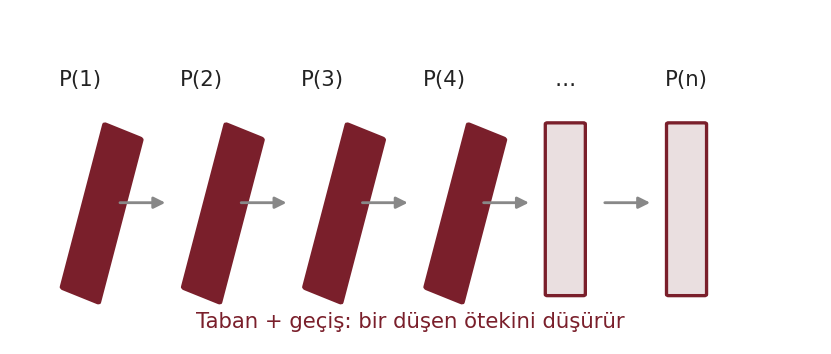
\includegraphics[width=0.85\linewidth]{figs/induction.png}
\caption{Tümevarım: taban durumu ilk taşı düşürür, geçiş adımı zinciri sürdürür.}
\end{figure}

\section{Zayıf Tümevarım Örnekleri}

\begin{tcolorbox}[bookbox,colback=cEx]\textbf{\textsf{\textcolor{cAcc}{Örnek.}}}\quad İddia: 1 + 2 + … + n = n(n+1)/2.\par\medskip{}Taban: n = 1 için sol taraf 1, sağ taraf 1·2/2 = 1. ✓\par\medskip{}Adım: P(k) doğru olsun. O hâlde 1 + … + k + (k+1) = k(k+1)/2 + (k+1) = (k+1)(k+2)/2, yani P(k+1) doğru. Böylece her n için doğrudur. ∎\end{tcolorbox}

\begin{tcolorbox}[bookbox,colback=cEx]\textbf{\textsf{\textcolor{cAcc}{Örnek.}}}\quad İddia: Her n ≥ 1 için 6 | (n³ − n).\par\medskip{}Taban: n = 1 için n³ − n = 0, 6’ya bölünür. ✓\par\medskip{}Adım: (k+1)³ − (k+1) = (k³ − k) + 3k(k+1). Birinci terim tümevarım varsayımıyla 6’ya bölünür; k(k+1) ardışık iki tam sayı olduğundan çifttir, dolayısıyla 3k(k+1) 6’ya bölünür. Toplam 6’ya bölünür. ∎\end{tcolorbox}

\section{Güçlü Tümevarım}\label{sec:guclu}

Güçlü tümevarımda, P(k+1)’i ispatlarken yalnızca P(k) değil, P(1), …, P(k)’nin tümü varsayılır. Bu, taban durumundan k+1’e kadar tüm önceki durumlara dayanmayı gerektiren ispatlarda kullanılır.

\begin{tcolorbox}[bookbox,colback=cEx]\textbf{\textsf{\textcolor{cAcc}{Örnek.}}}\quad İddia: Her n ≥ 2 doğal sayısı asalların çarpımı olarak yazılabilir.\par\medskip{}İspat (güçlü tümevarım): Taban n = 2 asaldır. n = k+1 için: ya k+1 asaldır (bitti), ya da k+1 = a·b, 2 ≤ a, b ≤ k. Tümevarım varsayımıyla a ve b asal çarpımıdır; öyleyse k+1 de asal çarpımıdır. ∎\end{tcolorbox}

\begin{tcolorbox}[bookbox,colback=cDep]\textbf{\textsf{\textcolor{cAcc}{Muhakeme/Felsefe Derinleştirmesi — Matematiksel tümevarım neden tümdengelimseldir?}}}\quad Adı yanıltıcıdır. Bölüm~\ref{chap:muhakeme-turleri}’de tümevarımsal muhakemenin sonucu yalnızca desteklediğini, garanti etmediğini görmüştük. Oysa matematiksel tümevarım, sonlu iki adımdan (taban + geçiş) hareketle sonsuz çoklukta önermenin doğruluğunu \emph{zorunlu} olarak türetir; hiçbir örneği ‘tek tek deneyip genellemez’. Bu yüzden tam anlamıyla tümdengelimsel bir çıkarımdır ve iyi sıralama ilkesine dayanır. Öğrencinin bu terim karışıklığını fark etmesi, muhakeme türleri ile ispat yöntemleri arasındaki köprüyü kurar.\end{tcolorbox}

\section{İleri Örnekler: Farklı Tümevarım Türleri}

Tümevarım yalnızca toplam formüllerinde değil; bölünebilirlik, eşitsizlik ve varlık iddialarında da çalışır. Aşağıdaki örnekler tekniğin kapsamını gösterir.

\begin{tcolorbox}[bookbox,colback=cEx]\textbf{\textsf{\textcolor{cAcc}{Örnek.}}}\quad Geometrik toplam: r ≠ 1 için 1 + r + r² + … + rⁿ = (r\textasciicircum{}(n+1) − 1)/(r − 1).\par\medskip{}Taban n = 0: sol taraf 1, sağ taraf (r − 1)/(r − 1) = 1. ✓  Adım: toplama rᵏ⁺¹ eklenirse (rᵏ⁺¹ − 1)/(r − 1) + rᵏ⁺¹ = (rᵏ⁺¹ − 1 + rᵏ⁺²  − rᵏ⁺¹)/(r − 1) = (rᵏ⁺² − 1)/(r − 1). Böylece formül n = k+1 için de doğrudur. ∎\end{tcolorbox}

\begin{tcolorbox}[bookbox,colback=cEx]\textbf{\textsf{\textcolor{cAcc}{Örnek.}}}\quad Bölünebilirlik: her n ≥ 1 için 3 | (n³ + 2n).\par\medskip{}Taban n = 1: 1 + 2 = 3, 3’e bölünür. ✓  Adım: (k+1)³ + 2(k+1) = (k³ + 2k) + 3(k² + k + 1). Birinci terim tümevarım varsayımıyla 3’e bölünür; ikinci terim açıkça 3’ün katıdır. Toplam 3’e bölünür. ∎\end{tcolorbox}

\begin{tcolorbox}[bookbox,colback=cEx]\textbf{\textsf{\textcolor{cAcc}{Örnek.}}}\quad Eşitsizlik: her n ≥ 4 için n! > 2ⁿ.\par\medskip{}Taban n = 4: 24 > 16. ✓  Adım: (k+1)! = (k+1)·k! > (k+1)·2ᵏ. k ≥ 4 olduğundan k + 1 ≥ 5 > 2, dolayısıyla (k+1)·2ᵏ > 2·2ᵏ = 2ᵏ⁺¹. Böylece (k+1)! > 2ᵏ⁺¹. ∎\end{tcolorbox}

\begin{tcolorbox}[bookbox,colback=cEx]\textbf{\textsf{\textcolor{cAcc}{Örnek.}}}\quad Güçlü tümevarımla varlık: her n ≥ 8 tam sayısı 3a + 5b (a, b ≥ 0 tam sayı) biçiminde yazılabilir.\par\medskip{}Taban: 8 = 3 + 5, 9 = 3·3, 10 = 5·2. Adım: n ≥ 11 için n − 3 ≥ 8’dir; tümevarım varsayımıyla n − 3 = 3a + 5b yazılır, buna bir 3 eklenerek n = 3(a+1) + 5b elde edilir. Üç ardışık taban durumu, adımın ‘üç geri’ gitmesini karşıladığı için gereklidir. ∎\end{tcolorbox}

\begin{tcolorbox}[bookbox,colback=cMis]\textbf{\textsf{\textcolor{cAcc}{Yaygın Kavram Yanılgıları}}}\quad \textbf{“Taban adımını atlayabilirim.” — }Taban olmadan geçiş boşta kalır; ‘tüm sayılar birbirine eşittir’ gibi saçma sonuçlar taban eksikliğinden doğar.\par\medskip{}\textbf{“Tümevarım hipotezi, ispatlamak istediğim şeyi varsaymaktır (döngüsel).” — }Hayır; P(k)’yi varsayıp P(k+1)’i türetmek döngüsel değildir. Sonsuz sayıda ‘eğer-ise’ adımını, iyi sıralama sayesinde tek seferde kurmaktır.\par\medskip{}\textbf{“Tümevarım yalnızca eşitlikler içindir.” — }Bölünebilirlik, eşitsizlik ve varlık iddiaları da tümevarımla kanıtlanır.\par\medskip{}\textbf{“Güçlü ve zayıf tümevarım farklı güçtedir.” — }İkisi mantıksal olarak denktir; ‘güçlü’ biçim yalnızca bazı ispatları kolaylaştırır.\par\medskip{}\textbf{“Adımda n = k+1’i doğrudan hesaplarım.” — }Amaç hesaplamak değil, P(k)’den P(k+1)’i türetmektir; tümevarım hipotezi mutlaka kullanılmalıdır, yoksa ispat tümevarım değildir.\end{tcolorbox}

\section{Uygulama ve Eğitime Yansıma}

Tümevarım, bilgisayar biliminin belkemiğidir: özyinelemeli (recursive) algoritmaların doğruluğu ve döngü değişmezleri (loop invariants) tümevarımla kanıtlanır. Bir öğrenci ‘taban durum + özyineleme adımı’ kalıbını tümevarımla eşleştirdiğinde, hem matematiksel ispatı hem de programlamadaki özyinelemeyi aynı fikrin iki yüzü olarak görür.

Öğretimde en sık görülen iki hata, taban adımının unutulması ve tümevarım hipotezinin hiç kullanılmamasıdır. Öğretmen, öğrenciye ‘hipotezini nerede kullandın?’ sorusunu düzenli sorarak bu boşlukları görünür kılabilir. ‘Tüm atlar aynı renktedir’ gibi klasik sahte ispatlar, hatanın tam olarak hangi adımda saklandığını tartıştırmak için güçlü bir sınıf etkinliğidir.

\section{Yüksek Lisans Derinleştirmesi: İyi Sıralama, Denklik ve Yapısal Tümevarım}

Matematiksel tümevarım ilkesi, iyi sıralama ilkesine denktir: her biri diğerinden türetilebilir. İyi sıralamadan tümevarıma geçiş şöyledir: P(n)’in doğru olmadığı sayılar kümesi S boş değilse, iyi sıralamayla S’nin bir en küçük elemanı m vardır; m > taban olduğundan m − 1 için P doğrudur, ama geçiş adımı P(m)’i verir — çelişki. Demek ki S boştur. Bu denklik, tümevarımın ‘aksiyom’ değil, doğal sayıların düzeninin bir sonucu olduğunu gösterir.

Tümevarım yalnızca sayılarla sınırlı değildir. Yapısal tümevarım (structural induction), özyinelemeli tanımlanan nesneler — ifadeler, ağaçlar, biçimsel diller — üzerinde çalışır: taban durum en basit nesnelerdir, adım ise nesneleri birleştiren kurallardır. Örneğin bir mantık formülünün her alt formülü için bir özelliğin geçerliliği yapısal tümevarımla kanıtlanır. Bu, tümevarımın ‘sıra’ değil, ‘iyi temellendirilmiş (well-founded) bir ilişki’ gerektirdiğini ortaya koyar.

Bu fikrin en genel biçimi sonlu-ötesi (transfinite) tümevarımdır: iyi sıralı herhangi bir küme üzerinde — sıra sayıları (ordinaller) dahil — tümevarım yapılabilir. Böylece ‘taban + geçiş’ şeması, sonlu doğal sayıların çok ötesine, sonsuz ama iyi sıralı yapılara taşınır. Öğretmen adayı için buradaki ders, matematiksel tümevarımın izole bir hüner değil, ‘iyi temellendirilmiş yapılarda tümdengelim’ biçimindeki derin bir ilkenin en tanıdık örneği olduğudur.

\section{Daha Fazla Uygulama: Hanoi, Küpler ve Eşitsizlik}

Tümevarımın kapsamını birkaç klasik örnekle daha genişletelim. Her biri farklı bir problem türünü — sayma, cebirsel özdeşlik, eşitsizlik — temsil eder, ama hepsi aynı taban–geçiş şemasını kullanır.

\begin{tcolorbox}[bookbox,colback=cEx]\textbf{\textsf{\textcolor{cAcc}{Örnek.}}}\quad \textbf{Hanoi Kuleleri. }n diskli Hanoi bulmacası en az 2ⁿ − 1 hamlede çözülür. Taban n = 1: tek disk 2¹ − 1 = 1 hamlede taşınır. Adım: k + 1 diski taşımak için üstteki k diski (varsayımla 2ᵏ − 1 hamle), en alttaki diski (1 hamle) ve k diski tekrar (2ᵏ − 1 hamle) taşırız; toplam 2(2ᵏ − 1) + 1 = 2ᵏ⁺¹ − 1. Bulmacanın özyinelemeli yapısı, tümevarımın doğal habitatıdır. ∎\end{tcolorbox}

\begin{tcolorbox}[bookbox,colback=cEx]\textbf{\textsf{\textcolor{cAcc}{Örnek.}}}\quad \textbf{Küplerin toplamı. }1³ + 2³ + … + n³ = (n(n + 1)/2)². Taban n = 1: 1 = 1². Adım: tümevarım varsayımına (k + 1)³ eklenip düzenlenince ((k + 1)(k + 2)/2)² elde edilir. Şaşırtıcı olan, ilk n küpün toplamının, ilk n sayının toplamının karesi olmasıdır — sayma ve cebir arasında zarif bir köprü. ∎\end{tcolorbox}

\begin{tcolorbox}[bookbox,colback=cEx]\textbf{\textsf{\textcolor{cAcc}{Örnek.}}}\quad \textbf{Bernoulli eşitsizliği. }x ≥ −1 ve n ≥ 0 için (1 + x)ⁿ ≥ 1 + nx. Taban n = 0: 1 ≥ 1. Adım: (1 + x)ᵏ⁺¹ = (1 + x)(1 + x)ᵏ ≥ (1 + x)(1 + kx) = 1 + (k + 1)x + kx² ≥ 1 + (k + 1)x, çünkü kx² ≥ 0. Bu eşitsizlik analizde, limit ve yakınsaklık hesaplarında sürekli kullanılır. ∎\end{tcolorbox}

\section{Özyineleme ve Algoritma Doğruluğu}

Tümevarımın belki en yaygın çağdaş uygulaması bilgisayar bilimindedir. Özyinelemeli (recursive) bir fonksiyon, taban durum ile ‘kendini daha küçük girdide çağırma’ adımından oluşur — tam olarak tümevarımın taban ve geçiş adımlarına karşılık gelir. Bir özyinelemeli algoritmanın doğruluğu, çıktısının doğru olduğu iddiasının tümevarımla kanıtlanmasıyla kurulur; sonlanması ise girdinin her çağrıda ‘iyi temellendirilmiş’ biçimde küçülmesiyle güvence altına alınır.

Aynı fikir döngüler için ‘döngü değişmezi’ (loop invariant) olarak karşımıza çıkar: döngünün her yinelemesinde korunan bir özellik, taban (döngüden önce) ve geçiş (her yineleme) adımlarıyla kanıtlanır; döngü bittiğinde bu değişmez, istenen sonucu verir. Böylece bir öğrenci ‘taban + adım’ kalıbını öğrendiğinde, hem matematiksel bir teoremi kanıtlayabilir hem de bir programın neden doğru çalıştığını gerekçelendirebilir. Tümevarım, bu yönüyle matematik ile hesaplama arasındaki en somut bağlardan biridir ve öğretmen adayına konunun ‘yalnızca formül kanıtlamak’ olmadığını gösterir.

\section{İki Uzun Örnek: Bölünebilirlik ve Karo Döşeme}

Tümevarımın çok yönlülüğünü, biri klasik biri görsel iki örnekle daha pekiştirelim. Bu örnekler, tekniğin cebirden geometriye uzanan kapsamını gösterir.

\begin{tcolorbox}[bookbox,colback=cEx]\textbf{\textsf{\textcolor{cAcc}{Örnek.}}}\quad Bölünebilirlik: her n ≥ 1 için 7 | (8ⁿ − 1).\par\medskip{}Taban n = 1: 8 − 1 = 7, 7’ye bölünür. ✓  Adım: 8ᵏ⁺¹ − 1 = 8·8ᵏ − 1 = 8(8ᵏ − 1) + 7. İlk terim tümevarım varsayımıyla 7’ye bölünür, ikinci terim 7’dir; toplam 7’ye bölünür. ∎  (Aynı sonuç 8 ≡ 1 (mod 7) kongrüansıyla da anında görülür — Bölüm~\ref{chap:kongruanslar}; iki yöntem birbirini aydınlatır.)\end{tcolorbox}

\begin{tcolorbox}[bookbox,colback=cEx]\textbf{\textsf{\textcolor{cAcc}{Örnek.}}}\quad Teleskopik toplam: 1/(1·2) + 1/(2·3) + … + 1/(n(n+1)) = n/(n+1).\par\medskip{}Taban n = 1: 1/(1·2) = 1/2 = 1/2. ✓  Adım: n/(n+1) + 1/((n+1)(n+2)) toplamını paydada birleştirirsek (n(n+2) + 1)/((n+1)(n+2)) = (n+1)²/((n+1)(n+2)) = (n+1)/(n+2). Böylece formül n+1 için de doğrudur. Bu tür toplamlar, her terimin ‘bir öncekini götürdüğü’ teleskopik yapıyı sergiler. ∎\end{tcolorbox}

Şimdi görsel bir örnek: bir 2ⁿ × 2ⁿ satranç tahtasından herhangi bir kare çıkarılırsa, kalan bölge L biçimli üçlü karolarla (her biri üç kareyi kaplayan ‘L-tromino’) tam olarak döşenebilir.

\begin{tcolorbox}[bookbox,colback=cEx]\textbf{\textsf{\textcolor{cAcc}{Örnek.}}}\quad L-tromino döşemesi (güçlü/olağan tümevarım).\par\medskip{}Taban n = 1: 2 × 2 tahtadan bir kare çıkınca geriye tam olarak bir L-tromino biçimi kalır. ✓  Adım: 2ᵏ⁺¹ × 2ᵏ⁺¹ tahtayı dört adet 2ᵏ × 2ᵏ çeyreğe böleriz. Çıkarılan kare bir çeyrektedir; o çeyrek tümevarım varsayımıyla döşenir. Kalan üç çeyreğin merkeze bakan köşelerine bir L-tromino yerleştirerek her birinde ‘çıkarılmış bir kare’ etkisi yaratırız; böylece o üç çeyrek de varsayımla döşenir. ∎  Bu ispat, tümevarımın geometrik bir yapıyı nasıl parçalayıp özyinelemeli biçimde çözdüğünü gösterir.\end{tcolorbox}

Bu üç örnek — cebirsel bölünebilirlik, teleskopik toplam ve geometrik döşeme — tümevarımın tek bir formül türüne bağlı olmadığını gösterir. Ortak olan, problemi ‘bir küçüğüne’ indirgeyip varsayımı kullanmaktır. Öğretmen adayı için buradaki mesaj, tümevarımın ezberlenecek bir kalıp değil, çok farklı bağlamlarda yeniden keşfedilebilecek bir düşünme aracı olduğudur; bu esneklik, öğrencinin yöntemi anlamlı biçimde sahiplenmesinin ön koşuludur.

\begin{tcolorbox}[bookbox,colback=cDef]\textbf{\textsf{\textcolor{cAcc}{Tarihsel Not}}}\quad Matematiksel tümevarımın açık ilk kullanımı çoğu zaman Blaise Pascal’a (1654, Traité du triangle arithmétique) atfedilir; ancak yöntemin izleri Öklid’e, Hintli matematikçilere ve on altıncı yüzyılda Francesco Maurolico’ya kadar uzanır. ‘Tümevarım’ (induction) terimini bu bağlamda İngilizce’ye yerleştiren John Wallis ve Augustus De Morgan oldu. On dokuzuncu yüzyılda Giuseppe Peano ise tümevarımı doğal sayıların tanımlayıcı aksiyomlarından biri hâline getirerek, onu bir ‘hüner’ olmaktan çıkarıp ℕ’nin özünün parçası yaptı.\end{tcolorbox}

\section{Görsel Düşünme ve Hatalı Tümevarımlar}

Tümevarım ilkesini bir kez anlamak kolaydır; onu doğru \emph{kullanmak} ise dikkat ister. Bu kısımda önce zayıf ve güçlü tümevarımın mantıksal yapısını bir şemayla karşılaştırıyor, ardından bir eşitsizlik ailesinin grafiğini inceliyor ve son olarak öğrencilerin en sık düştüğü üç tuzağı çözümlü örneklerle ele alıyoruz.

\begin{figure}[htbp]
\centering
\resizebox{\linewidth}{!}{%
\begin{tikzpicture}[x=1.55cm,y=1cm,p/.style={circle,draw=acc,fill=accl,line width=.8pt,minimum size=9mm,font=\sffamily\small}]
\node[font=\sffamily\small\bfseries,anchor=west] at (-.4,1.15) {Zayıf tümevarım: $P(k)\Rightarrow P(k+1)$};
\foreach \i in {1,...,6}{\node[p] (a\i) at (\i,0) {$P(\i)$};}
\foreach \i [evaluate=\i as \j using int(\i+1)] in {1,...,5}{\draw[arr] (a\i)--(a\j);}
\node[font=\sffamily\small] at (6.8,0) {$\cdots$};
\node[font=\sffamily\small\bfseries,anchor=west] at (-.4,-1.45) {Güçlü tümevarım: $P(1)\wedge\cdots\wedge P(k)\Rightarrow P(k+1)$};
\foreach \i in {1,...,6}{\node[p,draw=grn,fill=grnl] (b\i) at (\i,-2.6) {$P(\i)$};}
\foreach \i in {1,...,5}{\foreach \j in {\i,...,5}{\pgfmathtruncatemacro{\t}{\j+1}
  \ifnum\j=\i \draw[arr,grn] (b\i)--(b\t); \else \draw[arr,grn!70,line width=.5pt] (b\i.south) to[bend right=28] (b\t.south);\fi}}
\node[font=\sffamily\small] at (6.8,-2.6) {$\cdots$};
\node[small lbl,anchor=west,text width=3.2cm] at (7.2,-.2) {Her halka yalnızca bir öncekine dayanır.};
\node[small lbl,anchor=west,text width=3.2cm] at (7.2,-2.8) {Her halka, kendisinden önceki \emph{bütün} halkalara dayanabilir.};
\end{tikzpicture}}%
\caption{Zayıf ve güçlü tümevarımın gerekçelendirme yapısı. Güçlü tümevarım daha fazla varsayım kullanır; ama iki ilke doğal sayılarda birbirine denktir.}
\end{figure}

\begin{ornek}[\textbf{Küplerin toplamı bir karedir.}]
Her $n\ge1$ için
\[
1^3+2^3+\cdots+n^3=\Bigl(\frac{n(n+1)}{2}\Bigr)^2 .
\]
\emph{Taban:} $n=1$ için iki taraf da 1’dir. \emph{Adım:} Eşitlik $n=k$ için doğru olsun. O hâlde
\begin{align*}
\sum_{i=1}^{k+1}i^3&=\frac{k^2(k+1)^2}{4}+(k+1)^3\\
&=\frac{(k+1)^2\bigl(k^2+4k+4\bigr)}{4}=\Bigl(\frac{(k+1)(k+2)}{2}\Bigr)^2 .
\end{align*}
Böylece eşitlik $n=k+1$ için de doğrudur. Sonuç şaşırtıcı bir özdeşlik verir: $1^3+\cdots+n^3=(1+\cdots+n)^2$. Sonucun \emph{keşfi} büyük olasılıkla ilk birkaç değerin ($1,9,36,100$) tam kare olduğunun fark edilmesiyle başlar (tümevarımsal gözlem); \emph{gerekçesi} ise yukarıdaki tümdengelimsel adımdır.
\end{ornek}

\begin{ornek}[\textbf{Bernoulli eşitsizliği: varsayım nerede kullanılıyor?}]
$x\ge-1$ ve $n\ge1$ için $(1+x)^n\ge1+nx$ olduğunu gösterelim. Taban $n=1$ için eşitliktir. $(1+x)^k\ge1+kx$ olsun. Her iki tarafı $1+x$ ile çarpalım:
\[
(1+x)^{k+1}\ \ge\ (1+kx)(1+x)=1+(k+1)x+kx^2\ \ge\ 1+(k+1)x .
\]
İlk eşitsizlikte bir eşitsizliği \emph{negatif olmayan} bir sayıyla çarptık; $x\ge-1$ koşulu tam olarak burada kullanılır. İkinci eşitsizlik $kx^2\ge0$ olgusudur. Koşulu kaldırırsak sonuç bozulabilir: $x=-4$, $n=3$ için $(1+x)^3=-27$ iken $1+3x=-11$ olur ve $-27\ge-11$ yanlıştır. Bir tümevarım ispatında \emph{her varsayımın hangi satırda kullanıldığını} işaretlemek, ispatı anlamanın en kısa yoludur.
\end{ornek}

\begin{figure}[htbp]
\centering
\begin{tikzpicture}
\begin{axis}[width=.82\linewidth,height=5cm,ybar,bar width=6pt,xlabel={$n$},ylabel={değer},xtick={1,...,8},ymin=0,ymax=270,
  axis lines*=left,tick label style={font=\sffamily\scriptsize},label style={font=\sffamily\small},
  legend style={at={(0.03,0.97)},anchor=north west,font=\sffamily\scriptsize,draw=none,fill=none}]
\addplot[fill=acc!70,draw=acc] coordinates {(1,2)(2,4)(3,8)(4,16)(5,32)(6,64)(7,128)(8,256)};
\addplot[fill=warm!60,draw=warm] coordinates {(1,1)(2,4)(3,9)(4,16)(5,25)(6,36)(7,49)(8,64)};
\legend{$2^n$,$n^2$}
\end{axis}
\end{tikzpicture}
\caption{$2^n$ ile $n^2$: $n=3$’te $n^2$ öndedir, $n=2$ ve $n=4$’te eşittirler, $n\ge5$ için $2^n$ kesin olarak büyüktür. ‘Her $n$ için $2^n>n^2$’ yanlış; ‘her $n\ge5$ için’ doğrudur. Taban durumunun seçimi, iddianın kendisinin bir parçasıdır.}
\end{figure}

\subsection{Üç Tipik Hata}

\begin{yanilgi}[Hata 1 — Taban adımını atlamak]
‘$n^2+n+1$ her $n$ için çifttir’ iddiasını düşünelim. Adım kusursuz görünür: $k^2+k+1$ çiftse
\[
(k+1)^2+(k+1)+1=(k^2+k+1)+2(k+1)
\]
de çifttir. Oysa iddia \emph{her} $n$ için yanlıştır: $n^2+n=n(n+1)$ çift olduğundan $n^2+n+1$ daima tektir. Adım ‘boşluğa’ kurulmuş bir köprüdür; hiçbir taş ilk kez düşmemiştir.
\end{yanilgi}

\begin{yanilgi}[Hata 2 — Kanıtlanacak olanı adımda varsaymak]
Bazı öğrenciler adımı şöyle yazar: ‘$P(k+1)$ doğru olsun; o hâlde … öyleyse $P(k)$ doğrudur.’ Bu, gerekirliğin yönünü ters çevirir. Adımda varsayılan $P(k)$’dır; ulaşılması gereken $P(k+1)$’dir. Eşitlik ispatlarında güvenli yol, $P(k+1)$’in sol tarafından başlayıp $P(k)$’yı \emph{kullanarak} sağ tarafa varmaktır.
\end{yanilgi}

\begin{yanilgi}[Hata 3 — Adımın küçük değerlerde çalışmaması]
‘Bütün atlar aynı renktir’ yanıltmacasında (Alıştırma 5’teki ‘herkes aynı yaştadır’ sahte ispatı da aynı yapıdadır) adım, ‘ilk $k$ at’ ile ‘son $k$ at’ gruplarının ortak bir ata sahip olmasına dayanır. Bu, $k\ge2$ için doğrudur ama $k=1$’den $k+1=2$’ye geçişte ortak at yoktur. Adımın \emph{bütün} $k\ge n_0$ değerlerinde geçerli olduğunu denetlemek gerekir; en küçük $k$ değeri çoğu zaman en tehlikeli olanıdır.
\end{yanilgi}

\begin{sinif}[Sınıfta · Tümevarım ispat şablonu]
Aşağıdaki şablonu öğrencilere boş olarak verin ve her ispatta doldurtun. Şablon, ispatın mantıksal iskeletini görünür kılar; özellikle ‘Hipotez nerede kullanıldı?’ satırı, öğrencinin hipotezi gerçekten kullanıp kullanmadığını denetler.
\begin{center}\small
\renewcommand{\arraystretch}{1.25}
\begin{tabularx}{.95\linewidth}{>{\bfseries\raggedright\arraybackslash}p{2.6cm}X}
\toprule
Önerme $P(n)$ & $1+3+\cdots+(2n-1)=n^2$, $n\ge1$\\
Taban & $n=1$: $1=1^2$ \checkmark\\
Hipotez & $1+3+\cdots+(2k-1)=k^2$ olsun.\\
Hedef & $1+3+\cdots+(2k+1)=(k+1)^2$\\
Hipotez nerede kullanıldı? & İlk $k$ terimin toplamı yerine $k^2$ yazıldı.\\
Sonuç & Tümevarım ilkesiyle $P(n)$ her $n\ge1$ için doğrudur.\\
\bottomrule
\end{tabularx}
\end{center}
\end{sinif}

\section*{Alıştırmalar}

\reviewitem{1}{Her n ≥ 1 için 1·2 + 2·3 + … + n(n + 1) = n(n + 1)(n + 2)/3 olduğunu tümevarımla gösterin.}

\reviewitem{2}{Her n ≥ 5 için 2ⁿ > n² olduğunu tümevarımla gösterin (taban durumunu dikkatle seçin).}

\reviewitem{3}{Düzlemdeki n doğru, düzlemi en fazla kaç bölgeye ayırır? Bir formül tahmin edip tümevarımla kanıtlayın.}

\reviewitem{4}{Fibonacci dizisi için Fₙ < 2ⁿ olduğunu güçlü tümevarımla gösterin.}

\reviewitem{5}{“n kişilik her grupta herkes aynı yaştadır” sahte ispatını yazın ve hatanın tam olarak hangi adımda gizlendiğini belirtin.}

\section*{Bölüm Özeti}

\begin{itemize}\setlength{\itemsep}{2pt}\setlength{\parskip}{0pt}
\item Tümevarım taban ve geçiş adımlarından oluşur; güçlü biçimi önceki tüm durumları varsayar.
\item Yöntem, iyi sıralama ilkesine dayanır ve sonsuz önermeyi sonlu adımla türetir.
\item Adına rağmen matematiksel tümevarım tümdengelimsel bir yöntemdir.
\end{itemize}

\section*{Gözden Geçirme Soruları}

\reviewitem{1}{‘Tüm atlar aynı renktir’ sözde ispatındaki hata tümevarımın hangi adımındadır?}

\reviewitem{2}{1 + 3 + 5 + … + (2n−1) = n² eşitliğini tümevarımla ispatlayınız.}

\reviewitem{3}{Neden bazı ispatlarda zayıf tümevarım yetmez de güçlü tümevarım gerekir?}

\section*{Çoktan Seçmeli Sorular}

\mcqq{1}{Tümevarımın hangi adımı ‘P(k) ⇒ P(k+1)’ biçimindedir?}

\mcqo{A}{Taban}

\mcqo{B}{Geçiş (adım)}

\mcqo{C}{Sonuç}

\mcqo{D}{Olumsuzlama}

\mcqa{B}{Geçiş adımı P(k)’den P(k+1)’e götürür.}

\mcqq{2}{Matematiksel tümevarım hangi ilkeye dayanır?}

\mcqo{A}{Seçim aksiyomu}

\mcqo{B}{İyi sıralama ilkesi}

\mcqo{C}{De Morgan}

\mcqo{D}{Modus tollens}

\mcqa{B}{Tümevarım iyi sıralama ilkesine dayanır.}

\mcqq{3}{Muhakeme türü olarak matematiksel tümevarım nedir?}

\mcqo{A}{Tümevarımsal}

\mcqo{B}{Abdüktif}

\mcqo{C}{Tümdengelimsel}

\mcqo{D}{Analojik}

\mcqa{C}{Sonlu adımdan sonsuz sonuç zorunlu türetildiği için tümdengelimseldir.}

\mcqq{4}{Önceki tüm durumları varsayan biçim hangisidir?}

\mcqo{A}{Zayıf tümevarım}

\mcqo{B}{Güçlü tümevarım}

\mcqo{C}{Kontrapozitif}

\mcqo{D}{Doğrudan ispat}

\mcqa{B}{Güçlü tümevarım P(1)…P(k)’nin tümünü varsayar.}

\mcqq{5}{Taban adımı neyi gösterir?}

\mcqo{A}{Genel adımı}

\mcqo{B}{İlk durumun (n = 1) doğruluğunu}

\mcqo{C}{Sonucu}

\mcqo{D}{Olumsuzunu}

\mcqa{B}{Taban, ilk durumun (n=1) doğruluğunu kurar.}

\mcqq{6}{1 + 2 + … + n toplamı neye eşittir?}

\mcqo{A}{n²}

\mcqo{B}{n(n−1)/2}

\mcqo{C}{n(n+1)/2}

\mcqo{D}{2n}

\mcqa{C}{Aritmetik dizi toplamı n(n+1)/2’dir.}

\mcqq{7}{İlk n tek sayının toplamı 1 + 3 + … + (2n−1) neye eşittir?}

\mcqo{A}{n(n+1)/2}

\mcqo{B}{n²}

\mcqo{C}{2n − 1}

\mcqo{D}{n(n+1)}

\mcqa{B}{İlk n tek sayının toplamı n²’dir.}

\mcqq{8}{“Tüm atlar aynı renktir” sözde ispatındaki hata nerededir?}

\mcqo{A}{Taban yanlıştır}

\mcqo{B}{Geçiş adımındaki örtüşme küçük n’de geçersizdir}

\mcqo{C}{Sonuç doğrudur}

\mcqo{D}{İlke yanlıştır}

\mcqa{B}{Örtüşme küçük n’de sağlanmaz; hata geçiş adımındadır.}

\mcqq{9}{6 | (n³ − n) ispatında geçiş adımında 3k(k+1) neden 6’ya bölünür?}

\mcqo{A}{k daima çifttir}

\mcqo{B}{k(k+1) ardışık olduğundan çifttir, 3·çift = 6’nın katı}

\mcqo{C}{3 tek olduğundan}

\mcqo{D}{Bölünmez}

\mcqa{B}{k(k+1) ardışık olduğundan çifttir; 3·çift, 6’ya bölünür.}

\mcqq{10}{“Her n ≥ 2 asalların çarpımıdır” güçlü tümevarımında taban nedir?}

\mcqo{A}{n = 2 asaldır}

\mcqo{B}{n = 1}

\mcqo{C}{n = 0}

\mcqo{D}{Taban gerekmez}

\mcqa{A}{Taban n=2’dir ve 2 asaldır.}

\mcqq{11}{Tümevarım sonsuz çoklukta önermeyi nasıl kanıtlar?}

\mcqo{A}{Hepsini tek tek deneyerek}

\mcqo{B}{Sonlu iki adımla zorunlu türeterek}

\mcqo{C}{Olasılıkla}

\mcqo{D}{Örneklerle}

\mcqa{B}{İki sonlu adım (taban+geçiş) sonsuz önermeyi zorunlu kılar.}

\mcqq{12}{İyi sıralama ilkesi ne der?}

\mcqo{A}{Her küme sıralıdır}

\mcqo{B}{Boştan farklı her ℕ alt kümesinin en küçük elemanı vardır}

\mcqo{C}{ℝ iyi sıralıdır}

\mcqo{D}{Her küme sonludur}

\mcqa{B}{İyi sıralama: ℕ’nin boştan farklı her alt kümesinin en küçüğü vardır.}

\mcqq{13}{Zayıf tümevarımda geçiş adımında ne varsayılır?}

\mcqo{A}{P(1)…P(k) hepsi}

\mcqo{B}{Yalnızca P(k)}

\mcqo{C}{P(k+1)}

\mcqo{D}{Hiçbiri}

\mcqa{B}{Zayıf biçim yalnızca bir önceki durumu (P(k)) varsayar.}

\mcqq{14}{Geçiş adımı ispatlanmazsa ne olur?}

\mcqo{A}{Taban yeterlidir}

\mcqo{B}{İlke değişir}

\mcqo{C}{Sonuç garanti edilmez}

\mcqo{D}{Yine doğrudur}

\mcqa{C}{Geçiş kanıtlanmazsa zincir kırılır, sonuç garanti edilmez.}

\mcqq{15}{2ⁿ > n (n ≥ 1) ifadesi tipik olarak hangi yöntemle kanıtlanır?}

\mcqo{A}{Kontrapozitif}

\mcqo{B}{Tümevarım}

\mcqo{C}{Doğruluk tablosu}

\mcqo{D}{Sayma}

\mcqa{B}{Eşitsizlik n üzerinden tümevarımla kanıtlanır.}

\mcqq{16}{Klasik biçimiyle matematiksel tümevarım hangi sayılarda çalışır?}

\mcqo{A}{Gerçel sayılar}

\mcqo{B}{Doğal sayılar}

\mcqo{C}{Karmaşık sayılar}

\mcqo{D}{İrrasyoneller}

\mcqa{B}{Klasik tümevarım doğal sayılar üzerinde işler.}

\mcqq{17}{Geçiş adımında varsayılan P(k) önermesine ne ad verilir?}

\mcqo{A}{Sonuç}

\mcqo{B}{Tümevarım hipotezi}

\mcqo{C}{Taban}

\mcqo{D}{Aksiyom}

\mcqa{B}{Varsayılan P(k)’ye tümevarım hipotezi denir.}

\mcqq{18}{Bir tümevarım ispatı en az kaç adım içerir?}

\mcqo{A}{Bir}

\mcqo{B}{İki (taban ve geçiş)}

\mcqo{C}{Üç}

\mcqo{D}{Sonsuz}

\mcqa{B}{En az iki adım gerekir: taban ve geçiş.}

\mcqq{19}{Güçlü tümevarım ne zaman gerekir?}

\mcqo{A}{Her zaman}

\mcqo{B}{P(k+1) önceki birden çok duruma bağlıysa}

\mcqo{C}{Hiçbir zaman}

\mcqo{D}{Taban yoksa}

\mcqa{B}{Sonuç önceki birçok duruma bağlıysa güçlü biçim gerekir.}

\mcqq{20}{“Matematiksel tümevarım” adı neden yanıltıcıdır?}

\mcqo{A}{Aslında tümevarımsaldır}

\mcqo{B}{Tümdengelimsel olduğu hâlde ‘tümevarım’ denir}

\mcqo{C}{Abdüktiftir}

\mcqo{D}{Analojiktir}

\mcqa{B}{Yöntem tümdengelimseldir; ‘tümevarım’ adı tarihsel bir yanıltmadır.}


\clearpage

\clearpage

\part{Matematiksel Yapılar Üzerine Muhakeme}
\chapter{Kümeler ve Küme Üzerine Muhakeme}
\label{chap:kumeler}


\par\smallskip{\sffamily\bfseries\color{cAcc}Öğrenme Hedefleri}\nopagebreak

\begin{itemize}\setlength{\itemsep}{2pt}\setlength{\parskip}{0pt}
\item Küme, alt küme ve temel küme işlemlerini biçimsel olarak tanımlayabilme.
\item Küme eşitliğini çift kapsama yöntemiyle ispatlayabilme.
\item Kümeler için De Morgan yasalarını ispatlayabilme.
\end{itemize}

\section*{Bölüme Genel Bakış: Kümeler ve Matematiğin Dili}

Küme kavramı modern matematiğin ortak dilidir; ama bu dil tarihsel olarak geç ve sancılı doğdu. Georg Cantor 1870’lerde sonsuz kümeleri karşılaştırmaya giriştiğinde, ‘bir araya getirilmiş nesneler topluluğu’ fikrini matematiğin merkezine taşıdı. Gottlob Frege bu fikri mantığın temeli yapmayı denedi; ancak Bertrand Russell’ın 1901’de bulduğu paradoks, ‘her özellik bir küme tanımlar’ sezgisinin tutarsız olduğunu gösterdi. Ernst Zermelo’nun 1908’deki aksiyomları ve sonraki Fraenkel katkıları küme kavramını sağlam bir temele oturttu.

Bu bölüm kümeleri sezgisel düzeyde tanıtır, ama biçimsel muhakemeyi — özellikle çift kapsama tekniğini — merkeze alır. Amaç yalnızca küme işlemlerini öğretmek değil; ‘iki kümenin eşit olduğunu nasıl ispatlarız?’ ve ‘en sezgisel görünen ilke neden paradoksa yol açabilir?’ gibi soruları çalışarak öğrenciyi matematiksel titizliğe alıştırmaktır. Küme dili sağlam kurulduğunda, sonraki bütün bölümler (bağıntılar, fonksiyonlar, kardinalite) onun üzerine inşa edilir.

\section{Temel Tanımlar}

\begin{tcolorbox}[bookbox,colback=cDef]\textbf{\textsf{\textcolor{cAcc}{Tanım.}}}\quad Bir A kümesi için x ∈ A, “x, A’nın elemanıdır” demektir. A ⊆ B (A, B’nin alt kümesidir), her x için x ∈ A ⇒ x ∈ B koşuluyla tanımlanır. A = B ancak ve ancak A ⊆ B ve B ⊆ A.\end{tcolorbox}

Boş küme ∅ hiçbir elemanı olmayan kümedir ve her kümenin alt kümesidir. Bir A kümesinin tüm alt kümelerinin kümesine kuvvet kümesi denir ve P(A) ile gösterilir.

\section{Küme İşlemleri}

Birleşim A ∪ B = \{x: x ∈ A ∨ x ∈ B\}; kesişim A ∩ B = \{x: x ∈ A ∧ x ∈ B\}; fark A \textbackslash{} B = \{x: x ∈ A ∧ x ∉ B\}. Evrensel küme U içinde tümleyen Aᶜ = U \textbackslash{} A. Kartezyen çarpım A × B = \{(a, b): a ∈ A, b ∈ B\}.

\begin{figure}[htbp]
\centering
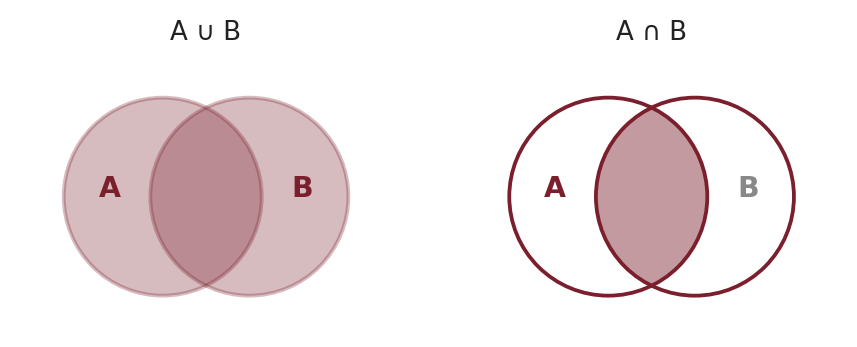
\includegraphics[width=0.85\linewidth]{figs/venn.png}
\caption{Birleşim (A ∪ B) ve kesişim (A ∩ B).}
\end{figure}

\section{Küme Üzerinde İspat: Çift Kapsama}

İki kümenin eşitliğini göstermenin standart yolu her iki kapsamayı ayrı ayrı ispatlamaktır. Bu, küme muhakemesinin temel tekniğidir.

\begin{tcolorbox}[bookbox,colback=cEx]\textbf{\textsf{\textcolor{cAcc}{Örnek.}}}\quad İddia: (A ∪ B)ᶜ = Aᶜ ∩ Bᶜ (De Morgan).\par\medskip{}İspat: x ∈ (A ∪ B)ᶜ ⇔ x ∉ A ∪ B ⇔ ¬(x ∈ A ∨ x ∈ B) ⇔ (x ∉ A) ∧ (x ∉ B) ⇔ x ∈ Aᶜ ∧ x ∈ Bᶜ ⇔ x ∈ Aᶜ ∩ Bᶜ. Her adım bir mantıksal eşdeğerlik olduğundan iki küme aynı elemanlara sahiptir. ∎\end{tcolorbox}

\begin{tcolorbox}[bookbox,colback=cEx]\textbf{\textsf{\textcolor{cAcc}{Örnek.}}}\quad İddia: A ⊆ B ise P(A) ⊆ P(B).\par\medskip{}İspat: X ∈ P(A) olsun, yani X ⊆ A. A ⊆ B olduğundan geçişlilikle X ⊆ B, dolayısıyla X ∈ P(B). Keyfi X için gösterildiğinden P(A) ⊆ P(B). ∎\end{tcolorbox}

\begin{tcolorbox}[bookbox,colback=cDep]\textbf{\textsf{\textcolor{cAcc}{Muhakeme/Felsefe Derinleştirmesi — Naif küme kuramının sınırı: Russell paradoksu}}}\quad “Her özellik bir küme tanımlar” (sınırsız kapsam belirleme) ilkesi çekicidir ama tutarsızdır. R = \{x: x ∉ x\} kümesini düşünün: R ∈ R ise tanımı gereği R ∉ R; R ∉ R ise yine tanımı gereği R ∈ R. Her iki durumda çelişki. Russell’ın 1901’de bulduğu bu paradoks, küme kavramının aksiyomlarla (ZFC) sınırlandırılması gerektiğini gösterdi. Öğrenci için ders şudur: en sezgisel görünen ilke bile denetlenmeden kabul edilemez — bu, dersin ‘aksiyomatik dikkat’ temasının çekirdeğidir.\end{tcolorbox}

\section{İleri Örnekler: Küme Özdeşliklerinin İspatı}

Aşağıdaki örnekler çift kapsama ve eşdeğerlik-zinciri tekniklerini pekiştirir. Her adımda küme işleminin karşılık geldiği mantıksal bağlacı (∩ ↔ ∧, ∪ ↔ ∨, tümleyen ↔ ¬) izlemek, ispatı neredeyse mekanik hâle getirir.

\begin{tcolorbox}[bookbox,colback=cEx]\textbf{\textsf{\textcolor{cAcc}{Örnek.}}}\quad Dağılma yasası: A ∩ (B ∪ C) = (A ∩ B) ∪ (A ∩ C).\par\medskip{}İspat: x ∈ A ∩ (B ∪ C) ⇔ x ∈ A ∧ (x ∈ B ∨ x ∈ C) ⇔ (x ∈ A ∧ x ∈ B) ∨ (x ∈ A ∧ x ∈ C) ⇔ x ∈ (A ∩ B) ∪ (A ∩ C). Ortadaki adım, ‘ve’nin ‘veya’ üzerine dağılmasıdır; küme özdeşliği doğrudan mantıksal dağılmadan gelir. ∎\end{tcolorbox}

\begin{tcolorbox}[bookbox,colback=cEx]\textbf{\textsf{\textcolor{cAcc}{Örnek.}}}\quad Farkın dağılması: A \textbackslash{} (B ∪ C) = (A \textbackslash{} B) ∩ (A \textbackslash{} C).\par\medskip{}İspat: x ∈ A \textbackslash{} (B ∪ C) ⇔ x ∈ A ∧ ¬(x ∈ B ∨ x ∈ C) ⇔ x ∈ A ∧ x ∉ B ∧ x ∉ C ⇔ (x ∈ A ∧ x ∉ B) ∧ (x ∈ A ∧ x ∉ C) ⇔ x ∈ (A \textbackslash{} B) ∩ (A \textbackslash{} C). ∎\end{tcolorbox}

\begin{tcolorbox}[bookbox,colback=cEx]\textbf{\textsf{\textcolor{cAcc}{Örnek.}}}\quad Kesişim ve kuvvet kümesi: P(A ∩ B) = P(A) ∩ P(B).\par\medskip{}İspat: X ∈ P(A ∩ B) ⇔ X ⊆ A ∩ B ⇔ (X ⊆ A) ∧ (X ⊆ B) ⇔ X ∈ P(A) ∧ X ∈ P(B) ⇔ X ∈ P(A) ∩ P(B). Buna karşılık P(A ∪ B) = P(A) ∪ P(B) genelde YANLIŞTIR: A = \{1\}, B = \{2\} için \{1,2\} ∈ P(A ∪ B) iken P(A) ∪ P(B)’de değildir. ∎\end{tcolorbox}

\begin{tcolorbox}[bookbox,colback=cEx]\textbf{\textsf{\textcolor{cAcc}{Örnek.}}}\quad Sonlu sayma (içerme–dışarma): |A ∪ B| = |A| + |B| − |A ∩ B|.\par\medskip{}Gözlem: A ∪ B’yi ayrık parçalara ayırırsak (yalnız A, yalnız B, ortak) her elemanı tam bir kez sayarız; |A| + |B| toplamı ortak elemanları iki kez saydığından bir kez geri çıkarılır. Bu ilke olasılık ve kombinatorikte sürekli kullanılır.\end{tcolorbox}

\begin{tcolorbox}[bookbox,colback=cMis]\textbf{\textsf{\textcolor{cAcc}{Yaygın Kavram Yanılgıları}}}\quad \textbf{“∈ ile ⊆ aynı şeydir.” — }‘∈’ eleman olmayı, ‘⊆’ alt küme olmayı belirtir. 1 ∈ \{1,2\} doğrudur ama 1 ⊆ \{1,2\} anlamsızdır; \{1\} ⊆ \{1,2\} doğrudur.\par\medskip{}\textbf{“∅ ile \{∅\} aynıdır.” — }∅ elemanı olmayan kümedir; \{∅\} ise bir elemanı (boş kümeyi) olan kümedir. Dolayısıyla |\{∅\}| = 1.\par\medskip{}\textbf{“A ⊆ B ise A ∈ B’dir.” — }Alt küme olmak eleman olmayı gerektirmez. \{1\} ⊆ \{1,2\} doğrudur ama \{1\} ∈ \{1,2\} yanlıştır.\par\medskip{}\textbf{“P(A ∪ B) = P(A) ∪ P(B).” — }Genelde yanlıştır; kuvvet kümesi kesişimle uyumludur, birleşimle değil (yukarıdaki örnek).\par\medskip{}\textbf{“Kümenin elemanları sıralı ve tekrarlıdır.” — }Küme sıralamaya ve tekrara duyarsızdır: \{1,2,2,3\} = \{3,1,2\}. Sıra ve tekrar için diziler/çokküme kullanılır.\end{tcolorbox}

\section{Uygulama ve Eğitime Yansıma}

Küme dili, modern matematiğin ortak dilidir: fonksiyon, bağıntı, olasılık, topoloji ve cebir bu dille tanımlanır. Bu yüzden küme kavramını sağlam kurmak, sonraki her bölümün ön koşuludur. Eğitim açısından Venn şemaları, öğrenciyi görsel düzeyden (van Hiele 1) işlemleri çözümlemeye (2. düzey) taşıyan doğal bir köprüdür; ancak öğretmen, şemanın bir ispat değil bir sezgi aracı olduğunu vurgulamalı ve öğrenciyi çift kapsama gibi biçimsel gerekçeye yönlendirmelidir.

Ayrıca küme işlemleri, bilgisayar biliminde (veri tabanı sorguları, arama kümeleri) ve olasılıkta (olayların birleşimi/kesişimi) doğrudan kullanılır. Öğrenciye bu bağlantıları göstermek, soyut küme cebrini somut bir amaca bağlar ve motivasyonu güçlendirir.

\section{Yüksek Lisans Derinleştirmesi: Aksiyomatik Küme Kuramına Giriş}

Russell paradoksu, ‘her özellik bir küme tanımlar’ ilkesinin terk edilmesini zorunlu kıldı. Bunun yerine modern matematik, Zermelo–Fraenkel aksiyomlarını (seçim aksiyomuyla birlikte ZFC) benimser. Bu aksiyomlar hangi kümelerin var olduğunu denetimli biçimde belirler: genişleme (kümeler elemanlarıyla belirlenir), eşleme, birleşim, kuvvet kümesi, ayırma (bir kümenin bir özelliği sağlayan alt kümesi vardır — ama ‘her özellik’ bir küme vermez), sonsuzluk, düzenlilik ve seçim. ‘Ayırma’ aksiyomu, paradoksu tam da sınırsız kapsamı yasaklayarak engeller.

Bu çerçevede ‘tüm kümelerin kümesi’ gibi nesneler küme değil, ‘gerçek sınıf’ (proper class) olarak adlandırılır; bunlar başka kümelere eleman olamaz ve paradoks üretmezler. Küme–sınıf ayrımı, sezgisel ‘topluluk’ kavramının neden dikkatle sınırlandırılması gerektiğinin biçimsel karşılığıdır.

Çarpıcı olan, tüm matematiğin bu kümeler üzerine kodlanabilmesidir. Doğal sayılar bile kümelerle inşa edilir (von Neumann): 0 = ∅, 1 = \{∅\}, 2 = \{∅, \{∅\}\} ve genel olarak n + 1 = n ∪ \{n\}. Böylece her n, kendisinden küçük tüm doğal sayıların kümesidir ve |n| = n olur. Sıralı ikili (a, b) = \{\{a\}, \{a, b\}\} tanımıyla fonksiyonlar da kümeye indirgenir. Bu, kümeler kuramının neden matematiğin ‘temeli’ sayıldığını gösterir: en soyut yapılar bile, denetimli birkaç aksiyomdan doğan kümelerle ifade edilebilir.

\section{Simetrik Fark ve İndeksli İşlemler}

İki kümenin simetrik farkı A △ B = (A \textbackslash{} B) ∪ (B \textbackslash{} A), yani ‘tam olarak birinde bulunan’ elemanlardır. Simetrik fark değişmeli ve birleşmelidir; boş küme onun etkisiz elemanıdır (A △ ∅ = A) ve her küme kendisinin tersidir (A △ A = ∅). Bu özellikler, bir U kümesinin alt kümelerinin simetrik fark altında bir grup oluşturmasını sağlar — küme cebrinin cebirsel yapıya açıldığı ilk noktalardan biri.

\begin{tcolorbox}[bookbox,colback=cEx]\textbf{\textsf{\textcolor{cAcc}{Örnek.}}}\quad \textbf{Simetrik fark. }A = \{1, 2, 3\}, B = \{3, 4, 5\} için A \textbackslash{} B = \{1, 2\}, B \textbackslash{} A = \{4, 5\}, dolayısıyla A △ B = \{1, 2, 4, 5\}. Ortak eleman 3 dışarıda kalır; simetrik fark tam olarak ‘ortak olmayanları’ toplar.\end{tcolorbox}

İşlemler ikiden çok kümeye de genişler. Bir I indeks kümesi ve her i ∈ I için bir Aᵢ kümesi verildiğinde, birleşim ∪\_\{i∈I\} Aᵢ ‘en az bir Aᵢ’de bulunan’, kesişim ∩\_\{i∈I\} Aᵢ ise ‘tüm Aᵢ’lerde bulunan’ elemanlardır. Bu gösterim sonsuz sayıda kümeyle çalışmayı olanaklı kılar ve analiz ile topolojinin temel dilidir.

\begin{tcolorbox}[bookbox,colback=cEx]\textbf{\textsf{\textcolor{cAcc}{Örnek.}}}\quad \textbf{İndeksli kesişim. }Her n ∈ ℕ⁺ için Aₙ = (−1/n, 1/n) açık aralığı alınırsa ∩\_\{n\} Aₙ = \{0\}: her aralıkta bulunan tek nokta sıfırdır. Sonsuz bir kesişim tek bir noktaya ‘sıkışabilir’ — bu, limit fikrinin küme diliyle önizlemesidir.\end{tcolorbox}

Genelleştirilmiş De Morgan yasaları da geçerlidir: (∪\_\{i\} Aᵢ)ᶜ = ∩\_\{i\} Aᵢᶜ ve (∩\_\{i\} Aᵢ)ᶜ = ∪\_\{i\} Aᵢᶜ. Bu eşitlikler, sonlu durumdaki mantıksal çekirdeğin küme diline çevrilmiş hâlidir ve niceleyici olumsuzlama (Bölüm~\ref{chap:niceleyiciler}) ile — ¬(∃x) ⇔ ∀x¬ ve ¬(∀x) ⇔ ∃x¬ — doğrudan koşuttur. Böylece küme cebri ile yüklem mantığı arasındaki bağ görünür hâle gelir.

\section{Sıralı İkili ve Bağıntılara Köprü}

Kümeler yalnızca elemanları toplamakla kalmaz; başka yapıları da kodlar. Sıralı ikili (a, b), Kuratowski’nin tanımıyla \{\{a\}, \{a, b\}\} kümesidir; bu tanım (a, b) = (c, d) ⇔ a = c ∧ b = d özelliğini sağlar. Sıralı ikili sayesinde kartezyen çarpım, dolayısıyla bağıntı ve fonksiyon kavramları (Bölüm~\ref{chap:bagintilar} ve 12) tümüyle küme diline indirgenir.

Bu, kümelerin neden matematiğin ‘temeli’ sayıldığını bir kez daha gösterir: en dinamik görünen kavramlar — bir girdiyi çıktıya götüren fonksiyonlar, nesneler arası ilişkiler — bile statik kümelerle inşa edilebilir. Öğrenci için buradaki ders, soyutlamanın gücüdür: az sayıda ilkel kavram (eleman, küme, ∈) ve denetimli birkaç işlem, matematiğin tümünü taşıyacak kadar zengin bir dil kurar. Bu bölümde öğrenilen çift kapsama tekniği ise, bu dilde ‘kanıt’ yürütmenin en temel aracıdır ve sonraki her bölümde tekrar tekrar kullanılacaktır.

\section{Daha Fazla İspat ve Kanıt Stratejisi Seçimi}

Küme özdeşliklerini kanıtlamanın iki temel yolu vardır: eleman-temelli çift kapsama ve daha önce kanıtlanmış özdeşliklerden cebirsel türetme. Deneyimli bir kanıtlayıcı, probleme göre bu iki strateji arasında geçiş yapar. Aşağıdaki örnekler her iki yolu da gösterir.

\begin{tcolorbox}[bookbox,colback=cEx]\textbf{\textsf{\textcolor{cAcc}{Örnek.}}}\quad Kapsama ile eşitlik: A ⊆ B ⇔ A ∪ B = B.\par\medskip{}İspat (⇒): A ⊆ B varsayalım. A ∪ B ⊆ B göstermek için x ∈ A ∪ B alalım; x ∈ A ise A ⊆ B’den x ∈ B, x ∈ B ise zaten x ∈ B. Ters kapsama B ⊆ A ∪ B her zaman doğrudur. (⇐): A ∪ B = B ise, A ⊆ A ∪ B = B, yani A ⊆ B. Bu eşdeğerlik, ‘alt küme olma’yı bir birleşim eşitliğine çevirdiği için ispatlarda sık kullanılır. ∎\end{tcolorbox}

\begin{tcolorbox}[bookbox,colback=cEx]\textbf{\textsf{\textcolor{cAcc}{Örnek.}}}\quad Karışık işlem: A ∩ (B \textbackslash{} C) = (A ∩ B) \textbackslash{} C.\par\medskip{}İspat: x ∈ A ∩ (B \textbackslash{} C) ⇔ x ∈ A ∧ (x ∈ B ∧ x ∉ C) ⇔ (x ∈ A ∧ x ∈ B) ∧ x ∉ C ⇔ x ∈ (A ∩ B) \textbackslash{} C. Yalnızca ‘ve’ bağlacının birleşme özelliğini kullandık; küme özdeşliği doğrudan mantıksal birleşmeden gelir. ∎\end{tcolorbox}

\begin{tcolorbox}[bookbox,colback=cEx]\textbf{\textsf{\textcolor{cAcc}{Örnek.}}}\quad Cebirsel türetme: (A \textbackslash{} B) ∪ (A ∩ B) = A.\par\medskip{}Daha önce kanıtlanmış dağılma ve tümleyen kurallarıyla: (A \textbackslash{} B) ∪ (A ∩ B) = (A ∩ Bᶜ) ∪ (A ∩ B) = A ∩ (Bᶜ ∪ B) = A ∩ U = A. Burada eleman avlamak yerine bilinen özdeşlikleri zincirledik; bu, daha uzun ifadelerde çoğu zaman daha hızlıdır. ∎\end{tcolorbox}

Strateji seçimi bir muhakeme becerisidir (Bölüm~\ref{chap:muhakeme-turleri}). Kısa ve ‘tanım açma’ gerektiren durumlarda çift kapsama nettir; çok terimli ifadelerde ise bilinen yasaları (dağılma, De Morgan, tümleyen) cebirsel olarak uygulamak daha ekonomiktir. Öğretmen, öğrenciye yalnızca ‘bir’ ispat sunmak yerine iki yolu da göstererek, ispatın tek bir doğru biçimi olmadığını ve yöntem seçiminin kendisinin matematiksel bir karar olduğunu öğretebilir.

Bu bakış, kümeleri sonraki bölümlere de bağlar: aynı ‘tanımı aç, mantıksal eşdeğerlikleri izle, sonucu topla’ ritmi, bağıntı ispatlarında (Bölüm~\ref{chap:bagintilar}), fonksiyon ispatlarında (Bölüm~\ref{chap:fonksiyonlar}) ve kardinalite argümanlarında (Bölüm~\ref{chap:kardinalite}) tekrar tekrar karşımıza çıkacaktır. Küme kanıtlarında ustalaşmak, dolayısıyla dersin geri kalanı için bir tür ‘kanıt gramerinin’ öğrenilmesidir.

\begin{tcolorbox}[bookbox,colback=cDef]\textbf{\textsf{\textcolor{cAcc}{Tarihsel Not}}}\quad Cantor’un sonsuz kümeler kuramı, çağdaşları arasında sert tartışmalara yol açtı. Leopold Kronecker bu kuramı ‘sağlıksız’ bulup Cantor’a şiddetle karşı çıkarken, David Hilbert onu savundu ve ünlü sözünü söyledi: ‘Cantor’un bizim için yarattığı cennetten hiç kimse bizi kovamayacak.’ Bu çekişme, matematiğin temellerine dair yirminci yüzyıl başındaki büyük tartışmanın (mantıkçılık, biçimcilik, sezgicilik) habercisiydi ve küme kuramının neden dikkatli aksiyomlara ihtiyaç duyduğunu gösterdi.\end{tcolorbox}

\section{Venn Diyagramları, Sayma ve Sık Yapılan Hatalar}

Venn diyagramı, küme işlemlerini ‘görmenin’ en eski ve en etkili yoludur. Üç kümeli bir diyagram düzlemi sekiz bölgeye ayırır; her bölge, bir elemanın üç kümenin her birinde bulunup bulunmamasına ilişkin bir ‘evet/hayır’ üçlüsüne karşılık gelir. Bu gözlem, küme cebiri ile önermeler mantığının doğruluk tabloları (Bölüm~\ref{chap:onermeler-mantigi}) arasındaki köprüdür: üç kümeli bir özdeşliği doğrulamak, sekiz satırlık bir doğruluk tablosunu denetlemekle aynı iştir.

\begin{figure}[htbp]
\centering
\begin{tikzpicture}[scale=1.05]
\def\r{1.55}
\coordinate (A) at (-.85,.45); \coordinate (B) at (.85,.45); \coordinate (C) at (0,-1.0);
\draw[line width=.8pt] (-3.3,-3.0) rectangle (3.3,2.55);
\node[font=\sffamily\small,anchor=north west] at (-3.25,2.5) {$U$ (40 öğrenci)};
\fill[acc,opacity=.14] (A) circle (\r); \fill[warm,opacity=.14] (B) circle (\r); \fill[grn,opacity=.14] (C) circle (\r);
\draw[acc,line width=1pt] (A) circle (\r); \draw[warm,line width=1pt] (B) circle (\r); \draw[grn,line width=1pt] (C) circle (\r);
\node[font=\sffamily\bfseries\small,text=acc] at (-2.35,1.75) {$A$};
\node[font=\sffamily\bfseries\small,text=warm] at (2.35,1.75) {$B$};
\node[font=\sffamily\bfseries\small,text=grn] at (1.55,-2.55) {$C$};
\node[font=\sffamily\bfseries] at (-1.55,.85) {9};
\node[font=\sffamily\bfseries] at (1.55,.85) {7};
\node[font=\sffamily\bfseries] at (0,-1.75) {5};
\node[font=\sffamily\bfseries] at (0,1.05) {4};
\node[font=\sffamily\bfseries] at (-.95,-.55) {3};
\node[font=\sffamily\bfseries] at (.95,-.55) {2};
\node[font=\sffamily\bfseries] at (0,.05) {2};
\node[font=\sffamily\bfseries] at (2.7,-2.45) {8};
\end{tikzpicture}
\caption{Üç kümeli Venn diyagramı: sekiz bölge ve aşağıdaki örnekte her bölgedeki öğrenci sayısı. $A$: matematik kulübü, $B$: satranç kulübü, $C$: robotik kulübü.}
\end{figure}

\begin{ornek}[\textbf{İçerme–dışlama ilkesi.}]
40 kişilik bir sınıfta 18 öğrenci matematik ($A$), 15 öğrenci satranç ($B$), 12 öğrenci robotik ($C$) kulübündedir. $|A\cap B|=6$, $|A\cap C|=5$, $|B\cap C|=4$ ve üç kulübe birden katılan 2 öğrenci vardır. En az bir kulübe katılanların sayısı
\begin{align*}
|A\cup B\cup C|&=|A|+|B|+|C|-|A\cap B|-|A\cap C|-|B\cap C|\\
&\quad+|A\cap B\cap C|\\
&=18+15+12-6-5-4+2=32
\end{align*}
olur; hiçbir kulübe katılmayan $40-32=8$ öğrenci vardır. Bölge sayılarını içten dışa doğru bulmak ayrı bir doğrulama sağlar: yalnız $A\cap B$ bölgesi $6-2=4$, yalnız $A$ bölgesi $18-4-3-2=9$ öğrenci içerir. Sekiz bölgenin toplamı $9+7+5+4+3+2+2+8=40$’tır.

\smallskip
\emph{Neden işaretler dönüşümlü?} Üç kümede de bulunan bir öğrenci $|A|+|B|+|C|$ toplamında üç kez sayılır, ikili kesişimlerle üç kez çıkarılır; bu yüzden üçlü kesişimle bir kez geri eklenmelidir. Her elemanın toplamda \emph{tam bir kez} sayıldığını göstermek, formülün ispatıdır.
\end{ornek}

\begin{ornek}[\textbf{Diyagram sezdirir, ispat kanıtlar.}]
Venn diyagramı $A\setminus(B\cup C)=(A\setminus B)\cap(A\setminus C)$ eşitliğini hemen ‘gösterir’: iki taraf da $A$’nın $B$ ve $C$ dışında kalan tek bölgesidir. Ama diyagram özel bir çizimdir; genel ispat eleman takibiyle yapılır:
\begin{align*}
x\in A\setminus(B\cup C)&\iff x\in A\wedge\neg(x\in B\vee x\in C)\\
&\iff (x\in A\wedge x\notin B)\wedge(x\in A\wedge x\notin C).
\end{align*}
İkinci eşdeğerlik De Morgan yasası ve $p\equiv p\wedge p$ eşdeğerliğidir. Diyagram abdüktif bir ipucu, eleman takibi ise tümdengelimsel gerekçedir (Bölüm~\ref{chap:muhakeme-turleri}).
\end{ornek}

\begin{yanilgi}[Yaygın Kavram Yanılgıları]
\textbf{‘$\in$ ile $\subseteq$ aynı şeydir.’} — $1\in\{1,2\}$ doğrudur, $1\subseteq\{1,2\}$ anlamsızdır (1 bir küme değildir); $\{1\}\subseteq\{1,2\}$ doğrudur, $\{1\}\in\{1,2\}$ yanlıştır.

\smallskip
\textbf{‘$\varnothing$ ile $\{\varnothing\}$ aynıdır.’} — Birincisinin hiç elemanı yoktur, ikincisinin bir elemanı vardır. Nitekim $\mathcal P(\varnothing)=\{\varnothing\}$ bir elemanlı, $\mathcal P(\{\varnothing\})=\{\varnothing,\{\varnothing\}\}$ iki elemanlıdır.

\smallskip
\textbf{‘$A\cup B=A\cup C$ ise $B=C$’dir.’} — Sayılarda toplamanın sadeleşme özelliği kümelerde birleşim için geçerli değildir: $A=\{1\}$, $B=\{1\}$, $C=\varnothing$ için $A\cup B=A\cup C$ ama $B\neq C$. (Doğru olan: $A\cup B=A\cup C$ \emph{ve} $A\cap B=A\cap C$ ise $B=C$’dir.)

\smallskip
\textbf{‘Venn diyagramında doğru görünen her şey doğrudur.’} — Dört veya daha çok küme için daireler bütün bölgeleri gösteremez; dört daire en çok 14 bölge oluşturur, oysa dört küme $2^4=16$ bölge gerektirir. Çizimin kapsamı sınırlıdır.
\end{yanilgi}

\begin{sinif}[Sınıfta · Bölge kodları]
Üç kümeli diyagramın sekiz bölgesini öğrencilere $(1,0,1)$ gibi üçlülerle kodlatın ($x\in A$ ise ilk bileşen 1, vb.). Ardından $A\cap(B\cup C)$ ile $(A\cap B)\cup(A\cap C)$ ifadelerinin hangi kodları kapsadığını tablo hâlinde listelesinler. İki listenin aynı çıkması, dağılma özdeşliğinin sekiz satırlık bir ‘doğruluk tablosu’ ispatıdır. Tartışma: ‘Dört küme için kaç satır gerekir? Bu yöntem neden sonsuz sayıda küme için çalışmaz?’
\end{sinif}

\section*{Alıştırmalar}

\reviewitem{1}{A △ (B △ C) = (A △ B) △ C birleşme özelliğini gösterge fonksiyonlarını (mod 2) kullanarak kanıtlayın.}

\reviewitem{2}{|A| = m ve |B| = n ise A’dan B’ye kaç bağıntı, kaç fonksiyon vardır? Yanıtlarınızı (2\textasciicircum{}\{mn\} ve n\textasciicircum{}m) gerekçelendirin.}

\reviewitem{3}{P(A) ∪ P(B) ⊆ P(A ∪ B) olduğunu gösterin ve eşitliğin genelde sağlanmadığına bir karşı örnek verin.}

\reviewitem{4}{∩\_\{n ≥ 1\} [0, 1/n] kümesini bulun ve yanıtınızı gerekçelendirin.}

\reviewitem{5}{Russell paradoksunu, hiç matematik terimi kullanmadan bir arkadaşınıza açıklayacağınız kısa bir benzetme (analoji) yazın.}

\section*{Bölüm Özeti}

\begin{itemize}\setlength{\itemsep}{2pt}\setlength{\parskip}{0pt}
\item Alt küme ve eşitlik, koşullu önerme ve çift kapsamayla tanımlanır.
\item Küme eşitliği ispatının standart tekniği çift kapsamadır; eşdeğerlik zinciriyle de yürütülebilir.
\item Naif kapsam ilkesi Russell paradoksuna yol açar; küme kavramı aksiyomlarla sınırlanır.
\end{itemize}

\section*{Gözden Geçirme Soruları}

\reviewitem{1}{A ∩ B ⊆ A olduğunu eleman alarak ispatlayınız.}

\reviewitem{2}{P(∅) ve P(P(∅)) kümelerini eleman eleman yazınız.}

\reviewitem{3}{A × B ile B × A neden genelde farklıdır? Bir örnekle gösteriniz.}

\section*{Çoktan Seçmeli Sorular}

\mcqq{1}{A = B ispatının standart yöntemi nedir?}

\mcqo{A}{Bir örnek vermek}

\mcqo{B}{Çift kapsama (A⊆B ve B⊆A)}

\mcqo{C}{Doğruluk tablosu}

\mcqo{D}{Tümevarım}

\mcqa{B}{Küme eşitliği çift kapsamayla (A⊆B ve B⊆A) gösterilir.}

\mcqq{2}{Russell paradoksu hangi ilkeyi çürütür?}

\mcqo{A}{Seçim aksiyomu}

\mcqo{B}{Sınırsız kapsam belirleme}

\mcqo{C}{İyi sıralama}

\mcqo{D}{De Morgan}

\mcqa{B}{Sınırsız kapsam ilkesi R=\{x:x∉x\} ile çelişki doğurur.}

\mcqq{3}{n elemanlı bir kümenin kuvvet kümesinin eleman sayısı kaçtır?}

\mcqo{A}{n}

\mcqo{B}{2n}

\mcqo{C}{n²}

\mcqo{D}{2ⁿ}

\mcqa{D}{Her eleman ya vardır ya yoktur: 2ⁿ alt küme.}

\mcqq{4}{(A ∪ B)ᶜ aşağıdakilerden hangisine eşittir?}

\mcqo{A}{Aᶜ ∪ Bᶜ}

\mcqo{B}{Aᶜ ∩ Bᶜ}

\mcqo{C}{A ∩ B}

\mcqo{D}{Aᶜ \textbackslash{} Bᶜ}

\mcqa{B}{De Morgan: birleşimin tümleyeni, tümleyenlerin kesişimidir.}

\mcqq{5}{x ∈ A ∩ B ne anlama gelir?}

\mcqo{A}{x ∈ A veya x ∈ B}

\mcqo{B}{x ∉ A}

\mcqo{C}{x ∈ A ve x ∈ B}

\mcqo{D}{x ∉ B}

\mcqa{C}{Kesişim ‘ve’ demektir: hem A’da hem B’de.}

\mcqq{6}{Boş küme ∅ her kümenin nesidir?}

\mcqo{A}{Elemanı}

\mcqo{B}{Alt kümesi}

\mcqo{C}{Tümleyeni}

\mcqo{D}{Kuvvet kümesi}

\mcqa{B}{∅ her kümenin alt kümesidir.}

\mcqq{7}{A ⊆ B ve B ⊆ A ise ne sonucu çıkar?}

\mcqo{A}{A ⊂ B}

\mcqo{B}{A ∩ B = ∅}

\mcqo{C}{A = B}

\mcqo{D}{A ∪ B = ∅}

\mcqa{C}{Karşılıklı kapsama küme eşitliğini verir.}

\mcqq{8}{A \textbackslash{} B kümesi nedir?}

\mcqo{A}{A ve B’de olanlar}

\mcqo{B}{A’da olup B’de olmayanlar}

\mcqo{C}{A veya B’de olanlar}

\mcqo{D}{Hiçbir eleman}

\mcqa{B}{Fark: A’da olup B’de olmayan elemanlar.}

\mcqq{9}{Kartezyen çarpım A × B’nin elemanları nelerdir?}

\mcqo{A}{a ∪ b}

\mcqo{B}{a ∩ b}

\mcqo{C}{Sıralı ikililer (a, b)}

\mcqo{D}{Alt kümeler}

\mcqa{C}{Kartezyen çarpımın elemanları sıralı ikililerdir.}

\mcqq{10}{De Morgan’a göre (A ∩ B)ᶜ nedir?}

\mcqo{A}{Aᶜ ∪ Bᶜ}

\mcqo{B}{Aᶜ ∩ Bᶜ}

\mcqo{C}{A ∪ B}

\mcqo{D}{∅}

\mcqa{A}{De Morgan: kesişimin tümleyeni, tümleyenlerin birleşimidir.}

\mcqq{11}{A ⊆ B ise kuvvet kümeleri arasındaki ilişki nedir?}

\mcqo{A}{P(A) ⊇ P(B)}

\mcqo{B}{P(A) ⊆ P(B)}

\mcqo{C}{P(A) = P(B)}

\mcqo{D}{İlişki yoktur}

\mcqa{B}{X⊆A⊆B ⇒ X⊆B, yani P(A)⊆P(B).}

\mcqq{12}{P(∅) kümesi nedir?}

\mcqo{A}{∅}

\mcqo{B}{\{∅\}}

\mcqo{C}{\{∅, \{∅\}\}}

\mcqo{D}{Tanımsız}

\mcqa{B}{∅’nin tek alt kümesi kendisidir: P(∅)=\{∅\}.}

\mcqq{13}{“Her x için x ∈ A ⇒ x ∈ B” ifadesi neyi tanımlar?}

\mcqo{A}{A = B}

\mcqo{B}{A ∩ B}

\mcqo{C}{A ⊆ B}

\mcqo{D}{A × B}

\mcqa{C}{Bu koşullu ifade tam olarak A⊆B tanımıdır.}

\mcqq{14}{|A| = 3 ve |B| = 2 ise |A × B| kaçtır?}

\mcqo{A}{5}

\mcqo{B}{8}

\mcqo{C}{6}

\mcqo{D}{9}

\mcqa{C}{|A×B| = |A|·|B| = 3·2 = 6.}

\mcqq{15}{A ∩ A neye eşittir?}

\mcqo{A}{A}

\mcqo{B}{∅}

\mcqo{C}{U}

\mcqo{D}{Aᶜ}

\mcqa{A}{Bir kümenin kendisiyle kesişimi kendisidir.}

\mcqq{16}{A ∪ ∅ neye eşittir?}

\mcqo{A}{∅}

\mcqo{B}{A}

\mcqo{C}{U}

\mcqo{D}{Aᶜ}

\mcqa{B}{Boş kümeyle birleşim kümeyi değiştirmez.}

\mcqq{17}{A ∩ ∅ neye eşittir?}

\mcqo{A}{∅}

\mcqo{B}{A}

\mcqo{C}{U}

\mcqo{D}{Aᶜ}

\mcqa{A}{Boş kümeyle kesişim boştur.}

\mcqq{18}{Naif küme kuramının temel sorunu nedir?}

\mcqo{A}{Her zaman tutarlıdır}

\mcqo{B}{Tutarsızlığa (paradoksa) açıktır}

\mcqo{C}{Sonlu kümelerle sınırlıdır}

\mcqo{D}{Boş kümesi yoktur}

\mcqa{B}{Naif kuram sınırsız kapsamla paradoksa açıktır.}

\mcqq{19}{\{1, 2\} ⊆ \{1, 2, 3\} ifadesi nedir?}

\mcqo{A}{Doğru}

\mcqo{B}{Yanlış}

\mcqo{C}{Tanımsız}

\mcqo{D}{Anlamsız}

\mcqa{A}{\{1,2\}’nin her elemanı \{1,2,3\}’tedir: doğru.}

\mcqq{20}{Her küme için A ⊆ A ifadesi nasıldır?}

\mcqo{A}{Doğru (her küme kendisinin alt kümesidir)}

\mcqo{B}{Yalnızca boş kümede doğru}

\mcqo{C}{Yanlış}

\mcqo{D}{Yalnızca sonlu kümelerde doğru}

\mcqa{A}{Her küme kendisinin alt kümesidir.}


\clearpage

\clearpage
\chapter{Bağıntılar ve Denklik}
\label{chap:bagintilar}


\par\smallskip{\sffamily\bfseries\color{cAcc}Öğrenme Hedefleri}\nopagebreak

\begin{itemize}\setlength{\itemsep}{2pt}\setlength{\parskip}{0pt}
\item İkili bağıntıyı ve temel özelliklerini (yansıma, simetri, geçişlilik) tanımlayabilme.
\item Denklik bağıntısı ile bölümleme arasındaki karşılıklılığı ispatlayabilme.
\end{itemize}

\section*{Bölüme Genel Bakış: İlişkiyi Matematikleştirmek}

‘Daha büyük’, ‘böler’, ‘denktir’, ‘bağlıdır’ — matematiğin ve gündelik dilin büyük bölümü ilişkiler üzerine kuruludur. Bir bağıntı (relation), bu sezgisel ‘ilişki’ fikrini kümeler diliyle kesinleştirir: A × A’nın bir alt kümesi. Charles Sanders Peirce ve Ernst Schröder on dokuzuncu yüzyılda bağıntıların cebirini geliştirdiler; Bourbaki geleneği ise bağıntıyı, fonksiyon dahil pek çok kavramın ortak zemini olarak matematiğin temeline yerleştirdi.

Bu bölüm iki bağıntı ailesine odaklanır: nesneleri ‘aynı sayan’ denklik bağıntıları ve nesneleri ‘sıralayan’ sıralama bağıntıları. İlki soyutlamanın (kesirler, mod sınıfları), ikincisi önceliklendirme ve yapının temelidir. Her ikisi de sonraki bölümlerde — kongrüanslar bir denklik, kardinalite karşılaştırması bir sıralama olarak — yeniden karşımıza çıkar. Böylece bağıntı kavramı, dersin teknik omurgasını birbirine bağlayan zemindir.

\section{Bağıntı ve Özellikleri}

\begin{tcolorbox}[bookbox,colback=cDef]\textbf{\textsf{\textcolor{cAcc}{Tanım.}}}\quad A üzerinde bir (ikili) bağıntı, R ⊆ A × A alt kümesidir; (a, b) ∈ R yerine a R b yazılır. R; yansımalı (her a için a R a), simetrik (a R b ⇒ b R a), ters simetrik (a R b ∧ b R a ⇒ a = b) veya geçişli (a R b ∧ b R c ⇒ a R c) olabilir.\end{tcolorbox}

\section{Denklik Bağıntısı}

Yansımalı, simetrik ve geçişli bir bağıntıya denklik bağıntısı denir. a elemanının denklik sınıfı [a] = \{x ∈ A: x R a\} biçiminde tanımlanır.

\begin{tcolorbox}[bookbox,colback=cDef]\textbf{\textsf{\textcolor{cAcc}{Teorem.}}}\quad Bir A kümesi üzerindeki denklik bağıntısının denklik sınıfları A’yı bir bölümlemeye (boştan farklı, ikişer ayrık, birleşimi A olan alt kümeler) ayırır; tersine, her bölümleme bir denklik bağıntısı tanımlar.\end{tcolorbox}

\begin{tcolorbox}[bookbox,colback=cEx]\textbf{\textsf{\textcolor{cAcc}{Örnek.}}}\quad İspat fikri (sınıflar örtüşmez): [a] ∩ [b] ≠ ∅ olsun; ortak bir c için c R a ve c R b. Simetri ve geçişlilikle a R b, buradan [a] = [b] gösterilir. Ayrıca her a ∈ [a] olduğundan sınıfların birleşimi A’dır. ∎\end{tcolorbox}

\begin{tcolorbox}[bookbox,colback=cDep]\textbf{\textsf{\textcolor{cAcc}{Muhakeme/Felsefe Derinleştirmesi — Sınıflandırma ve soyutlama bir muhakeme biçimi olarak}}}\quad Denklik bağıntısı, matematiğin en güçlü soyutlama araçlarından biridir: ‘aynı sayılacak’ nesneleri tek bir sınıfta toplar ve o sınıfı yeni bir nesne gibi ele almamızı sağlar (kesirler, mod-n sınıfları, yönler…). Bu, öğrencinin gündelik ‘gruplama’ sezgisinden biçimsel soyutlamaya geçişidir ve bir sonraki bölümde kongrüanslarda doğrudan iş görür.\end{tcolorbox}

\section{İleri Örnekler: Denklik, Bölüm Kümesi ve Sıralama}

Bağıntı özelliklerini tanımaktan, onlarla yapı kurmaya geçelim. Aşağıdaki örnekler denklik sınıflarının nasıl yeni nesneler ürettiğini ve sıralama bağıntılarının denklikten nasıl ayrıldığını gösterir.

\begin{tcolorbox}[bookbox,colback=cEx]\textbf{\textsf{\textcolor{cAcc}{Örnek.}}}\quad \textbf{Bölüm kümesi. }ℤ üzerinde a \textasciitilde{} b ⇔ 3 | (a − b) bağıntısı bir denkliktir. Üç denklik sınıfı vardır: [0] = \{…, −3, 0, 3, …\}, [1] = \{…, −2, 1, 4, …\}, [2] = \{…, −1, 2, 5, …\}. Bu sınıfların kümesi ℤ/\textasciitilde{} = \{[0], [1], [2]\} tam olarak ℤ₃’tür. Böylece bir denklik bağıntısı, sonsuz ℤ’den sonlu ve işlem yapılabilir yeni bir nesne üretir.\end{tcolorbox}

\begin{tcolorbox}[bookbox,colback=cEx]\textbf{\textsf{\textcolor{cAcc}{Örnek.}}}\quad \textbf{Kısmi sıralama. }ℕ⁺ üzerinde ‘a, b’yi böler’ (a | b) bağıntısı yansımalı (a | a), ters simetrik (a | b ∧ b | a ⇒ a = b) ve geçişlidir; yani bir kısmi sıralamadır. Ancak tam sıralama değildir: 2 ve 3 birbirini bölmediğinden karşılaştırılamazlar. Bu bağıntının Hasse diyagramında 1 en alttadır, asallar onun hemen üstünde yer alır ve her sayı, bölenlerinin üstüne çizilir.\end{tcolorbox}

\begin{tcolorbox}[bookbox,colback=cEx]\textbf{\textsf{\textcolor{cAcc}{Örnek.}}}\quad \textbf{Kapsama sıralaması. }Bir U kümesinin alt kümeleri üzerinde ‘⊆’ bir kısmi sıralamadır (yansıma, ters simetri, geçişlilik). ∅ en küçük, U en büyük elemandır; ancak iki ayrık küme karşılaştırılamaz olduğundan sıralama tam değildir.\end{tcolorbox}

\begin{tcolorbox}[bookbox,colback=cEx]\textbf{\textsf{\textcolor{cAcc}{Örnek.}}}\quad \textbf{Denklik olmayan bağıntı. }‘x, y ile arkadaştır’ bağıntısı simetriktir ama genelde geçişli değildir (arkadaşımın arkadaşı benim arkadaşım olmayabilir); dolayısıyla bir denklik bağıntısı değildir. Bu, üç özelliğin birbirinden bağımsız olduğunu hatırlatır.\end{tcolorbox}

\begin{tcolorbox}[bookbox,colback=cMis]\textbf{\textsf{\textcolor{cAcc}{Yaygın Kavram Yanılgıları}}}\quad \textbf{“Simetri ve geçişlilik, yansımayı da verir.” — }Yanlış. Bir eleman hiçbir şeyle ilişkili değilse (ör. boş bağıntı), simetri ve geçişlilik sağlansa bile yansıma sağlanmaz.\par\medskip{}\textbf{“Denklik sınıfları örtüşebilir.” — }İki sınıf ya tümüyle özdeştir ya da hiç kesişmez; kısmi örtüşme olamaz.\par\medskip{}\textbf{“Her sıralama tamdır (her iki eleman karşılaştırılabilir).” — }Kısmi sıralamada bazı elemanlar karşılaştırılamaz (2 ve 3, bölme sıralamasında).\par\medskip{}\textbf{“a R b ise her zaman b R a’dır.” — }Bu yalnızca simetrik bağıntılar için doğrudur; sıralamalar simetrik değildir.\par\medskip{}\textbf{“En büyük eleman ile maksimal eleman aynıdır.” — }En büyük eleman herkesten büyüktür; maksimal eleman yalnızca ‘üstünde başka eleman olmayan’dır. Kısmi sıralamada maksimal eleman birden çok olabilir, en büyük eleman ise en fazla bir tanedir.\end{tcolorbox}

\begin{figure}[htbp]
\centering
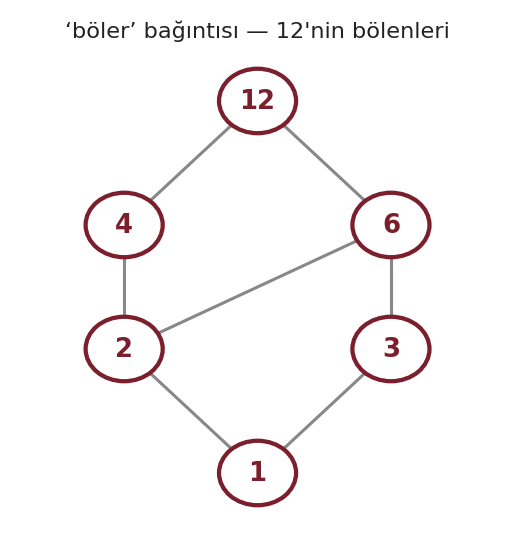
\includegraphics[width=0.56\linewidth]{figs/hasse.png}
\caption{12’nin bölenleri üzerinde ‘böler’ bağıntısının Hasse diyagramı.}
\end{figure}

\section{Uygulama ve Eğitime Yansıma}

Denklik bağıntısı, matematiğin ‘aynı kabul etme’ mekanizmasıdır ve her düzeyde iş görür: kesirler aslında ℤ × ℤ* üzerinde (a, b) \textasciitilde{} (c, d) ⇔ ad = bc denkliğinin sınıflarıdır (1/2 = 2/4 tam da bu yüzden); saat aritmetiği, yönler, geometrik benzerlik hep denklik sınıflarıdır. Öğrenciye ‘eşit olmadıkları hâlde aynı sayılan’ nesneleri fark ettirmek, soyutlamanın ilk ve en önemli adımıdır.

Sıralama bağıntıları ise önceliklendirme, çizelgeleme ve veri sıralama gibi uygulamaların temelidir. Öğretmen, ‘karşılaştırılamaz’ ögelerin bulunabileceği kısmi sıralamaları (ör. görevler arası bağımlılık) somut örneklerle göstererek, öğrencinin ‘her şey bir doğru üzerinde sıralanır’ önyargısını kırabilir.

\section{Yüksek Lisans Derinleştirmesi: Bölüm Kümesi, İyi Tanımlılık ve Sıralama Yapıları}

Bir denklik bağıntısı \textasciitilde{} verildiğinde, A/\textasciitilde{} bölüm kümesi ve π: A → A/\textasciitilde{}, π(a) = [a] kanonik izdüşümü ortaya çıkar. Matematiğin büyük bölümü bu inşa üzerine kuruludur: tam sayılardan rasyonellere, gruplardan bölüm gruplarına, topolojik uzaylardan bölüm uzaylarına. Bu geçişlerde kritik kavram ‘iyi tanımlılık’tır: A/\textasciitilde{} üzerinde bir işlem tanımlarken, sınıf temsilcisinden bağımsız olduğunu göstermek gerekir. Örneğin ℤₙ’de [a] + [b] = [a + b] tanımı ancak kongrüansın toplama ile uyumu (Bölüm~\ref{chap:kongruanslar}) sayesinde iyi tanımlıdır.

Sıralama yapıları da kendi zengin kavramlarını getirir. Bir kısmi sıralamada zincir (ikişer karşılaştırılabilir elemanlar) ve antizincir (ikişer karşılaştırılamaz elemanlar) ayrımı, en büyük/en küçük ile maksimal/minimal ayrımı ve üst/alt sınır kavramları, ileri matematikte (kafes kuramı, Zorn önsavı) merkezî rol oynar. İki sıralı kümenin ‘aynı biçimde sıralandığını’ söylemek için sıralama-koruyan bir eşleme (sıralama izomorfizmi) aranır; bu, Bölüm~\ref{chap:fonksiyonlar}’teki fonksiyon ve Bölüm~\ref{chap:kardinalite}’teki kardinalite fikirlerinin sıralama diline taşınmış hâlidir.

Böylece bağıntılar, dersin geri kalanını birbirine bağlayan zemindir: fonksiyon özel bir bağıntıdır (Bölüm~\ref{chap:fonksiyonlar}), kongrüans bir denkliktir (Bölüm~\ref{chap:kongruanslar}) ve kardinalite karşılaştırması bir tür sıralamadır (Bölüm~\ref{chap:kardinalite}). Bağıntı kavramını sağlam kurmak, bu üç bölümü ortak bir çatı altında görmeyi sağlar.

\section{Bağıntı İşlemleri: Bileşke, Ters ve Kapanış}

Bağıntılar da fonksiyonlar gibi birleştirilebilir ve dönüştürülebilir. Bir R ⊆ A × B ile S ⊆ B × C için bileşke S ∘ R = \{(a, c): ∃b, (a, b) ∈ R ∧ (b, c) ∈ S\} biçiminde tanımlanır. Ters bağıntı ise R⁻¹ = \{(b, a): (a, b) ∈ R\}. Bu işlemler, ilişkileri zincirlemeyi ve yönünü tersine çevirmeyi olanaklı kılar.

\begin{tcolorbox}[bookbox,colback=cEx]\textbf{\textsf{\textcolor{cAcc}{Örnek.}}}\quad \textbf{Bileşke. }R = ‘ebeveynidir’ ve S = ‘ebeveynidir’ ise S ∘ R = ‘büyükebeveynidir’. Bağıntı bileşkesi, ‘iki adımlık ilişkiyi’ tek bir bağıntı olarak ifade eder.\end{tcolorbox}

Bir bağıntı istenen bir özelliği sağlamıyorsa, onu sağlayan ‘en küçük’ genişlemesi aranabilir; buna kapanış (closure) denir. Yansımalı kapanış eksik olan (a, a) çiftlerini ekler; geçişli kapanış ise dolaylı olarak bağlı tüm çiftleri ekler. Örneğin bir yol ağında ‘doğrudan bağlantı’ bağıntısının geçişli kapanışı ‘bir yolla ulaşılabilir’ bağıntısını verir — bu, bilgisayar biliminde ulaşılabilirlik hesaplarının tam karşılığıdır.

\begin{tcolorbox}[bookbox,colback=cEx]\textbf{\textsf{\textcolor{cAcc}{Örnek.}}}\quad \textbf{Geçişli kapanış. }A = \{1, 2, 3\} üzerinde R = \{(1,2), (2,3)\} bağıntısı geçişli değildir. Geçişli kapanışı R⁺ = \{(1,2), (2,3), (1,3)\}; dolaylı bağ (1,3) eklenir. Bir denklik bağıntısı üretmek istersek ayrıca yansıma ve simetri kapanışlarını da almamız gerekir.\end{tcolorbox}

\section{Sıralama Türleri: Kısmi, Tam ve İyi Sıralama}

Sıralama bağıntıları kendi içinde katmanlıdır. Bir kısmi sıralamada (yansıma, ters simetri, geçişlilik) bazı elemanlar karşılaştırılamaz olabilir. Eğer her iki eleman karşılaştırılabiliyorsa sıralama tamdır (doğrusaldır): ℝ üzerindeki ‘≤’ böyledir. Bir adım ötede, boştan farklı her alt kümenin bir en küçük elemanı varsa sıralama iyi sıralamadır.

Bu ayrımlar önemlidir: ℕ, ‘≤’ ile iyi sıralıdır (Bölüm~\ref{chap:tumevarim}’daki tümevarımın dayanağı budur), ama ℤ ve ℝ tam sıralı oldukları hâlde iyi sıralı değildir — negatif tam sayılar kümesinin en küçüğü yoktur, (0, 1) açık aralığının da. İyi sıralama, seçim aksiyomuyla birlikte matematiğin derin sonuçlarına (her kümenin iyi sıralanabileceği, Zorn önsavı) bağlanır. Böylece Bölüm~\ref{chap:bagintilar}, sıradan ‘büyüklük karşılaştırması’ndan başlayıp modern matematiğin temel yapı taşlarına uzanan bir yelpazeyi kapsar; bu yapılar Bölüm~\ref{chap:fonksiyonlar}’teki fonksiyon ve Bölüm~\ref{chap:kardinalite}’teki kardinalite dilinde yeniden iş görür.

\section{Denklik Sınıflarıyla İnşa: Sayı Sistemleri}

Denklik bağıntısının matematikteki en güçlü uygulamalarından biri, yeni sayı sistemlerini eski olanlardan ‘kurmasıdır’. Bu inşalar, kesirlerin ve negatif sayıların aslında birer denklik sınıfı olduğunu ortaya koyar ve öğrencinin ‘sayı’ kavramına bakışını kökten değiştirir.

Tam sayıları doğal sayılardan kurmak için ℕ × ℕ üzerinde (a, b) \textasciitilde{} (c, d) ⇔ a + d = b + c bağıntısını tanımlarız. Buradaki sezgi, (a, b) çiftinin ‘a − b farkını’ temsil etmesidir; a + d = b + c koşulu, kesme (çıkarma) yapmadan ‘iki farkın eşitliğini’ yalnızca toplama diliyle ifade eder. Bu bağıntı bir denkliktir ve sınıfları tam sayıları verir: örneğin [(3, 5)] ile [(0, 2)] aynı sınıftır ve her ikisi de −2 tam sayısına karşılık gelir. Toplama ve çarpma, temsilcilerden bağımsız (iyi tanımlı) biçimde bu sınıflar üzerine taşınır.

Aynı fikir rasyonel sayıları verir. ℤ × ℤ* (paydası sıfırdan farklı çiftler) üzerinde (a, b) \textasciitilde{} (c, d) ⇔ ad = bc bağıntısı bir denkliktir ve sınıfları kesirlerdir. Burada 1/2 = 2/4 eşitliğinin gerçek anlamı ortaya çıkar: (1, 2) ile (2, 4) aynı denklik sınıfının iki temsilcisidir, çünkü 1·4 = 2·2. Yani ‘kesir sadeleştirme’ dediğimiz şey, aslında aynı denklik sınıfının farklı temsilcileri arasında geçiş yapmaktır.

\begin{tcolorbox}[bookbox,colback=cEx]\textbf{\textsf{\textcolor{cAcc}{Örnek.}}}\quad \textbf{İyi tanımlılık neden gerekir? }ℚ’de toplama [(a, b)] + [(c, d)] = [(ad + bc, bd)] biçiminde tanımlanır. Bu tanımın anlamlı olması için, temsilci değiştirdiğimizde sonucun değişmemesi gerekir. Örneğin 1/2 yerine 2/4 kullanırsak toplam yine aynı sınıfı vermelidir; bunu doğrulamak, denklik koşulunun (ad = bc) işlemle uyumunu göstermektir. İşte bu ‘iyi tanımlılık’ kontrolü, bölüm kümeleriyle çalışmanın değişmez bir parçasıdır.\end{tcolorbox}

Bu inşalar pedagojik olarak da aydınlatıcıdır. Öğrenciler çoğu zaman negatif sayıları ve kesirleri ‘gökten inmiş’ nesneler olarak öğrenir; oysa denklik sınıfı bakışı, bunların doğal sayılardan sistemli biçimde üretilebildiğini gösterir. Aynı desen ileride devam eder: gerçel sayılar rasyonellerin belirli dizilerinin denklik sınıflarıyla (Cauchy dizileri) kurulur. Böylece ‘denklik sınıfıyla inşa’, tek bir konu değil, matematiğin sayı sistemlerini büyütme yöntemidir.

Sonuç olarak Bölüm~\ref{chap:bagintilar}’in denklik bağıntısı, Bölüm~\ref{chap:kongruanslar}’nin kongrüans sınıflarıyla (ℤₙ) ve dersin sayı kavramına dair tüm tartışmasıyla derinden bağlantılıdır. Öğretmen adayı, ‘aynı kabul etme’nin biçimsel karşılığı olan denklik sınıfını kavradığında, hem soyut cebirin kapısını aralamış hem de okul matematiğindeki kesir ve tam sayı öğretimine çok daha derin bir zeminden bakabilir hâle gelmiş olur.

\begin{tcolorbox}[bookbox,colback=cDef]\textbf{\textsf{\textcolor{cAcc}{Tarihsel Not}}}\quad Bağıntıların matematiksel kuramı, on dokuzuncu yüzyılda Augustus De Morgan, Charles Sanders Peirce ve Ernst Schröder’in ‘bağıntı cebri’ çalışmalarıyla olgunlaştı. Aynı dönemde Richard Dedekind, gerçel sayıları rasyonellerin bir sıralama-bölünmesi (‘Dedekind kesitleri’) olarak tanımladı — sıralama bağıntısının, sayı sistemlerini kurmakta ne denli temel olduğunun çarpıcı bir örneği. Bugün bağıntı kavramı, veri tabanlarından graf kuramına kadar hesaplamalı matematiğin de ortak dilidir.\end{tcolorbox}

\section{Bağıntıları Görmek: Yönlü Graf ve Matris}

Sonlu bir küme üzerindeki bir bağıntı iki farklı biçimde ‘çizilebilir’: \emph{yönlü graf} olarak (her eleman bir nokta, her $(a,b)\in R$ çifti $a$’dan $b$’ye bir ok) ve \emph{bağıntı matrisi} olarak ($a$ satırı ile $b$ sütununun kesiştiği yere $(a,b)\in R$ ise 1, değilse 0). Bağıntının özellikleri bu iki temsilde gözle okunabilir; bu da soyut tanımları somut denetimlere dönüştürür.

\begin{figure}[htbp]
\centering
\begin{tikzpicture}[v/.style={circle,draw=acc,fill=accl,line width=.8pt,minimum size=7mm,font=\sffamily\small},>={Stealth[length=5pt]}]
\node[v] (1) at (0,1.6) {1}; \node[v] (2) at (1.8,1.6) {2};
\node[v] (3) at (0,0) {3}; \node[v] (4) at (1.8,0) {4};
\path[->,line width=.8pt,draw=bar] (1) edge[loop left,min distance=5mm] (1) (3) edge[loop left,min distance=5mm] (3) (2) edge[loop right,min distance=5mm] (2) (4) edge[loop right,min distance=5mm] (4);
\draw[->,line width=.8pt,bar] (1) to[bend left=18] (2); \draw[->,line width=.8pt,bar] (2) to[bend left=18] (1);
\draw[->,line width=.8pt,bar] (3) to[bend left=18] (4); \draw[->,line width=.8pt,bar] (4) to[bend left=18] (3);
\begin{scope}[on background layer]
\fill[grnl,rounded corners=8pt] (-.75,1.05) rectangle (2.55,2.2);
\fill[warml,rounded corners=8pt] (-.75,-.6) rectangle (2.55,.55);
\end{scope}
\node[anchor=west] at (3.6,.8) {$M_R=\begin{pmatrix}1&1&0&0\\1&1&0&0\\0&0&1&1\\0&0&1&1\end{pmatrix}$};
\node[small lbl,anchor=north] at (.9,-1.0) {yönlü graf};
\node[small lbl,anchor=north] at (5.1,-1.0) {bağıntı matrisi};
\end{tikzpicture}
\caption{$\{1,2,3,4\}$ üzerinde $R=\{(1,1),(2,2),(3,3),(4,4),$\allowbreak$(1,2),(2,1),(3,4),(4,3)\}$ bağıntısı. Her köşede döngü (yansıma), her ok çift yönlü (simetri); iki renkli bölge iki denklik sınıfıdır: $\{1,2\}$ ve $\{3,4\}$. Matriste sınıflar köşegen üzerindeki bloklar olarak görünür.}
\end{figure}

\begin{table}[htbp]
\centering\small
\renewcommand{\arraystretch}{1.3}
\begin{tabularx}{\linewidth}{>{\raggedright\arraybackslash}p{2.1cm}>{\raggedright\arraybackslash}X>{\raggedright\arraybackslash}X}
\toprule
\textbf{Özellik} & \textbf{Yönlü grafta} & \textbf{Matriste}\\
\midrule
Yansıma & Her noktada bir döngü vardır. & Köşegendeki bütün girdiler 1’dir.\\
Simetri & Her okun ters yönlüsü de vardır. & $M=M^{\mathsf T}$ (köşegene göre simetrik).\\
Ters simetri & Farklı iki nokta arasında en fazla bir yönde ok vardır. & $i\neq j$ için $m_{ij}$ ve $m_{ji}$ ikisi birden 1 olamaz.\\
Geçişlilik & $a\to b\to c$ yolu varsa $a\to c$ oku da vardır. & Boole çarpımı $M\odot M$’de 1 olan her yer $M$’de de 1’dir.\\
\bottomrule
\end{tabularx}
\caption{Bağıntı özelliklerinin iki temsilde okunması.}
\end{table}

\begin{ornek}[\textbf{Geçişli kapanış.}]
$\{1,2,3,4\}$ üzerinde $S=\{(1,2),(2,3),(3,4)\}$ bağıntısı geçişli değildir: $1\to2\to3$ yolu vardır ama $(1,3)\notin S$. $S$’yi kapsayan en küçük geçişli bağıntıyı (geçişli kapanış $S^+$) bulmak için, iki adımlı yollarla ulaşılabilen çiftleri ekleriz: $(1,3)$, $(2,4)$; ardından üç adımlı yolla $(1,4)$. Böylece
\[
S^+=\{(1,2),(2,3),(3,4),(1,3),(2,4),(1,4)\}
\]
olur. Grafta bu, ‘bir yol varsa doğrudan ok çiz’ kuralıdır. $S^+$ bir kesin sıralamanın ($<$) ta kendisidir: $a\,S^+\,b\iff a<b$.
\end{ornek}

\begin{ornek}[\textbf{Kaç bağıntı?}]
$n$ elemanlı bir küme üzerinde $n^2$ sıralı ikili, dolayısıyla $2^{n^2}$ bağıntı vardır. Yansımalı bağıntılarda köşegendeki $n$ girdi 1’e sabitlenir, kalan $n^2-n$ girdi serbesttir: $2^{n^2-n}$ yansımalı bağıntı. Simetrik bağıntılarda köşegen ($n$ girdi) ve köşegenin üstü ($n(n-1)/2$ girdi) serbestçe seçilir, altı buna göre belirlenir: $2^{n(n+1)/2}$ simetrik bağıntı. $n=3$ için bu sayılar sırasıyla $512$, $64$ ve $64$’tür. Matris temsili, sayma sorularını ‘hangi girdiler serbest?’ sorusuna çevirir.
\end{ornek}

\begin{yanilgi}[Kavram Yanılgısı — ‘Simetri ve geçişlilik yansımayı gerektirir’]
Yaygın bir ‘ispat’: ‘$a\sim b$ ise simetriden $b\sim a$; geçişlilikten $a\sim a$. O hâlde yansıma, öteki iki özellikten çıkar.’ Hata, her $a$ için \emph{bir} $b$ bulunduğunun sessizce varsayılmasıdır. $\{1,2\}$ üzerinde $R=\{(1,1)\}$ bağıntısı simetrik ve geçişlidir, ama $(2,2)\notin R$ olduğundan yansımalı değildir. Grafta: 2 numaralı nokta hiçbir okla bağlanmadığı için ‘ispattaki zincir’ hiç başlamaz. Bu örnek, ispatlarda niceleyici kapsamının (Bölüm~\ref{chap:niceleyiciler}) ne kadar önemli olduğunu gösterir.
\end{yanilgi}

\begin{sinif}[Sınıfta · Bağıntı kartları]
Gruplara dört elemanlı bir küme üzerinde farklı bağıntıların yönlü graflarını çizilmiş kartlar olarak verin. Her grup, kartları dört özelliğe göre sınıflasın ve her kararını graftaki bir ayrıntıyla (‘3 numaralı noktada döngü yok’) gerekçelendirsin. Ardından denklik bağıntısı olan kartlar için sınıfları renklendirip bir bölümleme yazdırın; ters yönde, verilen bir bölümlemeden bağıntının grafını kurdurun.
\end{sinif}

\section*{Alıştırmalar}

\reviewitem{1}{ℝ² üzerinde (a, b) \textasciitilde{} (c, d) ⇔ a² + b² = c² + d² bağıntısının bir denklik olduğunu gösterin ve denklik sınıflarını geometrik olarak betimleyin.}

\reviewitem{2}{\{1, 2, 3, 4, 6, 12\} kümesi üzerinde ‘böler’ bağıntısının Hasse diyagramını çizin.}

\reviewitem{3}{Bir küme üzerinde hem simetrik hem ters simetrik olan bir bağıntıya örnek verin ve neden ikisini birden sağladığını açıklayın.}

\reviewitem{4}{Bir denklik bağıntısının sınıflarının A’yı bir bölümlemeye ayırdığını (ikişer ayrık ve birleşimleri A) ispatlayın.}

\reviewitem{5}{ℤ üzerinde a \textasciitilde{} b ⇔ 5 | (a − b) bağıntısının tüm denklik sınıflarını yazın ve kaç tane olduğunu belirtin.}

\section*{Bölüm Özeti}

\begin{itemize}\setlength{\itemsep}{2pt}\setlength{\parskip}{0pt}
\item Bağıntı bir A × A alt kümesidir; yansıma, simetri, geçişlilik temel özelliklerdir.
\item Denklik bağıntısı ↔ bölümleme karşılıklılığı, soyutlamanın biçimsel temelidir.
\end{itemize}

\section*{Gözden Geçirme Soruları}

\reviewitem{1}{Tam sayılarda ‘a − b çifttir’ bağıntısının denklik bağıntısı olduğunu gösteriniz ve sınıflarını bulunuz.}

\reviewitem{2}{‘≤’ bağıntısı hangi özellikleri sağlar, hangilerini sağlamaz?}

\section*{Çoktan Seçmeli Sorular}

\mcqq{1}{Denklik bağıntısı hangi üç özelliği sağlar?}

\mcqo{A}{Yansıma, ters simetri, geçişlilik}

\mcqo{B}{Yansıma, simetri, geçişlilik}

\mcqo{C}{Simetri, geçişlilik, tamlık}

\mcqo{D}{Yansıma, simetri, tamlık}

\mcqa{B}{Denklik: yansıma, simetri, geçişlilik.}

\mcqq{2}{Denklik sınıfları A kümesini neye ayırır?}

\mcqo{A}{Bir sıralamaya}

\mcqo{B}{Bir bölümlemeye}

\mcqo{C}{Bir fonksiyona}

\mcqo{D}{Bir çarpıma}

\mcqa{B}{Denklik sınıfları kümeyi bir bölümlemeye ayırır.}

\mcqq{3}{İki denklik sınıfı [a], [b] için hangisi doğrudur?}

\mcqo{A}{Her zaman eşittir}

\mcqo{B}{Ya ayrıktır ya özdeştir}

\mcqo{C}{Her zaman ayrıktır}

\mcqo{D}{Kesişimleri tek elemanlıdır}

\mcqa{B}{İki sınıf ya tümüyle ayrıktır ya da özdeştir.}

\mcqq{4}{A üzerinde bir (ikili) bağıntı nedir?}

\mcqo{A}{A’nın alt kümesi}

\mcqo{B}{A × A’nın alt kümesi}

\mcqo{C}{A’dan A’ya fonksiyon}

\mcqo{D}{A’nın kuvvet kümesi}

\mcqa{B}{Bağıntı, A×A’nın bir alt kümesidir.}

\mcqq{5}{“Her a için a R a” özelliği hangisidir?}

\mcqo{A}{Yansıma}

\mcqo{B}{Simetri}

\mcqo{C}{Geçişlilik}

\mcqo{D}{Ters simetri}

\mcqa{A}{‘a R a’ yansıma özelliğidir.}

\mcqq{6}{“a R b ⇒ b R a” özelliği hangisidir?}

\mcqo{A}{Yansıma}

\mcqo{B}{Simetri}

\mcqo{C}{Geçişlilik}

\mcqo{D}{Ters simetri}

\mcqa{B}{‘aRb ⇒ bRa’ simetridir.}

\mcqq{7}{“a R b ∧ b R c ⇒ a R c” özelliği hangisidir?}

\mcqo{A}{Yansıma}

\mcqo{B}{Simetri}

\mcqo{C}{Geçişlilik}

\mcqo{D}{Ters simetri}

\mcqa{C}{Zincirleme geçiş, geçişlilik özelliğidir.}

\mcqq{8}{“a R b ∧ b R a ⇒ a = b” özelliği hangisidir?}

\mcqo{A}{Yansıma}

\mcqo{B}{Simetri}

\mcqo{C}{Geçişlilik}

\mcqo{D}{Ters simetri}

\mcqa{D}{‘aRb ∧ bRa ⇒ a=b’ ters simetridir.}

\mcqq{9}{a elemanının denklik sınıfı [a] nasıl tanımlanır?}

\mcqo{A}{\{x: x = a\}}

\mcqo{B}{\{x: x R a\}}

\mcqo{C}{\{a\}}

\mcqo{D}{∅}

\mcqa{B}{[a] = \{x: xRa\} biçiminde tanımlanır.}

\mcqq{10}{“≤” bağıntısı aşağıdaki özelliklerden hangisini sağlamaz?}

\mcqo{A}{Yansıma}

\mcqo{B}{Simetri}

\mcqo{C}{Geçişlilik}

\mcqo{D}{Ters simetri}

\mcqa{B}{‘≤’ ters simetriktir ama simetrik değildir.}

\mcqq{11}{Kongrüans (mod n) ℤ üzerinde ne tür bir bağıntıdır?}

\mcqo{A}{Sıralama}

\mcqo{B}{Denklik}

\mcqo{C}{Fonksiyon}

\mcqo{D}{Kısmi sıralama}

\mcqa{B}{Kongrüans yansıma/simetri/geçişlilik sağlar: denkliktir.}

\mcqq{12}{ℤ’de “a − b çifttir” bağıntısı nedir?}

\mcqo{A}{Denklik bağıntısıdır}

\mcqo{B}{Sıralamadır}

\mcqo{C}{Fonksiyondur}

\mcqo{D}{Hiçbiri}

\mcqa{A}{‘a−b çift’ bir denklik bağıntısıdır (parite).}

\mcqq{13}{Kısmi sıralama hangi üç özelliği sağlar?}

\mcqo{A}{Yansıma, simetri, geçişlilik}

\mcqo{B}{Yansıma, ters simetri, geçişlilik}

\mcqo{C}{Simetri, geçişlilik, tamlık}

\mcqo{D}{Yalnızca geçişlilik}

\mcqa{B}{Kısmi sıralama: yansıma, ters simetri, geçişlilik.}

\mcqq{14}{Bir bölümlemenin parçaları için hangisi doğrudur?}

\mcqo{A}{Örtüşürler}

\mcqo{B}{Boştan farklı, ikişer ayrık, birleşimleri A’dır}

\mcqo{C}{Tek elemanlıdırlar}

\mcqo{D}{A × A’yı verirler}

\mcqa{B}{Parçalar boştan farklı, ikişer ayrık, birleşimi A’dır.}

\mcqq{15}{Her bölümleme neyi tanımlar?}

\mcqo{A}{Bir fonksiyon}

\mcqo{B}{Bir denklik bağıntısı}

\mcqo{C}{Bir sıralama}

\mcqo{D}{Bir çarpım}

\mcqa{B}{Her bölümleme bir denklik bağıntısı belirler.}

\mcqq{16}{Denklik bağıntısı matematikte neden güçlü bir araçtır?}

\mcqo{A}{Sayma kolaylığı}

\mcqo{B}{Bir soyutlama aracı olarak ‘aynı sayılanları’ tek nesnede toplar}

\mcqo{C}{Görselleştirme}

\mcqo{D}{Hiçbiri}

\mcqa{B}{‘Aynı sayılanları’ tek nesnede toplayan bir soyutlama aracıdır.}

\mcqq{17}{A = \{1,2,3\} üzerinde R = \{(1,1),(2,2),(3,3)\} bağıntısı nedir?}

\mcqo{A}{Yalnızca simetriktir}

\mcqo{B}{Denklik bağıntısıdır (eşitlik bağıntısı)}

\mcqo{C}{Geçişsizdir}

\mcqo{D}{Ters simetrik değildir}

\mcqa{B}{Köşegen bağıntı tam olarak eşitliktir; bir denkliktir.}

\mcqq{18}{Bir denklik bağıntısının tüm sınıflarının birleşimi nedir?}

\mcqo{A}{Boş küme}

\mcqo{B}{Tüm A}

\mcqo{C}{Tek sınıf}

\mcqo{D}{A × A}

\mcqa{B}{Tüm sınıfların birleşimi kümenin tamamıdır.}

\mcqq{19}{“x ile y aynı doğum ayında” bağıntısı nedir?}

\mcqo{A}{Denklik bağıntısı}

\mcqo{B}{Sıralama}

\mcqo{C}{Fonksiyon}

\mcqo{D}{Ters simetri}

\mcqa{A}{‘Aynı doğum ayı’ yansıma/simetri/geçişlilik sağlar: denkliktir.}

\mcqq{20}{n denklik sınıfı olan bir bağıntı A’yı kaç parçaya böler?}

\mcqo{A}{n − 1}

\mcqo{B}{n}

\mcqo{C}{n + 1}

\mcqo{D}{2ⁿ}

\mcqa{B}{n sınıf, kümeyi n parçaya böler.}


\clearpage

\clearpage
\chapter{Kongrüanslar (Modüler Aritmetik)}
\label{chap:kongruanslar}


\par\smallskip{\sffamily\bfseries\color{cAcc}Öğrenme Hedefleri}\nopagebreak

\begin{itemize}\setlength{\itemsep}{2pt}\setlength{\parskip}{0pt}
\item Kongrüansı tanımlayabilme ve denklik bağıntısı olduğunu gösterebilme.
\item Kongrüansların toplama ve çarpma ile uyumunu ispatlayabilme ve uygulayabilme.
\end{itemize}

\section*{Bölüme Genel Bakış: Gauss ve Sayıların Aritmetiği}

Modüler aritmetiğin modern dili, Carl Friedrich Gauss’un 1801’de yayımladığı Disquisitiones Arithmeticae ile başlar. Gauss, ‘a ≡ b (mod n)’ gösterimini icat ederek o güne dek dağınık biçimde bilinen bölünebilirlik gözlemlerini tek bir zarif çerçevede topladı. Bu gösterim sayesinde sayılar kuramı, kanıtları büyük ölçüde sadeleşen bir disipline dönüştü ve ‘kalanların aritmetiği’ kendi başına bir çalışma alanı hâline geldi.

Bu bölüm kongrüansı bir denklik bağıntısı (Bölüm~\ref{chap:bagintilar}) olarak kurar, işlemlerle uyumunu gösterir ve bölünebilme kuralları, ters eleman ve kongrüans sistemleri gibi somut araçları geliştirir. Konunun cazibesi, en soyut cebirsel yapının — ℤₙ halkasının — doğrudan çağdaş uygulamalara, yani sağlama basamakları, karma fonksiyonları ve açık anahtarlı şifrelemeye bağlanabilmesidir.

\section{Tanım}

\begin{tcolorbox}[bookbox,colback=cDef]\textbf{\textsf{\textcolor{cAcc}{Tanım.}}}\quad n ≥ 1 tam sayı olsun. a ≡ b (mod n), n | (a − b) demektir. Bu bağıntı ℤ üzerinde bir denklik bağıntısıdır (Bölüm~\ref{chap:bagintilar}): yansıma n | 0; simetri n | (a−b) ⇒ n | (b−a); geçişlilik n | (a−b), n | (b−c) ⇒ n | (a−c).\end{tcolorbox}

\section{İşlemlerle Uyum}

\begin{tcolorbox}[bookbox,colback=cDef]\textbf{\textsf{\textcolor{cAcc}{Teorem.}}}\quad a ≡ a′ (mod n) ve b ≡ b′ (mod n) ise a + b ≡ a′ + b′ ve a·b ≡ a′·b′ (mod n).\end{tcolorbox}

\begin{tcolorbox}[bookbox,colback=cEx]\textbf{\textsf{\textcolor{cAcc}{Örnek.}}}\quad Çarpım için ispat: a·b − a′·b′ = b(a − a′) + a′(b − b′). n | (a − a′) ve n | (b − b′) olduğundan sağ tarafın her iki terimi n’ye bölünür; toplam da bölünür. ∎ Bu uyum, ℤₙ üzerinde toplama ve çarpmanın iyi tanımlı olmasını sağlar.\end{tcolorbox}

\section{Uygulamalar}

10 ≡ 1 (mod 9) olduğundan bir sayı 9’a bölümünden kalan bakımından rakamları toplamına denktir — 9’a bölünebilme kuralının ispatı budur. Benzer biçimde saat aritmetiği mod 12, haftanın günleri mod 7 kongrüanslarıdır.

\begin{tcolorbox}[bookbox,colback=cDep]\textbf{\textsf{\textcolor{cAcc}{Muhakeme/Felsefe Derinleştirmesi — Yapı koruyan muhakeme}}}\quad Kongrüans, ℤ’nin sonsuz zenginliğini n sınıfa indirger ama toplama-çarpma yapısını korur. ‘Ayrıntıyı at, yapıyı sakla’ biçimindeki bu muhakeme, ileri matematikteki homomorfizma fikrinin ilk ve en somut örneğidir. Öğrenci burada, soyutlamanın bilgi kaybı değil, doğru soruya odaklanma olduğunu görür.\end{tcolorbox}

\begin{figure}[htbp]
\centering
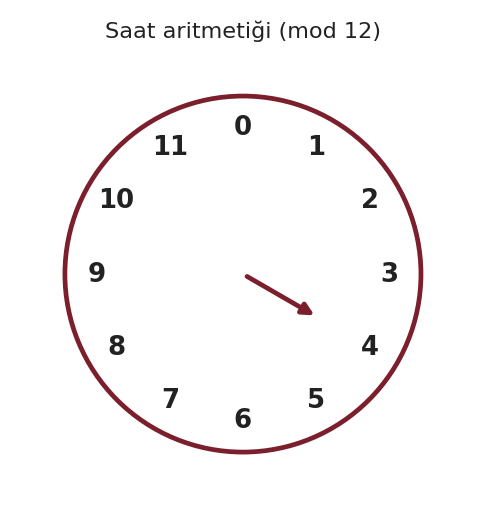
\includegraphics[width=0.56\linewidth]{figs/clock_mod.png}
\caption{Saat aritmetiği: mod 12 döngüsü.}
\end{figure}

\section{İleri Örnekler: Üs Alma, Ters Eleman ve Sistemler}

Kongrüansların gücü, büyük hesapları küçük döngülere indirgemesinde ortaya çıkar. Aşağıdaki örnekler modüler üs alma, ters eleman ve kongrüans sistemlerini gösterir.

\begin{tcolorbox}[bookbox,colback=cEx]\textbf{\textsf{\textcolor{cAcc}{Örnek.}}}\quad \textbf{Büyük üs. }10¹⁰⁰’ün 7’ye bölümünden kalan nedir? 10 ≡ 3 (mod 7) ve 3’ün kuvvetleri mod 7’de 3, 2, 6, 4, 5, 1 diye 6 adımda bir tekrarlar. 100 = 6·16 + 4 olduğundan 10¹⁰⁰ ≡ 3¹⁰⁰ ≡ 3⁴ ≡ 4 (mod 7). Kalan 4’tür — yüz basamaklı sayıyı hiç yazmadan.\end{tcolorbox}

\begin{tcolorbox}[bookbox,colback=cEx]\textbf{\textsf{\textcolor{cAcc}{Örnek.}}}\quad \textbf{11’e bölünebilme. }10 ≡ −1 (mod 11) olduğundan bir sayı, rakamlarının dönüşümlü (alternating) toplamına denktir. Örneğin 918082: 2 − 8 + 0 − 8 + 1 − 9 = −22 ≡ 0 (mod 11), yani 918082 sayısı 11’e bölünür.\end{tcolorbox}

\begin{tcolorbox}[bookbox,colback=cEx]\textbf{\textsf{\textcolor{cAcc}{Örnek.}}}\quad \textbf{Lineer kongrüans. }3x ≡ 4 (mod 5) çözülür: 3’ün mod 5 tersi 2’dir (çünkü 3·2 = 6 ≡ 1). İki tarafı 2 ile çarparsak x ≡ 8 ≡ 3 (mod 5). Denetim: 3·3 = 9 ≡ 4 ✓. Ters eleman ancak gcd(3, 5) = 1 olduğu için vardır.\end{tcolorbox}

\begin{tcolorbox}[bookbox,colback=cEx]\textbf{\textsf{\textcolor{cAcc}{Örnek.}}}\quad \textbf{Kongrüans sistemi (Çin Kalan Teoremi’nin önizlemesi). }x ≡ 2 (mod 3) ve x ≡ 3 (mod 5) sistemini sağlayan x, mod 15’te tek bir sınıftır: x ≡ 8 (mod 15). Denetim: 8 ≡ 2 (mod 3) ve 8 ≡ 3 (mod 5) ✓. Modüller aralarında asal olduğunda çözüm daima vardır ve çarpımları modunda tektir.\end{tcolorbox}

\begin{tcolorbox}[bookbox,colback=cMis]\textbf{\textsf{\textcolor{cAcc}{Yaygın Kavram Yanılgıları}}}\quad \textbf{“a ≡ b (mod n) ise a = b’dir.” — }Kongrüans eşitlik değildir; a ile b yalnızca aynı kalanı verir. 8 ≡ 3 (mod 5) doğrudur ama 8 ≠ 3.\par\medskip{}\textbf{“Kongrüansta her iki tarafı bölebilirim.” — }Sadeleştirme yalnızca bölünen sayı ile modül aralarında asalsa geçerlidir. 2·3 ≡ 2·0 (mod 6) iken 3 ≢ 0 (mod 6).\par\medskip{}\textbf{“aᵏ ≡ (a mod n)ᵏ’yı doğrudan hesaplarım, üssü de küçültürüm.” — }Taban mod n’e indirgenebilir, ama üs öyle indirgenemez; üs için kuvvetlerin döngüsü (ya da Euler teoremi) kullanılır.\par\medskip{}\textbf{“Her a’nın mod n tersi vardır.” — }Ters ancak gcd(a, n) = 1 iken vardır. Örneğin 2’nin mod 4 tersi yoktur.\par\medskip{}\textbf{“Negatif sayıların modu tanımsızdır.” — }Tanımlıdır: −3 ≡ 2 (mod 5), çünkü −3 + 5 = 2. Kalan daima 0 ile n − 1 arasında seçilir.\end{tcolorbox}

\section{Uygulama ve Eğitime Yansıma}

Modüler aritmetik gündelik teknolojinin görünmez altyapısıdır. Sağlama basamakları (ISBN, kredi kartlarında Luhn algoritması, TC kimlik numarası) hataları yakalamak için kongrüans kullanır; karma (hash) fonksiyonları ve rastgele sayı üreteçleri mod işlemiyle çalışır. En çarpıcı uygulama açık anahtarlı şifrelemedir (RSA): mesaj bir modül altında üs alınarak şifrelenir ve yalnızca ‘ters üssü’ bilen çözebilir.

Eğitim açısından modüler aritmetik, öğrenciye ‘eşitlik’ ile ‘denklik’ farkını en somut biçimde yaşatır ve soyut cebire (ℤₙ) yumuşak bir giriş sağlar. Saat aritmetiği ve haftanın günleri gibi tanıdık örnekler, konuyu günlük deneyime bağlayarak van Hiele düzeylerinde görsel/işlemsel düzeyden başlamayı kolaylaştırır.

\section{Yüksek Lisans Derinleştirmesi: ℤₙ Halkası ve Fermat–Euler}

Kongrüans sınıfları ℤₙ = \{[0], [1], …, [n − 1]\} kümesini oluşturur ve üzerindeki iyi tanımlı toplama–çarpma ile ℤₙ bir değişmeli halka olur. Bu halkanın çarpımsal tersi olan elemanları (birimler) tam olarak modülle aralarında asal olan sınıflardır; bunlar (ℤ/nℤ)* birimler grubunu oluşturur ve eleman sayısı Euler’in φ(n) fonksiyonuyla verilir. n asal olduğunda her sıfırdan farklı sınıfın tersi vardır, yani ℤₙ bir cisim (alan) olur.

Bu yapı iki klasik teoremi doğurur. Fermat’ın küçük teoremi: p asal ve gcd(a, p) = 1 ise aᵖ⁻¹ ≡ 1 (mod p). Onun genellemesi Euler teoremi: gcd(a, n) = 1 ise a\textasciicircum{}φ(n) ≡ 1 (mod n). Bu sonuçlar, ‘büyük üs’ örneğindeki döngüsel davranışın neden kaçınılmaz olduğunu açıklar: birimler grubunun sonlu olması, kuvvetlerin er geç tekrar 1’e dönmesini garanti eder.

RSA şifrelemesi tam da bu teoremlere dayanır: iki büyük asalın çarpımı n = pq alınır, şifreleme üssü e ve çözme üssü d, ed ≡ 1 (mod φ(n)) olacak biçimde seçilir; Euler teoremi sayesinde (mᵉ)ᵈ ≡ m (mod n) olur ve mesaj geri elde edilir. Güvenlik, n’i çarpanlarına ayırmanın (yani φ(n)’i bulmanın) pratikte çok zor olmasına dayanır. Böylece Bölüm~\ref{chap:kongruanslar}’nin soyut kongrüans cebri, doğrudan çağdaş güvenli iletişimin temeline bağlanır.

\section{Sayılar Kuramından Klasik Sonuçlar}

Kongrüans dili, sayılar kuramının pek çok klasik sonucunu erişilebilir kılar. Aşağıdaki örnekler bu gücü gösterir ve bölüm boyunca kurulan araçların nasıl bir araya geldiğini sergiler.

\begin{tcolorbox}[bookbox,colback=cEx]\textbf{\textsf{\textcolor{cAcc}{Örnek.}}}\quad \textbf{Euler φ hesabı. }φ(n), n ile aralarında asal olan 1 ≤ k ≤ n sayılarının adedidir. Örneğin φ(12) = 4 (bunlar 1, 5, 7, 11). Asal p için φ(p) = p − 1; aralarında asal m, n için φ(mn) = φ(m)φ(n). Bu fonksiyon, birimler grubunun büyüklüğünü verdiği için Euler teoreminin merkezindedir.\end{tcolorbox}

\begin{tcolorbox}[bookbox,colback=cEx]\textbf{\textsf{\textcolor{cAcc}{Örnek.}}}\quad \textbf{Çin Kalan Teoremi (tam çözüm). }x ≡ 2 (mod 3), x ≡ 3 (mod 5), x ≡ 2 (mod 7) sistemini çözelim. İlk iki denklik x ≡ 8 (mod 15) verir; buna x ≡ 2 (mod 7) eklenince x ≡ 23 (mod 105) bulunur. Denetim: 23 = 3·7 + 2, 23 = 4·5 + 3, 23 = 7·3 + 2. Modüller ikişer aralarında asal olduğundan çözüm, çarpımları olan 105 modunda tektir.\end{tcolorbox}

\begin{tcolorbox}[bookbox,colback=cEx]\textbf{\textsf{\textcolor{cAcc}{Örnek.}}}\quad \textbf{Wilson teoremi. }p asal ise (p − 1)! ≡ −1 (mod p). Örneğin p = 5 için 4! = 24 ≡ −1 (mod 5). Bu, bir sayının asallığını (verimsiz de olsa) kongrüansla sınayan zarif bir ölçüttür ve modüler çarpımın grup yapısını sergiler.\end{tcolorbox}

Dokuza atma (casting out nines), bu fikirlerin gündelik bir uygulamasıdır: bir çarpma işleminin doğruluğu, tarafların rakam toplamları mod 9’da karşılaştırılarak hızlıca sınanabilir; çünkü 10 ≡ 1 (mod 9), dolayısıyla her sayı rakam toplamına denktir. Bu yöntem her hatayı yakalamayı garanti etmez ama pek çok hatayı anında görünür kılar ve öğrenciye kongrüansın pratik değerini somutlaştırır.

Bu örnekler, Bölüm~\ref{chap:kongruanslar}’nin yalnızca soyut bir cebir alıştırması olmadığını ortaya koyar: Gauss’un icat ettiği dil, hem klasik sayılar kuramının derin teoremlerini hem de bilgisayar çağının şifreleme altyapısını taşıyacak kadar güçlüdür. Öğretmen adayı için buradaki ders, ‘saf’ ile ‘uygulamalı’ matematiğin çoğu zaman aynı fikrin iki yüzü olduğudur; kalanların basit aritmetiği, doğru ışıkta bakıldığında modern güvenli iletişimin temeline uzanır.

\section{Hızlı Üs Alma ve Bir RSA Örneği}

Modüler aritmetiğin pratik gücü, ‘tekrarlı kareleme’ (repeated squaring) yöntemiyle büyük üsleri hızla hesaplayabilmesinde ortaya çıkar. Fikir basittir: üssü ikili tabanda düşünüp tabanın karelerini birbiriyle çarparız; böylece n’inci kuvvet için n çarpma yerine yalnızca log₂n dolayında çarpma yeter.

\begin{tcolorbox}[bookbox,colback=cEx]\textbf{\textsf{\textcolor{cAcc}{Örnek.}}}\quad \textbf{Tekrarlı kareleme. }3¹³ mod 100 hesaplayalım. 13 = 8 + 4 + 1 olduğundan 3¹³ = 3⁸ · 3⁴ · 3¹. Kareleri sırayla bulalım: 3² = 9, 3⁴ = 81, 3⁸ = 81² = 6561 ≡ 61 (mod 100). Şimdi 3¹³ ≡ 61 · 81 · 3 (mod 100): 61 · 81 = 4941 ≡ 41, sonra 41 · 3 = 123 ≡ 23. Demek ki 3¹³ ≡ 23 (mod 100) — on üç çarpma yerine birkaç kareleme ile.\end{tcolorbox}

Bu yöntem, açık anahtarlı şifrelemenin (RSA) hesaplanabilir olmasının anahtarıdır: gerçek uygulamada üsler yüzlerce basamaklıdır ve yalnızca tekrarlı kareleme sayesinde makul sürede hesaplanır. Aşağıda RSA’nın çekirdek fikrini küçük sayılarla baştan sona izleyelim.

\begin{tcolorbox}[bookbox,colback=cEx]\textbf{\textsf{\textcolor{cAcc}{Örnek.}}}\quad \textbf{RSA (küçük örnek). }İki asal seçelim: p = 3, q = 11, böylece n = pq = 33 ve φ(n) = (p − 1)(q − 1) = 2 · 10 = 20. Şifreleme üssü olarak gcd(e, 20) = 1 sağlayan e = 3’ü alalım; çözme üssü d ise 3d ≡ 1 (mod 20) denkleminden d = 7’dir (çünkü 3 · 7 = 21 ≡ 1). Açık anahtar (n, e) = (33, 3), gizli anahtar (n, d) = (33, 7).\end{tcolorbox}

\begin{tcolorbox}[bookbox,colback=cEx]\textbf{\textsf{\textcolor{cAcc}{Örnek.}}}\quad \textbf{Şifreleme ve çözme. }m = 2 mesajını şifreleyelim: c = mᵉ mod n = 2³ = 8 (mod 33). Çözmek için c\textasciicircum{}d mod n = 8⁷ (mod 33) hesaplanır. Tekrarlı karelemeyle: 8² = 64 ≡ 31, 8⁴ ≡ 31² = 961 ≡ 4, dolayısıyla 8⁷ = 8⁴ · 8² · 8 ≡ 4 · 31 · 8 = 992 ≡ 2 (mod 33). Başlangıçtaki m = 2 mesajı geri elde edildi. ✓\end{tcolorbox}

Bu örnek RSA’nın neden çalıştığını da somutlaştırır: ed ≡ 1 (mod φ(n)) seçildiğinden, Euler teoremi (Bölüm~\ref{chap:kongruanslar}) gereği (mᵉ)ᵈ = m\textasciicircum{}\{ed\} ≡ m (mod n) olur. Güvenlik ise şuna dayanır: açık anahtardan (n, e) gizli anahtarı (d) bulmak için φ(n) gerekir; φ(n)’i bulmak da n’i asal çarpanlarına (p ve q) ayırmayı gerektirir. Küçük sayılarda bu kolaydır, ama yüzlerce basamaklı n için pratikte çözülemez zorluktadır.

Böylece Gauss’un iki yüzyıl önce icat ettiği kongrüans dili, bugün internetteki güvenli iletişimin (bankacılık, mesajlaşma, dijital imza) matematiksel temelini oluşturur. Öğretmen adayı için bu, ‘neden soyut sayılar kuramı öğreniyoruz?’ sorusuna verilebilecek en çarpıcı yanıtlardan biridir: en saf matematik, çoğu zaman en somut teknolojinin kalbinde yatar.

\begin{tcolorbox}[bookbox,colback=cDef]\textbf{\textsf{\textcolor{cAcc}{Tarihsel Not}}}\quad Carl Friedrich Gauss, kongrüans gösterimini içeren başyapıtı Disquisitiones Arithmeticae’yi 1801’de, henüz yirmi dört yaşındayken yayımladı. Eser, dağınık sayı-kuramı gözlemlerini tek bir sistemli çerçevede topladı ve modüler aritmetiği bağımsız bir disiplin hâline getirdi. İlginç bir tarihsel bağ: Fermat’ın küçük teoremi, Pierre de Fermat tarafından 1640’ta bir mektupta ispatsız dile getirilmiş, ilk yayımlanan ispatı ise Euler’den gelmiştir. Bu teorem, iki yüzyıl sonra RSA şifrelemesinin çekirdeği olacaktı.\end{tcolorbox}

\section{Modüler Aritmetiği Görmek: Döngüler ve Kontrol Basamakları}

Modüler aritmetikte kuvvetler ve katlar sonunda kendini tekrar eder; çünkü yalnızca sonlu sayıda kalan vardır. Bu tekrarı bir çember üzerinde çizmek, Fermat teoreminin ve ‘üreteç’ kavramının neden işlediğini sezdirir.

\begin{figure}[htbp]
\centering
\begin{tikzpicture}[v/.style={circle,draw=bar,fill=white,line width=.8pt,minimum size=6.5mm,font=\sffamily\small},>={Stealth[length=5pt]}]
\begin{scope}
\foreach \k in {0,...,6}{\node[v] (a\k) at ({90-360/7*\k}:1.6) {\k};}
\foreach \x/\y in {1/3,3/2,2/6,6/4,4/5,5/1}{\draw[->,acc,line width=.9pt] (a\x) to[bend left=12] (a\y);}
\draw[->,mid,line width=.8pt] (a0) edge[loop above,looseness=6] (a0);
\node[small lbl,anchor=north] at (0,-2.05) {$x\mapsto 3x \pmod 7$\\tek döngü: $1\to3\to2\to6\to4\to5\to1$};
\end{scope}
\begin{scope}[xshift=5.2cm]
\foreach \k in {0,...,6}{\node[v] (b\k) at ({90-360/7*\k}:1.6) {\k};}
\foreach \x/\y in {1/2,2/4,4/1}{\draw[->,warm,line width=.9pt] (b\x) to[bend left=12] (b\y);}
\foreach \x/\y in {3/6,6/5,5/3}{\draw[->,grn,line width=.9pt] (b\x) to[bend left=12] (b\y);}
\draw[->,mid,line width=.8pt] (b0) edge[loop above,looseness=6] (b0);
\node[small lbl,anchor=north] at (0,-2.05) {$x\mapsto 2x \pmod 7$\\iki döngü: $1\to2\to4\to1$ ve $3\to6\to5\to3$};
\end{scope}
\end{tikzpicture}
\caption{Mod 7’de 3 ile ve 2 ile çarpmanın kalanlar üzerindeki etkisi. 3 ile çarpma sıfırdan farklı altı kalanı tek bir döngüde dolaşır (3 bir \emph{üreteçtir}); 2 ile çarpma ise iki ayrı üçlü döngü oluşturur. Her iki durumda da döngü uzunluğu 6’yı böler — Fermat teoreminin ($a^{6}\equiv1$) görsel karşılığı.}
\end{figure}

\begin{table}[htbp]
\centering\small
\renewcommand{\arraystretch}{1.25}
\begin{tabular}{lcccccc}
\toprule
$k$ & 1 & 2 & 3 & 4 & 5 & 6\\
\midrule
$2^k \bmod 7$ & 2 & 4 & \textbf{1} & 2 & 4 & 1\\
$3^k \bmod 7$ & 3 & 2 & 6 & 4 & 5 & \textbf{1}\\
\bottomrule
\end{tabular}
\caption{Kuvvetlerin kalanları. 2’nin kuvvetleri 3 adımda, 3’ün kuvvetleri 6 adımda başa döner. Buradan örneğin $2^{100}=2^{3\cdot33+1}\equiv2 \pmod 7$ hemen okunur.}
\end{table}

\begin{ornek}[\textbf{Kontrol basamağı: ISBN-10.}]
Eski on haneli ISBN numaralarında $a_1a_2\cdots a_{10}$ rakamları için
\[
10a_1+9a_2+8a_3+\cdots+2a_9+1\cdot a_{10}\equiv0 \pmod{11}
\]
koşulu aranır; son hane bu koşulu sağlayacak biçimde seçilir (gerekirse 10 yerine ‘X’ yazılır). 0-306-40615-2 numarası için toplam
\[
0+27+0+42+24+0+24+3+10+2=132=12\cdot11\equiv0 \pmod{11}
\]
olduğundan numara geçerlidir. Neden 11? Tek bir rakam hatası toplamı $c\cdot d$ kadar değiştirir ($c$ ağırlık, $d$ hata); 11 asal ve $1\le c,d\le10$ olduğundan bu değişim 11’e bölünemez, hata mutlaka yakalanır. Komşu iki rakamın yer değiştirmesi de toplamı $\pm(a_i-a_{i+1})$ kadar değiştirir ve aynı nedenle yakalanır. Modülün asal olması, sıfır bölen bulunmaması demektir — aşağıdaki yanılgı kutusuyla karşılaştırın.
\end{ornek}

\begin{ornek}[\textbf{İki koşulu birden sağlamak.}]
3’e bölündüğünde 2, 5’e bölündüğünde 3 kalanını veren sayıları arayalım. $x\equiv3\pmod5$ koşulunu sağlayanlar $3,8,13,18,23,\dots$ dizisidir; bunların 3’e göre kalanları $0,2,1,0,2,\dots$ biçiminde döner. İlk uygun değer 8’dir ve 3 ile 5 aralarında asal olduğundan çözümler tam olarak $x\equiv8\pmod{15}$ sınıfıdır. Bu, \emph{Çin kalan teoreminin} en küçük örneğidir: aralarında asal modüller için eşzamanlı kongrüansların çözümü vardır ve çarpım modülüne göre tektir — varlık ve teklik sorularının modüler aritmetikteki biçimi.
\end{ornek}

\begin{yanilgi}[Yaygın Kavram Yanılgıları]
\textbf{‘$ab\equiv0$ ise $a\equiv0$ ya da $b\equiv0$’dır.’} — Mod 6’da $2\cdot3=6\equiv0$ ama ne 2 ne 3 sıfırdır. Bu özellik ancak modül asal olduğunda geçerlidir.

\smallskip
\textbf{‘Her iki tarafı aynı sayıya bölebilirim.’} — $2x\equiv2\pmod6$ kongrüansında 2’ye ‘bölerek’ $x\equiv1$ yazmak, $x=4$ çözümünü kaybettirir ($2\cdot4=8\equiv2$). Doğru kural: $\gcd(c,n)=d$ ise $cx\equiv cy\pmod n\iff x\equiv y\pmod{n/d}$; burada $x\equiv1\pmod3$.

\smallskip
\textbf{‘$a\equiv b\pmod n$ ise $2^a\equiv2^b\pmod n$’dir.’} — Üsler aynı modülde indirgenemez: $4\equiv1\pmod3$ ama $2^4=16\equiv1$, $2^1=2$. Üsler, kuvvetlerin döngü uzunluğuna göre indirgenir (Fermat–Euler).
\end{yanilgi}

\begin{sinif}[Sınıfta · Haftanın günü]
‘Bugün salı. 100 gün sonra hangi gün olur? $10^{10}$ gün sonra?’ Birinci soru $100\equiv2\pmod7$ ile kolayca çözülür. İkincisi için öğrenciler $10\equiv3\pmod7$ gözleminden sonra yukarıdaki $3^k$ tablosunu kullanarak $3^{10}=3^{6}\cdot3^4\equiv4\pmod7$ bulur: dört gün sonrası, yani cumartesi. Etkinlik, ‘sayıyı hesaplamadan kalanını bulmak’ fikrini — bölümün ana düşüncesini — somutlaştırır.
\end{sinif}

\section*{Alıştırmalar}

\reviewitem{1}{7¹⁰⁰ sayısının 5’e bölümünden kalanı bulun.}

\reviewitem{2}{3x ≡ 1 (mod 7) denklemini çözün ve 3’ün mod 7 tersini belirtin.}

\reviewitem{3}{Bir sayının 11’e bölünebilme kuralını, 10 ≡ −1 (mod 11) kongrüansını kullanarak gerekçelendirin.}

\reviewitem{4}{φ(36) değerini hesaplayın (çarpımsallık özelliğini kullanabilirsiniz).}

\reviewitem{5}{RSA örneğini p = 5, q = 11 ile tekrarlayın: n ve φ(n)’i bulun, uygun bir e seçin ve buna karşılık gelen d’yi hesaplayın.}

\section*{Bölüm Özeti}

\begin{itemize}\setlength{\itemsep}{2pt}\setlength{\parskip}{0pt}
\item a ≡ b (mod n) ⇔ n | (a − b); bir denklik bağıntısıdır.
\item Kongrüans toplama ve çarpma ile uyumludur; bu ℤₙ aritmetiğini kurar.
\item Bölünebilme kuralları ve döngüsel sayma kongrüansların uygulamalarıdır.
\end{itemize}

\section*{Gözden Geçirme Soruları}

\reviewitem{1}{7 | (a − b) uyumunu kullanarak 10¹⁰⁰’ün 7’ye bölümünden kalanı bulunuz (yaklaşımınızı açıklayın).}

\reviewitem{2}{Çıkarmanın da kongrüansla uyumlu olduğunu gösteriniz.}

\section*{Çoktan Seçmeli Sorular}

\mcqq{1}{a ≡ b (mod n) ne demektir?}

\mcqo{A}{a = b}

\mcqo{B}{n | (a − b)}

\mcqo{C}{a | (n − b)}

\mcqo{D}{b | (a − n)}

\mcqa{B}{a≡b (mod n): n, a−b’yi böler.}

\mcqq{2}{Kongrüans ℤ üzerinde ne tür bir bağıntıdır?}

\mcqo{A}{Sıralama}

\mcqo{B}{Denklik}

\mcqo{C}{Fonksiyon}

\mcqo{D}{Ters simetrik}

\mcqa{B}{Kongrüans ℤ üzerinde bir denklik bağıntısıdır.}

\mcqq{3}{9’a bölünebilme kuralı hangi kongrüansa dayanır?}

\mcqo{A}{10 ≡ 0 (mod 9)}

\mcqo{B}{10 ≡ 1 (mod 9)}

\mcqo{C}{9 ≡ 1 (mod 10)}

\mcqo{D}{10 ≡ −1 (mod 9)}

\mcqa{B}{10≡1 (mod 9) olduğundan sayı, rakam toplamına denktir.}

\mcqq{4}{17 ≡ ? (mod 5)}

\mcqo{A}{0}

\mcqo{B}{1}

\mcqo{C}{2}

\mcqo{D}{3}

\mcqa{C}{17 = 3·5 + 2, kalan 2.}

\mcqq{5}{a ≡ a′ ve b ≡ b′ (mod n) ise a + b ≡ ?}

\mcqo{A}{a′ + b′}

\mcqo{B}{a′ − b′}

\mcqo{C}{a′b′}

\mcqo{D}{a′}

\mcqa{A}{Toplama kongrüansla uyumludur: a+b ≡ a′+b′.}

\mcqq{6}{a ≡ a′ ve b ≡ b′ (mod n) ise a·b ≡ ?}

\mcqo{A}{a′ + b′}

\mcqo{B}{a − b}

\mcqo{C}{a′b′}

\mcqo{D}{0}

\mcqa{C}{Çarpma kongrüansla uyumludur: ab ≡ a′b′.}

\mcqq{7}{25 ≡ ? (mod 7)}

\mcqo{A}{1}

\mcqo{B}{2}

\mcqo{C}{3}

\mcqo{D}{4}

\mcqa{D}{25 = 3·7 + 4, kalan 4.}

\mcqq{8}{Kongrüansın yansıma özelliği (a ≡ a) neye dayanır?}

\mcqo{A}{n | a}

\mcqo{B}{n | 0}

\mcqo{C}{n | 1}

\mcqo{D}{a | n}

\mcqa{B}{a−a = 0 ve n|0 olduğundan a≡a.}

\mcqq{9}{−3 ≡ ? (mod 5)}

\mcqo{A}{−3}

\mcqo{B}{3}

\mcqo{C}{2}

\mcqo{D}{4}

\mcqa{C}{−3 + 5 = 2, yani −3 ≡ 2 (mod 5).}

\mcqq{10}{Bir sayının 3’e bölünebilmesi için ölçüt nedir?}

\mcqo{A}{Son rakamı 3’tür}

\mcqo{B}{Rakamları toplamı 3’e bölünür}

\mcqo{C}{Çifttir}

\mcqo{D}{Son iki rakamı 3’e bölünür}

\mcqa{B}{10≡1 (mod 3) olduğundan rakam toplamı 3 için de ölçüttür.}

\mcqq{11}{Saat aritmetiği hangi modda çalışır?}

\mcqo{A}{mod 7}

\mcqo{B}{mod 10}

\mcqo{C}{mod 12}

\mcqo{D}{mod 60}

\mcqa{C}{Saat, 12 modunda döngüseldir.}

\mcqq{12}{Haftanın günleri hangi modda döngüseldir?}

\mcqo{A}{mod 12}

\mcqo{B}{mod 7}

\mcqo{C}{mod 24}

\mcqo{D}{mod 30}

\mcqa{B}{Günler 7 modunda tekrarlanır.}

\mcqq{13}{ℤₙ neyi mümkün kılar?}

\mcqo{A}{Sonsuz işlem}

\mcqo{B}{Sonlu bir küme üzerinde tutarlı toplama ve çarpma}

\mcqo{C}{Sıralama}

\mcqo{D}{Her zaman bölme}

\mcqa{B}{İşlemlerle uyum, ℤₙ üzerinde tutarlı aritmetiği kurar.}

\mcqq{14}{Kongrüansın toplama ile uyumu neye dayanır?}

\mcqo{A}{Çarpmaya}

\mcqo{B}{n | (a − a′) ve n | (b − b′) ⇒ n | toplam farkı}

\mcqo{C}{Sıralamaya}

\mcqo{D}{Fermat teoremine}

\mcqa{B}{(a−a′)+(b−b′) farkının bölünmesi toplama uyumunu verir.}

\mcqq{15}{100 ≡ ? (mod 9)}

\mcqo{A}{0}

\mcqo{B}{1}

\mcqo{C}{2}

\mcqo{D}{9}

\mcqa{B}{100 = 11·9 + 1, kalan 1.}

\mcqq{16}{Fermat’ın küçük teoremi (p asal) ne der?}

\mcqo{A}{a\textasciicircum{}p ≡ 0 (mod p)}

\mcqo{B}{a\textasciicircum{}p ≡ a (mod p)}

\mcqo{C}{a ≡ p}

\mcqo{D}{a² ≡ 1 (mod p)}

\mcqa{B}{Fermat: p asalsa a\textasciicircum{}p ≡ a (mod p).}

\mcqq{17}{a ≡ b (mod n) ise a ve b’nin n’ye bölümünden kalanları nasıldır?}

\mcqo{A}{Farklıdır}

\mcqo{B}{Eşittir}

\mcqo{C}{Toplamı n’dir}

\mcqo{D}{Çarpımı 0’dır}

\mcqa{B}{Aynı sınıftaki sayılar aynı kalanı verir.}

\mcqq{18}{12 ≡ 0 (mod n) eşitliği aşağıdaki hangi n için doğrudur?}

\mcqo{A}{n = 5}

\mcqo{B}{n = 7}

\mcqo{C}{n = 3}

\mcqo{D}{n = 8}

\mcqa{C}{3 | 12 olduğundan 12 ≡ 0 (mod 3).}

\mcqq{19}{Kongrüans neden “yapı koruyan” bir muhakeme örneğidir?}

\mcqo{A}{Sayıları büyütür}

\mcqo{B}{Ayrıntıyı atarken toplama–çarpma yapısını korur}

\mcqo{C}{Yalnızca bilgi kaybettirir}

\mcqo{D}{İşe yaramaz}

\mcqa{B}{Ayrıntıyı atarken toplama-çarpma yapısını korur.}

\mcqq{20}{7 | (a − b) bağıntısında [0] denklik sınıfı nedir?}

\mcqo{A}{Tek sayılar}

\mcqo{B}{7’nin katları}

\mcqo{C}{Asal sayılar}

\mcqo{D}{Tüm ℤ}

\mcqa{B}{[0], farkı 7’ye bölünenler, yani 7’nin katlarıdır.}


\clearpage

\clearpage
\chapter{Fonksiyonlar}
\label{chap:fonksiyonlar}


\par\smallskip{\sffamily\bfseries\color{cAcc}Öğrenme Hedefleri}\nopagebreak

\begin{itemize}\setlength{\itemsep}{2pt}\setlength{\parskip}{0pt}
\item Fonksiyonu bağıntı olarak tanımlayabilme.
\item Birebir, örten ve eşleme kavramlarını ispatlarla kullanabilme.
\item Bileşke ve ters fonksiyonu kurabilme.
\end{itemize}

\section*{Bölüme Genel Bakış: Fonksiyon Kavramının Serüveni}

Bugün en temel sandığımız fonksiyon kavramı, aslında yüzyıllar süren bir olgunlaşmanın ürünüdür. On yedinci yüzyılda Leibniz ‘fonksiyon’ sözcüğünü bir eğriye bağlı büyüklükler için kullandı; on sekizinci yüzyılda Euler onu bir ‘analitik ifade’ (formül) olarak gördü. Dönüm noktası 1837’de Dirichlet ile geldi: fonksiyon, herhangi bir formüle bağlı olmaksızın ‘her girdiye bir çıktı atayan keyfi bir kural’ olarak tanımlandı. Yirminci yüzyılda Bourbaki bu fikri kümeler diline oturttu: fonksiyon, belirli bir koşulu sağlayan bir bağıntıdır.

Bu tarihsel yolculuk pedagojik olarak öğreticidir: öğrenciler de çoğu zaman fonksiyonu önce ‘formül’ olarak düşünür ve ‘kural’ ya da ‘küme’ görüşüne geçmekte zorlanır. Bu bölüm fonksiyonu bağıntı temelinde tanımlar, birebir/örten/eşleme ayrımını ispatlarla işler ve bileşke, ters, imge gibi işlemleri geliştirir; böylece öğrenci fonksiyonu bir işlem olarak olduğu kadar bir nesne olarak da görebilir hâle gelir.

\section{Tanım}

\begin{tcolorbox}[bookbox,colback=cDef]\textbf{\textsf{\textcolor{cAcc}{Tanım.}}}\quad f: A → B bir fonksiyon, her a ∈ A için tam olarak bir f(a) ∈ B belirleyen bir bağıntıdır. A tanım kümesi, B değer kümesi, f(A) = \{f(a): a ∈ A\} görüntüdür.\end{tcolorbox}

\section{Birebir, Örten, Eşleme}

\begin{tcolorbox}[bookbox,colback=cDef]\textbf{\textsf{\textcolor{cAcc}{Tanım.}}}\quad f birebirdir (injective): f(a₁) = f(a₂) ⇒ a₁ = a₂. f örtendir (surjective): her b ∈ B için f(a) = b olan bir a vardır. Hem birebir hem örten fonksiyon bir eşlemedir (bijection).\end{tcolorbox}

\begin{tcolorbox}[bookbox,colback=cEx]\textbf{\textsf{\textcolor{cAcc}{Örnek.}}}\quad f: ℝ → ℝ, f(x) = 2x + 3 bir eşlemedir.\par\medskip{}Birebir: 2x + 3 = 2y + 3 ⇒ x = y. Örten: verilen y için x = (y − 3)/2 seçilir, f(x) = y. Öyleyse f eşlemedir ve tersi f⁻¹(y) = (y − 3)/2. ∎\end{tcolorbox}

\begin{tcolorbox}[bookbox,colback=cEx]\textbf{\textsf{\textcolor{cAcc}{Örnek.}}}\quad f: ℤ → ℤ, f(n) = 2n birebirdir ama örten değildir (tek sayılar görüntüde yoktur). Bu, tanım ve değer kümesinin fonksiyonun kimliğinin parçası olduğunu gösterir.\end{tcolorbox}

\begin{tcolorbox}[bookbox,colback=cDep]\textbf{\textsf{\textcolor{cAcc}{Muhakeme/Felsefe Derinleştirmesi — Nesne olarak fonksiyon: tarihsel gelişim}}}\quad Fonksiyon kavramı önce ‘bir formül/eğri’ olarak düşünüldü; Dirichlet ile ‘her girdiye bir çıktı atayan keyfi kural’a, Bourbaki ile ‘belirli koşulları sağlayan bir bağıntı (küme)’ tanımına evrildi. Bu, matematiğin bir işlemi (dinamik) bir nesneye (statik küme) dönüştürerek üzerinde muhakeme edebilir kılışının örneğidir — matematikteki ‘varlık’ ve ‘inşa’ sorularının fonksiyonlara uygulanışıdır.\end{tcolorbox}

\begin{figure}[htbp]
\centering
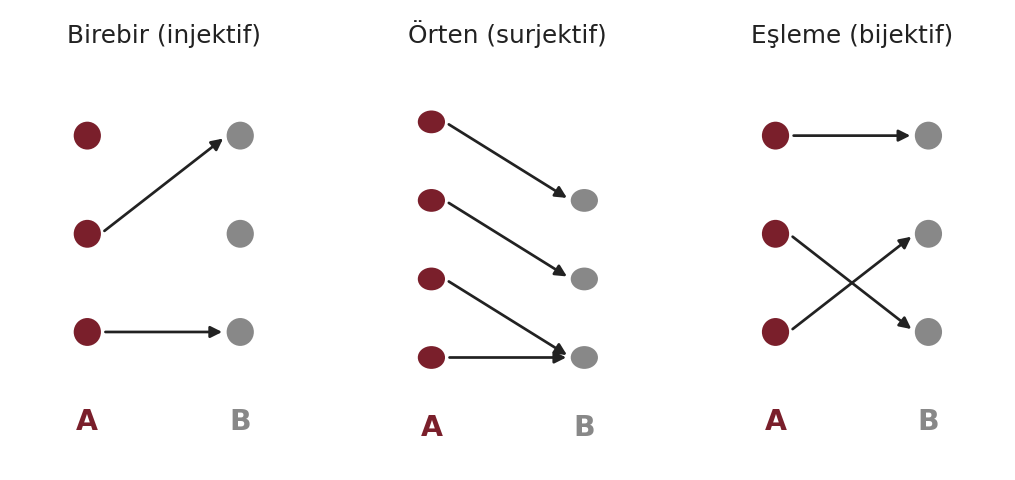
\includegraphics[width=0.91\linewidth]{figs/functions.png}
\caption{Birebir (injektif), örten (surjektif) ve eşleme (bijektif) fonksiyonlar.}
\end{figure}

\section{İleri Örnekler: Bileşke, Ters ve İmge}

Fonksiyon kavramını birkaç somut ispat ve hesapla derinleştirelim. Amaç, birebirlik ve örtenliğin nasıl gösterildiğini ve imge/ön imge kavramlarının nasıl çalıştığını görmektir.

\begin{tcolorbox}[bookbox,colback=cEx]\textbf{\textsf{\textcolor{cAcc}{Örnek.}}}\quad \textbf{Birebirlik ve örtenlik ispatı. }f: ℝ → ℝ, f(x) = x³ bir eşlemedir. Birebir: x³ = y³ ⇒ x = y (küp fonksiyonu kesin artandır). Örten: her y için x = ∛y seçilince f(x) = y. Bu yüzden tersi f⁻¹(y) = ∛y’dir. Buna karşılık f(x) = x² fonksiyonu ℝ → ℝ olarak ne birebirdir (f(−2) = f(2)) ne örtendir (negatif değerler görüntüde yok).\end{tcolorbox}

\begin{tcolorbox}[bookbox,colback=cEx]\textbf{\textsf{\textcolor{cAcc}{Örnek.}}}\quad \textbf{Bileşkenin sırası önemlidir. }f(x) = 2x + 3 ve g(x) = x² için (g ∘ f)(x) = (2x + 3)² iken (f ∘ g)(x) = 2x² + 3. İki bileşke farklıdır; bileşke işlemi genelde değişmeli değildir.\end{tcolorbox}

\begin{tcolorbox}[bookbox,colback=cEx]\textbf{\textsf{\textcolor{cAcc}{Örnek.}}}\quad \textbf{İmge ve ön imge. }f(x) = x² için f(\{−1, 0, 1, 2\}) = \{0, 1, 4\} (imge, tekrarları saymaz). Ön imge f⁻¹(\{4\}) = \{−2, 2\}; f⁻¹(\{−1\}) = ∅, çünkü hiçbir gerçek sayının karesi −1 değildir. Dikkat: burada f⁻¹ ters fonksiyon değil, küme ön imgesidir ve f birebir olmasa da tanımlıdır.\end{tcolorbox}

\begin{tcolorbox}[bookbox,colback=cEx]\textbf{\textsf{\textcolor{cAcc}{Örnek.}}}\quad \textbf{Güvercin yuvası ilkesi. }A ve B sonlu ve |A| > |B| ise A’dan B’ye birebir fonksiyon yoktur: en az iki farklı girdi aynı çıktıya gitmek zorundadır. Örneğin 13 kişiden en az ikisi aynı ayda doğmuştur (13 > 12). Bu basit gözlem, birebirliğin sonlu kümelerde boyutla doğrudan bağını gösterir.\end{tcolorbox}

\begin{tcolorbox}[bookbox,colback=cMis]\textbf{\textsf{\textcolor{cAcc}{Yaygın Kavram Yanılgıları}}}\quad \textbf{“f⁻¹, 1/f demektir.” — }f⁻¹ ters fonksiyondur, çarpımsal ters (1/f) değil. f(x) = 2x + 3 için f⁻¹(x) = (x − 3)/2’dir, 1/(2x + 3) değil.\par\medskip{}\textbf{“Her fonksiyonun tersi vardır.” — }Ters fonksiyon yalnızca eşlemeler (birebir ve örten) için tanımlıdır. Ancak küme ön imgesi f⁻¹(S) her fonksiyon için tanımlıdır.\par\medskip{}\textbf{“İmge ile değer kümesi aynıdır.” — }Görüntü (imge) f(A), değer kümesi B’nin bir alt kümesidir; eşit olması tam da örtenlik demektir.\par\medskip{}\textbf{“Tanım kümesini değiştirmek fonksiyonu değiştirmez.” — }Tanım ve değer kümesi fonksiyonun kimliğinin parçasıdır; x² fonksiyonu ℝ → ℝ ile [0,∞) → [0,∞) olarak farklı fonksiyonlardır (biri eşleme değil, diğeri eşleme).\par\medskip{}\textbf{“f(x + y) = f(x) + f(y) her fonksiyon için geçerlidir.” — }Bu yalnızca doğrusal (toplamsal) fonksiyonlar için doğrudur; f(x) = x² için f(1 + 1) = 4 ≠ f(1) + f(1) = 2.\end{tcolorbox}

\section{Uygulama ve Eğitime Yansıma}

Fonksiyon, hem matematiğin hem de bilgisayar biliminin merkezî kavramıdır: bir program fonksiyonu girdiyi çıktıya götüren bir eşlemedir; veri dönüşümleri, şifreleme (tek yönlü fonksiyonlar) ve makine öğrenmesi modelleri hep fonksiyon dilinde ifade edilir. Öğretimde en verimli köprü, fonksiyonu ‘girdi–çıktı makinesi’ olarak canlandırmak ve grafiğin ‘dikey doğru testi’yle (her girdiye tek çıktı) fonksiyon tanımını görselleştirmektir.

Öğrencilerin en sık zorlandığı nokta, birebirlik ile örtenliği ayırt etmek ve bunların tanım/değer kümesine bağlı olduğunu görmektir. ‘Yatay doğru testi’ (birebirlik) ile ‘dikey doğru testi’ (fonksiyon olma) ayrımını grafik üzerinde çalıştırmak, bu kavramları somutlaştırır ve öğrenciyi biçimsel ispata hazırlar.

\section{Yüksek Lisans Derinleştirmesi: Fonksiyon, Bağıntı ve Sayma}

Biçimsel olarak bir f: A → B fonksiyonu, A × B’nin özel bir alt kümesidir: her a ∈ A için tam olarak bir (a, b) çifti içeren bir bağıntı. Bu tanım, ‘fonksiyon bir kural mıdır yoksa bir nesne midir?’ tartışmasını kesin biçimde çözer — fonksiyon bir kümedir, dolayısıyla üzerinde matematiksel olarak konuşulabilecek bir nesnedir. Böylece Bölüm~\ref{chap:bagintilar}’in bağıntı çatısı, fonksiyonu da içine alır.

Fonksiyonlar aynı zamanda saymanın diliidir. Sonlu A, B için A’dan B’ye tüm fonksiyonların sayısı |B|\textasciicircum{}\{|A|\}’dır; bu yüzden fonksiyon uzayı çoğu zaman Bᴬ ile gösterilir. Özel bir durum, karakteristik fonksiyonlardır: A → \{0, 1\} fonksiyonları ile A’nın alt kümeleri birebir eşlenir (her alt küme, elemanlarına 1, diğerlerine 0 atayan fonksiyona karşılık gelir). Bu eşleme, |P(A)| = 2\textasciicircum{}\{|A|\} eşitliğinin kavramsal açıklamasıdır ve kuvvet kümesinin neden ‘2 üssü’ davrandığını gösterir.

Nihayet, birebir ve örten fonksiyonlar kardinalite karşılaştırmasının aracıdır (Bölüm~\ref{chap:kardinalite}): A’dan B’ye birebir fonksiyon varsa |A| ≤ |B|, bir eşleme varsa |A| = |B| deriz. Güvercin yuvası ilkesi bu dilin sonlu hâlidir; sonsuz kümelerde ise aynı fonksiyon dili, ‘bütün ile parçanın eş güçlü olabilmesi’ gibi sezgiye aykırı ama tutarlı sonuçlara götürür. Böylece fonksiyon kavramı, kümelerden kardinaliteye uzanan teknik omurganın taşıyıcı kirişidir.

\section{Eşlemeler, Permütasyonlar ve Tersler}

Fonksiyonların tersi ve bileşkesi zengin bir yapı kurar. Bir eşlemenin tersi tektir ve f⁻¹ ∘ f = id\_A ile f ∘ f⁻¹ = id\_B eşitliklerini sağlar. Eşleme olmayan fonksiyonlar için ise ‘tek yönlü’ tersler tanımlanabilir: f birebirse bir sol ters (g ∘ f = id\_A), örtense bir sağ ters (f ∘ h = id\_B) vardır. Bu ayrım, birebirlik ile örtenliğin cebirsel karşılığını verir.

\begin{tcolorbox}[bookbox,colback=cEx]\textbf{\textsf{\textcolor{cAcc}{Örnek.}}}\quad \textbf{Permütasyonlar. }Sonlu bir A kümesinin kendisine eşlemeleri, A’nın permütasyonlarıdır; |A| = n ise n! tane vardır. Permütasyonlar bileşke altında bir grup (simetrik grup Sₙ) oluşturur: birim permütasyon vardır, her permütasyonun tersi vardır ve bileşke birleşmelidir. Böylece fonksiyon kavramı doğrudan soyut cebre açılır.\end{tcolorbox}

\begin{tcolorbox}[bookbox,colback=cEx]\textbf{\textsf{\textcolor{cAcc}{Örnek.}}}\quad \textbf{Eşleştirme fonksiyonu. }Cantor’un eşleştirme fonksiyonu π(m, n) = (m + n)(m + n + 1)/2 + n, ℕ × ℕ’den ℕ’ye bir eşlemedir: iki doğal sayıyı tek bir doğal sayıya birebir kodlar. Bu, ‘iki boyutlu’ sayılabilir bilginin ‘tek boyuta’ sığdırılabileceğini gösterir ve Bölüm~\ref{chap:kardinalite}’teki ℕ × ℕ’nin sayılabilirliğinin somut kanıtıdır.\end{tcolorbox}

Kısıtlama (restriction) ve genişletme (extension) de fonksiyonlarla çalışmanın temel araçlarıdır: bir f: A → B fonksiyonu, A’nın bir alt kümesine kısıtlandığında yeni bir fonksiyon verir; tersine, bir fonksiyonu daha geniş bir tanım kümesine tutarlı biçimde genişletmek çoğu zaman matematiğin yaratıcı adımıdır (örneğin faktöriyelin gama fonksiyonuna genişletilmesi). Tüm bu işlemler, fonksiyonu edilgen bir ‘girdi–çıktı kuralı’ olmaktan çıkarıp üzerinde hesap yapılan bir nesneye dönüştürür.

Böylece fonksiyon, dersin teknik omurgasının taşıyıcı kirişidir: kümelerin (Bölüm~\ref{chap:kumeler}) ve bağıntıların (Bölüm~\ref{chap:bagintilar}) üzerine kurulur, kongrüans sınıflarında (Bölüm~\ref{chap:kongruanslar}) iyi tanımlılıkla iş görür ve kardinalite karşılaştırmasının (Bölüm~\ref{chap:kardinalite}) biricik aracıdır. Bu bağlantıları görmek öğrenciye, ayrı ayrı öğrenilen konuların aslında tek bir kavramsal ağın düğümleri olduğunu gösterir — matematiksel olgunluğun en önemli göstergelerinden biri de bu bütünlüğü görebilmektir.

\section{İmge ve Ön Görüntü Cebiri}

Fonksiyonlar yalnızca tek elemanları değil, tüm alt kümeleri de taşır: f, A’nın alt kümelerini B’nin alt kümelerine götürür (imge) ve tersine, B’nin alt kümelerinin ön görüntüsünü A’da belirler. Bu ‘küme düzeyindeki’ davranış, küme işlemleriyle (∪, ∩) ne kadar uyumlu olduğuna göre incelikli bir cebir kurar.

İmge, birleşimle tam uyumludur ama kesişimle yalnızca tek yönlü: f(A ∪ B) = f(A) ∪ f(B) her zaman doğrudur, oysa f(A ∩ B) ⊆ f(A) ∩ f(B) olur ve eşitlik genelde sağlanmaz. Bu asimetri, fonksiyonun ‘birleştirmeyi koruduğunu ama ayırt etmeyi kaybedebileceğini’ söyler.

\begin{tcolorbox}[bookbox,colback=cEx]\textbf{\textsf{\textcolor{cAcc}{Örnek.}}}\quad \textbf{Kesişimde eşitliğin bozulması. }f(x) = x², A = \{1\}, B = \{−1\} alalım. A ∩ B = ∅ olduğundan f(A ∩ B) = ∅. Ama f(A) = \{1\} ve f(B) = \{1\}, dolayısıyla f(A) ∩ f(B) = \{1\}. Görüldüğü gibi ∅ ⊊ \{1\}: eşitlik yok. Sebep açıktır — f birebir olmadığından farklı girdiler (1 ve −1) aynı çıktıya (1) gider ve kesişim ‘yapay olarak’ dolar. f birebir olsaydı eşitlik sağlanırdı.\end{tcolorbox}

Ön görüntü ise çok daha ‘uslu’dur: hem birleşimi hem kesişimi hem de tümleyeni korur. Yani f⁻¹(S ∪ T) = f⁻¹(S) ∪ f⁻¹(T), f⁻¹(S ∩ T) = f⁻¹(S) ∩ f⁻¹(T) ve f⁻¹(Sᶜ) = (f⁻¹(S))ᶜ. Bu düzenli davranış, ön görüntünün neden topoloji ve ölçü kuramında temel araç olduğunu açıklar: süreklilik ‘açık kümelerin ön görüntüsünün açık olması’, ölçülebilirlik ‘ölçülebilir kümelerin ön görüntüsünün ölçülebilir olması’ ile tanımlanır.

\begin{tcolorbox}[bookbox,colback=cEx]\textbf{\textsf{\textcolor{cAcc}{Örnek.}}}\quad \textbf{Ön görüntü kesişimi korur. }x ∈ f⁻¹(S ∩ T) ⇔ f(x) ∈ S ∩ T ⇔ f(x) ∈ S ∧ f(x) ∈ T ⇔ x ∈ f⁻¹(S) ∧ x ∈ f⁻¹(T) ⇔ x ∈ f⁻¹(S) ∩ f⁻¹(T). Her adım bir mantıksal eşdeğerlik olduğundan eşitlik kesindir; ön görüntünün üstünlüğü, tam da bu ‘⇔’ zincirinin hiç kırılmamasıdır. ∎\end{tcolorbox}

Gösterge (karakteristik) fonksiyonları bu resmi tamamlar. Bir A ⊆ U alt kümesinin gösterge fonksiyonu χ\_A, A’nın elemanlarına 1, diğerlerine 0 atar. Küme işlemleri bu fonksiyonların aritmetiğine çevrilir: χ\_\{A∩B\} = χ\_A · χ\_B ve χ\_\{A∪B\} = χ\_A + χ\_B − χ\_A · χ\_B. Böylece küme cebri, bir fonksiyon aritmetiğine dönüşür; bu, olasılık kuramında (bir olayın gösterge fonksiyonunun beklenen değeri, olasılığıdır) ve kombinatorikte sürekli kullanılan güçlü bir tekniktir.

Bu bölüm, fonksiyonun neden yalnızca ‘girdi–çıktı’ değil, aynı zamanda kümeler arası bir taşıyıcı olduğunu gösterir. İmge ve ön görüntünün farklı davranışları, birebirlik ve örtenlik kavramlarını yeni bir açıdan aydınlatır ve Bölüm~\ref{chap:kumeler}’un küme cebri ile Bölüm~\ref{chap:kardinalite}’ün kardinalite argümanlarını fonksiyon diliyle birbirine bağlar. Öğretmen adayı için buradaki incelik, ‘fonksiyon uygularken neyin korunup neyin kaybolduğunu’ bilmenin, ileri matematikteki pek çok tanımın (süreklilik, ölçülebilirlik) doğal olarak anlaşılmasını sağlamasıdır.

\begin{tcolorbox}[bookbox,colback=cDef]\textbf{\textsf{\textcolor{cAcc}{Tarihsel Not}}}\quad Fonksiyon kavramının modern tanımı, 1837’de Peter Gustav Lejeune Dirichlet ile netleşti: bir fonksiyon, herhangi bir formüle bağlı olmaksızın ‘her girdiye tam bir çıktı atayan’ kuraldır. Dirichlet, bunu göstermek için ünlü örneğini verdi — rasyonel sayılarda 1, irrasyonellerde 0 değerini alan, hiçbir formülle yazılamayan ama tümüyle geçerli bir fonksiyon. Bu ‘keyfi kural’ görüşü, fonksiyonu bir eğri ya da cebirsel ifadeyle özdeşleştiren eski anlayışı geride bıraktı ve modern analize giden yolu açtı.\end{tcolorbox}

\section{Fonksiyonları Görmek: Ok Diyagramları, Grafikler ve Tersler}

Bir fonksiyon üç farklı biçimde temsil edilebilir: bir kural (formül), bir ok diyagramı (sonlu kümelerde) ve bir grafik (reel fonksiyonlarda). Birebirlik, örtenlik, bileşke ve ters kavramlarının her biri bu temsillerin birinde çok daha kolay görülür. İyi bir öğretim, öğrencinin temsiller arasında rahatça geçiş yapabilmesini hedefler.

\begin{figure}[htbp]
\centering
\begin{tikzpicture}[e/.style={circle,fill=bar,inner sep=1.3pt},>={Stealth[length=5pt]}]
\foreach \x/\n/\lab/\k/\col in {0/A/{a_1,a_2,a_3}/3/acc,2.6/B/{b_1,b_2,b_3,b_4}/4/warm,5.2/C/{c_1,c_2,c_3}/3/grn}{
  \draw[\col,line width=.9pt,fill=\col!8] (\x,0) ellipse (.6 and 1.45);
  \node[font=\sffamily\bfseries\small,text=\col] at (\x,1.75) {$\n$};
  \foreach \t [count=\i] in \lab {\pgfmathsetmacro{\yy}{((\k+1)/2-\i)*0.72}\node[e] (\n\i) at (\x,\yy) {}; \node[font=\scriptsize,anchor=east] at (\x-.08,\yy) {$\t$};}
}
\foreach \a/\b in {1/1,2/3,3/4}{\draw[->,acc,line width=.8pt] (A\a)--(B\b);}
\foreach \a/\b in {1/1,2/1,3/2,4/3}{\draw[->,warm,line width=.8pt] (B\a)--(C\b);}
\node[font=\sffamily\small,text=acc] at (1.3,-1.85) {$f$ (birebir, örten değil)};
\node[font=\sffamily\small,text=warm] at (3.9,-1.85) {$g$ (örten, birebir değil)};
\draw[->,bar,line width=.9pt] (0,-2.35) to[bend right=14] node[below,font=\sffamily\small]{$g\circ f$: $a_1\mapsto c_1,\ a_2\mapsto c_2,\ a_3\mapsto c_3$ (bir eşleme!)} (5.2,-2.35);
\end{tikzpicture}
\caption{Ok diyagramlarıyla bileşke. $f$ birebir ama $b_2$’ye ok gelmediğinden örten değildir; $g$ örtendir ama $b_1$ ve $b_2$’yi aynı yere götürür. Buna rağmen $g\circ f$ bir eşlemedir: bileşenlerin kusurları birbirini ‘götürebilir’. $g\circ f$’nin birebir olması $f$’nin, örten olması ise $g$’nin karşılık gelen özelliğini zorunlu kılar (Alıştırma 4).}
\end{figure}

\begin{figure}[htbp]
\centering
\begin{tikzpicture}
\begin{axis}[width=.62\linewidth,height=.62\linewidth,xmin=-2.2,xmax=4.2,ymin=-2.2,ymax=4.2,axis lines=middle,
  xlabel={$x$},ylabel={$y$},tick label style={font=\sffamily\scriptsize},samples=120,
  legend style={at={(0.03,0.97)},anchor=north west,font=\sffamily\scriptsize,fill=white,draw=none}]
\addplot[acc,line width=1.2pt,domain=-2.2:1.43]{exp(x)}; \addlegendentry{$y=e^x$}
\addplot[warm,line width=1.2pt,domain=0.11:4.2]{ln(x)}; \addlegendentry{$y=\ln x$}
\addplot[mid,dashed,domain=-2.2:4.2]{x}; \addlegendentry{$y=x$}
\addplot[only marks,mark=*,mark size=1.6pt,acc] coordinates {(1,2.718)};
\addplot[only marks,mark=*,mark size=1.6pt,warm] coordinates {(2.718,1)};
\draw[dotted,bar] (axis cs:1,2.718)--(axis cs:2.718,1);
\end{axis}
\end{tikzpicture}
\caption{Bir eşleme ile tersinin grafikleri $y=x$ doğrusuna göre birbirinin yansımasıdır: $(1,e)$ noktası $(e,1)$ noktasına gider. Yatay her doğru $e^x$ grafiğini en fazla bir kez kestiği için $e^x$ birebirdir; ama $y\le0$ doğrularını hiç kesmediğinden $\mathbb R\to\mathbb R$ olarak örten değildir. Ters, ancak değer kümesi $(0,\infty)$ alındığında tanımlıdır.}
\end{figure}

\begin{ornek}[\textbf{Fonksiyonları saymak.}]
$|A|=3$, $|B|=4$ olsun. $A$’nın her elemanı için 4 seçenek olduğundan $4^3=64$ fonksiyon vardır. Birebir olanlarda seçenekler her adımda bir azalır: $4\cdot3\cdot2=24$. Örten fonksiyon yoktur, çünkü üç elemanlı bir küme dört elemanın hepsine ulaşamaz. Ters yönde $|A|=4$, $|B|=3$ için $3^4=81$ fonksiyonun kaçının örten olduğunu içerme–dışlama (Bölüm~\ref{chap:kumeler}) verir: bir elemanı ıskalayan fonksiyonlar $3\cdot2^4$, iki elemanı ıskalayanlar $3\cdot1^4$ olduğundan örten fonksiyon sayısı $81-48+3=36$’dır. Sayma sonuçları, sonlu kümelerde ‘birebir $\Rightarrow |A|\le|B|$’ ve ‘örten $\Rightarrow |A|\ge|B|$’ ilkelerinin nicel yüzüdür; bu ilkeler Bölüm~\ref{chap:kardinalite}’te sonsuz kümelerin karşılaştırılmasının tanımı olacaktır.
\end{ornek}

\begin{yanilgi}[Yaygın Kavram Yanılgıları]
\textbf{‘$f^{-1}(x)=\dfrac1{f(x)}$’dir.’} — Ters fonksiyon ile çarpımsal ters farklıdır. $f(x)=2x$ için $f^{-1}(x)=x/2$, ama $1/f(x)=1/(2x)$’tir. Gösterimdeki $-1$ üssü iki farklı işlem için kullanılır.

\smallskip
\textbf{‘$f^{-1}(D)$ yazabilmek için $f$ tersinir olmalıdır.’} — Ön görüntü $f^{-1}(D)=\{x: f(x)\in D\}$ her fonksiyon için tanımlıdır. $f(x)=x^2$ için $f^{-1}(\{4\})=\{-2,2\}$ ve $f^{-1}(\{-1\})=\varnothing$’dir; oysa ters fonksiyon yoktur.

\smallskip
\textbf{‘Her formül bir fonksiyon tanımlar.’} — $y^2=x$ bağıntısı her $x>0$’a iki $y$ karşılık getirdiğinden ($x$’ten $y$’ye) bir fonksiyon değildir; ‘dikey doğru testi’ bu kusuru grafikte gösterir. Tanım kümesi ve değer kümesi belirtilmeden ‘fonksiyon’ sözü eksiktir.

\smallskip
\textbf{‘$(g\circ f)^{-1}=g^{-1}\circ f^{-1}$’dir.’} — Sıra ters çevrilir: $(g\circ f)^{-1}=f^{-1}\circ g^{-1}$. Önce giyilen çorap, en son çıkarılır.
\end{yanilgi}

\begin{sinif}[Sınıfta · Üç temsil, bir fonksiyon]
Gruplara aynı fonksiyonun üç temsilinden yalnızca birini verin (formül, ok diyagramı ya da grafik) ve diğer ikisini kurmalarını isteyin. Ardından her grup, ‘Birebir mi? Örten mi? Tersi var mı?’ sorularını kendi başlangıç temsilinde yanıtlasın ve hangi temsilde yanıtın en kolay görüldüğünü tartışsın. Tipik bulgu: birebirlik grafikte (yatay doğru testi), örtenlik ok diyagramında (ok gelmeyen eleman), ters ise formülde (denklemi $x$ için çözme) daha kolay görülür.
\end{sinif}

\section*{Alıştırmalar}

\reviewitem{1}{f: ℝ → (−1, 1), f(x) = x / (1 + |x|) fonksiyonunun bir eşleme olduğunu gösterin ve tersini bulun.}

\reviewitem{2}{|A| = |B| = n (sonlu) ise, birebir bir f: A → B fonksiyonunun aynı zamanda örten olduğunu gösterin.}

\reviewitem{3}{Herhangi bir f: A → B ve alt kümeler için f(A₁ ∪ A₂) = f(A₁) ∪ f(A₂) eşitliğini kanıtlayın.}

\reviewitem{4}{g ∘ f bileşkesi birebirse, f’nin de birebir olduğunu gösterin. Aynı koşulda g birebir olmak zorunda mıdır?}

\reviewitem{5}{İki küme için χ\_\{A △ B\} = χ\_A + χ\_B (mod 2) olduğunu gösterin.}

\section*{Bölüm Özeti}

\begin{itemize}\setlength{\itemsep}{2pt}\setlength{\parskip}{0pt}
\item Fonksiyon, her girdiye tek çıktı atayan özel bir bağıntıdır.
\item Birebir/örten/eşleme ayrımı, fonksiyonun tersinin var olup olmadığını belirler.
\item Tanım ve değer kümesi fonksiyonun kimliğinin parçasıdır.
\end{itemize}

\section*{Gözden Geçirme Soruları}

\reviewitem{1}{f(x) = x² fonksiyonunun ℝ → ℝ ve [0, ∞) → [0, ∞) tanımlarında birebir/örtenlik durumunu karşılaştırınız.}

\reviewitem{2}{İki birebir fonksiyonun bileşkesinin de birebir olduğunu ispatlayınız.}

\section*{Çoktan Seçmeli Sorular}

\mcqq{1}{f(a₁) = f(a₂) ⇒ a₁ = a₂ koşulu neyi tanımlar?}

\mcqo{A}{Örten}

\mcqo{B}{Birebir}

\mcqo{C}{Sabit}

\mcqo{D}{Eşleme}

\mcqa{B}{Bu koşul birebirliğin (injektifliğin) tanımıdır.}

\mcqq{2}{Bir fonksiyonun tersinin var olması için gereken nedir?}

\mcqo{A}{Yalnızca birebir}

\mcqo{B}{Yalnızca örten}

\mcqo{C}{Eşleme (birebir ve örten)}

\mcqo{D}{Sürekli olması}

\mcqa{C}{Ters, ancak eşleme (birebir ve örten) fonksiyonda vardır.}

\mcqq{3}{f: ℤ → ℤ, f(n) = 2n için hangisi doğrudur?}

\mcqo{A}{Birebir, örten değil}

\mcqo{B}{Örten, birebir değil}

\mcqo{C}{Eşleme}

\mcqo{D}{Sabit}

\mcqa{A}{2n birebirdir ama tek sayılar görüntüde yok: örten değil.}

\mcqq{4}{Fonksiyon nasıl tanımlanır?}

\mcqo{A}{Her girdiye en az bir çıktı}

\mcqo{B}{Her girdiye tam bir çıktı}

\mcqo{C}{Her çıktıya bir girdi}

\mcqo{D}{Herhangi bir bağıntı}

\mcqa{B}{Fonksiyon her girdiye tam bir çıktı atar.}

\mcqq{5}{Örten (surjective) fonksiyon nedir?}

\mcqo{A}{f(a₁)=f(a₂) ⇒ a₁=a₂}

\mcqo{B}{Her b ∈ B için f(a) = b olan bir a vardır}

\mcqo{C}{Sabit fonksiyon}

\mcqo{D}{İkili bağıntı}

\mcqa{B}{Örtenlik: her hedef değere ulaşan bir girdi vardır.}

\mcqq{6}{f: ℝ → ℝ, f(x) = 2x + 3 nedir?}

\mcqo{A}{Yalnızca birebir}

\mcqo{B}{Yalnızca örten}

\mcqo{C}{Eşleme}

\mcqo{D}{Sabit}

\mcqa{C}{2x+3 hem birebir hem örten: eşleme.}

\mcqq{7}{f: ℝ → ℝ, f(x) = x² nedir?}

\mcqo{A}{Birebir}

\mcqo{B}{Örten}

\mcqo{C}{Eşleme}

\mcqo{D}{Ne birebir ne örten}

\mcqa{D}{x² ℝ’de ne birebir (±) ne örtendir (negatifler yok).}

\mcqq{8}{İki birebir fonksiyonun bileşkesi nasıldır?}

\mcqo{A}{Birebirdir}

\mcqo{B}{Örtendir}

\mcqo{C}{Sabittir}

\mcqo{D}{Tanımsızdır}

\mcqa{A}{Birebir fonksiyonların bileşkesi birebirdir.}

\mcqq{9}{f: A → B fonksiyonunda B neye karşılık gelir?}

\mcqo{A}{Görüntü}

\mcqo{B}{Değer kümesi}

\mcqo{C}{Çekirdek}

\mcqo{D}{Grafik}

\mcqa{B}{B, fonksiyonun değer kümesidir.}

\mcqq{10}{Görüntü kümesi f(A) nedir?}

\mcqo{A}{A}

\mcqo{B}{\{f(a): a ∈ A\}}

\mcqo{C}{B}

\mcqo{D}{∅}

\mcqa{B}{Görüntü, \{f(a): a∈A\} kümesidir.}

\mcqq{11}{f(x) = x², [0, ∞) → [0, ∞) olarak nedir?}

\mcqo{A}{Birebir değil}

\mcqo{B}{Örten değil}

\mcqo{C}{Eşleme}

\mcqo{D}{Sabit}

\mcqa{C}{Tanım/değer kümesi kısıtlanınca x² bir eşleme olur.}

\mcqq{12}{f birebir değilse ne olur?}

\mcqo{A}{Örten olur}

\mcqo{B}{Tersi (fonksiyon olarak) tanımlanamaz}

\mcqo{C}{Sabit olur}

\mcqo{D}{Sürekli olur}

\mcqa{B}{Birebir değilse ters tek değerli olmaz, tanımlanamaz.}

\mcqq{13}{f: \{1,2,3\} → \{a,b\} bir fonksiyon örten olabilir mi?}

\mcqo{A}{Evet ama birebir olamaz}

\mcqo{B}{Hayır}

\mcqo{C}{Yalnızca birebir olabilir}

\mcqo{D}{Hiçbiri}

\mcqa{A}{3 > 2 olduğundan örten olabilir ama birebir olamaz.}

\mcqq{14}{Bileşke (g ∘ f)(x) neye eşittir?}

\mcqo{A}{f(g(x))}

\mcqo{B}{g(f(x))}

\mcqo{C}{f(x)·g(x)}

\mcqo{D}{f(x)+g(x)}

\mcqa{B}{Bileşke önce f sonra g: g(f(x)).}

\mcqq{15}{Fonksiyon bir bağıntı olarak nasıl görülür?}

\mcqo{A}{Her a için birden çok (a, b)}

\mcqo{B}{Her a için tam bir (a, b) içerir}

\mcqo{C}{Bağıntı değildir}

\mcqo{D}{Simetriktir}

\mcqa{B}{Fonksiyon, her a için tek (a,b) içeren bağıntıdır.}

\mcqq{16}{Sabit fonksiyon f(x) = c genelde nasıldır?}

\mcqo{A}{Eşleme}

\mcqo{B}{Birebir}

\mcqo{C}{Genelde ne birebir ne örten}

\mcqo{D}{Örten}

\mcqa{C}{Sabit fonksiyon genelde ne birebir ne örtendir.}

\mcqq{17}{f bir eşleme ise sonlu A ve B için hangisi doğrudur?}

\mcqo{A}{|A| < |B|}

\mcqo{B}{|A| = |B|}

\mcqo{C}{|A| > |B|}

\mcqo{D}{İlişkisiz}

\mcqa{B}{Sonlu kümeler arası eşleme boyutları eşitler.}

\mcqq{18}{Ters fonksiyon f⁻¹ ne yapar?}

\mcqo{A}{A’dan A’ya gider}

\mcqo{B}{B’den A’ya gider; f(a)=b ⇒ f⁻¹(b)=a}

\mcqo{C}{f ile aynıdır}

\mcqo{D}{Sabittir}

\mcqa{B}{f⁻¹, çıktıyı girdisine geri gönderir.}

\mcqq{19}{f: ℤ → ℤ, f(n) = n + 1 nedir?}

\mcqo{A}{Birebir değil}

\mcqo{B}{Örten değil}

\mcqo{C}{Eşleme}

\mcqo{D}{Sabit}

\mcqa{C}{n+1 hem birebir hem örten: eşleme.}

\mcqq{20}{Fonksiyon kavramı tarihsel olarak (Dirichlet) nasıl gelişti?}

\mcqo{A}{Yalnızca formül olarak kaldı}

\mcqo{B}{Keyfi bir atama kuralına genişledi}

\mcqo{C}{Yalnızca eğri olarak}

\mcqo{D}{Hiç değişmedi}

\mcqa{B}{Dirichlet ile fonksiyon ‘keyfi atama kuralı’na genişledi.}


\clearpage

\clearpage
\chapter{Kardinalite ve Sonsuzluk}
\label{chap:kardinalite}


\par\smallskip{\sffamily\bfseries\color{cAcc}Öğrenme Hedefleri}\nopagebreak

\begin{itemize}\setlength{\itemsep}{2pt}\setlength{\parskip}{0pt}
\item Eş güçlülüğü eşleme üzerinden tanımlayabilme.
\item ℕ, ℤ, ℚ’nün sayılabilir, ℝ’nin sayılamaz olduğunu gerekçelendirebilme.
\item Sonlu–sonsuz ayrımının felsefi boyutunu tartışabilme.
\end{itemize}

\section*{Bölüme Genel Bakış: Sonsuzu Saymak}

Sonsuzluk, matematiğin en eski ve en sarsıcı kavramıdır. Galileo, on yedinci yüzyılda tam karelerin (1, 4, 9, …) tüm doğal sayılarla birebir eşlenebildiğini fark etti; ‘parça, bütün kadar çok’ görünüyordu ve bu sezgiyle çeliştiği için Galileo, sonsuzların karşılaştırılamayacağı sonucuna vardı. İki yüzyıl sonra Bernard Bolzano bu paradoksları yeniden ele aldı; ama asıl atılımı Georg Cantor yaptı: 1874 ve 1891’de sonsuz kümelerin farklı ‘büyüklüklere’ sahip olabileceğini kesin biçimde kanıtladı. Richard Dedekind ise sonsuz kümeyi tam da bu şaşırtıcı özellikle tanımladı: bir küme, öz bir alt kümesiyle eş güçlüyse sonsuzdur.

Bu bölüm, sonsuzu bir sezgi olmaktan çıkarıp üzerinde kesin teoremler kanıtlanan bir nesneye dönüştüren Cantor programını izler. Eş güçlülük, sayılabilirlik ve köşegen argümanı aracılığıyla ‘bazı sonsuzların diğerlerinden büyük olduğu’ sonucuna varırız. Öğretmen adayı için bu konu, hem matematiksel titizliğin zaferini hem de sezginin sınırlarını bir arada gösteren güçlü bir örnektir ve dersin tüm teknik omurgasını bir doruğa taşır.

\section{Eş Güçlülük}

\begin{tcolorbox}[bookbox,colback=cDef]\textbf{\textsf{\textcolor{cAcc}{Tanım.}}}\quad A ile B eş güçlüdür (|A| = |B|), aralarında bir eşleme varsa. Bir küme sayılabilir sonsuzdur, ℕ ile eş güçlüyse; sayılamazdır, sonsuz olup ℕ ile eş güçlü değilse.\end{tcolorbox}

\section{Sayılabilir Kümeler}

ℤ sayılabilirdir: 0, 1, −1, 2, −2, … sıralaması ℕ ile bir eşleme verir. ℚ da sayılabilirdir; kesirler bir tablo hâlinde dizilip köşegen yöntemiyle tek sıraya konabilir. Bu, ‘sonsuzun sonsuzu’ görünen ℚ’nün aslında ℕ kadar çok olduğunu gösterir.

\section{ℝ Sayılamaz: Cantor Köşegeni}

Köşegen argümanı tarihsel olarak küme kuramı paradokslarına giden yolun da bir durağıdır: Russell, paradoksuna Cantor’un ‘en büyük kardinal yoktur’ ispatını incelerken ulaşmıştır. Bu bölümde aynı fikri ondalık açılımlar üzerinde tam bir ispat olarak yazıyor ve eş güçlülüğün genel kuramına yerleştiriyoruz.

\begin{tcolorbox}[bookbox,colback=cDef]\textbf{\textsf{\textcolor{cAcc}{Teorem.}}}\quad (0, 1) aralığı sayılamazdır.\end{tcolorbox}

\begin{tcolorbox}[bookbox,colback=cEx]\textbf{\textsf{\textcolor{cAcc}{Örnek.}}}\quad İspat fikri (köşegen): (0,1)’in sayılabilir olduğunu, yani tüm ondalık açılımların bir listeye dizildiğini varsayalım. Köşegendeki i’nci basamağı değiştirerek yeni bir d sayısı kuralım (her basamağı listedeki i’nci sayının i’nci basamağından farklı seçelim). d, listedeki her sayıdan en az bir basamakta farklı olduğundan listede yer alamaz — çelişki. Öyleyse böyle bir liste yoktur; (0,1) sayılamaz. ∎\end{tcolorbox}

Aynı köşegen fikri genelleşir: her A kümesi için |A| < |P(A)| (Cantor teoremi). Böylece sonsuzun tek bir büyüklüğü değil, sonsuz bir hiyerarşisi vardır.

\begin{tcolorbox}[bookbox,colback=cDep]\textbf{\textsf{\textcolor{cAcc}{Muhakeme/Felsefe Derinleştirmesi — Edimsel ve olası sonsuzluk; Hilbert Oteli}}}\quad Aristo’dan beri süregelen ayrım, sonsuzun ‘tamamlanmış bir bütün’ (edimsel) mi yoksa yalnızca ‘hep daha ileri gidebilme’ (olası) mi olduğudur. Cantor’un eş güçlülük kuramı, edimsel sonsuzu matematiğin meşru bir nesnesi hâline getirdi — ve bu, dersin başında gördüğümüz temellendirme bunalımlarının merkezindeydi. Hilbert’in ‘sonsuz odalı oteli’ (dolu otel yeni konuğu, hatta sonsuz konuğu ağırlayabilir), sayılabilir sonsuzun sonlu sezgiyi nasıl kırdığını gösterir. Süreklilik hipotezi — ℕ ile ℝ arasında bir kardinalite olup olmadığı — ise ZFC’den bağımsızdır: aksiyomatik yöntemin sınırlarına dair somut bir örnektir.\end{tcolorbox}

\begin{figure}[htbp]
\centering
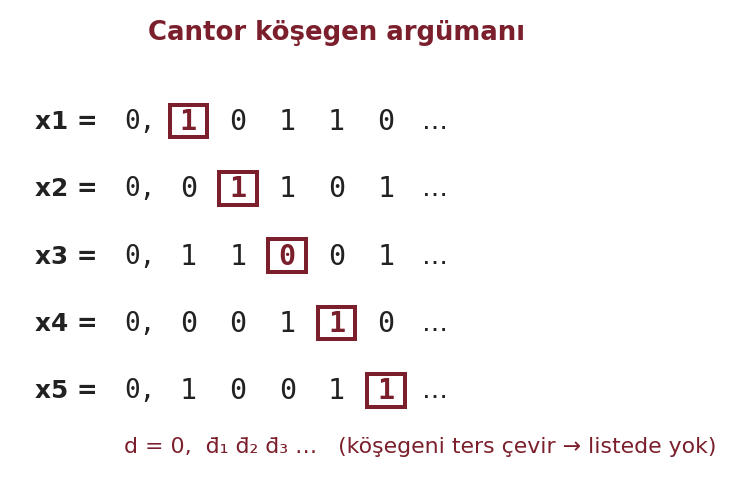
\includegraphics[width=0.80\linewidth]{figs/cantor.png}
\caption{Cantor köşegen argümanı: köşegen değiştirilerek listede olmayan bir sayı kurulur.}
\end{figure}

\section{İleri Örnekler: Eşlemeler ve Köşegen}

Sonsuz kümeleri karşılaştırmak, somut eşlemeler kurmayı ve köşegen argümanını ayrıntılı izlemeyi gerektirir. Aşağıdaki örnekler sayılabilirliğin sınırını ve sayılamazlığın kanıtını netleştirir.

\begin{tcolorbox}[bookbox,colback=cEx]\textbf{\textsf{\textcolor{cAcc}{Örnek.}}}\quad \textbf{Aralık ile tüm doğru eş güçlüdür. }f: (0, 1) → ℝ, f(x) = tan(π(x − ½)) bir eşlemedir: x, 0’dan 1’e giderken π(x − ½) açısı −π/2’den π/2’ye gider ve tan bu aralıkta tüm ℝ’yi birebir tarar. Demek ki minik bir açık aralık, tüm gerçel doğruyla aynı ‘büyüklüktedir’ — sonsuzda uzunluk sezgisi çöker.\end{tcolorbox}

\begin{tcolorbox}[bookbox,colback=cEx]\textbf{\textsf{\textcolor{cAcc}{Örnek.}}}\quad \textbf{ℚ sayılabilirdir. }Pozitif kesirler p/q, satırları pay ve sütunları payda olan sonsuz bir tabloya yerleştirilip köşegenler boyunca (tekrarları atlayarak) tek bir diziye dizilebilir: 1/1, 2/1, 1/2, 1/3, 2/2(atlanır), 3/1, … Negatifler ve sıfır da araya serpiştirilince ℚ ile ℕ arasında bir eşleme elde edilir. ‘Yoğun’ görünen ℚ, aslında ℕ kadar çoktur.\end{tcolorbox}

\begin{tcolorbox}[bookbox,colback=cEx]\textbf{\textsf{\textcolor{cAcc}{Örnek.}}}\quad \textbf{Köşegen argümanı (ayrıntılı). }(0, 1)’in sayılabilir olduğunu, yani tüm ondalık açılımların x₁, x₂, x₃, … diye listelendiğini varsayalım. Her xᵢ’nin i’nci ondalık basamağını değiştirerek yeni bir d = 0,d₁d₂d₃… sayısı kuralım (dᵢ, xᵢ’nin i’nci basamağından farklı; 0 ve 9’dan kaçınarak). d, listedeki her sayıdan en az bir basamakta ayrıldığından listede yer alamaz — oysa d ∈ (0, 1). Çelişki; demek ki böyle bir liste yoktur ve (0, 1) sayılamazdır. ∎\end{tcolorbox}

\begin{tcolorbox}[bookbox,colback=cEx]\textbf{\textsf{\textcolor{cAcc}{Örnek.}}}\quad \textbf{|P(ℕ)| = |ℝ|. }Her gerçel sayının ikili açılımı bir 0–1 dizisidir; her 0–1 dizisi de ℕ’nin bir alt kümesini (1 gelen konumların kümesi) belirler. Bu, ℝ ile P(ℕ) arasında (küçük teknik düzeltmelerle) bir eşleme verir. Cantor teoremi |ℕ| < |P(ℕ)| olduğundan, ℝ’nin ℕ’den kesinlikle ‘daha büyük’ bir sonsuz olduğunu bir kez daha görürüz.\end{tcolorbox}

\begin{tcolorbox}[bookbox,colback=cEx]\textbf{\textsf{\textcolor{cAcc}{Örnek.}}}\quad \textbf{Cantor–Schröder–Bernstein teoremi. }A’dan B’ye ve B’den A’ya birer birebir fonksiyon varsa, A ile B arasında bir eşleme vardır: |A| ≤ |B| ve |B| ≤ |A| ⇒ |A| = |B|. Bu teorem, iki yönde birebirlik göstererek eş güçlülüğü kanıtlamayı — açık bir eşleme kurmadan — mümkün kılar; kardinalite karşılaştırmasının ‘antisimetri’ özelliğidir.\end{tcolorbox}

\begin{tcolorbox}[bookbox,colback=cMis]\textbf{\textsf{\textcolor{cAcc}{Yaygın Kavram Yanılgıları}}}\quad \textbf{“Tüm sonsuz kümeler aynı büyüklüktedir.” — }Hayır; ℕ sayılabilir, ℝ sayılamazdır. Cantor teoremi sonsuz büyüklüklerin bir hiyerarşisi olduğunu gösterir.\par\medskip{}\textbf{“Sonsuz + sonsuz daha büyük bir sonsuz verir.” — }Sayılabilir iki kümenin birleşimi yine sayılabilirdir; ℤ = negatifler ∪ \{0\} ∪ pozitifler hâlâ ℕ kadardır.\par\medskip{}\textbf{“ℚ, ℝ içinde yoğun olduğundan onunla aynı boyuttadır.” — }Yoğunluk kardinalite demek değildir; ℚ sayılabilir, ℝ sayılamazdır.\par\medskip{}\textbf{“0,999… sayısı 1’den küçüktür.” — }0,999… = 1’dir; aradaki fark her ondalık basamakta 0’dır. Bu, sonsuz süreçlerin sonlu sezgiyle çeliştiği tipik bir noktadır.\par\medskip{}\textbf{“Sayılabilir sonsuz, sonlu gibi davranır.” — }Aksine: bir sonsuz küme öz alt kümesiyle eş güçlü olabilir (çift sayılar ↔ ℕ), ki bu sonlu kümelerde imkânsızdır.\end{tcolorbox}

\section{Uygulama ve Eğitime Yansıma}

Kardinalite, hesaplanabilirlik kuramının kalbindedir. Yazılabilecek tüm bilgisayar programları sonlu birer metin olduğundan sayılabilir çokluktadır; oysa ℕ’den \{0,1\}’e fonksiyonlar sayılamaz çokluktadır. Sayılabilir çok program ile sayılamaz çok fonksiyon karşılaştırıldığında kaçınılmaz sonuç şudur: hiçbir programın hesaplayamayacağı fonksiyonlar vardır. Böylece Cantor’un köşegen fikri, doğrudan Turing’in hesaplanamazlık sonuçlarına ve durma probleminin çözülemezliğine bağlanır.

Eğitim açısından sonsuzluk, öğrencinin sonlu sezgisiyle en sert çatışan konudur; bu yüzden dikkatle ele alınmalıdır. Hilbert’in sonsuz odalı oteli, ‘dolu’ bir otelin yeni (hatta sonsuz sayıda) konuğu nasıl ağırlayabileceğini canlandıran güçlü bir sınıf etkinliğidir ve öğrenciyi ‘bütün ile parçanın eş güçlü olabileceği’ fikrine hazırlar. Öğretmenin görevi, bu şaşırtıcı sonuçları birer paradoks olarak değil, eş güçlülük tanımının tutarlı sonuçları olarak sunmaktır.

\section{Yüksek Lisans Derinleştirmesi: Alefler ve Süreklilik Hipotezi}

Cantor, sonsuz büyüklükleri ‘alef’ sayılarıyla adlandırdı: sayılabilir sonsuzun kardinalitesi ℵ₀, gerçel sayılarınki ise 2\textasciicircum{}\{ℵ₀\} (‘süreklinin gücü’) olarak gösterilir. Cantor teoremi |A| < |P(A)| her küme için geçerli olduğundan, ℵ₀ < 2\textasciicircum{}\{ℵ₀\} < 2\textasciicircum{}\{2\textasciicircum{}\{ℵ₀\}\} < … biçiminde sonsuza dek yükselen bir büyüklükler hiyerarşisi doğar. Sonsuz, tek bir kavram değil, uçsuz bucaksız bir merdivendir.

Süreklilik hipotezi (CH), ℵ₀ ile 2\textasciicircum{}\{ℵ₀\} arasında başka bir kardinalitenin bulunup bulunmadığını sorar; yani ℕ’den büyük, ℝ’den küçük bir sonsuz var mıdır? Cantor bunun olmadığını (2\textasciicircum{}\{ℵ₀\} = ℵ₁) savundu ama kanıtlayamadı. Sonuç şaşırtıcıdır: Kurt Gödel (1940) CH’nin ZFC ile çelişmediğini, Paul Cohen (1963, ‘forcing’ yöntemiyle) CH’nin olumsuzunun da ZFC ile çelişmediğini gösterdi. Yani CH, ZFC aksiyomlarından bağımsızdır — ne ispatlanabilir ne çürütülebilir.

Bu, aksiyomatik yöntemin sınırlarına dair somut bir derstir (aksiyom sistemlerinin bağımsızlık ve tamlık özellikleriyle doğrudan bağlantılıdır): en temel görünen bir soru bile seçtiğimiz aksiyomlarca belirlenmeyebilir. Felsefi olarak bu, Aristo’dan beri süregelen ‘edimsel’ (tamamlanmış) ve ‘olası’ (hep sürmekte olan) sonsuz ayrımını yeniden gündeme getirir: Cantor’un edimsel sonsuzu matematiğe kazandırması, sonsuzu bir sezgi değil, üzerinde kesin teoremler kanıtlanan bir nesne hâline getirmiş; ama CH örneği, bu nesnenin tüm sorularının kapalı olmadığını da göstermiştir.

\section{Sonsuzun Aritmetiği ve Aşkın Sayılar}

Sayılabilir sonsuz, sezgiye meydan okuyan bir aritmetiğe sahiptir. Sayılabilir iki kümenin birleşimi ve hatta kartezyen çarpımı yine sayılabilirdir: ℕ × ℕ, eşleştirme fonksiyonuyla (Bölüm~\ref{chap:fonksiyonlar}) ℕ ile eş güçlüdür, yani ℵ₀ · ℵ₀ = ℵ₀. Bu yüzden ℚ da sayılabilirdir. Sonlu sezgide ‘sonsuz çarpı sonsuz daha büyük olmalı’ derken, sayılabilir düzeyde büyüklük değişmez — sonsuzun aritmetiği sonlununkinden köklü biçimde ayrılır.

\begin{tcolorbox}[bookbox,colback=cEx]\textbf{\textsf{\textcolor{cAcc}{Örnek.}}}\quad \textbf{Aşkın sayıların bolluğu. }Bir sayı, tam sayı katsayılı bir polinomun kökü ise cebirseldir (örneğin √2, çünkü x² − 2 = 0). Tam sayı katsayılı polinomlar sayılabilir çokluktadır ve her birinin sonlu sayıda kökü vardır; dolayısıyla cebirsel sayılar sayılabilirdir. Oysa ℝ sayılamazdır. Sonuç çarpıcıdır: aşkın (cebirsel olmayan) sayılar — π ve e gibi — sayılamaz çokluktadır, yani ‘neredeyse tüm’ gerçel sayılar aşkındır. Cantor bunu, tek bir aşkın sayı bile açıkça inşa etmeden kanıtladı.\end{tcolorbox}

\begin{tcolorbox}[bookbox,colback=cEx]\textbf{\textsf{\textcolor{cAcc}{Örnek.}}}\quad \textbf{Sonsuz büyüklükler merdiveni. }Cantor teoremi her A için |A| < |P(A)| olduğundan, ℕ’den başlayarak ℕ, P(ℕ), P(P(ℕ)), … dizisi giderek büyüyen sonsuzlar üretir: ℵ₀ < 2\textasciicircum{}\{ℵ₀\} < 2\textasciicircum{}\{2\textasciicircum{}\{ℵ₀\}\} < … Sonsuz, tek bir basamak değil, tepesi olmayan bir merdivendir. Bu, ‘en büyük küme’ ya da ‘tüm kümelerin kümesi’ gibi kavramların neden çelişki doğurduğunu da açıklar.\end{tcolorbox}

Bu sonuçların felsefi ağırlığı büyüktür. Edimsel (tamamlanmış) sonsuzu matematiğin meşru bir nesnesi kılmak, Aristoteles’ten beri süren ‘yalnızca olası sonsuz vardır’ görüşüne meydan okumaktı; Cantor’un çağdaşlarından bazıları, özellikle Leopold Kronecker, bu programa şiddetle karşı çıktı. Bugün Cantor’un kuramı matematiğin ayrılmaz parçasıdır; ancak süreklilik hipotezinin ZFC’den bağımsızlığı (13.6), sonsuzun tüm sorularının hâlâ kapalı olmadığını hatırlatır.

Kardinalite bu yönüyle dersin doruğudur: kümeler, bağıntılar ve fonksiyonlar üzerine kurulan teknik omurga, burada ‘sonsuz’ gibi en soyut kavramı bile kesin biçimde ele almayı sağlar. Öğretmen adayı için nihai ders, matematiksel muhakemenin gücüdür — dikkatle kurulmuş tanımlar ve titiz ispatlar, sezginin el yordamıyla ilerleyemediği yerlerde bile bize sağlam, paylaşılabilir bilgi verir. Bu, bir önceki bölümlerin (mantık, ispat, kümeler, sayılar) neden bu kadar önemsendiğinin de yanıtıdır.

\section{Schröder–Bernstein Uygulaması ve İki Boyutlu Sonsuz}

Eş güçlülüğü kanıtlamak için her zaman açık bir eşleme kurmak gerekmez; çoğu zaman iki yönde birer birebir fonksiyon göstermek yeterlidir. Cantor–Schröder–Bernstein teoremi (bu bölümdeki Schröder--Bernstein kısmı) bunu güvence altına alır: |A| ≤ |B| ve |B| ≤ |A| ise |A| = |B|. Aşağıdaki örnekler bu tekniğin gücünü sergiler.

\begin{tcolorbox}[bookbox,colback=cEx]\textbf{\textsf{\textcolor{cAcc}{Örnek.}}}\quad Açık ve kapalı aralık eş güçlüdür: |(0, 1)| = |[0, 1]|.\par\medskip{}Bir yönde (0, 1) ⊆ [0, 1] içerme, birebir bir fonksiyon verir: |(0, 1)| ≤ |[0, 1]|. Diğer yönde f: [0, 1] → (0, 1), f(x) = (x + 1)/3 fonksiyonu [0, 1]’i (1/3, 2/3) ⊂ (0, 1) aralığına birebir gönderir: |[0, 1]| ≤ |(0, 1)|. Schröder–Bernstein’dan iki küme eş güçlüdür. Böylece uç noktaların eklenmesi ‘büyüklüğü’ değiştirmez — sonlu sezgiye tümüyle aykırı ama kesin bir sonuç. ∎\end{tcolorbox}

Belki daha da şaşırtıcı olanı, düzlemin doğruyla eş güçlü olmasıdır: |ℝ| = |ℝ²|. Cantor bu sonucu bulduğunda ‘görüyorum ama inanamıyorum’ diye yazmıştı; çünkü tek boyutlu bir doğrunun, iki boyutlu bir düzlem kadar ‘nokta’ içermesi sezgiye açıkça terstir.

\begin{tcolorbox}[bookbox,colback=cEx]\textbf{\textsf{\textcolor{cAcc}{Örnek.}}}\quad \textbf{Doğru ile düzlem eş güçlüdür (fikir). }(0, 1) × (0, 1) karesindeki bir (x, y) noktasını tek bir sayıya kodlayalım: x = 0,a₁a₂a₃… ve y = 0,b₁b₂b₃… ondalık açılımlarını basamak basamak ‘örelim’, yani z = 0,a₁b₁a₂b₂a₃b₃… oluşturalım. Bu, kareden aralığa (küçük teknik düzeltmelerle) birebir bir eşleme verir; ters yönde de kare aralığı doğal olarak içerir. Schröder–Bernstein ile |(0,1)²| = |(0,1)|, dolayısıyla |ℝ²| = |ℝ|. Sonuç, ‘boyut’ ile ‘kardinalite’nin bambaşka kavramlar olduğunu gösterir: düzlem doğrudan daha ‘büyük boyutludur’ ama daha ‘çok nokta’ içermez.\end{tcolorbox}

Bu sonuçlar bir uyarı da içerir: kardinalite, ‘büyüklüğün’ yalnızca bir yönünü — nokta sayısını — ölçer; uzunluk, boyut ya da süreklilik gibi başka nitelikleri ölçmez. Nitekim Cantor kümesi (0, 1) aralığından, her adımda ortadaki üçte biri atılarak elde edilen küme, ‘uzunluğu sıfır’ olmasına rağmen ℝ ile eş güçlüdür: sayılamaz çoklukta nokta içerir ama toplam uzunluğu yoktur. Kardinalite ile ölçü, birbirinden bağımsız iki ‘büyüklük’ kavramıdır.

bu bölüm boyunca gördüğümüz üzere, eş güçlülük ve köşegen argümanı, sonsuzu sezgiye teslim etmek yerine kesin biçimde ele almayı sağlar. Schröder–Bernstein tekniği bu ele alışı pratikleştirir: karmaşık bir eşleme kurmak yerine, iki basit birebir fonksiyon çoğu zaman yeter. Öğretmen adayı için buradaki nihai ders, matematiksel tanımların gücüdür — ‘aynı büyüklük’ gibi sezgisel bir fikir, bir kez eşleme diliyle kesinleştirildiğinde, sezginin asla ulaşamayacağı sonuçları güvenle kanıtlamamıza olanak verir. Dersin kümelerden başlayan teknik yolculuğu, böylece sonsuzun matematiğinde doruğa ulaşır.

\begin{tcolorbox}[bookbox,colback=cDef]\textbf{\textsf{\textcolor{cAcc}{Tarihsel Not}}}\quad Georg Cantor, düzlemin doğruyla eş güçlü olduğunu (|ℝ| = |ℝ²|) 1877’de kanıtladığında, arkadaşı Richard Dedekind’e yazdığı mektupta ünlü sözünü söyledi: ‘Görüyorum ama inanamıyorum’ (Je le vois, mais je ne le crois pas). Sonucun kendisi kadar bu itiraf da öğreticidir: sezgi ile ispat çeliştiğinde matematikçi ispata güvenir. Cantor’un çağdaşı David Hilbert ise sayılabilir sonsuzun tuhaflığını anlatmak için ‘sonsuz odalı otel’ benzetmesini geliştirdi; bu benzetme bugün sonsuzluğu öğretmenin en sevilen aracıdır.\end{tcolorbox}

\section{Sonsuzluk Merdiveni}

Eş güçlülük kavramı, sonsuz kümeleri bir ‘merdiven’ üzerine yerleştirmeyi sağlar. Aynı basamaktaki kümeler birbiriyle eşlenebilir; her basamak, Cantor teoremi sayesinde bir üst basamağa (kuvvet kümesine) açılır.

\begin{figure}[htbp]
\centering
\resizebox{\linewidth}{!}{%
\begin{tikzpicture}[st/.style={draw=bar,line width=.8pt,rounded corners=2pt,minimum height=.95cm,anchor=south west,font=\sffamily\small,align=left,inner sep=4pt}]
\node[st,fill=boxbg,minimum width=10.2cm] at (0,0) {\textbf{Sonlu kümeler}\quad $\{1,\dots,n\}$};
\node[st,fill=accl,draw=acc,minimum width=8.6cm] at (1.6,1.15) {\textbf{$\aleph_0$}\quad $\mathbb N,\ \mathbb Z,\ \mathbb Q,\ \mathbb N\times\mathbb N$, cebirsel sayılar};
\node[st,fill=warml,draw=warm,minimum width=7.0cm] at (3.2,2.3) {\textbf{$\mathfrak c=2^{\aleph_0}$}\quad $\mathbb R,\ [0,1],\ \mathbb R^2,\ \mathcal P(\mathbb N)$};
\node[st,fill=grnl,draw=grn,minimum width=5.4cm] at (4.8,3.45) {\textbf{$2^{\mathfrak c}$}\quad $\mathcal P(\mathbb R)$, $\mathbb R\to\mathbb R$ fonksiyonları};
\node[font=\sffamily\small] at (7.5,4.75) {$\vdots$};
\draw[arr,warm] (-.3,1.6) to[bend left=35] node[left,small lbl]{Cantor:\\$|A|<|\mathcal P(A)|$} (1.3,2.75);
\draw[arr,grn] (1.3,2.9) to[bend left=35] (2.9,3.9);
\node[small lbl,anchor=west,text width=3.4cm] at (10.5,1.6) {Süreklilik hipotezi: $\aleph_0$ ile $\mathfrak c$ arasında basamak var mı? ZFC’den bağımsız.};
\end{tikzpicture}}%
\caption{Sonsuzluk merdiveni. Aynı basamaktaki kümeler eş güçlüdür; kuvvet kümesi almak her zaman bir üst basamağa çıkarır.}
\end{figure}

\begin{ornek}[\textbf{Bir noktayı ‘yok etmek’: $[0,1]$ ile $[0,1)$.}]
Sezgi, bir uç noktayı atmanın kümeyi ‘küçülteceğini’ söyler. Hilbert otelinin hilesi bunun sonsuz kümelerde geçerli olmadığını gösterir. $f:[0,1]\to[0,1)$ fonksiyonunu şöyle tanımlayalım:
\[
f(1)=\tfrac12,\qquad f\!\left(\tfrac1n\right)=\tfrac1{n+1}\ (n\ge2),\qquad \text{diğer her }x\text{ için } f(x)=x .
\]
$1,\tfrac12,\tfrac13,\dots$ dizisinin her terimi bir sonrakinin yerine ‘kaydırılır’; böylece 1 için yer açılır, diğer noktalar yerinde kalır. $f$ birebir ve örtendir: $[0,1)$’deki her $y$ ya dizinin bir terimidir ($y=\tfrac1{m}$, $m\ge2$, bu durumda tek ön görüntüsü $1$ ya da $\tfrac1{m-1}$’dir) ya da dizide değildir ve kendisinin görüntüsüdür. O hâlde $|[0,1]|=|[0,1)|$. Aynı yöntem sayılabilir çoklukta noktanın atılmasına da uygulanır: sonsuz bir kümeden sayılabilir bir alt kümeyi ‘kaydırmak’, kardinaliteyi değiştirmez.
\end{ornek}

\begin{yanilgi}[Kavram Yanılgısı — ‘Yoğun küme büyük kümedir’]
$\mathbb Q$, reel doğru üzerinde yoğundur: her aralıkta sonsuz sayıda rasyonel vardır. Buna rağmen $|\mathbb Q|=\aleph_0<\mathfrak c=|\mathbb R|$’dir. Tersine, Cantor kümesi hiçbir aralık içermeyen ‘seyrek’ bir kümedir ama $\mathfrak c$ kardinalitesine sahiptir. Yoğunluk (topolojik bir kavram) ile kardinalite (sayma kavramı) birbirinden bağımsızdır; öğrencinin ‘çok sıkışık görünüyor, öyleyse çok eleman var’ sezgisi burada yanıltıcıdır.
\end{yanilgi}

\section*{Alıştırmalar}

\reviewitem{1}{ℕ × ℕ kümesinin sayılabilir olduğunu, açık bir eşleme (ya da köşegen sıralama) vererek gösterin.}

\reviewitem{2}{Sonlu bir A kümesi için |A| < |P(A)| olduğunu, iki kümenin eleman sayılarını karşılaştırarak açıklayın.}

\reviewitem{3}{Cebirsel sayıların sayılabilir olduğunu; buradan aşkın sayıların sayılamaz olduğunu bir argümanla açıklayın.}

\reviewitem{4}{[0, 1] ile [0, 2] aralıklarının eş güçlü olduğunu, açık bir eşleme kurarak gösterin.}

\reviewitem{5}{Hilbert’in sonsuz odalı oteli tamamen doluyken, sonsuz sayıda yeni konuk (sayılabilir çoklukta) gelirse odaların nasıl yeniden dağıtılacağını açıklayın.}

\section*{Bölüm Özeti}

\begin{itemize}\setlength{\itemsep}{2pt}\setlength{\parskip}{0pt}
\item Eş güçlülük eşleme ile tanımlanır; ℕ, ℤ, ℚ sayılabilir, ℝ sayılamazdır.
\item Cantor köşegen argümanı sayılamazlığı çelişki yoluyla gösterir.
\item |A| < |P(A)| sonsuzun bir hiyerarşisi olduğunu kanıtlar.
\end{itemize}

\section*{Gözden Geçirme Soruları}

\reviewitem{1}{Çift doğal sayılar kümesinin ℕ ile eş güçlü olduğunu bir eşleme vererek gösteriniz. Bu neden sezgiye aykırıdır?}

\reviewitem{2}{Köşegen argümanında ‘değiştirilen basamağı’ neden 0 veya 9 seçmekten kaçınırız?}

\section*{Çoktan Seçmeli Sorular}

\mcqq{1}{İki küme ne zaman eş güçlüdür?}

\mcqo{A}{Aynı elemanlara sahipse}

\mcqo{B}{Aralarında bir eşleme varsa}

\mcqo{C}{Biri diğerinin alt kümesiyse}

\mcqo{D}{Aynı sonlu boyuttaysa}

\mcqa{B}{Eş güçlülük, bir eşlemenin (bijeksiyon) varlığıyla tanımlanır.}

\mcqq{2}{Aşağıdakilerden hangisi sayılamazdır?}

\mcqo{A}{ℤ}

\mcqo{B}{ℚ}

\mcqo{C}{ℝ}

\mcqo{D}{Çift sayılar}

\mcqa{C}{ℝ sayılamaz; ℤ, ℚ ve çift sayılar sayılabilirdir.}

\mcqq{3}{ℝ’nin sayılamazlığı hangi yöntemle gösterilir?}

\mcqo{A}{Tümevarım}

\mcqo{B}{Cantor köşegen (çelişki)}

\mcqo{C}{Kontrapozitif}

\mcqo{D}{Doğrudan inşa}

\mcqa{B}{Cantor’un köşegen argümanı çelişkiyle sayılamazlığı gösterir.}

\mcqq{4}{|A| < |P(A)| sonucu neyi gösterir?}

\mcqo{A}{Tüm sonsuzlar eşittir}

\mcqo{B}{Sonsuzun bir hiyerarşisi vardır}

\mcqo{C}{P(A) sonludur}

\mcqo{D}{A sayılabilirdir}

\mcqa{B}{|A|<|P(A)| sonsuzların bir hiyerarşisi olduğunu kanıtlar.}

\mcqq{5}{ℕ ile eş güçlü sonsuz bir kümeye ne denir?}

\mcqo{A}{Sonlu}

\mcqo{B}{Sayılabilir sonsuz}

\mcqo{C}{Sayılamaz}

\mcqo{D}{Boş}

\mcqa{B}{ℕ ile eş güçlü sonsuza sayılabilir sonsuz denir.}

\mcqq{6}{ℤ (tam sayılar) sayılabilir mi?}

\mcqo{A}{Evet}

\mcqo{B}{Hayır}

\mcqo{C}{Yalnızca pozitifleri}

\mcqo{D}{Belirsiz}

\mcqa{A}{0, 1, −1, 2, −2, … sıralaması ℤ’yi sayılabilir kılar.}

\mcqq{7}{ℚ (rasyonel sayılar) nasıldır?}

\mcqo{A}{Sayılabilir}

\mcqo{B}{Sayılamaz}

\mcqo{C}{Sonlu}

\mcqo{D}{Boş}

\mcqa{A}{ℚ, köşegen sıralamayla sayılabilirdir.}

\mcqq{8}{Cantor köşegen argümanı hangi ispat türüdür?}

\mcqo{A}{Doğrudan}

\mcqo{B}{Çelişki}

\mcqo{C}{Tümevarım}

\mcqo{D}{Kontrapozitif}

\mcqa{B}{Listeyi varsayıp çelişki bulur: olmayana ergi.}

\mcqq{9}{Çift doğal sayılar kümesi ℕ ile nasıl bir ilişkidedir?}

\mcqo{A}{ℕ’den küçüktür}

\mcqo{B}{ℕ ile eş güçlüdür}

\mcqo{C}{Sayılamazdır}

\mcqo{D}{Sonludur}

\mcqa{B}{n ↦ 2n eşlemesi çiftleri ℕ ile eş güçlü yapar.}

\mcqq{10}{|A| = |B| tanımı nedir?}

\mcqo{A}{A ⊆ B}

\mcqo{B}{Bir eşleme f: A → B vardır}

\mcqo{C}{|A| ≤ |B|}

\mcqo{D}{A = B}

\mcqa{B}{|A|=|B|, A ile B arasında eşleme olması demektir.}

\mcqq{11}{Sonsuz kümelerin şaşırtıcı özelliği nedir?}

\mcqo{A}{Alt kümesi hep daha küçüktür}

\mcqo{B}{Öz alt kümesiyle eş güçlü olabilir}

\mcqo{C}{Sonlu gibi davranır}

\mcqo{D}{Daima sayılamaz}

\mcqa{B}{Sonsuz küme öz alt kümesiyle eş güçlü olabilir.}

\mcqq{12}{Hilbert oteli neyi gösterir?}

\mcqo{A}{Sonlu otel örneğini}

\mcqo{B}{Dolu (sayılabilir) bir otelin yine konuk alabileceğini}

\mcqo{C}{Otelin var olmadığını}

\mcqo{D}{Sayılamazlığı}

\mcqa{B}{Dolu sayılabilir otel, konukları kaydırarak yer açar.}

\mcqq{13}{Edimsel (tamamlanmış) sonsuzu matematiğin meşru nesnesi yapan kimdir?}

\mcqo{A}{Aristo}

\mcqo{B}{Cantor}

\mcqo{C}{Öklid}

\mcqo{D}{Newton}

\mcqa{B}{Cantor, edimsel sonsuzu matematiğin nesnesi yaptı.}

\mcqq{14}{Süreklilik hipotezi neyi sorar?}

\mcqo{A}{ℝ sayılabilir mi}

\mcqo{B}{ℕ ile ℝ arasında bir ara kardinalite var mı}

\mcqo{C}{ℚ sayılamaz mı}

\mcqo{D}{Gödel teoremi doğru mu}

\mcqa{B}{CH, ℕ ile ℝ arasında ara kardinalite olup olmadığını sorar.}

\mcqq{15}{Süreklilik hipotezinin ZFC içindeki durumu nedir?}

\mcqo{A}{İspatlanmıştır}

\mcqo{B}{ZFC’den bağımsızdır}

\mcqo{C}{Yanlıştır}

\mcqo{D}{Anlamsızdır}

\mcqa{B}{CH, ZFC aksiyomlarından bağımsızdır (Gödel–Cohen).}

\mcqq{16}{(0, 1) açık aralığı nasıldır?}

\mcqo{A}{Sonlu}

\mcqo{B}{Sayılabilir}

\mcqo{C}{Sayılamaz}

\mcqo{D}{Boş}

\mcqa{C}{(0, 1) aralığı sayılamazdır.}

\mcqq{17}{|ℕ| ile |ℤ| arasındaki ilişki nedir?}

\mcqo{A}{|ℕ| < |ℤ|}

\mcqo{B}{|ℕ| = |ℤ|}

\mcqo{C}{|ℕ| > |ℤ|}

\mcqo{D}{İlişkisiz}

\mcqa{B}{ℤ sayılabilir olduğundan |ℕ| = |ℤ|.}

\mcqq{18}{Cantor teoremi |A| < |P(A)| nasıl ispatlanır?}

\mcqo{A}{Tümevarımla}

\mcqo{B}{Köşegen benzeri bir argümanla}

\mcqo{C}{Doğrudan saymayla}

\mcqo{D}{Kontrapozitifle}

\mcqa{B}{Cantor teoremi köşegen benzeri bir argümanla kanıtlanır.}

\mcqq{19}{“Olası (potansiyel) sonsuz” ne anlama gelir?}

\mcqo{A}{Tamamlanmış bir bütün}

\mcqo{B}{Hep daha ileri gidebilme (tamamlanmamış)}

\mcqo{C}{Sonlu}

\mcqo{D}{Sayılamaz}

\mcqa{B}{Potansiyel sonsuz ‘hep daha ileri’ gidebilmedir, tamamlanmaz.}

\mcqq{20}{ℝ ile (0, 1) aralığının kardinalitesi nasıldır?}

\mcqo{A}{|ℝ| daha büyük}

\mcqo{B}{Eşittir}

\mcqo{C}{|ℝ| daha küçük}

\mcqo{D}{İlişkisiz}

\mcqa{B}{(0, 1) ile ℝ arasında bir eşleme vardır: kardinaliteleri eşit.}


\clearpage

\clearpage

\part{Sentez ve Eğitime Yansımalar}
\chapter{Sentez ve Matematik Eğitimine Yansımalar}
\label{chap:sentez}


\subsection*{Öğrenme Hedefleri}

Bu bölümü tamamladığınızda:

\begin{itemize}\setlength{\itemsep}{2pt}\setlength{\parskip}{0pt}
\item Dersin tüm bölümleri arasındaki kavramsal bağlantıları bütüncül biçimde özetleyebileceksiniz.
\item Matematik felsefesi ile eğitim felsefesi arasındaki ilişkiyi tartışabileceksiniz.
\item Matematik eğitimindeki çağdaş eğilim ve tartışmaları, dayandıkları kanıtların kapsamını gözeterek değerlendirebileceksiniz.
\item Kendi matematik anlayışınızı, ders boyunca incelenen felsefi çerçeveler ışığında yeniden değerlendirebileceksiniz.
\end{itemize}

\section{Dersin Kavramsal Haritası}

Bu kitabın başında (Bölüm~\ref{chap:matematigin-dogasi}), matematik felsefesinin iki temel sorusunu —matematiksel nesnelerin nasıl var olduğu ve matematiksel bilginin nasıl mümkün olduğu— tanıttık ve matematiksel kesinliğin kaynağını sorguladık (Wigner 1960; Benacerraf 1973; Shapiro 2000). Bölüm~\ref{chap:muhakeme-turleri} ve~\ref{chap:muhakeme-ogretimi}, bu kesinliğe giden yolları ayırt etti: tümdengelim, tümevarım, abdüksiyon ve analoji; van Hiele düzeyleri, ispat şemaları ve muhakemenin öğretimi.

Bölüm~\ref{chap:onermeler-mantigi}--\ref{chap:niceleyiciler}, matematiksel düşünmenin dilini kurdu: önermeler, bağlaçlar, argüman geçerliliği, değişkenler ve niceleyiciler. Bölüm~\ref{chap:dogrudan-ispat}--\ref{chap:tumevarim} bu dili doğrudan, kontrapozitif, çelişki ve tümevarım yöntemleriyle gerekçelendirme pratiğine dönüştürdü. Bölüm~\ref{chap:kumeler}--\ref{chap:kardinalite} ise bu yöntemleri kümeler, bağıntılar, kongrüanslar, fonksiyonlar ve sonsuzluk üzerinde işletti; kardinalitenin sonunda karşılaştığımız süreklilik hipotezi, en temel görünen bir sorunun bile seçilen aksiyomlarca belirlenemeyebileceğini göstererek kitabı yeniden başlangıçtaki kesinlik sorusuna bağladı.

\par\smallskip\begin{center}{\renewcommand{\arraystretch}{1.25}\footnotesize\begin{tabular}{|>{\raggedright\arraybackslash}p{2.59cm}|>{\raggedright\arraybackslash}p{5.43cm}|>{\raggedright\arraybackslash}p{2.10cm}|}\hline
\rowcolor{cAcc}\textcolor{white}{\bfseries Boyut} & \textcolor{white}{\bfseries İçerik} & \textcolor{white}{\bfseries Bölümler} \\ \hline
\textbf{Temeller} & Matematiğin doğası, muhakeme türleri, düşünme düzeyleri & Bölüm~\ref{chap:matematigin-dogasi}--\ref{chap:muhakeme-ogretimi} \\ \hline
\textbf{Mantıksal Dil} & Önermeler, geçerlilik, değişkenler ve niceleyiciler & Bölüm~\ref{chap:onermeler-mantigi}--\ref{chap:niceleyiciler} \\ \hline
\textbf{İspat} & Doğrudan, kontrapozitif, çelişki ve tümevarım & Bölüm~\ref{chap:dogrudan-ispat}--\ref{chap:tumevarim} \\ \hline
\textbf{Matematiksel Yapılar} & Kümeler, bağıntılar, kongrüanslar, fonksiyonlar ve sonsuzluk & Bölüm~\ref{chap:kumeler}--\ref{chap:kardinalite} \\ \hline
\textbf{Eğitime Yansımalar} & Muhakeme öğretimi, ders tasarımı, çağdaş eğilimler & Bölüm~\ref{chap:muhakeme-ogretimi}, \ref{chap:sentez} \\ \hline
\end{tabular}}\end{center}\par\smallskip

{\small\itshape\sffamily\color{gray}Kitabın kavramsal halkası. Muhakeme, mantıksal dil, ispat ve matematiksel yapılar arasında karşılıklı bir etkileşim vardır; eğitimsel yansımalar her aşamaya geri döner.}

\section{Kavramlar Arası Bağlantılar: Bir Harita}

Kitabın beş kısmı doğrusal bir sıra izler; ama kavramlar arasındaki ilişkiler doğrusal değildir. Aşağıdaki harita, bölümler arasındaki başlıca ‘geri dönüşleri’ gösterir: mantıksal dil ispat yöntemlerinin, ispat yöntemleri de matematiksel yapıların önkoşuludur; yapılar ise yeni ispat ihtiyaçları doğurarak geriye doğru besler.

\begin{figure}[htbp]
\centering
\resizebox{\linewidth}{!}{%
\begin{tikzpicture}[b/.style={node box,text width=3.3cm,minimum height=1.25cm,font=\sffamily\small},>={Stealth[length=6pt]}]
\node[b,fill=accl,draw=acc] (dog) at (0,3.2) {\textbf{Matematiğin doğası}\\{\scriptsize Böl. \ref{chap:matematigin-dogasi}}};
\node[b,fill=accl,draw=acc] (muh) at (5.4,3.2) {\textbf{Muhakeme türleri}\\{\scriptsize Böl. \ref{chap:muhakeme-turleri}}};
\node[b,fill=warml,draw=warm] (dil) at (10.8,3.2) {\textbf{Mantıksal dil}\\{\scriptsize Böl. \ref{chap:onermeler-mantigi}--\ref{chap:niceleyiciler}}};
\node[b,fill=grnl,draw=grn] (isp) at (10.8,0.4) {\textbf{İspat yöntemleri}\\{\scriptsize Böl. \ref{chap:dogrudan-ispat}--\ref{chap:tumevarim}}};
\node[b,fill=grnl,draw=grn] (yap) at (5.4,0.4) {\textbf{Matematiksel yapılar}\\{\scriptsize Böl. \ref{chap:kumeler}--\ref{chap:kardinalite}}};
\node[b] (sur) at (0,0.4) {\textbf{Süreklilik hipotezi}\\{\scriptsize bağımsızlık, Böl. \ref{chap:kardinalite}}};
\node[b,fill=white] (egt) at (5.4,-2.3) {\textbf{Eğitime yansımalar}\\{\scriptsize Böl. \ref{chap:muhakeme-ogretimi}, \ref{chap:sentez}}};
\draw[arr] (dog)--node[above,small lbl]{kesinlik}(muh);
\draw[arr] (muh)--node[above,small lbl]{biçimleştirme}(dil);
\draw[arr] (dil)--node[right,small lbl]{çıkarım}(isp);
\draw[arr] (isp)--node[above,small lbl]{uygulama}(yap);
\draw[arr] (yap)--node[above,small lbl]{sınır}(sur);
\draw[arr,dashed] (sur)--node[left,small lbl,align=right]{kesinlik\\nereden?}(dog);
\draw[arr] (yap)--(egt); \draw[arr] (isp.south)--(egt.east); \draw[arr] (sur.south)--(egt.west);
\end{tikzpicture}}%
\caption{Kitabın kavram haritası. Düz oklar ana öğrenme yolunu, kesikli ok yapılardan başlangıçtaki felsefi soruya geri dönüşü gösterir.}
\end{figure}

\section{Bir Kavramı Kitap Boyunca İzlemek: $\sqrt2$}

Kitabın bütünlüğünü görmenin iyi bir yolu, tek bir matematiksel nesneyi bölümler boyunca izlemektir. $\sqrt2$ bu iş için biçilmiş kaftandır: pek çok bölümde başka bir muhakeme türünün, başka bir ispat yönteminin ya da başka bir felsefi sorunun konusu olur.

\begin{table}[htbp]
\centering\small
\renewcommand{\arraystretch}{1.25}
\begin{tabularx}{\linewidth}{>{\raggedright\arraybackslash}p{1.35cm}>{\raggedright\arraybackslash}X>{\raggedright\arraybackslash}p{3.1cm}}
\toprule
\textbf{Bölüm} & \textbf{$\sqrt2$ ne olarak görünür?} & \textbf{Kavram}\\
\midrule
\ref{chap:matematigin-dogasi} & Ölçülebilir ama ortak ölçüsü olmayan bir büyüklük: keşif mi, icat mı? & Ontoloji\\
\ref{chap:muhakeme-turleri} & $\sqrt2$ rasyonel olsaydı … (modus tollens) & Tümdengelim\\
\ref{chap:dogrudan-ispat} & ‘$n^2$ çift ise $n$ çifttir’: ispatın kilit lemması & Kontrapozitif\\
\ref{chap:celiski-ispat} & İrrasyonelliğin çelişki yoluyla ispatı; $(\sqrt2)^{\sqrt2}$ ile yapıcı olmayan varlık & Olmayana ergi, durum ayrımı\\
\ref{chap:kardinalite} & Sayılabilir çoklukta cebirsel sayıdan biri & Kardinalite\\
\bottomrule
\end{tabularx}
\caption{Tek bir sayı, birçok bakış: $\sqrt2$’nin kitaptaki izleri.}
\end{table}

\begin{sinif}[Sınıfta · Kavram izi projesi]
Her öğrenci ya da grup bir kavram seçsin ($\pi$, sonsuzluk, eşitlik, ‘paralel’, ‘fonksiyon’, ‘kanıt’) ve yukarıdaki tabloya benzer bir iz tablosu hazırlasın: kavram hangi bölümlerde, hangi muhakeme türüyle, hangi ispat yöntemiyle ve hangi felsefi tartışmayla ortaya çıktı? Proje sunumunda en az bir ‘beklenmedik bağlantı’ gösterilmesi istenir. Etkinlik, dönem sonu değerlendirmesinde bütünleştirici bir görev olarak kullanılabilir.
\end{sinif}

\section{Matematik Felsefesi ve Eğitim Felsefesi İlişkisi}

Bu kitabın amaçlarından biri, matematik felsefesi ile eğitim felsefesi arasındaki ilişkiyi görünür kılmaktı. Bu ilişki, ilk bakışta göründüğünden çok daha derindir: bir öğretmenin ya da eğitim programının matematiği nasıl öğretmesi gerektiğine dair her karar, örtük ya da açık biçimde, matematiğin ne olduğuna dair bir felsefi varsayımla

ilişkilidir. Öğretmen inançları ile sınıf uygulamaları arasındaki ilişki doğrudan ve mekanik değildir; kurumsal koşullar, program, değerlendirme düzeni ve öğretmenin alan bilgisi de uygulamayı etkiler. Örneğin, matematiği “keşfedilecek, önceden var olan hakikatler” (platonist bir yaklaşım) olarak gören bir öğretim anlayışı, öğrencilere doğru cevapları ve kanıtlanmış yöntemleri aktarmaya, “matematiksel gerçekliği doğru biçimde algılamayı” öğretmeye odaklanabilir. Buna karşılık matematiği zihinsel inşa faaliyeti (sezgici bir yaklaşım) olarak gören bir öğretim anlayışı, öğrencilerin kendi akıl yürütmelerini adım adım inşa etmelerine, hazır sonuçları ezberlemek yerine yapıcı süreçleri deneyimlemelerine daha fazla önem verebilir. Matematiği toplumsal bir pratik (Lakatos’un ya da De Millo-Lipton-Perlis’in vurguladığı gibi) olarak gören bir yaklaşım ise sınıf içi tartışmayı, öğrencilerin birbirinin ispatlarını eleştirmesini ve matematiksel iddiaların nasıl “camia tarafından kabul edildiğini” deneyimlemelerini önemseyebilir (Lakatos 1976; De Millo ve diğ. 1979). Bu eşleştirmeler, belirli bir felsefi görüşten tek bir öğretim yönteminin zorunlu olarak çıktığı anlamına gelmez; pedagojik eğilimleri görünür kılmaya yarayan yorumlayıcı örneklerdir (Ernest 1991). Bu bakımdan, bir matematik öğretmeninin (ya da öğretmen adayının) yalnızca matematiksel teknikleri değil, bu tekniklerin arkasındaki felsefi varsayımları da fark etmesi, kendi pedagojik tercihlerinin bilinçli, gerekçelendirilmiş seçimler olmasına katkıda bulunabilir (Ernest 1989; Boadu ve Bonyah 2024). Bununla birlikte tek bir öğretmen-eğitimi çalışması, felsefe öğretiminin bütün program ve öğrenci gruplarında aynı sonuçları doğuracağını göstermeye yetmez. Bu klasik ekollerin ötesinde, son birkaç on yılda belirginleşen matematiksel pratik felsefesi de alanın gündemini genişletmiştir. Silvia De Toffoli ile Paolo Mancosu’nun Stanford Encyclopedia of Philosophy için hazırladığı ve 7 Nisan 2026’da yayımlanan “The Philosophy of Mathematical Practice” maddesinin de vurguladığı gibi, çağdaş matematik felsefesinin önemli bir kısmı artık yalnızca “matematiksel nesneler nasıl var olur?” gibi klasik ontolojik sorularla değil, matematiğin fiilen nasıl yapıldığıyla —matematikçilerin gerçek araştırma pratiklerinde nasıl kavram geliştirdiği, hangi ispat stratejilerini “güzel” ya da “aydınlatıcı” bulduğu, bir alanın hangi kanıtlama kültürünü benimsediği gibi sorularla— ilgilenmektedir. Bu “matematiksel pratik felsefesi” (philosophy of mathematical practice) yaklaşımı, geleneksel temel sorunlarını tümüyle terk etmekten çok, hangi matematiksel faaliyetlerin felsefi incelemeye değer sayıldığını genişletir (De Toffoli ve Mancosu 2026). Yakın tarihli bir Wittgensteincı çözümleme de bir ispatı “güzel” diye nitelemenin, ispatın değişmez ve içkin bir özelliğini saptamaktan çok, matematiksel pratik içinden yapılan ve gerekçelere açık normatif bir değerlendirme olarak anlaşılabileceğini

savunur (Martinez 2026). Eğitim açısından buradan şu yorumlayıcı öneri çıkarılabilir: matematiği yalnızca statik, tamamlanmış bir hakikatler bütünü olarak değil, kendine özgü normları, tartışma biçimleri ve estetik ölçütleri olan canlı bir araştırma pratiği olarak öğretmek, öğrencilerin matematiğe dair algısını zenginleştirebilir. Bu yaklaşım, Bölüm~\ref{chap:dogrudan-ispat}’de tanıttığımız Lakatos’un “matematik diyalektik bir süreçtir” görüşüyle yakından ilişkilidir; aradaki fark, pratik felsefesinin bu diyalektiği yalnızca tarihsel ispat gelişimiyle değil, günümüz matematik camiasının güncel, gözlemlenebilir çalışma alışkanlıklarıyla da ilişkilendirmesidir (De Toffoli ve Mancosu 2026).

\par\smallskip\begin{center}{\renewcommand{\arraystretch}{1.25}\footnotesize\begin{tabularx}{\linewidth}{|>{\raggedright\arraybackslash}p{2.10cm}|Y|Y|}\hline
\rowcolor{cAcc}\textcolor{white}{\bfseries Ekol} & \textcolor{white}{\bfseries Matematik nedir?} & \textcolor{white}{\bfseries Sınıftaki vurgu} \\ \hline
\textbf{Platonizm} & Hakikatler zihinden bağımsızdır; matematikçi onları keşfeder. & Yerleşik sonuçlar, doğru yöntemler ve kesin ispatların aktarılması \\ \hline
\textbf{Biçimcilik} & Matematik, aksiyom ve kurallara göre işleyen biçimsel sistemdir. & Gösterim disiplini, kural takibi ve mantıksal geçerlilik \\ \hline
\textbf{Sezgicilik} & Matematik, adım adım gerçekleştirilen zihinsel inşa faaliyetidir. & Yapıcı etkinlikler, öğrenci üretimi çözümler ve süreç odaklı öğrenme \\ \hline
\textbf{Yapısalcılık} & Matematik, nesnelerden çok yapılar içindeki ilişki ve konumları inceler. & Örüntüler, çoklu gösterimler ve konular arası bağlantılar \\ \hline
\textbf{Sosyal pratik} & Matematik; tahmin, eleştiri, karşı örnek ve uzlaşmayla gelişen bir pratiktir. & Sınıf tartışması, akran değerlendirmesi ve ispatların birlikte düzeltilmesi \\ \hline
\end{tabularx}}\end{center}\par\smallskip

Bu eşleştirmeler zorunlu reçeteler değil, felsefi kabullerin pedagojik tercihlere nasıl yön verebileceğini gösteren eğilimlerdir.

{\small\itshape\sffamily\color{gray}Matematik felsefesinden öğretim uygulamasına uzanan ilişki. Matematiğin ne olduğuna dair farklı kabuller; sınıfta sonuca, kurala, inşa sürecine, yapılara veya toplumsal tartışmaya verilen ağırlığı değiştirebilir. Şema zorunlu eşlemeleri değil, yorumlayıcı eğilimleri gösterir (Ernest 1989; Ernest 1991).}

\section{Matematik Eğitiminde Çağdaş Eğilimler}

Son yıllarda matematik eğitimi araştırmalarında öne çıkan bazı eğilimler, bu kitabın tartışmalarıyla doğrudan ilişkilidir: Kavramsal anlama ile işlemsel akıcılık arasındaki denge. Matematik eğitimi araştırmacıları, öğrencilerin yalnızca işlemleri mekanik

olarak uygulamayı (işlemsel/prosedürel bilgi) değil, bu işlemlerin neden işe yaradığını da anlamalarının (kavramsal bilgi) önemini vurgular. Bu ayrım, Bölüm~\ref{chap:dogrudan-ispat}’de tartıştığımız “ispatın yalnızca doğrulama değil, açıklama işlevi de taşıdığı” görüşüyle doğrudan örtüşür. Bununla birlikte kavramsal ve işlemsel bilgi iki rakip öğretim hedefi değildir; araştırmalar, bunların öğrenme sürecinde birbirini karşılıklı olarak geliştirebildiğine ilişkin kanıt sunar. Rittle-Johnson ve diğ.’nin çok basamaklı aritmetik öğrenimi üzerindeki çalışması bu karşılıklı gelişim görüşünün etkili örneklerinden biridir; sonuç bütün matematik konularına otomatik olarak genellenmemelidir (Skemp 1976; Rittle-Johnson ve diğ. 2001, ss. 346–362). Devlin, okul matematiğinden üniversite matematiğine geçişi, hazır işlemleri uygulama ağırlığından yeni problemler üzerinde matematiksel düşünme ağırlığına doğru bir vurgu değişimi olarak betimler (Devlin 2012, Preface, iii–vii, 9–10). Bu betimleme yararlı bir pedagojik çerçevedir; ancak bütün öğrenciler ve programlar için tek başına ampirik bir genelleme olarak kullanılmamalıdır. İspat ve akıl yürütmenin erken yaşta tanıtılması. Geleneksel olarak ispat kavramı yalnızca ileri düzey matematik derslerinde tanıtılırken, çağdaş eğitim yaklaşımları, basit akıl yürütme ve gerekçelendirme pratiklerinin (tam biçimsel ispat olmasa da) daha erken yaşlarda kazandırılmasını savunur. Okul ve üniversite düzeyindeki araştırmalar; öğrencinin, öğretmenin ve ispat içeriğinin karşılıklı ilişkilerini inceleyen geniş bir literatür oluşturmuştur. Stylianides, Stylianides ve Moutsios-Rentzos’un sistematik derlemesi, seçilmiş matematik eğitimi dergilerinde 1 Ocak 2018 ile 1 Haziran 2022 arasında yayımlanan çalışmaları kapsar; dolayısıyla alanın tamamının eksiksiz haritası olarak okunmamalıdır (Stylianides ve diğ. 2024, ss. 47–59). Matematik kaygısı (math anxiety) ve matematiksel özyeterlik. Matematik kaygısı ile matematik başarısı arasında ortalama olarak negatif bir ilişki bulunduğu meta-analizlerle gösterilmiştir; ancak bu ilişki tek yönlü ve tek nedenli bir mekanizma olarak yorumlanmamalıdır (Barroso ve diğ. 2021, ss. 134–168). Matematiksel özyeterlik ise öğrencinin belirli matematik görevlerini başarabileceğine ilişkin inancıdır ve göreve özgü biçimde ölçülmesi gerekir. Başarı deneyimi, geri bildirim, akran modelleri ve kaygıyla baş etme stratejilerini kullanan müdahaleler özyeterliği destekleyebilir (Zakariya 2022). Bu sistematik derleme farklı müdahale mekanizmalarını bir araya getirir; her bileşenin her bağlamda aynı etkiyi doğuracağını göstermez. Matematiğin hatalar, tartışmalar ve yeniden düşünmeler içeren insani tarihini göstermek bu yönde makul bir pedagojik öneridir; fakat tek başına matematik kaygısını azalttığı kanıtlanmış evrensel bir müdahale gibi sunulmamalıdır. Teknoloji ve hesaplamalı düşüncenin rolü. Bilgisayar destekli

ispat doğrulama sistemleri (bunların bir kısmı, sezgici mantığın bilgisayar bilimindeki yeniden canlanışına dayanır) ve sembolik hesaplama yazılımları, hem matematik araştırmasını hem de matematik eğitimini etkileyebilecek araçlar sunmaktadır. Eğitim araştırmaları, ispat asistanlarının anlık biçimsel geri bildirim sağlama potansiyelinin yanı sıra özel bir sözdizimi ve biçimselleştirme yükü getirdiğini de göstermektedir. Bu gelişmeler, “ispat nedir, kimin ya da neyin ispatladığı önemli midir?” gibi Bölüm~\ref{chap:dogrudan-ispat}’de tartıştığımız soruları yeni bir bağlamda güncel tutmaktadır. Yapay zekâ destekli ispat sistemlerinin eğitime etkisi. Bu son eğilim hızlı gelişen bir araştırma alanıdır. Bölüm~\ref{chap:dogrudan-ispat}’de tanıttığımız, Mart 2025’te resmen Rocq adını alan Coq ile Isabelle/HOL ve Lean gibi ispat doğrulama sistemleri, artık büyük dil modelleriyle (LLM) birlikte çalışacak biçimde geliştirilmektedir (Rocq Development Team 2025). 10 Şubat 2026’da çevrim içi yayımlanan değerlendirmelerinde Yang ve arkadaşları, dil modellerinin öneri ve arama gücüyle biçimsel sistemlerin denetlenebilirliğini birleştiren araştırma yönünü tartışır (Yang ve diğ. 2026, ss. 66–73). Bir dil modeli aday bir strateji ya da biçimsel adım önerebilir; Lean gibi bir sistemin çekirdeği ise verilen biçimsel ifade ve kabul edilmiş kütüphane içinde ortaya çıkan ispat nesnesini denetler. Bu denetim, teorem ifadesinin amaçlanan gayriresmî matematiği doğru temsil ettiğini veya ispatın açıklayıcı olduğunu tek başına garanti etmez. Eğitim açısından bu gelişme umut ve sınırlılıkları birlikte taşır. Tasarlanmış ders ortamlarında öğrenciler, ispat denemelerine anlık biçimsel geri bildirim alabilir; küçük ölçekli ve keşifsel çalışmalar Lean kullanımının matematiksel dilin doğruluğu ile hedef–alt hedef örgütlenmesini destekleyebileceğini düşündürmektedir. Bununla birlikte mevcut bulgular, bütün öğrenci grupları için güçlü ve genellenebilir bir öğrenme etkisi sonucuna varmak için yeterli değildir (Thoma ve Iannone 2022, ss. 64–93; Iannone ve diğ. 2025, ss. 740–747). Dil modellerinin öğrencinin muhakemesini desteklemek yerine onun yerine geçmesi, hatalı önerilerin eleştirilmeden kabul edilmesi ve biçimsel doğruluğun kavramsal anlamayla karıştırılması önemli açık sorunlardır. Bu tartışma, ispatın biçimsel denetimi ile matematik camiasındaki açıklama, güven ve kabul süreçlerinin birbirinden ayrılması gerektiğini yeniden gündeme getirir (De Millo ve diğ. 1979).

\begin{tcolorbox}[bookbox,colback=cEx]\textbf{\textsf{\textcolor{cAcc}{Bilgi Kutusu.}}}\quad “Matematik Yapmak” Kimin İşi? Yapay zekâ destekli ispat sistemlerinin yükselişi, kitabın başında sorduğumuz “matematikçiler keşfeder mi, icat mı eder?” sorusuna yeni, beklenmedik bir boyut ekler: bir dil modelinin önerdiği ve bir ispat asistanının doğruladığı bir ispat için, “bu ispatı kim yaptı?” soru-\end{tcolorbox}

sunun cevabı artık her zamankinden daha karmaşıktır. Biçimciler için bu belki de şaşırtıcı değildir: biçimsel türetmenin kurallara uygunluğunu öne çıkaran yaklaşımlar, insan dışı denetleyicilerin rolünü açıklamak için uygun araçlar sunar. Bununla birlikte Hilbert’in programını matematiğin “yalnızca anlamsız sembol manipülasyonu” olduğu iddiasına indirgemek doğru değildir (Hilbert 1926; Detlefsen 1986). Sezgiciler için ise bu gelişme farklı bir güçlük doğurur, çünkü Brouwer’e göre matematik, temelde zihinsel bir inşa faaliyetidir; bir yazılımın “inşa ettiği” bir kanıtın, bu anlamda gerçek bir matematiksel eylem sayılıp sayılamayacağı tartışmaya açıktır (Brouwer 1913). Bu örnek, kitabın başından beri vurguladığımız bir noktayı bir kez daha doğrular: teknik gelişmeler, felsefi soruları geçersiz kılmaz, onları yeni biçimlerde yeniden gündeme getirir.

\section{Ders Tasarımı Vakaları: Kitaptan Sınıfa}

Kitap boyunca her bölüm kendi etkinliklerini önerdi. Bu kısımda iki vaka, farklı bölümlerin araçlarını tek bir ders tasarımında birleştirir. Vakalar reçete değil, tasarım kararlarının nasıl gerekçelendirileceğine dair örneklerdir.

\subsection{Vaka 1: ‘Neden İspat?’ — Lise 10. Sınıf, İki Ders Saati}

\begin{table}[htbp]
\centering\small
\renewcommand{\arraystretch}{1.25}
\begin{tabularx}{\linewidth}{>{\raggedright\arraybackslash}p{1.1cm}>{\raggedright\arraybackslash}X>{\raggedright\arraybackslash}p{3.3cm}}
\toprule
\textbf{Süre} & \textbf{Etkinlik} & \textbf{Dayandığı bölüm}\\
\midrule
15 dk & Moser çemberi: 1, 2, 4, 8, 16 … tahmin ve çöküş (31) & Böl.~\ref{chap:muhakeme-turleri}: kırılan örüntü\\
15 dk & ‘Tek sayıların toplamı kare mi?’: örneklerden sanı, gnomon çizimi & Böl.~\ref{chap:muhakeme-ogretimi}: genel örnek\\
20 dk & Sanının tümevarımla ispatı; şablonun doldurulması & Böl.~\ref{chap:tumevarim}: ispat şablonu\\
15 dk & ‘$\sqrt2$ kesir mi?’: hesap makinesi deneyi ve çelişki ispatı & Böl.~\ref{chap:celiski-ispat}: olmayana ergi\\
15 dk & Argüman mahkemesi: dört gerekçenin Toulmin kutularıyla değerlendirilmesi & Böl.~\ref{chap:muhakeme-ogretimi}: Balacheff, Toulmin\\
10 dk & Çıkış kartı: ‘Örnek ile ispat arasındaki fark nedir?’ & Değerlendirme\\
\bottomrule
\end{tabularx}
\caption{Vaka 1: iki ders saatlik bir ‘neden ispat?’ tasarımı.}
\end{table}

\emph{Tasarım gerekçesi.} Ders, önce örneklere olan güveni sarsar (Moser), sonra aynı güveni ispatla yeniden kurar (tek sayılar). Van Hiele açısından hedef, 3. düzeydeki öğrencinin ‘neden hep böyle?’ sorusunu kendisinin sormasıdır. Değerlendirmede yalnızca doğru ispat değil, çıkış kartındaki ayrımın niteliği de puanlanır (Bölüm~\ref{chap:muhakeme-ogretimi}’teki rubrik).

\subsection{Vaka 2: ‘Aynı İddia, Dört İspat’ — Lisansüstü Seminer Oturumu}

Bir seminer oturumu tek bir iddia etrafında kurulur: \emph{her $n$ tam sayısı için $n^3-n$, $6$’ya bölünür.} Dört grup aynı iddiayı farklı yöntemlerle ispatlar ve ispatlarını birbirine sunar:
\begin{itemize}[leftmargin=1.4em]
\item \textbf{Doğrudan ispat} (Bölüm~\ref{chap:dogrudan-ispat}): $n^3-n=(n-1)n(n+1)$ üç ardışık tam sayının çarpımıdır; bunlardan biri çift, biri $3$’ün katıdır.
\item \textbf{Durum ayrımı / kongrüans} (Bölüm~\ref{chap:celiski-ispat}, \ref{chap:kongruanslar}): $n\equiv0,1,\dots,5\pmod 6$ durumlarının her birinde $n^3\equiv n$ olduğu denetlenir.
\item \textbf{Tümevarım} (Bölüm~\ref{chap:tumevarim}): $(n+1)^3-(n+1)=(n^3-n)+3n(n+1)$ ve $n(n+1)$ çift olduğundan $3n(n+1)$, $6$’nın katıdır; negatif $n$ için $(-n)^3-(-n)=-(n^3-n)$ eşitliği kullanılır.
\item \textbf{Bağıntı bakışı} (Bölüm~\ref{chap:bagintilar}): ‘$6$’ya bölünebilme’ bir denklik sınıfına ait olmaktır; iddia, $x\mapsto x^3$ eşlemesinin mod $6$ sınıflarını yerinde bıraktığını söyler.
\end{itemize}
Oturumun ikinci yarısı karşılaştırmaya ayrılır: Hangi ispat yalnızca \emph{doğrular}, hangisi \emph{açıklar} (Bölüm~\ref{chap:dogrudan-ispat})? Bir lise öğrencisi hangisini, hangi van Hiele ya da Balacheff basamağında üretebilir (Bölüm~\ref{chap:muhakeme-ogretimi})? Son soru felsefidir: ‘Dört farklı ispat aynı \emph{hakikati} mi gösterir, yoksa dört farklı kavrayış mı üretir?’ (Bölüm~\ref{chap:matematigin-dogasi}). Böylece teknik bir alıştırma, kitabın ilk sorusuna geri bağlanır.

\begin{yanilgi}[Tasarımda Kaçınılacak Tuzaklar]
\textbf{Etkinliği amaç sanmak.} Bir oyun ya da deney, ancak bir kavramsal hedefe (örneğin ‘örnek ile ispat ayrımı’) hizmet ettiğinde anlamlıdır.

\smallskip
\textbf{Tarihi süs olarak kullanmak.} Hippasos öyküsü gibi anlatılar, kaynak eleştirisiyle birlikte sunulmadığında yanlış bir matematik tarihi imgesi üretir.

\smallskip
\textbf{Düzeyi atlamak.} Biçimsel ispat, öğrenci özellikler arasındaki ilişkileri kuramadan (van Hiele 3) istenirse ezbere dönüşür.
\end{yanilgi}

\section{Kapanış: Matematiği Yeniden Düşünmek}

Bu kitabın başında sorduğumuz “matematikçiler teoremleri keşfeder mi, icat mı ederler?” sorusuna, on beş bölümün sonunda kesin, tek bir cevap sunmuş değiliz — ve bu, kitabın bir eksikliği değil, matematik felsefesinin doğasının bir yansımasıdır. Yüzyıllardır süren bu tartışma, hâlâ açık bir felsefi problem olmaya devam etmektedir; her ekol (Mantıkçılık, Biçimcilik, Sezgicilik, Yapısalcılık, Platonizm) güçlü içgörüler sunarken, kendi içinde de ciddi zorluklarla karşı karşıyadır. Bu bölümde gördüğümüz gibi, bu tartışmaya son yıllarda hem “matematiksel pratik felsefesi” gibi yeni bir felsefi bakış açısı hem de yapay zekâ destekli ispat sistemleri gibi somut teknik gelişmeler yeni katmanlar eklemeye devam etmektedir; bu da tartışmanın kapanmaktan çok, genişleyerek sürdüğünü gösterir (De Toffoli ve Mancosu 2026; Yang ve diğ. 2026, ss. 66–73). Bu kitabın asıl hedefi, size kesin bir cevap dayatmak değil, matematiği bundan böyle daha sorgulayıcı, daha farkında bir gözle görebilmenizi sağlamaktı. Bir denklemi çözerken artık yalnızca “doğru cevabı” değil, o çözümün hangi ispat yöntemine dayandığını; bir teoremle karşılaştığınızda yalnızca sonucu değil, hangi tanımlara, varsayımlara ve ispat yöntemine dayandığını; matematiksel bir iddiayla karşılaştığınızda onun bir varlık, teklik ya da evrensel bir iddia olup olmadığını ve buna göre nasıl ispatlanması gerektiğini fark edebiliyorsanız, bu kitap amacına ulaşmış demektir. Bu farkındalığın, sınıf duvarlarının dışında da bir değeri vardır. Bir matematik öğretmeni ya da eğitim araştırmacısı olarak, sınıfta ve sınıf dışında karşılaşacağınız pek çok tartışma —bir yapay zekâ sisteminin “doğru” sonucu nasıl ürettiği, bir istatistiksel iddianın hangi varsayımlara dayandığı, bir algoritmanın “adil” olup olmadığı— temelde bu kitapta

incelediğimiz sorularla aynı aileden sorulardır: hangi öncüller kabul ediliyor, hangi çıkarım kuralları kullanılıyor, sonucun kesinliği nereden geliyor? Bu kitabın kazandırdığı kavramsal araçlar —geçerlilik, niceleyici, ispat, tümevarım, denklik, varlık ile teklik arasındaki fark— yalnızca matematikçilere özgü teknik terimler değil, öğrencilerinize kazandırabileceğiniz her türlü titiz akıl yürütmeyi değerlendirmek için kullanılabilecek genel düşünme araçlarıdır. Matematik, yalnızca sayılarla ve şekillerle değil, insanlığın binlerce yıldır sürdürdüğü, kesinlik, hakikat ve akıl yürütmenin doğasına dair derin bir sorgulamayla da ilgilidir. Bu sorgulamanın bir parçası olmak, matematiği yalnızca bir hesaplama aracı olarak değil, felsefenin en eski ve en verimli ortaklarından biri olarak yeniden görmemizi sağlar.

\usection{Bölüm Özeti}

\begin{itemize}[leftmargin=1.4em]
\item Kitap, matematiğin doğasından muhakeme türlerine, mantıksal dilden ispat yöntemlerine ve matematiksel yapılara uzanan bir yol izledi; bu kısımlar birbirine sürekli geri döner.
\item Matematik felsefesindeki kabuller (platonizm, biçimcilik, sezgicilik, yapısalcılık, sosyal pratik) sınıftaki vurguları etkiler; ama bu ilişki zorunlu değil, yorumlayıcıdır.
\item Tek bir kavramı ($\sqrt2$ gibi) bölümler boyunca izlemek, muhakeme türlerinin, ispat yöntemlerinin ve felsefi tartışmaların nasıl iç içe geçtiğini gösterir.
\item İyi bir ders tasarımı; kırılan örüntülerle ispatın gerekliliğini, genel örnekle ispata geçişi ve kaynak eleştirisiyle tarihin doğru kullanımını birleştirir.
\item Keşif ile gerekçelendirme, sezgi ile tanım, örnek ile ispat karşıtlar değil, matematiksel düşünmenin birbirini tamamlayan iki yüzüdür.
\end{itemize}

\usection{Gözden Geçirme Soruları}

\begin{enumerate}[leftmargin=1.8em,label=\textbf{\arabic*.}]
\item Doğrudan, kontrapozitif, çelişki ve tümevarım yöntemlerinin her biri hangi mantıksal biçimdeki iddialar için en uygundur? Her biri için kitaptan bir örnek veriniz.
\item Bir öğretmenin platonist ya da sezgici bir matematik anlayışına sahip olması, sınıftaki hangi kararlarını etkileyebilir? Bu etki neden ‘zorunlu’ değildir?
\item $\sqrt2$ dışında bir kavram seçerek kitaptaki izini en az dört bölüm üzerinden anlatınız.
\item Vaka 1’deki ders akışında hangi etkinlik tümevarımsal, hangisi abdüktif, hangisi tümdengelimsel muhakemeyi öne çıkarır?
\item Yapay zekâ destekli ispat sistemleri ‘matematiği kim yapar?’ sorusunu nasıl değiştirmektedir? Hangi felsefi ekol bu soruya en rahat yanıt verebilir?
\item Vaka 2’deki dört ispattan hangisi en çok ‘açıklar’? Yanıtınızı ispatın işlevleri açısından gerekçelendiriniz.
\item Kitabın başındaki ‘keşif mi, icat mı?’ sorusuna, kitabın sonunda nasıl bir yanıt verirsiniz? Yanıtınızı en az iki bölümden örnekle gerekçelendiriniz.
\end{enumerate}

\usection{Dönem Sonu Proje Görevleri}

\begin{enumerate}[leftmargin=1.8em,label=\textbf{\arabic*.}]
\item \textbf{Kavram izi.} Bir kavramın kitaptaki izini bir tablo ve bir kavram haritasıyla sunun; en az bir beklenmedik bağlantı gösterin.
\item \textbf{Ders tasarımı.} Seçtiğiniz bir sınıf düzeyi için Vaka 1’e benzer iki ders saatlik bir tasarım hazırlayın. Her etkinliğin dayandığı bölümü ve hedeflediği muhakeme türünü belirtin; bir değerlendirme rubriği ekleyin.
\item \textbf{Felsefi deneme.} ‘Matematikte kesinlik nereden gelir?’ sorusunu, en az bir felsefi ekol, bir ispat yöntemi ve bir bağımsızlık sonucu (örneğin süreklilik hipotezi) üzerinden 1.500 sözcüklük bir denemede tartışın.
\item \textbf{Öğrenci düşüncesi çözümlemesi (lisansüstü).} Gerçek ya da kurgusal beş öğrenci argümanını Harel–Sowder şemaları, Balacheff basamakları ve Toulmin modeliyle çözümleyin; her biri için bir sonraki basamağa taşıyacak öğretmen hamlesi önerin.
\end{enumerate}


\appendix
\part{Ekler}
\chapter{Alıştırmaların Kısa Çözümleri}

Bu ekte, bölüm sonlarındaki \emph{Alıştırmalar} için kısa çözüm yolları verilmiştir. Birden fazla doğru yaklaşımın mümkün olduğu açık uçlu sorularda örnek bir çözüm veya değerlendirme ölçütü sunulmuştur. Alıştırma kısmı içeren bölümler aşağıda kitaptaki sırasıyla yer alır; diğer bölümlerin pekiştirme çalışması gözden geçirme soruları ve çoktan seçmeli sorular üzerinden yürütülür.

\section{Bölüm~\ref{chap:muhakeme-turleri}: Muhakeme Türleri}

\begin{enumerate}
\item Bir gazete başlığında çoğu kez sınırlı gözlemlerden genel sonuca gidildiği için tümevarım; matematiksel bir iddianın aksiyom ve tanımlardan çıkarılmasında tümdengelim; gözlenen veriyi en iyi açıklayan bilimsel hipotezin kurulmasında abdüksiyon kullanılır. Gerçek örneklerde birden fazla muhakeme türü birlikte bulunabilir.

\item $n=1,2,3,4,5$ için değerler sırasıyla $43,47,53,61,71$ olup asaldır. Bu hesaplar iddiayı destekler, fakat bütün doğal sayılar için ispatlamaz. Nitekim $n=40$ için $n^2+n+41=41^2$, $n=41$ için de $n^2+n+41=41\cdot43$ olur; iki değer de bileşiktir.

\item Geçerli fakat sağlam olmayan örnek: ``Bütün kareler çemberdir; bütün çemberler çokgendir; öyleyse bütün kareler çokgendir.'' Çıkarım biçimi geçerli, öncüller yanlıştır. Sağlam örnek: ``Dördün katı olan her tam sayı çifttir; 12 dördün katıdır; öyleyse 12 çifttir.''

\item (a) Geçersizdir; sonucu onaylama hatasıdır. (b) Geçerlidir; modus tollens kalıbıdır. (c) Geçersizdir; öncülü inkâr hatasıdır. Eşkenar olmayan bir üçgen yine de ikizkenar olabilir.

\item Wason görevinde doğru seçim, ünlü harf bulunan kart ile tek sayı bulunan karttır: kuralı bozabilecek durumlar bunların arka yüzlerindedir. Uygulama yanıtları değişebilir; değerlendirmede sonucu onaylama ve karşı örneği aramama eğilimleri özellikle kaydedilmelidir.

\item Genel konumda en çok bölge sayısı
\[
1+\binom{n}{2}+\binom{n}{4}
\]
olur. $n=6$ için $1+15+15=31$ elde edilir. İlk beş değer $1,2,4,8,16$ olduğundan örüntü ikinin kuvvetleri izlenimi verir; altıncı adım bu yüzeysel genellemeyi bozar.

\item Pisagor teoreminde dik üçgenin hipotenüsü üzerindeki karenin alan karesi, dik kenarlar üzerindeki karelerin alan kareleri toplamına karşılık gelir. De Gua teoreminde dik köşeli dörtyüzlünün karşı yüz alanının karesi, dik köşede birleşen üç yüzün alan kareleri toplamıdır. Analoji kenarı yüze, üçgeni dörtyüzlüye ve iki dik bileşeni üç dik bileşene eşler; bu eşleştirme benzerliğin yüzeysel değil yapısal olduğunu gösterir.

\item Naif empirik gerekçe birkaç çarpımı denemektir. Genel örnekte $n(n+1)(n+2)$ yazılır ve üç ardışık sayıdan birinin çift, birinin 3'ün katı olduğu görülür. Tümdengelimsel gerekçede bu iki bölünebilme olgusu sistemli biçimde kullanılarak çarpımın hem 2'ye hem 3'e, dolayısıyla 6'ya bölündüğü kanıtlanır.
\end{enumerate}

\section{Bölüm~\ref{chap:muhakeme-ogretimi}: Düşünme Düzeyleri ve Muhakeme Öğretimi}

\begin{enumerate}
\item Örnek olarak 2. düzeydeki öğrencilere farklı yönlerde çizilmiş dörtgen kartları verilebilir. Öğrenciler şekilleri kenar, açı, paralellik ve köşegen özelliklerine göre sınıflandırır; görünüş yerine özellik kullanmaları istenir. Etkinlik, çözümleme düzeyinin karakteristik işi olan özellikleri belirleme ve karşılaştırmaya uygundur.

\item Öğrenciye ``Tek bir örnek seçebilir misin; bu örnekte kullandığın gerekçenin sayı değişse de neden değişmediğini gösterebilir misin?'' sorusu yöneltilebilir. Böylece hesaplanan özel sayıdan, bütün durumları temsil eden $2k+1$ gibi genel bir örneğe geçmesi beklenir.

\item Yanıt seçilen ispata göre değişir. Tam puan için ispatta sonradan görünmez hâle gelen en az bir keşif kararı (yardımcı çizgi, temsil, lemma veya yöntem seçimi) belirtilmeli ve öğrenciyi bu karara götürecek açık bir öğretmen sorusu yazılmalıdır.

\item ``Kare dikdörtgen değildir'' sözü genellikle özellikleri listeleyebilen fakat sınıf içerme ilişkisini kuramayan 2. van Hiele düzeyine işaret eder. Örnek soru dizisi: ``Bir şeklin dikdörtgen olması için hangi özellikler yeterlidir?'', ``Kare bu özelliklerin her birini sağlıyor mu?'', ``Bir şeklin ek özellik taşıması onun dikdörtgen olmasını ortadan kaldırır mı?'' Bu sorular öğrenciyi 3. düzeydeki kapsayıcı sınıflamaya taşır.
\end{enumerate}

\section{Bölüm~\ref{chap:tumevarim}: Tümevarımla İspat}

\begin{enumerate}
\item $n=1$ için iki taraf da $2$'dir. $\sum_{j=1}^{k}j(j+1)=k(k+1)(k+2)/3$ varsayılsın. Buna $(k+1)(k+2)$ eklenirse
\[
\frac{k(k+1)(k+2)}{3}+(k+1)(k+2)
=\frac{(k+1)(k+2)(k+3)}{3}
\]
elde edilir.

\item Taban adımı $n=5$ için $32>25$'tir. $2^k>k^2$ varsayılırsa $2^{k+1}>2k^2$. $k\geq5$ için $2k^2>(k+1)^2$ olduğundan sonuç $k+1$ için de geçerlidir.

\item Genel konumdaki $n$'inci doğru önceki doğrularla $n-1$ farklı noktada kesilir ve $n$ parçaya ayrılarak $n$ yeni bölge oluşturur. Bu nedenle $R_n=R_{n-1}+n$, $R_0=1$; toplamdan $R_n=1+n(n+1)/2$ bulunur.

\item $F_1=F_2=1$ için iddia açıktır. $F_j<2^j$ eşitsizliğinin $j\leq k$ için doğru olduğunu varsayalım. $F_{k+1}=F_k+F_{k-1}<2^k+2^{k-1}<2^{k+1}$ olur. İki önceki terim kullanıldığı için güçlü tümevarım doğaldır.

\item Hata $n=1$'den $n=2$'ye geçiştedir. İki atlı grupta ``ilk $k$ at'' ile ``son $k$ at'' gruplarının ortak bir atı yoktur; bu nedenle renk eşitliğini bir gruptan diğerine taşıyan bağlantı kurulamaz.
\end{enumerate}

\section{Bölüm~\ref{chap:kumeler}: Kümeler ve Küme Üzerine Muhakeme}

\begin{enumerate}
\item Her $x$ için gösterge fonksiyonlarını $0$ ve $1$ değerli alalım. $\chi_{A\triangle B}(x)=\chi_A(x)+\chi_B(x)$ eşitliği mod 2'de geçerlidir. Toplamanın birleşme özelliğinden $\chi_{(A\triangle B)\triangle C}=\chi_{A\triangle(B\triangle C)}$ elde edilir; dolayısıyla simetrik fark birleşmelidir.

\item $A\times B$ kümesinde $mn$ sıralı ikili vardır. Her ikilinin bağıntıda bulunup bulunmaması bağımsız iki seçenek verdiğinden bağıntı sayısı $2^{mn}$'dir. $A$'dan $B$'ye her fonksiyon, $A$'nın her elemanı için $n$ seçenek verdiğinden fonksiyon sayısı $n^m$'dir.

\item $X\in\mathcal P(A)\cup\mathcal P(B)$ ise $X\subseteq A$ veya $X\subseteq B$ olur; her iki durumda da $X\subseteq A\cup B$ olduğundan $X\in\mathcal P(A\cup B)$. Eşitlik genelde yanlıştır: $A=\{1\}$ ve $B=\{2\}$ için $\{1,2\}\in\mathcal P(A\cup B)$, fakat sol tarafta değildir.

\item Kesişim $\{0\}$'dır. Sıfır bütün aralıklardadır. $x>0$ için $n>1/x$ seçilirse $1/n<x$ olur; dolayısıyla $x$, $[0,1/n]$ aralığında bulunmaz.

\item ``Kendisini tıraş etmeyen bütün ve yalnız erkekleri tıraş eden berber'' kendisini tıraş ederse tanıma göre etmemeli, etmezse tanıma göre etmelidir. Russell kümesindeki $R\in R\Longleftrightarrow R\notin R$ çelişkisiyle aynı öz-gönderimli yapı görülür; fark, berber örneğinde böyle bir berberin bulunmadığı söylenebilirken naif küme kuramında kapsam ilkesinin sınırlandırılması gerekmesidir.
\end{enumerate}

\section{Bölüm~\ref{chap:bagintilar}: Bağıntılar ve Denklik}

\begin{enumerate}
\item $(x_1,y_1)\sim(x_2,y_2)$ bağıntısını $x_1^2+y_1^2=x_2^2+y_2^2$ ile tanımlayalım. Eşitliğin yansıma, simetri ve geçiş özellikleri bağıntının denklik olduğunu gösterir. $r\geq0$ için denklik sınıfı, merkezî orijinde ve yarıçapı $r$ olan çemberdir; $r=0$ sınıfı yalnızca orijinden oluşur.

\item Bölünebilme sıralamasının Hasse örtmeleri şunlardır: $1$--$2$, $1$--$3$, $2$--$4$, $2$--$6$, $3$--$6$, $4$--$12$ ve $6$--$12$. Diyagramda $1$ altta, $12$ üstte yer alır.

\item Eşitlik bağıntısı hem simetrik hem ters simetriktir: $a=b$ ise $b=a$; ayrıca $a=b$ ve $b=a$ koşulları zaten $a=b$ sonucunu verir.

\item Her $a$, yansıma nedeniyle $[a]$ sınıfındadır; dolayısıyla sınıfların birleşimi bütün kümeyi örter. $[a]\cap[b]$ boş değilse bir $x$ için $x\sim a$ ve $x\sim b$ olur. Simetri ve geçişlilikten $a\sim b$; buradan $[a]=[b]$ çıkar. Böylece sınıflar ya eşit ya ayrıktır ve bir bölümleme oluşturur.

\item Mod 5 denklik sınıfları $[0],[1],[2],[3],[4]$'tür; burada $[r]=\{5k+r:k\in\mathbb Z\}$. Her tam sayı bölme algoritmasıyla bu sınıflardan tam birine girer.
\end{enumerate}

\section{Bölüm~\ref{chap:kongruanslar}: Kongrüanslar}

\begin{enumerate}
\item $7\equiv2$ (mod 5) ve $2^4\equiv1$ (mod 5). $100=4\cdot25$ olduğundan $7^{100}\equiv1$ (mod 5).

\item $3\cdot5=15\equiv1$ (mod 7) olduğundan $x\equiv5$ (mod 7).

\item $10\equiv-1$ (mod 11) olduğundan $a_k10^k\equiv a_k(-1)^k$ (mod 11). Bu yüzden bir sayının 11'e göre kalanı, sağdan başlayarak rakamlarının dönüşümlü toplamının kalansını verir; toplam 11'in katıysa sayı da 11'in katıdır.

\item $36=2^2\cdot3^2$ olduğundan
\[
\varphi(36)=36\left(1-\frac12\right)\left(1-\frac13\right)=12.
\]

\item $p=5$, $q=11$ için $n=pq=55$ ve $\varphi(n)=4\cdot10=40$'tır. Örneğin $e=3$ seçilebilir. $3d\equiv1$ (mod 40) koşulunu $d=27$ sağlar. Böylece açık anahtar $(55,3)$, özel üs $27$ olur.
\end{enumerate}

\section{Bölüm~\ref{chap:fonksiyonlar}: Fonksiyonlar}

\begin{enumerate}
\item $f(x)=x/(1+|x|)$ için $x\geq0$ iken $f(x)=x/(1+x)$, $x<0$ iken $f(x)=x/(1-x)$ olur. Her iki parça kesin artandır ve görüntüler birlikte $(-1,1)$'i verir. Ters fonksiyon
\[
f^{-1}(y)=\frac{y}{1-|y|}\qquad(-1<y<1)
\]
biçimindedir; bu da birebirlik ve örtenliği doğrular.

\item $f:A\to B$ birebirse $|f(A)|=|A|$ olur. Sonlu kümelerde $|A|=|B|$ olduğundan $|f(A)|=|B|$ ve $f(A)\subseteq B$ eşitliği ancak $f(A)=B$ iken mümkündür; dolayısıyla $f$ örtendir.

\item $y\in f(A_1\cup A_2)$ ancak ve ancak bir $x\in A_1\cup A_2$ için $y=f(x)$ olur. Bu da $x\in A_1$ veya $x\in A_2$, yani $y\in f(A_1)\cup f(A_2)$ demektir. Böylece iki küme eşittir.

\item $g\circ f$ birebir ve $f(a_1)=f(a_2)$ olsun. Bu durumda $g(f(a_1))=g(f(a_2))$; bileşkenin birebirliğinden $a_1=a_2$ çıkar, dolayısıyla $f$ birebirdir. Buna karşılık $A=\{0,1\}$, $B=\{0,1,2\}$ için $f(0)=0$, $f(1)=1$; $g(0)=0$, $g(1)=1$, $g(2)=1$ alınırsa $g\circ f$ birebir, fakat $g$ birebir değildir.

\item Her $x$ için $\chi_{A\triangle B}(x)=1$ tam olarak $x$'in $A$ ile $B$'den yalnız birinde bulunması durumunda gerçekleşir. Bu, mod 2'de $\chi_A(x)+\chi_B(x)$ değeridir; dolayısıyla $\chi_{A\triangle B}=\chi_A+\chi_B$ (mod 2).
\end{enumerate}

\section{Bölüm~\ref{chap:kardinalite}: Kardinalite ve Sonsuzluk}

\begin{enumerate}
\item $\mathbb N\times\mathbb N$ çiftleri $m+n=0,1,2,\ldots$ köşegenleri boyunca sıralanabilir. Açık bir numaralama örneği
\[
\pi(m,n)=\frac{(m+n)(m+n+1)}{2}+n
\]
fonksiyonudur. Bu fonksiyon bir eşleme verdiğinden çarpım kümesi sayılabilirdir.

\item $|A|=n$ ise her eleman bir alt kümeye alınır veya alınmaz; bu nedenle $|\mathcal P(A)|=2^n$. Her $n\geq0$ için $n<2^n$ olduğundan $|A|<|\mathcal P(A)|$.

\item Tam sayı katsayılı polinomlar, sonlu tam sayı dizileriyle kodlanabildiği için sayılabilirdir. Her sıfırdan farklı polinomun sonlu sayıda kökü vardır; dolayısıyla cebirsel sayıların kümesi sayılabilir bir sonlu kümeler birleşimidir ve sayılabilirdir. $\mathbb R$ sayılamaz olduğundan geriye kalan aşkın sayılar sayılamazdır.

\item $f:[0,1]\to[0,2]$, $f(x)=2x$ fonksiyonu birebir ve örtendir; tersi $f^{-1}(y)=y/2$'dir.

\item Oteldeki eski $n$ numaralı konuk $2n$ numaralı odaya taşınsın. Böylece bütün tek numaralı odalar boşalır; yeni $k$ numaralı konuk $2k-1$ numaralı odaya yerleştirilir. Hem eski hem yeni bütün konuklar ayrı bir odaya yerleşir.
\end{enumerate}

\chapter{Çoktan Seçmeli Soruların Cevap Anahtarları}

Çoktan seçmeli soru bulunmayan Bölüm~\ref{chap:sentez} listede yer almamaktadır.

\begingroup
\small
\newcommand{\answerkey}[2]{\par\medskip\noindent\textbf{#1}\par\noindent #2\par}

\answerkey{Bölüm~\ref{chap:matematigin-dogasi} — Matematiğin Doğası ve Matematiksel Düşünme}{1-B, 2-B, 3-B, 4-C, 5-B, 6-B, 7-B, 8-B, 9-A, 10-B, 11-A, 12-B, 13-A, 14-B, 15-B, 16-B, 17-B, 18-C, 19-B, 20-B.}






\answerkey{Bölüm~\ref{chap:muhakeme-turleri} — Muhakeme Türleri}{1-B, 2-B, 3-C, 4-B, 5-B, 6-B, 7-B, 8-B, 9-B, 10-C.}

\answerkey{Bölüm~\ref{chap:muhakeme-ogretimi} — Düşünme Düzeyleri ve Muhakeme Öğretimi}{1-C, 2-A, 3-C, 4-C, 5-B, 6-B, 7-C, 8-A, 9-B, 10-B, 11-C, 12-A, 13-B.}



\answerkey{Bölüm~\ref{chap:onermeler-mantigi} — Önermeler Mantığı ve Argüman Geçerliliği}{1-C, 2-B, 3-A, 4-C, 5-B, 6-C, 7-C, 8-B, 9-B, 10-B, 11-C, 12-A, 13-B, 14-B, 15-C, 16-A, 17-B, 18-C, 19-B, 20-B.}

\answerkey{Bölüm~\ref{chap:sembolik-mantik} — Değişkenler}{1-B, 2-B, 3-B, 4-C, 5-B, 6-A, 7-B, 8-C, 9-B, 10-B, 11-B, 12-B, 13-B, 14-A, 15-C, 16-A, 17-B, 18-A, 19-A, 20-A.}

\answerkey{Bölüm~\ref{chap:niceleyiciler} — Niceleyiciler}{1-B, 2-B, 3-B, 4-B, 5-C, 6-A, 7-C, 8-B, 9-A, 10-B, 11-C, 12-B, 13-A, 14-C, 15-A, 16-A, 17-B, 18-C, 19-A, 20-B.}

\answerkey{Bölüm~\ref{chap:dogrudan-ispat} — İspat Kavramı; Doğrudan ve Kontrapozitif İspat}{1-B, 2-B, 3-B, 4-B, 5-B, 6-A, 7-B, 8-B, 9-B, 10-B, 11-A, 12-B, 13-C, 14-B, 15-B, 16-A, 17-B, 18-A, 19-A, 20-B.}

\answerkey{Bölüm~\ref{chap:celiski-ispat} — Çelişki ile İspat ve Niceleyicili İspatlar}{1-B, 2-D, 3-A, 4-C, 5-D, 6-A, 7-B, 8-C, 9-D, 10-A, 11-B, 12-C, 13-D, 14-A, 15-B, 16-C, 17-D, 18-A, 19-B, 20-C.}

\answerkey{Bölüm~\ref{chap:tumevarim} — Tümevarımla İspat}{1-B, 2-B, 3-C, 4-B, 5-B, 6-C, 7-B, 8-B, 9-B, 10-A, 11-B, 12-B, 13-B, 14-C, 15-B, 16-B, 17-B, 18-B, 19-B, 20-B.}

\answerkey{Bölüm~\ref{chap:kumeler} — Kümeler ve Küme Üzerine Muhakeme}{1-B, 2-B, 3-D, 4-B, 5-C, 6-B, 7-C, 8-B, 9-C, 10-A, 11-B, 12-B, 13-C, 14-C, 15-A, 16-B, 17-A, 18-B, 19-A, 20-A.}

\answerkey{Bölüm~\ref{chap:bagintilar} — Bağıntılar ve Denklik}{1-B, 2-B, 3-B, 4-B, 5-A, 6-B, 7-C, 8-D, 9-B, 10-B, 11-B, 12-A, 13-B, 14-B, 15-B, 16-B, 17-B, 18-B, 19-A, 20-B.}

\answerkey{Bölüm~\ref{chap:kongruanslar} — Kongrüanslar}{1-B, 2-B, 3-B, 4-C, 5-A, 6-C, 7-D, 8-B, 9-C, 10-B, 11-C, 12-B, 13-B, 14-B, 15-B, 16-B, 17-B, 18-C, 19-B, 20-B.}

\answerkey{Bölüm~\ref{chap:fonksiyonlar} — Fonksiyonlar}{1-B, 2-C, 3-A, 4-B, 5-B, 6-C, 7-D, 8-A, 9-B, 10-B, 11-C, 12-B, 13-A, 14-B, 15-B, 16-C, 17-B, 18-B, 19-C, 20-B.}

\answerkey{Bölüm~\ref{chap:kardinalite} — Kardinalite ve Sonsuzluk}{1-B, 2-C, 3-B, 4-B, 5-B, 6-A, 7-A, 8-B, 9-B, 10-B, 11-B, 12-B, 13-B, 14-B, 15-B, 16-C, 17-B, 18-B, 19-B, 20-B.}



\endgroup


\backmatter
\chapter*{Kaynakça}
\addcontentsline{toc}{chapter}{Kaynakça}
\markboth{Kaynakça}{Kaynakça}
\fancyhead[RO]{\sffamily\scriptsize\color{gray}KAYNAKÇA}

Bu kaynakça, kitap boyunca kullanılan yazar--yıl atıflarına göre alfabetik olarak düzenlenmiştir. Birincil tarihsel metinlerde, metinde başvurulan baskı veya çeviri yılı esas alınmıştır.

\begingroup
\small
\newcommand{\refentry}[1]{\par\noindent\hangindent=1.5em\hangafter=1 #1\par\smallskip}

\refentry{Abrami, P. C., Bernard, R. M., Borokhovski, E., Waddington, D. I., Wade, C. A. ve Persson, T. (2015). Strategies for teaching students to think critically: A meta-analysis. \emph{Review of Educational Research, 85}(2), 275--314.}
\refentry{al-Khwārizmī, Muḥammad ibn Mūsā. (1831). \emph{The Algebra of Mohammed ben Musa} (F. Rosen, Çev.). Oriental Translation Fund.}
\refentry{Anellis, I. H. (2012). The genesis of the truth-table device. \emph{Logica Universalis, 6}, 87--110.}
\refentry{Appel, K. ve Haken, W. (1977). Every planar map is four colorable. Part I: Discharging. \emph{Illinois Journal of Mathematics, 21}, 429--490.}
\refentry{Appel, K., Haken, W. ve Koch, J. (1977). Every planar map is four colorable. Part II: Reducibility. \emph{Illinois Journal of Mathematics, 21}, 491--567.}
\refentry{Barroso, C., Ganley, C. M., McGraw, A. L., Geer, E. A., Hart, S. A. ve Daucourt, M. C. (2021). A meta-analysis of the relation between math anxiety and math achievement. \emph{Psychological Bulletin, 147}(2), 134--168.}
\refentry{Balacheff, N. (1988). Aspects of proof in pupils' practice of school mathematics. D. Pimm (Ed.), \emph{Mathematics, Teachers and Children} içinde (ss. 216--235). Hodder \& Stoughton.}
\refentry{Bashmakova, I. G. ve Smirnova, G. S. (2000). \emph{The Beginnings and Evolution of Algebra}. Mathematical Association of America.}
\refentry{Benacerraf, P. (1965). What numbers could not be. \emph{The Philosophical Review, 74}(1), 47--73.}
\refentry{Benacerraf, P. (1973). Mathematical truth. \emph{The Journal of Philosophy, 70}(19), 661--679.}
\refentry{Benacerraf, P. ve Putnam, H. (Ed.). (1983). \emph{Philosophy of Mathematics: Selected Readings} (2. bs.). Cambridge University Press.}
\refentry{Biggs, J. B. ve Collis, K. F. (1982). \emph{Evaluating the Quality of Learning: The SOLO Taxonomy}. Academic Press.}
\refentry{Boadu, S. K. ve Bonyah, E. (2024). The role of philosophy of mathematics education in mathematics teacher education. \emph{Cogent Education, 11}(1), 2433832. \url{https://doi.org/10.1080/2331186X.2024.2433832}}
\refentry{Boole, G. (1854). \emph{An Investigation of the Laws of Thought}. Walton and Maberly.}
\refentry{Bridges, D. ve Richman, F. (1987). \emph{Varieties of Constructive Mathematics}. Cambridge University Press.}
\refentry{Brouwer, L. E. J. (1913). Intuitionism and formalism. \emph{Bulletin of the American Mathematical Society, 20}, 81--96.}
\refentry{Bueno, O. (2020). Nominalism in the philosophy of mathematics. \emph{The Stanford Encyclopedia of Philosophy}.}
\refentry{Cajori, F. (1928). \emph{A History of Mathematical Notations}. Open Court.}
\refentry{Cantor, G. (1891). Ueber eine elementare Frage der Mannigfaltigkeitslehre. \emph{Jahresbericht der Deutschen Mathematiker-Vereinigung, 1}, 75--78.}
\refentry{Chace, A. B. (1927--1929). \emph{The Rhind Mathematical Papyrus} (2 cilt). Mathematical Association of America.}
\refentry{Chazan, D. (1993). High school geometry students' justification for their views of empirical evidence and mathematical proof. \emph{Educational Studies in Mathematics, 24}(4), 359--387.}
\refentry{Church, A. (1936). An unsolvable problem of elementary number theory. \emph{American Journal of Mathematics, 58}(2), 345--363.}
\refentry{Cohen, P. J. (1966). \emph{Set Theory and the Continuum Hypothesis}. W. A. Benjamin.}
\refentry{Colyvan, M. (2001). \emph{The Indispensability of Mathematics}. Oxford University Press.}
\refentry{Colyvan, M. (2012). \emph{An Introduction to the Philosophy of Mathematics}. Cambridge University Press.}
\refentry{De Millo, R. A., Lipton, R. J. ve Perlis, A. J. (1979). Social processes and proofs of theorems and programs. \emph{Communications of the ACM, 22}(5), 271--280.}
\refentry{De Toffoli, S. ve Mancosu, P. (2026). The philosophy of mathematical practice. \emph{The Stanford Encyclopedia of Philosophy}. \url{https://plato.stanford.edu/entries/mathematical-practice/}}
\refentry{De Villiers, M. (1990). The role and function of proof in mathematics. \emph{Pythagoras, 24}, 17--24.}
\refentry{Descartes, R. (1954). \emph{The Geometry of René Descartes} (D. E. Smith ve M. L. Latham, Çev.). Dover.}
\refentry{Detlefsen, M. (1986). \emph{Hilbert's Program: An Essay on Mathematical Instrumentalism}. Reidel.}
\refentry{Devlin, K. (2012). \emph{Introduction to Mathematical Thinking}. Keith Devlin.}
\refentry{Einstein, A. (1916). Die Grundlage der allgemeinen Relativitätstheorie. \emph{Annalen der Physik, 49}, 769--822.}
\refentry{Enderton, H. B. (2001). \emph{A Mathematical Introduction to Logic} (2. bs.). Academic Press.}
\refentry{Ernest, P. (1989). The impact of beliefs on the teaching of mathematics. P. Ernest (Ed.), \emph{Mathematics Teaching: The State of the Art} (ss. 249--254) içinde. Falmer Press.}
\refentry{Ernest, P. (1991). \emph{The Philosophy of Mathematics Education}. Falmer Press.}
\refentry{Euclid. (1956). \emph{The Thirteen Books of Euclid's Elements} (T. L. Heath, Çev.; 2. bs., 3 cilt). Dover.}
\refentry{Euler, L. (1988). \emph{Introduction to Analysis of the Infinite} (J. D. Blanton, Çev.). Springer.}
\refentry{Ewald, W. (2018). The emergence of first-order logic. \emph{The Stanford Encyclopedia of Philosophy}.}
\refentry{Field, H. (1980). \emph{Science Without Numbers: A Defence of Nominalism}. Princeton University Press.}
\refentry{Fischbein, E. (1982). Intuition and proof. \emph{For the Learning of Mathematics, 3}(2), 9--18, 24.}
\refentry{Fowler, D. (1999). \emph{The Mathematics of Plato's Academy: A New Reconstruction} (2. bs.). Oxford University Press.}
\refentry{Franklin, J. (2023). `Let no-one ignorant of geometry…': Mathematical parallels for understanding the objectivity of ethics. \emph{The Journal of Value Inquiry, 57}(2), 365--384.}
\refentry{Franzén, T. (2005). \emph{Gödel's Theorem: An Incomplete Guide to Its Use and Abuse}. A K Peters.}
\refentry{Frege, G. (1879). \emph{Begriffsschrift}. Louis Nebert.}
\refentry{Frege, G. (1997). \emph{The Frege Reader} (M. Beaney, Ed.). Blackwell.}
\refentry{Gentzen, G. (1935). Untersuchungen über das logische Schließen I. \emph{Mathematische Zeitschrift, 39}, 176--210.}
\refentry{Gonthier, G. (2008). Formal proof---the Four-Color Theorem. \emph{Notices of the American Mathematical Society, 55}(11), 1382--1393.}
\refentry{Gray, J. (2007). \emph{Worlds Out of Nothing: A Course in the History of Geometry in the 19th Century}. Springer.}
\refentry{Greenberg, M. J. (2008). \emph{Euclidean and Non-Euclidean Geometries: Development and History} (4. bs.). W. H. Freeman.}
\refentry{Gödel, K. (1940). \emph{The Consistency of the Axiom of Choice and of the Generalized Continuum-Hypothesis with the Axioms of Set Theory}. Princeton University Press.}
\refentry{Hales, T. C., Adams, M., Bauer, G., ve diğ. (2017). A formal proof of the Kepler conjecture. \emph{Forum of Mathematics, Pi, 5}, e2.}
\refentry{Hammack, R. (2018). \emph{Book of Proof} (3. bs.). Richard Hammack.}
\refentry{Hanna, G. (2000). Proof, explanation and exploration: An overview. \emph{Educational Studies in Mathematics, 44}, 5--23.}
\refentry{Harel, G. ve Sowder, L. (1998). Students' proof schemes: Results from exploratory studies. \emph{Research in Collegiate Mathematics Education III} içinde (ss. 234--283). American Mathematical Society.}
\refentry{Harper, R. (2016). \emph{Practical Foundations for Programming Languages} (2. bs.). Cambridge University Press.}
\refentry{Healy, L. ve Hoyles, C. (2000). A study of proof conceptions in algebra. \emph{Journal for Research in Mathematics Education, 31}(4), 396--428.}
\refentry{Heath, T. L. (1910). \emph{Diophantus of Alexandria: A Study in the History of Greek Algebra} (2. bs.). Cambridge University Press.}
\refentry{Heawood, P. J. (1890). Map-colour theorem. \emph{Quarterly Journal of Pure and Applied Mathematics, 24}, 332--338.}
\refentry{Heyting, A. (1956). \emph{Intuitionism: An Introduction}. North-Holland.}
\refentry{Hilbert, D. (1926). Über das Unendliche. \emph{Mathematische Annalen, 95}, 161--190.}
\refentry{Huffman, C. A. (2019). Pythagoras. \emph{The Stanford Encyclopedia of Philosophy}.}
\refentry{Iannone, P., Marasingha, G. ve Thoma, A. (2025). Teaching mathematics with Lean: Interactive theorem provers in the classroom. \emph{Notices of the American Mathematical Society, 72}(7), 740--747. \url{https://doi.org/10.1090/noti3184}}
\refentry{Kant, I. (1998). \emph{Critique of Pure Reason} (P. Guyer ve A. W. Wood, Çev.). Cambridge University Press.}
\refentry{Kempe, A. B. (1879). On the geographical problem of the four colours. \emph{American Journal of Mathematics, 2}(3), 193--220.}
\refentry{Knuth, E. J. (2002). Secondary school mathematics teachers' conceptions of proof. \emph{Journal for Research in Mathematics Education, 33}(5), 379--405.}
\refentry{Lakatos, I. (1976). \emph{Proofs and Refutations: The Logic of Mathematical Discovery}. Cambridge University Press.}
\refentry{Lear, J. (1982). Aristotle's philosophy of mathematics. \emph{The Philosophical Review, 91}(2), 161--192.}
\refentry{Linnebo, Ø. (2023). Platonism in the philosophy of mathematics. \emph{The Stanford Encyclopedia of Philosophy}. \url{https://plato.stanford.edu/entries/platonism-mathematics/}}
\refentry{Martinez, S. J. (2026). A Wittgensteinian account of the beauty of proofs. \emph{Synthese, 208}, 63. \url{https://doi.org/10.1007/s11229-026-05728-1}}
\refentry{Munkres, J. R. (2000). \emph{Topology} (2. bs.). Prentice Hall.}
\refentry{Netz, R. (1999). \emph{The Shaping of Deduction in Greek Mathematics}. Cambridge University Press.}
\refentry{Newton, I. (1999). \emph{The Principia: Mathematical Principles of Natural Philosophy} (I. B. Cohen ve A. Whitman, Çev.). University of California Press.}
\refentry{Oliveira e Silva, T., Herzog, S. ve Pardi, S. (2014). Empirical verification of the even Goldbach conjecture and computation of prime gaps up to $4\times10^{18}$. \emph{Mathematics of Computation, 83}(288), 2033--2060. \url{https://doi.org/10.1090/S0025-5718-2013-02787-1}}
\refentry{Peano, G. (1889). \emph{Arithmetices principia, nova methodo exposita}. Fratres Bocca.}
\refentry{Peano, G. (1897). Studii di logica matematica. \emph{Atti della Reale Accademia delle Scienze di Torino, 32}, 565--583.}
\refentry{Peirce, C. S. (1885). On the algebra of logic: A contribution to the philosophy of notation. \emph{American Journal of Mathematics, 7}(2), 180--202.}
\refentry{Peters, S. ve Westerståhl, D. (2006). \emph{Quantifiers in Language and Logic}. Oxford University Press.}
\refentry{Pierce, B. C. (2002). \emph{Types and Programming Languages}. MIT Press.}
\refentry{Popper, K. R. (2002). \emph{The Logic of Scientific Discovery}. Routledge.}
\refentry{Post, E. L. (1921). Introduction to a general theory of elementary propositions. \emph{American Journal of Mathematics, 43}(3), 163--185. \url{https://doi.org/10.2307/2370324}}
\refentry{Putnam, H. (1971). Philosophy of logic. J. P. De Cecco (Ed.), \emph{Mathematics, Matter and Method} içinde. Cambridge University Press.}
\refentry{Pólya, G. (2004). \emph{How to Solve It} (2. bs.). Princeton University Press.}
\refentry{Quine, W. V. O. (1948). On what there is. \emph{The Review of Metaphysics, 2}(5), 21--38.}
\refentry{Rav, Y. (1999). Why do we prove theorems? \emph{Philosophia Mathematica, 7}(1), 5--41. \url{https://doi.org/10.1093/philmat/7.1.5}}
\refentry{Reichenbach, H. (1938). \emph{Experience and Prediction}. University of Chicago Press.}
\refentry{Rittle-Johnson, B., Siegler, R. S. ve Alibali, M. W. (2001). Developing conceptual understanding and procedural skill in mathematics: An iterative process. \emph{Journal of Educational Psychology, 93}(2), 346--362. \url{https://doi.org/10.1037/0022-0663.93.2.346}}
\refentry{Rivest, R. L., Shamir, A. ve Adleman, L. (1978). A method for obtaining digital signatures and public-key cryptosystems. \emph{Communications of the ACM, 21}(2), 120--126. \url{https://doi.org/10.1145/359340.359342}}
\refentry{Rocq Development Team. (2025). \emph{Coq is now Rocq}. Rocq Prover. \url{https://rocq-prover.org/}}
\refentry{Russell, B. (1919). \emph{Introduction to Mathematical Philosophy}. George Allen \& Unwin.}
\refentry{Shannon, C. E. (1938). A symbolic analysis of relay and switching circuits. \emph{Transactions of the American Institute of Electrical Engineers, 57}(12), 713--723. \url{https://doi.org/10.1109/T-AIEE.1938.5057767}}
\refentry{Shapiro, S. (1997). \emph{Philosophy of Mathematics: Structure and Ontology}. Oxford University Press.}
\refentry{Shapiro, S. (2000). \emph{Thinking about Mathematics}. Oxford University Press.}
\refentry{Sheffer, H. M. (1913). A set of five independent postulates for Boolean algebras. \emph{Transactions of the American Mathematical Society, 14}(4), 481--488.}
\refentry{Skemp, R. R. (1976). Relational understanding and instrumental understanding. \emph{Mathematics Teaching, 77}, 20--26.}
\refentry{Solomon, M. (2001). Social empiricism. \emph{The Journal of Philosophy, 98}(9), 468--492.}
\refentry{Spinoza, B. (2002). \emph{Complete Works} (M. L. Morgan, Ed.; S. Shirley, Çev.). Hackett.}
\refentry{Stillwell, J. (2002). \emph{Mathematics and Its History} (2. bs.). Springer.}
\refentry{Stylianides, G. J., Stylianides, A. J. ve Moutsios-Rentzos, A. (2024). Research on proof and proving in mathematics education: A systematic review. \emph{ZDM--Mathematics Education, 56}, 47--59. \url{https://doi.org/10.1007/s11858-023-01518-y}}
\refentry{Tait, W. W. (1981). Finitism. \emph{The Journal of Philosophy, 78}(9), 524--546.}
\refentry{Taylor, R. ve Wiles, A. (1995). Ring-theoretic properties of certain Hecke algebras. \emph{Annals of Mathematics, 141}(3), 553--572. \url{https://doi.org/10.2307/2118560}}
\refentry{Thoma, A. ve Iannone, P. (2022). Learning about proof with the theorem prover Lean: The abundant numbers task. \emph{International Journal of Research in Undergraduate Mathematics Education, 8}, 64--93. \url{https://doi.org/10.1007/s40753-021-00140-1}}
\refentry{Toulmin, S. (1958). \emph{The Uses of Argument}. Cambridge University Press.}
\refentry{Turing, A. M. (1937). On computable numbers, with an application to the Entscheidungsproblem. \emph{Proceedings of the London Mathematical Society, s2-42}(1), 230--265. \url{https://doi.org/10.1112/plms/s2-42.1.230}}
\refentry{Tymoczko, T. (1979). The four-color problem and its philosophical significance. \emph{The Journal of Philosophy, 76}(2), 57--83. \url{https://doi.org/10.2307/2025976}}
\refentry{Usiskin, Z. (1988). Conceptions of school algebra and uses of variables. A. F. Coxford ve A. P. Shulte (Ed.), \emph{The Ideas of Algebra, K--12} içinde (ss. 8--19). National Council of Teachers of Mathematics.}
\refentry{Velleman, D. J. (2006). \emph{How to Prove It} (2. bs.). Cambridge University Press.}
\refentry{Viète, F. (1591). \emph{In artem analyticem isagoge}. Jamet Mettayer.}
\refentry{Wason, P. C. (1966). Reasoning. B. M. Foss (Ed.), \emph{New Horizons in Psychology} içinde (ss. 135--151). Penguin.}
\refentry{Weisstein, E. W. (2026). Goldbach conjecture. \emph{MathWorld---A Wolfram Web Resource}. \url{https://mathworld.wolfram.com/GoldbachConjecture.html}}
\refentry{Whitehead, A. N. ve Russell, B. (1910--1913). \emph{Principia Mathematica} (3 cilt). Cambridge University Press.}
\refentry{Wigner, E. P. (1960). The unreasonable effectiveness of mathematics in the natural sciences. \emph{Communications on Pure and Applied Mathematics, 13}(1), 1--14. \url{https://doi.org/10.1002/cpa.3160130102}}
\refentry{Wiles, A. (1995). Modular elliptic curves and Fermat's last theorem. \emph{Annals of Mathematics, 141}(3), 443--551. \url{https://doi.org/10.2307/2118559}}
\refentry{Yang, K., Poesia, G., He, J., Li, W., Lauter, K. E., Chaudhuri, S. ve Song, D. (2026). Formal reasoning meets LLMs: Toward AI for mathematics and verification. \emph{Communications of the ACM, 69}(3), 66--73. \url{https://doi.org/10.1145/3750038}}
\refentry{Zakariya, Y. F. (2022). Improving students' mathematics self-efficacy: A systematic review of intervention studies. \emph{Frontiers in Psychology, 13}, 986622. \url{https://doi.org/10.3389/fpsyg.2022.986622}}
\refentry{Zermelo, E. (1908). Untersuchungen über die Grundlagen der Mengenlehre I. \emph{Mathematische Annalen, 65}, 261--281. \url{https://doi.org/10.1007/BF01449999}}


\endgroup

\clearpage
\thispagestyle{empty}
\begin{tikzpicture}[remember picture,overlay]
  \fill[pNavy] (current page.south west) rectangle (current page.north east);
  \fill[pCoral,opacity=.82] ([xshift=-.8cm,yshift=-1.0cm]current page.north east) circle (3.4cm);
  \fill[pPeach,opacity=.82] ([xshift=.5cm,yshift=-4.8cm]current page.north west) circle (2.4cm);
  \fill[pMint,opacity=.82] ([xshift=-.4cm,yshift=1.1cm]current page.south east) circle (3.0cm);
  \fill[pSky,opacity=.78] ([xshift=.5cm,yshift=.7cm]current page.south west) circle (2.7cm);
  \fill[pLilac,opacity=.72,rounded corners=18pt]
    ([xshift=1.5cm,yshift=-8.0cm]current page.north west) rectangle ++(4.2cm,1.1cm);
  \draw[white,opacity=.16,line width=2.2pt]
    ([xshift=1cm,yshift=-2.4cm]current page.north west)
    .. controls +(3cm,-1cm) and +(-3cm,1cm) ..
    ([xshift=-1cm,yshift=3.4cm]current page.south east);
  \node[rotate=10,scale=4.5,transform shape,text=white,opacity=.08,font=\Large]
    at ([xshift=-2.2cm,yshift=-3.7cm]current page.north east) {$\exists$};
  \node[rotate=-8,scale=4.2,transform shape,text=white,opacity=.07,font=\Large]
    at ([xshift=2.0cm,yshift=3.1cm]current page.south west) {$\sum$};
\end{tikzpicture}

\centering
\vspace*{1.5cm}
\begin{tikzpicture}
  \node[fill=white,rounded corners=8pt,inner xsep=12pt,inner ysep=8pt]
    {
\includegraphics[width=.62\linewidth]{figs/izu_logo.png}};
\end{tikzpicture}\par

\vspace{1.4cm}
\begin{minipage}{.78\textwidth}
\raggedright\color{white}
{\sffamily\bfseries\fontsize{22}{27}\selectfont
Matematiği yalnızca sonuçlarıyla değil, düşünme biçimiyle tanımak\ldots}\par
\vspace{8mm}
{\sffamily\large
Bu kitap; matematiğin doğasından muhakeme türlerine, önermeler mantığından ispat yöntemlerine, kümeler ve bağıntılardan modüler aritmetiğe, fonksiyonlar ve sonsuzluğa uzanan bütünlüklü bir öğrenme yolu sunar.}
\par\vspace{6mm}
{\sffamily\large
MAT 507 Matematiksel Düşünme ve Muhakeme dersi için hazırlanan bu lisansüstü kitap, öğretmenlerin ve araştırmacıların hem kendi muhakemelerini hem de öğrencilerinin muhakemesini çözümleyebilmeleri için gereken araçları bir araya getirir.}
\end{minipage}

\vspace{1.2cm}
\begin{tikzpicture}[every node/.style={rounded corners=9pt,inner xsep=11pt,inner ysep=6pt,
  font=\sffamily\bfseries\small,text=pNavy}]
  \node[fill=pCoral] (a) {MUHAKEME};
  \node[fill=pPeach,right=3mm of a] (b) {MANTIK};
  \node[fill=pMint,right=3mm of b] (c) {İSPAT};
  \node[fill=pSky,right=3mm of c] {YAPILAR};
\end{tikzpicture}

\vfill
{\sffamily\bfseries\color{white}\Large Prof.\ Dr.\ İbrahim GÜNEY}\par\vspace{3mm}
{\sffamily\color{white!82}Matematiksel Düşünme ve Muhakeme}\par
\vspace*{1.2cm}

\end{document}
